\documentclass[11pt]{report}
\usepackage[utf8]{inputenc}
\usepackage[T1]{fontenc}
\usepackage{graphicx}
\graphicspath{ {images/} }
\usepackage{caption}
\usepackage{subcaption}
\usepackage{float}
\usepackage[width=150mm,top=35mm,bottom=25mm,bindingoffset=6mm]{geometry}
\usepackage{fancyhdr}
\usepackage{setspace}
\pagestyle{fancyplain}% <- use fancyplain instead fancy
\fancyhf{}
\fancyhead[R]{\thepage}
\renewcommand{\headrulewidth}{0pt}
\setlength{\headheight}{14pt}


\usepackage[utf8]{inputenc}
\usepackage{tikz}
\usetikzlibrary{matrix}
\usepackage{amsfonts, amssymb, amsmath, amsthm}
\usepackage{graphicx}
\usepackage{float, comment}
%\usepackage{biblatex}
\usepackage[hidelinks]{hyperref}
\usepackage{verbatim}
\usepackage{mathtools, nccmath}

\usepackage{enumitem}
\usepackage{verbatim}

%\usepackage[style=authoryear,sorting=none]{biblatex}
%\addbibresource{references.bib}


\newtheorem{teor}{Theorem}[section]
\newtheorem{lema}[teor]{Lemma}
\newtheorem{prop}[teor]{Proposition}
\newtheorem{fact}[teor]{Fact}
\newtheorem*{teorsin}{Theorem}
\newtheorem{defin}[teor]{Definition}
\newtheorem*{claim}{Claim}
\newtheorem{claimnum}{Claim}
%\numberwithin{claim}{theorem} %% <-- This is another alternative if you like little difference.
\usepackage{etoolbox}
\AtEndEnvironment{proof}{\setcounter{claimnum}{0}}

\newtheorem*{prop*}{Proposition}
\newtheorem{cor}[teor]{Corollary}
%\theoremstyle{remark}
%\newtheorem{remark}{Remark}
\newtheorem{remark}[teor]{Remark}
\newtheorem{problem}[teor]{Problem}
\newtheorem{question}[teor]{Question}
\newtheorem{external claim}[teor]{Claim}
\newtheorem{notation}[teor]{Notation}

\newtheorem{example}[teor]{Example}
\newtheorem{counterexample}[teor]{Counterexample}


\newcommand{\bigslant}[2]{{\raisebox{.2em}{$#1$}\left/\raisebox{-.2em}{$#2$}\right.}}
\newcommand{\bslant}[2]{{\raisebox{.2em}{$#1$}/\raisebox{-.2em}{$#2$}}}

\newcommand{\C}{{\mathfrak C}}
\newcommand{\R}{\mathbb{R}}

\DeclareMathOperator{\tp}{{tp}}
\DeclareMathOperator{\qftp}{{tp^{qf}}}

\DeclareMathOperator{\Th}{{Th}}
\DeclareMathOperator{\aut}{{Aut}}
\DeclareMathOperator\dcl{dcl}
\DeclareMathOperator\auto{Aut}
\DeclareMathOperator\stab{Stab}
\DeclareMathOperator\dom{dom}
\DeclareMathOperator{\med}{{med}}
\DeclareMathOperator{\EM}{{EM}}
\DeclareMathOperator{\Lin}{{Lin}}
\newcommand{\mL}{\mathcal{L}}
\newcommand{\I}{\mathcal{I}}
\newcommand{\II}{\mathbf{I}}
\newcommand{\fwapp}{F'_{\textrm{WAP}}}
\newcommand{\fwap}{F_{\textrm{WAP}}}
\newcommand{\ftaa}{F'_{\textrm{Tame}}}
\newcommand{\fta}{F_{\textrm{Tame}}}


\DeclareMathOperator{\emtp}{{EMtp}}
\DeclareMathOperator{\age}{{Age}}
\DeclareMathOperator{\Sym}{{Sym}}
\DeclareMathOperator{\End}{{End}}
\DeclareMathOperator{\Image}{{Im}}
\DeclareMathOperator{\Ind}{{Ind}}
\DeclareMathOperator{\cl}{{cl}}


\newcommand{\orcidlogo}{\includegraphics[height=\fontcharht\font`\B]{orcidlogo.png}}
\newcommand{\orcid}[1]{\href{#1}{\orcidlogo #1}}
\newcommand{\notiff}{%
		\mathrel{{\ooalign{\hidewidth$\not\phantom{"}$\hidewidth\cr$\iff$}}}}

\renewcommand\labelenumi{(\theenumi)}

\usepackage[
backend=bibtex,
style=alphabetic,
]{biblatex}
\addbibresource{references.bib}

\usepackage{stackengine}
\stackMath
%%%%%%%%%%%%%%%%%%%%%%%%%%% def for texmaker
\DeclareMathOperator*\dcap{{\stackinset{r}{-0.35ex}{c}{-1.9pt}{\downarrow}
		{\bigcap}\mkern2mu}}
\DeclareMathOperator*\acup{{\stackinset{r}{-0.35ex}{c}{1.9pt}{\uparrow}
		{\bigcup}\mkern2mu}}
%%%%%%%%%%%%%%%%%%%%%%%%%%%% def for arxiv
%\DeclareMathOperator*\dcap{{\stackinset{r}{-1ex}{c}{-1.9pt}{\downarrow}
%		{\bigcap}\mkern2mu}}
%\DeclareMathOperator*\acup{{\stackinset{r}{-1ex}{c}{1.9pt}{\uparrow}
%		{\bigcup}\mkern2mu}}




\title{Canonical quotients in Model Theory}
\author{Adrián Portillo Fernández}
\date{Day Month Year}

\begin{document}
\pagenumbering{roman} 

\input{titlepage_polish}
\input{titlepage}

\input{abstract_polish_2}
\newpage
\input{abstract}

%\chapter*{}
%\vspace*{0.1\paperheight}
%\begin{center}
%    For those that cannot be here, in memoriam.
%\end{center}
%\vspace*{\fill}
%\hfill \emph{El que no sabe gozar de la ventura cuando le viene, no debe quejarse si se pasa.}


%\hfill Don Quijote


%\chapter*{Declaration}

%I declare that..

\chapter*{Acknowledgements}

To my advisor, Krzysztof Krupi\'nski, for his support and guidance throughout these years, as well as his indispensable help in polishing this thesis and our papers.\\

\noindent To my colleagues in the Wroc\l aw model theory seminar, for all their knowledge and insights, as well as the attentive care and interest that they showed towards my work.\\

\noindent To the anonymous referees for helpful comments about my papers.\\

\noindent To my family and friends, for their support and encouragement through the challenges.\\

\noindent To Eli, I could not have undertaken this journey without you, and no words could convey how deeply thankful I am for everything you did.\\

\vfill
\noindent This research was supported by the Narodowe Centrum Nauki grant no. 2016/22/E/ST1/00450 from where I was receiving Ph.D. scholarship.

\tableofcontents


%\listoffigures


%\listoftables

%\doublespacing
\chapter{Introduction}
\pagenumbering{arabic} 
\input{chapters/introduction1}

\chapter{Background} \label{Chapter 2}
\input{chapters/background}

\chapter{Maximal stable quotients of type-definable groups in NIP theories}\label{Chapter 3}
\input{chapters/chapter03}

\chapter{Maximal stable quotients of invariant types in NIP theories} \label{Chapter 4}
\input{chapters/chapter04}

\chapter{$n$-dependent continuous theories and hyperdefinable sets}\label{Chapter 5}
\input{chapters/Chapter05v2}

\chapter{Topological dynamics}\label{Chapter 6}
\input{chapters/chapter06}

\appendix
\chapter{Products of stable and NIP hyperdefinable sets}
\input{chapters/appendix}
\chapter{A proof of Fact \ref{delta is homeomorphism}}\label{AppendixB}
\input{chapters/appendixB}
\singlespacing
%\nocite{*}
\printbibliography

\end{document}

\begin{titlepage}
    \begin{center}
        \vspace*{1cm}
        
        \Huge
        \textbf{Kanoniczne ilorazy w teorii modeli}
        
        \vspace{1.5cm}
        \LARGE
        %Thesis Subtitle\\
        %\\
        Rozprawa doktorska\\
        \textbf{Adrián Portillo Fernández}
        
     

        \vspace{2cm}

        Instytut Matematyczny\\
        Uniwersytet Wroc\l awski
        %Praca doktorska z\l \.ozona\\w cz\c e\'sciowym spe\l nieniu wymaga\'n\\
        %dla uzyskania stopnia doktora nauk\\
        %Doctor of Philosophy\\
        %Matematyka\\
    
        
        \vspace{2cm}
        Promotor: Prof. dr hab. Krzysztof Krupi\'nski
        \vfill
        Wroc\l aw, 2024
        %\Large
        %at the\\
        %Uniwersytet Wroc\l awski\\
        %2024\\
        %\vspace{1.0cm}
        %\begin{flushleft}
        %\large
        %Date of Final Oral Exam:  12/20/2020\\
        %The dissertation is approved by the following members of the Final Oral Committee: \\
        %\setlength{\parindent}{10ex}
        %Im A FacultyMember, Professor, Mathematics\\Im A FacultyMember, Associate Professor, Mathematics\\ Im A FacultyMember, Assistant Professor, Statistics\\ Im A FacultyMember, Professor, Computer Science\\
        %\end{flushleft}
        
    \end{center}
    
\end{titlepage}
\begin{titlepage}
    \begin{center}
        \vspace*{1cm}
        
        \Huge
        \textbf{Canonical quotients in model theory}
        
        \vspace{1.5cm}
        \LARGE
        %Thesis Subtitle\\
        Doctoral Thesis\\
    
        \textbf{Adrián Portillo Fernández}
        
        \vspace{2cm}
                Institute of Mathematics\\
        University of Wroc\l aw
        
        \vspace{2cm}
Supervised by: Prof. Krzysztof Krupi\'nski       



    
        
        \vfill
        Wroc\l aw, 2024
        
        %\Large
        %at the\\University of Wroc\l aw\\
        %2024\\
        %\vspace{1.0cm}
        %\begin{flushleft}
        %\large
       % Date of Final Oral Exam:  12/20/2020\\
        %The dissertation is approved by the following members of the Final Oral Committee: \\
        %\setlength{\parindent}{10ex}
        %Im A FacultyMember, Professor, Mathematics\\Im A FacultyMember, Associate Professor, Mathematics\\ Im A FacultyMember, Assistant Professor, Statistics\\ Im A FacultyMember, Professor, Computer Science\\
        %\end{flushleft}
        
    \end{center}
    
\end{titlepage}
% !TeX encoding = UTF-8
% !TeX spellcheck = en_US
%,a4paper



%\title{Remarks on the second version of Chapter 6 of the thesis by Adrian Portillo}

	
%\maketitle



%\fancyhf{} % clear all header and footer fields
%\fancyhead[RO,R]{\thepage} %RO=right odd, RE=right even
%\renewcommand{\headrulewidth}{0pt}

\begin{center}
    %\Large
    %\textbf{Thesis Title}
    
    %\vspace{0.4cm}
    %\large
    %Thesis Subtitle
    
    %%\vspace{0.4cm}
    %\textbf{Author Name}
    
   % \vspace{0.9cm}
    \textbf{Streszczenie}
\end{center}

Badamy pewne kanoniczne ilorazy w teorii modeli, głównie stabilne ilorazy grup typowo definiowalnych oraz typów niezmienniczych w teoriach z własnością NIP.

Główne wyniki rozprawy są następujące:

\begin{itemize}
    \item Rozwiązujemy dwa problemy z pracy \cite{MR3796277} dotyczące maksymalnych stabilnych ilorazów grup typowo definiowalnych w teoriach z własnością NIP. Pierwszy wynik mówi, że jeśli $G$ jest typowo definiowalną grupą w teorii dystalnej, to $G^{st}=G^{00}$ (gdzie $G^{st}$ jest najmniejszą typowo definiowalną podgrupą o stabilnym ilorazie $G/G^{st}$, a $G^{00}$ jest najmniejszą typowo definiowalną podgrupą o ograniczonym indeksie). Aby go uzyskać, dowodzimy, że dystalność jest zachowana przy przejściu od teorii $T$ do hiperurojonego rozszerzenia $T^{heq}$. Drugim wynikiem jest przykład grupy $G$ definiowalnej w niedystalnej teorii z własnością NIP, dla której $G=G^{00}$, ale $G^{st}$ nie jest przekrojem grup definiowalnych. Naszym przykładem jest nasycone rozszerzenie $(\mathbb{R},+,[0,1])$. Ponadto poczyniliśmy pewne obserwacje dotyczące pytania, czy istnieje taki przykład, który jest grupą o skończonym wykładniku. Podajemy też kilka charakteryzacji stabilności zbiorów hiperdefiniowalnych, m.in. w terminach logiki ciągłej.

    \item Dla teorii $T$ z własnością NIP, dostatecznie nasyconego modelu $\C$ teorii $T$ (tzw. modelu monstrum) oraz niezmienniczego (nad pewnym małym podzbiorem $\C$) globalnego typu $p$ dowodzimy, że istnieje najdrobniejsza relatywnie typowo definiowalna nad małym zbiorem parametrów z $\C$ relacja równoważności na zbiorze realizacji typu $p$, która ma stabilny iloraz. Jest to odpowiednik w kontekście relacji równoważności głównego wyniku z pracy \cite{MR3796277} o istnieniu maksymalnych stabilnych ilorazów grup typowo definiowalnych w teoriach z własnością NIP. Nasz dowód adaptuje idee dowodu tego wyniku, używając relatywnie typowo definiowalnych podzbiorów grupy automorfizmów modelu monstrum w sensie \cite{hrushovski2021order}.

    \item Definiujemy ciągłą własność modelowania dla struktur pierwszego rzędu i pokazujemy, że struktura pierwszego rzędu ma tę własność wtedy i tylko wtedy, gdy jej wiek ma własność Ramseya. Używamy uogólnionych ciągów nieodróżnialnych w logice ciągłej do badania i charakteryzowania $n$-zależności dla teorii ciągłych oraz dla zbiorów hiperdefiniowalnych (w logice pierwszego rzędu) w terminach kolapsu ciągów nieodróżnialnych.

    \item Niech $T$ będzie teorią zupełną, $\C$ jej modelem monstrum, a $X$ zbiorem typowo definiowalnym nad $\emptyset$. Badamy maksymalne ilorazy $\aut(\C)$-potoku $S_X(\C)$, które są WAP lub oswojone (ang. {\em tame}) w sensie dynamiki topologicznej. Mianowicie, niech $\fwap\subset S_X(\C)\times S_X(\C)$ będzie najmniejszą domkniętą $\aut(\C)$-niezmienniczą relacją równoważności na $S_X(\C)$ taką, że potok $(\aut(\C), S_X(\C)/\fwap)$ jest WAP, i niech $\fta\subset S_X(\C)\times S_X(\C)$ będzie najmniejszą domkniętą $\aut(\C)$-niezmienniczą relacją równoważności na $S_X(\C)$ taką, że potok $(\aut(\C), S_X(\C)/\fwap)$ jest oswojony. Wykazujemy dobre zachowanie $\fwap$ i $\fta$ przy zmianie modelu monstrum $\C$. Mianowicie, dowodzimy, że jeśli $\C'\succ \C$ jest większym modelem monstrum, a $\fwapp$ i $\ftaa$ są odpowiednikami $\fwap$ i $\fta$ obliczonymi dla $\C'$ i $r: S_X(\C')\to S_X(\C)$ jest funkcją obcięcia, to $r[\fwapp]=\fwap$ i $r[\ftaa]=\fta$. Korzystając z tych wyników, pokazujemy, że grupy Ellisa potoków $( \aut(\C), S_X(\C)/\fwap )$ i $( \aut(\C), S_X(\C)/\fta )$ nie zależą od wyboru modelu monstrum $\C$.
\end{itemize}

Wyniki zawarte w pierwszym, drugim i czwartym punkcie zostały uzyskane wspólnie z Krzysztofem Krupińskim, a w trzecim punkcie przeze mnie. Rezultaty z pierwszego punktu pochodzą z pracy \cite{10.1215/00294527-2022-0023}, z drugiego z pracy \cite{KRUPIŃSKI_PORTILLO_2023}, z trzeciego będą zawarte w mojej samodzielnej pracy, a z czwartego w przyszłej wspólnej pracy z K. Krupińskim.



\fancyhf{} % clear all header and footer fields
\fancyhead[RO,R]{\thepage} %RO=right odd, RE=right even
\renewcommand{\headrulewidth}{0pt}

\begin{center}
%    \Large
%    \textbf{Thesis Title}
%    
%    \vspace{0.4cm}
%    \large
%    Thesis Subtitle
%    
%    \vspace{0.4cm}
%    \textbf{Author Name}
%    
%    \vspace{0.9cm}
    \textbf{Abstract}
\end{center}
We study canonical quotients in model theory, mainly stable quotients of type-definable groups and invariant types in NIP theories.

The main results of the thesis are the following:
\begin{itemize}
\item We solve two problems from \cite{MR3796277} concerning maximal stable quotients of groups type-definable in NIP theories. The first result says that if $G$ is a type-definable group in a distal theory, then $G^{st}=G^{00}$ (where $G^{st}$ is the smallest type-definable subgroup with $G/G^{st}$ stable, and $G^{00}$ is the smallest type-definable subgroup of bounded index). In order to get it, we prove that distality is preserved under passing from a theory $T$ to the hyperimaginary expansion $T^{heq}$. The second result is an example of a group $G$ definable in a non-distal, NIP theory for which $G=G^{00}$ but $G^{st}$ is not an intersection of definable groups. Our example is a saturated extension of $(\mathbb{R},+,[0,1])$. Moreover, we make some observations on the question whether there is such an example which is a group of finite exponent. We also take the opportunity and give several characterizations of stability of hyperdefinable sets, involving continuous logic.
\item 	For a NIP theory $T$, a sufficiently saturated model $\C$ of $T$ (so-called monster model), and an invariant (over some small subset of $\C$) global type $p$, we prove that there exists a finest relatively type-definable over a small set of parameters from $\C$ equivalence relation on the set of realizations of $p$ which has stable quotient. This is a counterpart for equivalence relations of the main result of \cite{MR3796277} on the existence of maximal stable quotients of type-definable groups in NIP theories. Our proof adapts the ideas of the proof of that result, working with relatively type-definable subsets of the group of automorphisms of the monster model as defined in \cite{hrushovski2021order}.
\item We define the continuous modelling property for first-order structures and show that a first-order structure has the continuous modelling property if and only if its age has the embedding Ramsey property. We use generalized indiscernible sequences in continuous logic to study and characterize $n$-dependence  for continuous theories and first-order hyperdefinable sets in terms of the collapse of indiscernible sequences.
\item We study maximal WAP and tame (in the sense of topological dynamics) quotients of $S_X(\C)$, where $\C$ is a monster model of a complete theory $T$ and $X$ is an $\emptyset$-type-definable set. Namely, let $\fwap\subset S_X(\C)\times S_X(\C)$ be the finest  closed $\aut(\C)$-invariant equivalence relation on $S_X(\C)$ such that the flow $( \aut(\C), S_X(\C)/\fwap )$ is WAP, and let $\fta\subset S_X(\C)\times S_X(\C)$ be the finest closed $\aut(\C)$-invariant equivalence relation on $S_X(\C)$ such that the flow $( \aut(\C), S_X(\C)/\fta )$ is tame. We show good behaviour of $\fwap$ and $\fta$ under changing the monster model $\C$. Namely, we prove that if $\C'\succ \C$ is a bigger monster model, $\fwapp$ and $\ftaa$ are the counterparts for $\fwap$ and $\fta$ computed for $\C'$, and $r:S_X(\C')\to S_X(\C)$ is the restriction map, then $r[\fwapp]=\fwap$ and $r[\ftaa]=\fta$ Using these results, we show that the Ellis groups of $( \aut(\C), S_X(\C)/\fwap )$ and  $( \aut(\C), S_X(\C)/\fta )$ do not depend on the choice of the monster model $\C$.
\end{itemize}
The results contained in the first, second and fourth bullets are joint with Krzysztof Krupi\'nski and the ones contained in the third bullet are mine alone. The results in the first bullet come from  \cite{10.1215/00294527-2022-0023}, in the second from \cite{KRUPIŃSKI_PORTILLO_2023}, the results in the third bullet will be contained in a future paper by myself, and the results in the last bullet will be contained in a future joint paper with Krzysztof Krupi\'nski.

%\section*{Introduction}
	
The core of model-theory is stability theory, developed in the 70's and 80's of the previous century. In the past three decades, one of the main goals of model theory has become finding extensions of stability theory to various unstable contexts, covering many mathematically interesting examples. One either tries to impose some general global assumptions on the theory in question (such as NIP or simplicity) or some local ones (e.g work with a stable definable set or generically stable type), and prove some structural results. 
%It is important  that the imposed assumptions are satisfied in interesting concrete examples or even in some more general contexts. 
It is also natural and ubiquitous in model theory to look at a ``global-local'' situation, namely quotients by type-definable equivalence relations and assume (or prove) their good properties (e.g. boundedness) to get some further conclusions. Recall that a {\em hyperimaginary} is a class of a type-definable equivalence relation, and a {\em hyperdefinable set} is a quotient of a type-definable set by such a relation. While bounded quotients have played an important role in model theory and its applications (e.g. to approximate subgroups) for many years, stable quotients have not been studied thoroughly. This project originates with a talk by Anand Pillay in Lyon in 2009 on finest stable hyperdefinable quotients in NIP theories and was continued with the paper \cite{MR3796277}, where stable quotients of group first appeared. 
%%%Krzys: I added ``(although not written in any published paper, up to our knowledge)''.
%%%Krzys3: I removed ``up'' in ``up to'', as it is probably more natural in this context.
%%%Adrian: removed ``(although not written in any published paper, up to our knowledge)'', added (see \cite{2010,conant2021separation} and [\cite{hanson2020thesis}, chapter 3] in the language of continuous logic and \cite{10.2178/jsl/1122038916} in the language of CATs) and also added that the way you treat hyperimaginaries as cl imaginaries is via a definable pseudometric.
%%%Krzys revised: \cite[Chapter 3]{hanson2020thesis} instead of  [\cite{hanson2020thesis}, chapter 3]
It is folklore that hyperimaginaries can be treated as imaginaries in continuous logic via a definable pseudometric (see \cite{2010,conant2021separation} and \cite[Chapter 3]{hanson2020thesis} in the language of continuous logic and \cite{10.2178/jsl/1122038916} in the language of CATs), so in a sense stability of hyperdefinable sets is equivalent to stability (of imaginary sorts) in continuous logic developed in \cite{MR2657678,MR2723787}. This is an additional motivation to consider stable quotients. So in Section \ref{section: characterizations of stability} we take the opportunity and give several characterizations of stability of hyperdefinable sets in various terms, involving continuous logic, including generically stable types. %which seem to be not considered (or even defined) so far in this context.

In the main parts of the thesis, however, we will study stability of hyperdefinable sets %(mostly groups)  
without referring to continuous logic, just using the definition from \cite{MR3796277} which we recall below, or a characterization via bounds on the number of types observed in Section \ref{section: characterizations of stability} (see Theorem \ref{equiv of stab intro} below). 

Let $T$ be a complete theory, $\C \models T$ a monster (i.e., $\kappa$-saturated and strongly $\kappa$-homogeneous for a strong limit cardinal $> |T|$) model in which we are working, and $A \subset \C$ a small set of parameters (i.e., $|A| < \kappa$); a cardinal $\gamma$ is {\em bounded} if $\gamma < \kappa$. Recall that for a hyperdefinable set $X/E$, the complete type over $A$ of an element of $X/E$ can be defined as the $\aut(\C/A)$-orbit of that element, or the preimage of this orbit under the quotient map, or the partial type defining this preimage.

		\begin{defin}\label{def stability intro}
		A hyperdefinable (over $A$) set $X/E$ is \emph{stable} if for every $A$-indiscernible sequence $(a_i,b_i)_{i<\omega}$ with $a_i\in X/E$ for all (equivalently, some) $i<\omega$, we have  
		$$\tp(a_i,b_j/A) = \tp(a_j,b_i/A)$$ for all (some) $i\neq j < \omega$.
	\end{defin}
	
We introduce $\mathcal{F}_{X/E}$, a special family of functions related to the hyperdefinable set $X/E$ (see Section \ref{section: characterizations of stability}). The family $\mathcal{F}_{X/E}$ allows us to study properties (stability, NIP) of hyperdefinable sets using continuous logic. In particular, it allows us to prove the following characterizations of stability for hyperdefinable sets with NIP (see Definitions \ref{gen stable type}, \ref{def weakly stable} and Section \ref{section: characterizations of stability} for the definitions of the terms used in the formulation): 
\begin{teor}\label{equiv of stab intro}
	Assume $X/E$ has NIP. The following conditions are equivalent:
	\begin{enumerate}
		\item $X/E$ is stable.
		\item $\forall$ $M\models T$ $\forall f\in \mathcal{F}_{X/E}$ $\forall p\in S_f(M)$ $($$p$ is definable$)$.
		\item $\exists \lambda\geq \lvert T\rvert$ $\forall M\models T$ $(\lvert M\rvert\leq \lambda \implies \lvert S_{X/E}(M)\rvert\leq \lambda)$.
		\item Any indiscernible sequence of elements of $X/E$ is totally indiscernible.
		\item Any global invariant $($over some $A$$)$ type $p \in S_{X/E}(\C)$ is generically stable.
              \item $X/E$ is weakly stable.
	\end{enumerate}
\end{teor}

%Fix an arbitrary theory $T$ and a saturated model $\mathfrak{C}$. 
Let $G$ be a $\emptyset$-type-definable group. There is always a smallest $A$-type-definable subgroup of $G$ of bounded index, which is denoted by $G^{00}_A$. Under NIP, the group $G_A^{00}$ does not depend on the choice of $A$ (see \cite{MR2361885}) and is denoted by $G^{00}$. So $G^{00}$ is the smallest type-definable (over parameters) subgroup of $G$ of bounded index, and it is in fact $\emptyset$-type-definable and normal. 
%%%Krzys3: I added the def. of $G^0$, as it was missed.
Staying in the NIP context, $G^0$ is defined as the intersection of all relatively definable subgroups of bounded index, and it turns out to be $\emptyset$-type-definable and normal. Regarding stable quotients, since stability of hyperdefinable sets is closed under taking products and type-definable subsets (see \cite[Remark 1.4]{MR3796277}; for the proof see Proposition \ref{stable preserved product} in the appendix), it is clear that there always exists a smallest $A$-type-definable subgroup $G^{\textrm{st}}_A$ such that the quotient $G/G^{\textrm{st}}_A$ is stable. The main result of \cite{MR3796277} says that under NIP, $G^{\textrm{st}}_A$ does not depend on $A$, and so it is the smallest type-definable (over parameters) subgroup with stable quotient $G/G^{\textrm{st}}$, and it is in fact $\emptyset$-type-definable and normal. 
%%%Krzys2: Instead of ``whose quotients are stable'' I introduced $H$ and wrote `` such that $G/H$ is stable''.
Under NIP, there is also a $\emptyset$-type-definable subgroup $G^{\textrm{st},0}$ which is defined as the intersection of all relatively definable (with parameters) subgroups $H$ of $G$ such that $G/H$ is stable. It is interesting to study those canonical ``components'' as well as quotients by them. To give an unstable example, consider a monster model $K$ of ACVF, and $G:=(V,+)$, where $V$ is the valuation ring of $K$. Then $G^{\textrm{st}}=G^{\textrm{st},0}$ is precisely the additive group of the maximal ideal of $V$, and $G/G^{\textrm{st}}$ is the additive group of the residue field.

In \cite{MR3796277}, the authors suggested that it should be true that for groups definable in o-minimal theories, and, more generally, in distal theories (see Definition \ref{definition: distality}), $G^{\textrm{st}}=G^{00}$. This agrees with the intuition that distality should be thought of as something at the opposite pole from stability. As an illustration, consider the unit circle in the monster model of RCF: then $G^{\textrm{st}}=G^{00}$ is the group of infinitesimals and $G^0=G$.  In Section \ref{section: distal theories}, we prove this conjecture in the following more general form (see Corollary \ref{corollary: stable iff bounded}).

\begin{prop}\label{proposition: distal implies bdd}
If $T$ is distal, then every stable hyperdefinable set is bounded.
\end{prop}

This is deduced from the following result (see Theorem \ref{teordistal}), where $T^{\textrm{heq}}$ denotes the ``expansion'' of $T$ by all hyperimaginary sorts which are quotients by $\emptyset$-type-definable equivalence relations (we just mean here that in the definition of distality one also allows indiscernible sequences of hyperimaginaries).

%%%Adrian wrote here the full theorem instead of only the part abot T and T^heq
\begin{teor}\label{proposition: preservation of distality}
If $(a_i)_{i\in \I}$ is a (dense) distal sequence of tuples from $\C^\lambda$, then $(a_i/E)_{i\in \I}$ is a distal sequence of hyperimaginaries. Thus, if $T$ is distal, then $T^{\textrm{heq}}$ is distal (by which we mean that all dense indiscernible sequences of hyperimaginaries are distal).
\end{teor}

We prove the theorem above by elaborating on some arguments from \cite{MR3001548}. 

By Hrushovski's theorem (i.e. \cite[Ch. 1, Lemma 6.18]{pillay1996geometric}), we know that a type-definable group in a stable theory is an intersection of definable groups. 
%%%Krzys2: I changed the next sentence, as one could think that an extension of Hrushovski's theorem to hyperdefinable context should say that a hyperdefinable stable group is an intersection of supergroups that could be called ``definable groups'' (e.g. groups of the form $X/E$ where $X$ is definable ???). It would be very interesting to determine whether it is true.
%
%This is false in stable hyperdefinable groups, e.g. in the above example with the unite circle, $G/G^{00}$ is stable but $G^{st}=G^{00}$ is not an intersection of definable groups. 
However, although $G/G^{\textrm{st}}$ is stable, it may happen that $G^{\textrm{st}}$ is not an intersection of relatively definable subgroups of $G$, e.g. in the above example with the unite circle, $G^{\textrm{st}}=G^{00}$ is not an intersection of definable groups. 
In \cite{MR3796277}, the authors stated as a problem to find an example of a definable group $G$ where $G^{00}=G$ but $G^{\textrm{st}} \ne G^{\textrm{st},0}$ (i.e. $G^{\textrm{st}}$ is not an intersection of definable groups). In Section \ref{section: main example}, we give such an example: it is  the monster model of $\Th((\mathbb{R},+,[0,1])$.

%We also consider the existence of the finest type-definable equivalence relation on a type-definable set with stable quotient. 
When we lack the group structure, a natural counterpart of taking the quotient by a subgroup is to take %change 1.8 taking
	 the quotient by an equivalence relation. 
	%%%Krzys: ``ask'' in place of ``wonder''. I also wrote ``thus'' in place of ``Hence''.
	Thus, it is natural to ask whether results similar to those appearing in \cite{MR3796277} hold outside of the context of type-definable groups. 
%%%Krzys: ``counterpart'' in place of ``restatement''	
However, the naive counterpart of \cite[Theorem 1.1]{MR3796277} is easily seen to be false. 
%%%Krzys: What was written below was not correct. If $X$ is stable (even within a non-stable theory!), then the naive statement trivially holds. Also, the proposition below was essentially the same statement, and the non-stability assumption was missed. There were also other missed assumptions in the text below. I made several corrections and changes. 
%In general, for any non stable theory $T$ and arbitrary type-definable (over any set of parameters) set $X$, the finest type-definable (over any set of parameters)  equivalence relation on $X$ with stable quotient does not exist. The reason for this is that, given an equivalence relation $E$ on $X$ that is not equality, we can find an $E$ class which contains at least two distinct elements $a$ and $b$. Then, the equivalence relation on $X$ given by being in the same $E$ class and having the same type over $a$ is strictly finer that $E$ and has stable quotient by \cite[Remark 1.4]{MR3796277}.
	%%%Adrian: Here everything works because we are working in only one monster model.
Namely, in general, for any non-stable type-definable set $X$ (e.g. the home sort of a non-stable theory), a finest type-definable (over an arbitrary small set of parameters)  equivalence relation on $X$ with stable quotient does not exist. The reason is that given any type-definable equivalence relation $E$ on $X$ with stable quotient, $E$ is not the relation of  equality, so we can find an $E$-class which contains at least two distinct elements $a$ and $b$. Then, the equivalence relation on $X$ being the intersection of $E$ and the relation $\equiv_a$ of having the same type over $a$ is strictly finer that $E$ and has stable quotient by \cite[Remark 1.4]{MR3796277} (as both $X/E$ and $X/\!\!\equiv_a$ are stable).

Let $\C\prec \C'$ be two monster models of a NIP theory $T$ 
	%(where $\C'$ is %change instead of monster model with respect to \C 
	%$\lvert\C\rvert$-saturated and strongly $\lvert\C\rvert$-homogeneous). 
	such that $\C$ is small in $\C'$.
	Recall that a {\em relatively type-definable over a (small) set of parameters $B$} subset of a set $Y$ is the intersection of $Y$ with a set which is type-definable over $B$. 
%%%Krzys rev: I modified the next sentence.
	The main result of this thesis is the following theorem, which will be proved in Section \ref{section: main theorem}.

%%%Krzys: I incorporated the notation $E^{st}$. I decreased the degree of saturation by removing +.
	\begin{teor}\label{main theorem intro}
		Assume NIP. Let $p(x)\in S(\mathfrak{C})$ be an $A$-invariant type. Assume that $\C$ is at least $\beth_{(\beth_{2}(\lvert x \rvert+\lvert T \rvert + \lvert A\rvert))^+}$-saturated. Then, there exists a finest equivalence relation $E^{\textrm{st}}$ on $p(\C')$ %change 1.10a ommited the following (the set of realizations of $p$ in the bigger monster model $\C'$) 
		relatively type-definable over a small %change 1.10b added the following 
		(relative to $\C$) set of parameters of $\C$ and with stable quotient $p(\C')/E^{\textrm{st}}$.
	\end{teor}
%%%Krzys: I added ``finest'', and slightly changed the sentence. Finally, I removed this sentence from here.
%This finest equivalence relation will be denoted by $E^{st}.$

%%%Krzys: Slight modification below.
	Our proof is via a non-trivial adaptation of the ideas from the proof of the main theorem of \cite{MR3796277}, using relatively type-definable subsets of the group of automorphisms of the monster model (as defined in \cite{hrushovski2021order}).

%%%Krzys: Added paragraph below.	
	We do not know whether $E^{\textrm{st}}$ is relatively type-definable over $A$. At the end of Section \ref{section: main theorem}, we will observe that if it was true, then the specific (large) saturation degree assumption  in the above theorem could be removed. Another question is whether one could drop the invariance of $p$ hypothesis from the above theorem. If such a strengthening is true, a proof would probably require some new tricks.


%and a type $p\in S(\C)$ invariant over a small $A\subset \C$. 
%%%Krzys: ``(the set of realizations of $p$ in the bigger monster model $\C'$)''. But I decided to remove this sentence, as it is then repeated in the statement of the theorem. Instead I wrote: ``and we prove the following main theorem of this paper.''	
%	We prove that if $\C$ is sufficiently saturated, then there exists a finest relatively type-definable over a small subset of $\C$ equivalence relation on $p(\C')$ (the set of realizations of $p$ in the bigger monster model $\C'$) with stable quotient.



  We devote Chapter \ref{Chapter 5} to continuous model theory. Continuous model theory is a growing area of model theory that has been developing very fast in recent years. Many of the most important dividing lines for first-order theories have been also defined for continuous theories (Stability \cite{MR2657678, MR2723787}, NIP \cite{ContVCclasses}, Distality \cite{anderson2023fuzzy}). One invaluable tool for the characterization of dividing lines in first-order theories is (generalized) indiscernible sequences (See \cite[Chaper VII]{Shelah1982-SHECTA-5}, \cite{SCOW20121624}, \cite{Chernikov2014OnN}, \cite{Guingona2019}). We present natural continuous counterparts of generalized indiscernibles and the modeling property (where the index structures are still first-order) and show that a first-order structure has the continuous modeling property (see Definition \ref{definition: CMP}) if and only if its age has the embedding Ramsey property (Theorem \ref{CMP iff Ramsey}). Several notions around this topic have been also defined in positive logic. Dobrowolski and Kamsma (see \cite{Dobrowolski2021KimindependenceIP}) proved that $s$-trees have the (positive logic version of) modeling property in thick theories, later in  \cite[Theorems 1.2, 1.2 and 1.3]{kamsma2023positive} it was shown that $str$-trees, $str_0$-trees (the reduct of $str$-trees that forgets the length comparison relation) and arrays also have the modeling property in positive thick theories.
 
The notion of a dependent theory was first introduced by Shelah in \cite{Shelah1982-SHECTA-5}. 
%MENTION SOME APPLICATIONS. 
In later work \cite{Shelah2005StronglyDT, Shelah2007DefinableGF}, Shelah introduced the more general notion of $n$-dependence. This notion was studied in depth in \cite{Chernikov2014OnN}, where the authors give a characterization of $n$-dependent theories in terms of the collapse of indiscernible sequences (See \cite[Theorem 5.4]{Chernikov2014OnN}). In the continuous context, the definition of $n$-dependence was introduced in \cite{Chernikov2020HypergraphRA} using a generalization of the $VC_n$ dimension. Section 10 of the aforementioned paper is dedicated to several operations which preserve $n$-dependence.  The proof of \cite[Theorem 5.4]{Chernikov2014OnN} $(3)\implies (2)$ is not fully correct\footnote{After sending the manuscript to the authors of \cite{Chernikov2014OnN}, they acknowledged that there is a mistake and proposed a short correction that we discuss at the end of Section \ref{section:n-dep}}; we provide a counterexample to the key claim (see Counterexample \ref{counterexample}). Using  the tools developed in Section \ref{section: modelling property} we give an alternative proof of the theorem, obtaining generalizations of \cite[Theorem 5.4]{Chernikov2014OnN} to continuous logic theories (Theorem \ref{n-dep and collapsing intro}) and hyperdefinable sets (Theorem \ref{ndep an collapsing hyperim intro}).

Let $G_{n+1,p}$ be the Fraïssé limit of the class of ordered $(n+1)$-partite $(n+1)$-uniform hypergraphs and $G_{n+1}$ be the Fraïssé limit of the class of ordered $(n+1)$-uniform hypergraphs. By a $G_{n+1,p}$-indiscernible sequence $(a_g)_{g_\in G_{n+1,p}}$ we mean that for any $W,W'\subseteq G_{n+1,p}$ if the quantifier free types of $W$ and $W'$ coincide (in the language $\mL_{opg}$ defined in Section \ref{section:n-dep}), then the types of the tuples $(a_g)_{g\in W}$ and $(a_g)_{g\in W'}$ also coincide (similarly for $G_{n+1}$-indiscernibility, see Definition \ref{defin: gen. indisc.}). We say that the sequence $(a_g)_{g_\in G_{n+1,p}}$ is $\mL_{op}$-indiscernible if for any $W,W'\subseteq G_{n+1,p}$ with the same quantifier free type in the language $\mL_{op}$ (see Section \ref{section:n-dep}), the types of the tuples $(a_g)_{g\in W}$ and $(a_g)_{g\in W'}$ also coincide. 
\begin{teor} \label{n-dep and collapsing intro}
    Let $T$ be a complete continuous logic theory. The following are equivalent:
    \begin{enumerate}
        \item $T$ is $n$-dependent.
        \item Every $G_{n+1,p}$-indiscernible is $\mL_{op}$-indiscernible.
        \item Every $G_{n+1}$-indiscernible is order indiscernible.
    \end{enumerate}
\end{teor}
  
%   \begin{teorsin} \label{n-dep and collapsing}
%    Let $T$ be a continuous logic theory. The following are equivalent:
%    \begin{enumerate}
%        \item $T$ is $n$-dependent.
%        \item Every $G_{n+1,p}$-indiscernible is $\mL_{op}$-indiscernible.
%        \item Every $G_{n+1}$-indiscernible is order indiscernible.
%    \end{enumerate}
%\end{teorsin}

We introduce the following definition of $n$-dependent hyperdefinable sets:
\begin{defin} The hyperdefinable set $X/E$ has the $n$-independence property, $IP_n$ for short, if for some $m<\omega$ there exist two distinct complete types $p,q\in S_{X/E\times \C^m}(\emptyset)$ and a sequence $(a_{0,i},\dots, a_{n-1,i})_{i< \omega}$ from anywhere such that for every finite $w\subset \omega^n$ there exists $b_w\in X/E$ such that $$\tp(b_w, a_{0,i_0},\dots, a_{n-1,i_{n-1}}  )=p \iff (i_0,\dots, i_{n-1})\in w$$ $$\tp(b_w, a_{0,i_0},\dots, a_{n-1,i_{n-1}}  )=q \iff (i_0,\dots, i_{n-1})\notin w. $$ 
\end{defin}
Using the tools developed in Sections \ref{section: modelling property} and \ref{section:n-dep}, we prove the theorem below, %main result of Section \ref{section: hyperdef n-dep}
 which is a counterpart for hyperdefinable sets of Theorem \ref{n-dep and collapsing intro}. Here, $\Psi^{n+1}_{\mathcal{F}_{X/E}}$  is a special family of functions (see Notation \ref{notation PSI} in Section \ref{section: hyperdef n-dep}).
\begin{teor}\label{ndep an collapsing hyperim intro}
 The following are equivalent:
    \begin{enumerate}
        \item $X/E$ is $n$-dependent.
        \item Every $G_{n+1,p}$-indiscernible $(a_g)_{g\in G_{n+1,p}}$, where for every $g\in P_0(G_{n+1,p})$ we have $a_g\in X/E$, is $\mL_{op}$-indiscernible.
        \item For every $m\in \mathbb{N}$, every $G_{n+1}$-indiscernible with respect to $\Psi^{n+1}_{\mathcal{F}_{X/E}}$ sequence of elements of $\C^m\times X$  is order indiscernible with respect to $ \Psi^{n+1}_{\mathcal{F}_{X/E}}$.
    \end{enumerate}
\end{teor}
Here $P_0(G_{n+1,p})$ is the first part of the partition of $G_{n+1,p}$, and by a $G_{n+1}$-indiscernible sequence $(a_g)_{g_\in G_{n+1}}$ with respect to $\Psi^{n+1}_{\mathcal{F}_{X/E}}$  we mean that for any $W,W'\subseteq G_{n+1,p}$ if the quantifier free types of $W$ and $W'$ coincide (in the language $\mL_{og}$ defined in Section \ref{section:n-dep}), then the $\Psi^{n+1}_{\mathcal{F}_{X/E}}$-types of the tuples $(a_g)_{g\in W}$ and $(a_g)_{g\in W'}$ also coincide.

Item $(3)$ of Theorem \ref{ndep an collapsing hyperim intro} cannot be improved by replacing indiscernibility with respect to $\Psi^{n+1}_{\mathcal{F}_{X/E}}$ by indiscernibility with respect to more general families of functions from $\mathcal{F}_{(\C^m \times X/E)^{n+1}}$ or by replacing $\mathcal{F}_{(\C^m \times X/E)^{n+1}}$ by $\Psi^{n'+1}_{\mathcal{F}_{X/E}}$ with $n'>n$ as showed by Example \ref{example optimal}.

 In the last chapter, we apply topological dynamics methods to study maximal WAP and tame quotients of flows of the form $(\aut(\C),S_X(\C))$, where $X$ is an $\emptyset$-type-definable set. Topological dynamics methods were introduced in model theory by Newelski \cite{10.2178/jsl/1231082302, 10.1112/jlms/jdr075}, with the goal to extend results from stable group theory to the unstable context. Since then, the topic has been broadened by a multitude of authors: Chernikov, Hrushovski, Krupi\'nski, Newelski, Pillay, Rzepecki, Simon and others (e.g. \cite{definably_Amenable_nip, doi:10.1142/S0219061319500120, KPR18, 959fd4d1-73ad-3b7b-bc69-e998be32d2cf}). It is well known that, in various contexts, stability corresponds to WAP and NIP to tameness. We check that stable and NIP quotients by type-definable equivalence relations indeed yield respectively WAP and tame quotients of the space of types by the corresponding closed equivalence relations. However, we show that for an arbitrary $\emptyset$-type-definable set $X$, the finest closed $\aut(\C)$-invariant equivalence relation on $S_X(\C)$ with WAP quotient might not be induced by an $\emptyset$-type-definable equivalence relation on $X$ with stable quotient. Similarly,  for an arbitrary $\emptyset$-type-definable set, the finest closed $\aut(\C)$-invariant equivalence relation on $S_X(\C)$ with tame quotient is might not be induced by an $\emptyset$-type-definable equivalence relation on $X$ with NIP quotient (see Proposition \ref{fwap strictly finer}). %present an example illustrating that not every WAP quotient is induced by a stable quotient by a type-definable equivalence relation, and similarly for tame quotients and NIP. It is interesting to see whether maximal such quotients lead to some new model-theoretic invariants. %For a given theory $T$, flows of the form $(\aut(\C), S(\C))$ for $\C$ a monster model of $T$ and their Ellis group carry important information about the theory. From a model-theoretic perspective, an important question is to whether these objects are independent of the choice of the monster model of theory and to what extent if they are.

 The Ellis groups of flows play a very important role both in abstract topological dynamics and in model theory, e.g., to get new information about model-theoretic invariants such as $G/G^{000}$ or $\textrm{GAL}_L(T)$ (see \cite{KRUPIŃSKI_PILLAY_2017, KPR18}) and in recent applications to additive combinatorics (see \cite{krupiński2023generalized}). The main result of \cite{doi:10.1142/S0219061319500120} shows that the Ellis group of a given theory is absolute (i.e., does not depend on $\C$). We show that the same is true for the Ellis groups of the maximal WAP and tame quotients. 

Let $\C \prec \C'$ be models of a complete theory $T$ which are $\kappa$-saturated and strongly $\kappa$-homogeneous, where $\kappa$ is specified in the statements below. % such that $\C$ is at least $\kappa$-saturated 
%and strongly $\kappa$-homogeneous 
%with a strong limit cardinal $\kappa>\lvert T\rvert$,  and $\C'$ is $\kappa'$-saturated and strongly $\kappa'$-homogeneous with a strong limit cardinal $\kappa'\geq k$. 
Let $X$ be an $\emptyset$-type-definable subset of $\C^\lambda$. Let $F'$ be a closed, $\aut(\C')$-invariant equivalence relation defined on $S_X(\C')$, and $F$ a closed, $\aut(\C)$-invariant equivalence relation defined on $S_X(\C)$. We say that $F'$ and $F$ are compatible if $r[F']=F$, where $r: S_X(\C')\to S_X(\C)$ is the restriction map.

  Let $\fwap\subset S_X(\C)\times S_X(\C)$ be the finest closed $\aut(\C)$-invariant equivalence relation on $S_X(\C)$ such that the flow $( \aut(\C), S_X(\C)/\fwap )$ is WAP, and let $\fta\subset S_X(\C)\times S_X(\C)$ be the finest closed $\aut(\C)$-invariant equivalence relation on $S_X(\C)$ such that the flow $( \aut(\C), S_X(\C)/\fta )$ is tame. 

\begin{cor}\label{intro: compatible fwap and fta}
    The Ellis groups of $S_X(\C)/\fwap$ and  $( \aut(\C), S_X(\C)/\fta )$ (treated as topological groups with the $\tau$-topology) do not depend on the choice of $\C$ as long as $\C$ is $(\aleph_0+\lambda)^+$-saturated and strongly $(\aleph_0+\lambda)^+$-homogeneous.
    %The Ellis groups of $( \aut(\C), S(\C)/\fwap )$ and  $( \aut(\C), S(\C)/\fta )$ do not depend on the choice of the monster model $\C$.
\end{cor}

This follows from the following more general result:


\begin{teor}\label{compatible relations teor intro}
    Assume that $\C$ and $\C'$ are $\aleph_0$-saturated and strongly-$\aleph_0$ homogeneous. If $F'$ and $F$ are compatible equivalence relations respectively on $S_X(\C')$ and $S_X(\C)$, then the Ellis group of the flow $(\aut(\C'),S_X(\C')/F')$ is topologically isomorphic to the Ellis group of the flow  $(\aut(\C),S_X(\C)/F)$.
\end{teor}

In order to deduce Corollary \ref{intro: compatible fwap and fta}, we prove the following
\begin{teor}
    Assume $\C$ and $\C'$ are $(\aleph_0+\lambda)^+$-saturated and strongly $(\aleph_0+\lambda)^+$-homogeneous. Then $\fwapp$ is compatible with $\fwap$ and $\ftaa$ is compatible with $\fta$ (where $\fwapp$ and $\ftaa$ are the counterparts of $\fwap$ and $\fta$ computed for $\C')$.
\end{teor}

%The notion of a dependent theory was first introduced by Shelah in \cite{Shelah1982-SHECTA-5}.
%MENTION SOME APPLICATIONS. 
%In later work \cite{Shelah2005StronglyDT, Shelah2007DefinableGF}, Shelah introduced the more general notion of $n$-dependence. This notion was studied in depth in \cite{Chernikov2014OnN}, where they give a characterisation of $n$-dependent theories in terms of the collapse of indiscernible sequences (See \cite[Theorem 5.4]{Chernikov2014OnN}). In the continuous context, the definition $n$-dependent formulae was introduced in \cite{Chernikov2020HypergraphRA} using a generalisation of the $VC_n$ dimension. Section 10 of the aforementioned paper is dedicated to several operations which preserve $n$-dependence. In the hyperdefinable context, hyperdefinable sets with NIP were studied extensively in \cite{10.1215/00294527-2022-0023}. 

 
%It is folklore that hyperimaginaries can be treated as imaginaries in continuous logic via a definable pseudometric (see \cite{2010,conant2021separation} and \cite[Chapter 3]{hanson2020thesis} in the language of continuous logic and \cite{10.2178/jsl/1122038916} in the language of CATs). However, for our purposes, it is more convenient to look at the connection with continuous logic in a different way i.e. the same approach as \cite{10.1215/00294527-2022-0023}.


\section*{Structure of the thesis}

Chapter \ref{Chapter 2} contains the preliminaries. It is divided in the following parts:
\begin{itemize}
    \item Model theory.
    \item Continuous model theory.
    \item Hyperdefinable sets.
    \item Ramsey theory.
    \item Topological dynamics.
\end{itemize}

In Chapter \ref{Chapter 3} (based mostly on \cite{10.1215/00294527-2022-0023} and slightly in \cite{KRUPIŃSKI_PORTILLO_2023}), we study stability of hyperdefinable sets and stable quotients of type-definable groups. In Section \ref{section: characterizations of stability} we give several characterizations for stability and NIP of hyperdefinable sets in various terms, involving continuous logic. Section \ref{section: distal theories} confirms the conjecture stated by Haskell and Pillay in \cite{MR3796277} that in a distal theory $T$ the groups $G^{\textrm{st}}$ and $G^{00}$ coincide. In the same paper, the authors stated as a problem to find a definable group $G$ where $G^{00}=G$ but $G^{\textrm{st}}$ is not an intersection of definable groups. Such an example is presented in Section \ref{section: main example}. However, it is not clear to us how to find an example of a torsion (equivalently, finite exponent) group $G$ with those properties, or just satisfying $G^{00}\neq G^{\textrm{st}}\neq G^{\textrm{st},0}$. In Section \ref{section 5}, we make some observations on this problem, 
%yielding a strategy of a potential construction.
describing what should be constructed in order to find such an example. Dropping the requirement that $G$ is a torsion group, we give a  large class of examples where $G^0\neq G^{00}\neq G^{\textrm{st}}\neq G^{\textrm{st},0}$; this does not include an example of finite exponent, as $G$ being of  finite exponent implies that  $G^0 =G^{00}$ by general topological reasons (i.e. compact torsion groups are profinite).

Chapter \ref{Chapter 4} (based fully on \cite{KRUPIŃSKI_PORTILLO_2023}) is dedicated to study the existence of finest relatively type-definable equivalence relations on invariant types with stable quotients. In Section \ref{section: basics}, we prove several basic results concerning the existence of finest relatively type-definable equivalence relations on invariant types with stable quotients, some of which are used in Section \ref{section: main theorem}, and we discuss the transfer of the existence of finest relatively type-definable equivalence relations with stable quotients between models. Section \ref{section: main theorem} contains a proof of Theorem \ref{main theorem intro}, the main theorem of the thesis. In the last section of Chapter \ref{Chapter 4}, we compute $E^{\textrm{st}}$ in two concrete examples which are expansions of local orders. In fact, in these examples, we give full classifications of all relatively type-definable over a small subset of $\C$ equivalence relations on $p(\C')$ for a suitable invariant type $p \in S(\C)$.

Chapter \ref{Chapter 5} is dedicated to the study of generalized indiscernibles in continuous logic and its applications to $n$-dependence. In Section \ref{section: modelling property} we prove that the first-order structure $\I$ has the continuous modeling property if and only if $\age(\I)$ has the embedding Ramsey property.  In Section \ref{section:n-dep}, we use this result to give a characterization of $n$-dependence in continuous logic through the collapse of indiscernible sequences analogous to \cite[Theorem 5.4]{Chernikov2014OnN}. Finally, in Section \ref{section: hyperdef n-dep}, we define and characterize $n$-dependent hyperdefinable sets.

In Chapter \ref{Chapter 6} we use topological dynamics methods to study the maximal WAP and tame quotients of the flow $(\aut(\C),S_X(\C))$, where $\C$ is a monster model of a theory $T$ and $X$ is an $\emptyset$-type-definable set. Section \ref{section: prelim top dyn} contains the necessary known results about topological dynamics needed for the chapter. In Section \ref{section: compatible quotients} we prove Theorem \ref{compatible relations teor intro}, the main result of the chapter. In Section \ref{section: nip stable tame wap} we study the finest closed $\aut(\C)$-invariant equivalence relation with WAP and tame quotients, as well as the finest $\emptyset$-type-definable equivalence relations on $X$ with stable and NIP quotient and show that they fall under the hypothesis of Theorem \ref{compatible relations teor intro}. As a conclusion we get Corollary \ref{intro: compatible fwap and fta}. In the last section of the chapter we compare finest closed $\aut(\C)$-invariant equivalence relations with WAP quotient with the one induced by the finest $\emptyset$-type-definable equivalence relations on $X$ with stable quotient and show that the former is always strictly finer than the latter for any unstable $\emptyset$-type-definable set $X$. Similarly for the tame and NIP case.

The appendix contains proofs that stability and NIP are preserved under taking (possibly infinite) Cartesian products.

%Namely, let $\fwap$ be the finest  closed $\aut(\C)$-invariant equivalent relation on $S_X(\C)$ such that the flow $( \aut(\C), S_X(\C)/\fwap )$ is WAP, and let $\fta\subset S_X(\C)\times S_X(\C)$ be the finest closed $\aut(\C)$-invariant equivalent relation on $S_X(\C)$ such that the flow $( \aut(\C), S_X(\C)/\fta )$ is tame. We show that the Ellis groups of $( \aut(\C), S_X(\C)/\fwap )$ and  $( \aut(\C), S_X(\C)/\fta )$ do not depend on the choice of the monster model $\C$.

 




  
\section{Model theory}
In this section, we recall some model-theoretic basic facts, definitions and conventions. This is not a fully comprehensive introduction, for more in-depth explanations, see e.g. \cite{Tent_Ziegler_2012, Hodges_1993}.
%CITE [Hod93], [Mar02], [TZ12] for the elementary and [CLPZ01], [GN08], [KP97], [KPS13], [LP01], [Zie02] for the more advanced topics.

Let $\mL$ be a first-order language and $T$ be a complete first-order theory. By an abuse of notation, we write $\varphi\in \mL$ to indicate that $\varphi$ is an $\mL$-formula.

\begin{defin}
    A \emph{partial $\mL$-type} of $T$ is a consistent relative to $T$ collection of $\mL$-formulas. We say that an $\mL$-type $\Sigma$ is complete if it is maximal with respect to the inclusion.
\end{defin}

\begin{defin}
\begin{itemize}
    \item We say that an $\mL$-formula \emph{$\varphi(x)$ is satisfied by the tuple $a\in\mathcal{M}$} if $\mathcal{M}\models \varphi(a)$, where $\mathcal{M}$ is a model of $T$. We say $\varphi$ is \emph{satisfiable} if there exists some tuple $a$ from some model $\mathcal{M}$ of $T$ satisfying $\varphi$.
       \item  We say that an $\mL$-type \emph{$\Sigma(x)$ is satisfied by the tuple $a\in\mathcal{M}$} if all formulas in $\Sigma$ are satisfied by $a$, where $\mathcal{M}$ is a model of $T$. We say $\Sigma$ is \emph{satisfiable} if there exists some tuple $a$  from some model $\mathcal{M}$ of $T$ satisfying $\Sigma$.
       \item  We say that an $\mL$-type $\Sigma(x)$ is finitely satisfied if for every finite $\Sigma_0\subseteq \Sigma$ there exists some tuple $a$ from some model $\mathcal{M}$ of $T$ satisfying $\Sigma_0$.
\end{itemize}
\end{defin}

\begin{defin}
    Let $\mathcal{M}\models T$ be a model, $A\subseteq \mathcal{M}$ a set and $x$ a possibly infinite tuple of variables. We denote by $S_x(A)$ the space of complete types over $A$ in variables $x$.
\end{defin}
We can endow the space of types with a topology where the basic clopen sets are of the form $$ [\varphi]:=\{ p: p\in S_x(A), \varphi\in p \}$$ for $\varphi$ an $\mL(A)$-formula. This topology is Hausdorff and zero-dimensional. By the next theorem, it is also compact.
\begin{teor}[Compactness theorem]
     Let $\Sigma$ be a partial type. Then $\Sigma$ is satisfiable if and only if it is finitely satisfiable.
\end{teor}

Fix a strong limit cardinal $\kappa$ larger than $\lvert T \rvert$.

\begin{defin}
    A \emph{monster model} is a model $\C\models T$ which is 
    \begin{itemize}
        \item $\kappa$-saturated: Every type over an arbitrary set of parameters from $\C$ of size less than $\kappa$ is realized in $\C$
        \item strongly-$\kappa$-homogeneous: Every elementary map between subsets of $\C$ of cardinality less than $\kappa$ extends to an automorphism of $\C$.
    \end{itemize}
    We call $\kappa$ the \emph{degree of saturation} of $\C$.
    \end{defin}

\begin{fact}
    Monster models exist for every $\kappa$ as above.
\end{fact}

We will consider $\kappa$ to be bigger than the cardinality of all the objects we are interested in. We call an object \emph{small} or \emph{$\C$-small} if its cardinality is smaller than the degree of saturation of $\C$. By $\kappa$-saturation, we may assume that all small models that appear are elementary substructures of the monster model in which we are working. The next fact remarks the utility of working with monster models.

\begin{notation}
Let $A\subseteq \C$ be a small set. We denote by $\equiv_A$ the equivalence relation of having the same type over $A$.
\end{notation}

\begin{fact}
    If $\C$ is a monster model, then for every small $A\subseteq \C$ and any small tuples $a,b$ of elements of $\C$ we have $\tp(a/A)=\tp(b/A)$ if and only if there is $\sigma \in \aut(\C/A)$ such that $\sigma(a)=b$.
\end{fact}

In light of the previous fact, we can also interpret $\equiv_A$ as the equivalence relation of lying in the same $\aut(\C/A)$ orbit.

We define three families of sets which we are going to use extensively.

\begin{defin}
    Let $A\subseteq \C$ be small and let $X$ be a subset of a fixed product of sorts.
    \begin{itemize}
        \item We say that $X$ is \emph{$A$-definable} if there is $\varphi\in \mL(A)$ such that $X=\varphi(\C)$. If we do not specify a set of parameters $A$ and simply say $X$ is definable, we mean that it is $A$-definable for some small $A\subseteq \C$.
        \item We say that $X$ is \emph{$A$-type-definable} if there is a partial type $\Sigma\subseteq \mL(A)$ such that $X=\Sigma(\C)$. If we do not specify a set of parameters $A$ and simply say $X$ is type-definable, we mean that it is $A$-type-definable for some small $A\subseteq \C$.
        \item We say that $X$ is \emph{$A$-invariant} if it is fixed setwise under the action of $\aut(\C/A)$. If we simply say invariant, we mean that the set $X$ is fixed setwise under the action of $\aut(\C)$.
    \end{itemize}
\end{defin}
\begin{remark}
    Let $A\subseteq \C$ be small and let $X$ be a subset of a fixed product of sorts. 
    \begin{itemize}
        \item If a set $X$ is definable and $A$-invariant then it is $A$-definable.
        \item If a set $X$ is type-definable and $A$-invariant then it is $A$-type-definable.
    \end{itemize}
\end{remark}

\begin{defin}Let $p\in S(\mathcal{M})$ where $\mathcal{M}\models T$, and $q\in S(B)$ an extension of $p$ to $B\supseteq \mathcal{M}$.
\begin{itemize}
    \item $q$ is a \emph{coheir} of $p$ if it is finitely satisfiable in $\mathcal{M}$.
    \item $q$ is a \emph{heir} of $p$ if for every $\varphi(x,y)\in \mL(\mathcal{M)}$ such that $\varphi(x,b)\in q$ for some $b\in B$ there is some $m\in \mathcal{M}$ with $\varphi(x,m)\in p$.
\end{itemize}
\end{defin}

\subsection{Indiscernible sequences}
\begin{defin}
    Let $A\subseteq \C$ be small and $(I,\leq)$ be a totally ordered set.
    \begin{itemize}
        \item We say that a sequence $(a_i)_{i\in I}$ of tuples of elements from $\C$ is \emph{(order) indiscernible} over $A$ if for each $n<\omega$ and for all $i_1<\cdots<i_n$, $j_1<\cdots< j_n$ increasing subsequences of $I$ we have $$ a_{i_1}\dots a_{i_n} \equiv_A a_{j_1}\dots a_{j_n} .$$
        \item  We say that a sequence $(a_i)_{i\in I}$  of tuples of elements from $\C$ is \emph{totally indiscernible} over $A$ if for each $n<\omega$ and for all $i_1,\cdots,i_n$, $j_1,\cdots, j_n$ arbitrary elements of $I$ we have $$ a_{i_1}\dots a_{i_n} \equiv_A a_{j_1}\dots a_{j_n} .$$
    \end{itemize}
    In both cases, if we do not specify the set $A$ we mean (totally) indiscernible over $\emptyset$.
\end{defin}

\begin{defin}  Let $A\subseteq \C$ be small, $(I,\leq)$ be a totally ordered set and $\mathbf{I}=(a_i)_{i\in I}$ a sequence of tuples from $\C$. The \emph{Ehrenfeucht-Mostowski type of $\mathbf{I}$ over $A$}, denoted by $\EM(\mathbf{I}/A)$, is the set of all formulas $\varphi(x_1,\dots,x_n)$ such that $\C\models \varphi(a_{i_1},\dots,a_{i_n})$ for all $i_1<\cdots<i_n\in I$, where $n$ ranges over $\omega$.
\end{defin}

The following result shows that indiscernible sequences exist. It follows from the fact that finite linear orders form a Ramsey class (i.e. classical Ramsey theorem) and the compactness theorem (see \cite[Lemma 5.1.3]{Tent_Ziegler_2012} for a detailed proof).

\begin{fact}
    Let $(I,\leq)$ and $(J,\leq)$ be two infinite linear orders and $ (a_i )_{i\in I}$ a sequence of elements of $\C$. Then there an indiscernible sequence $(b_j )_{j\in J}$ realizing the Ehrenfeucht–Mostowski type of $(a_i )_{i\in I}$.
\end{fact}

There are situations when a stronger version is needed. We will refer to the following result as ``extracting indiscernibles''. A proof can be found in \cite[Lemma 1.2]{doi:10.1142/S0219061303000297}.

\begin{fact}\label{extracting indiscernibles}
    Let $A\subseteq \C$ be small. Fix a cardinal $\lambda <\kappa$ and let $\nu \geq \lvert S_{\lambda}(A) \rvert.$ Set $\mu=\beth_{\nu^+}$. Then for any sequence $(a_i)_{i\in \mu}$ of tuples from $\C$ of length $\lambda$ there is an $A$-indiscernible sequence $(b_i)_{i\in \omega}$ such that for all $n<\omega$ there are $i_0<\dots<i_{n-1}\in \mu$ for which $$ \tp(b_0,\dots,b_{n-1}/A)=\tp (a_{i_0},\dots,a_{i_{n-1}}/A ).$$
\end{fact}

To finish the section, we recall two of the most important properties of formulas.

\begin{defin}
We say that a formula $\varphi(x,y)$ is \emph{independent} (or has IP) if there is an indiscernible sequence $(a_i)_{i\in\omega}$ and a tuple $b$ such that $$\models \varphi(a_i,b)\iff \text{i is even}.$$
Otherwise, we say that $\varphi$ is \emph{dependent} or NIP. We say that the $\mL$-theory $T$ is NIP if every $\varphi(x,y)\in \mL$ is NIP.
\end{defin}
\begin{defin}
    We say that a formula $\varphi(x,y)$ is \emph{stable} if there no sequence $(a_i,b_i)_{i\in\omega}$  such that for all $i,j\in \omega$ $$\models \varphi(a_i,b_j)\iff i<j.$$
    We say that the $\mL$-theory $T$ is stable if every $\varphi(x,y)\in \mL$ is stable.
\end{defin}

\subsection{Type-definable group components}
The following families of subgroups have played a crucial role in model theory and have been studied thoroughly, specially the connected components.
\begin{defin}[Connected components] Let $A$ be a small set of parameters and $G$ an $\emptyset$-type-definable group. The following subgroups of $G$ always exist and are known as the (model-theoretic) \emph{connected components} of $G$:
\begin{itemize}
    \item $G^0_A$ is the intersection of all relatively $A$-definable subgroups of $G$ of finite index.
    \item $G^{00}_A$ is the smallest $A$-type-definable subgroup of $G$ of bounded index (i.e. $<\kappa$).
\end{itemize}
\end{defin}
The following is due to Shelah(see \cite{MR2361885, Shelah2007DefinableGF}).
\begin{fact}
    If $T$ is a NIP theory, the subgroups above do not depend on the choice of the set of parameters and are denoted by $G^0$ and $G^{00}$, respectively.
\end{fact}


\begin{defin}[Stable components]
Let $A$ be a small set of parameters and $G$ an $\emptyset$-type-definable group. The following subgroups of $G$ always exist and are known as the \emph{stable components} of $G$:
\begin{itemize}
    \item $G^{\textrm{st},0}_A$  the intersection of all relatively $A$-definable subgroups $H$ of $G$ for which the quotient $G/H$ is stable as in Definition \ref{def stability intro}.
    \item $G^{\textrm{st},00}_A$ or just $G^{\textrm{st}}_A$ is the smallest $A$-type-definable subgroup of $G$ for which the quotient $G/H$ is stable as in Definition \ref{def stability intro}.
\end{itemize}
\end{defin}
The following is due to Haskell and Pillay (see \cite[Theorem 1.1]{MR3796277}).
\begin{fact}
    If $T$ is an NIP theory, the subgroups above do not depend on the choice of the set of parameters and are denoted by $G^{0,st}$ and $G^{\textrm{st}}$, respectively.
\end{fact}

\section{Continuous model theory}

We present some basic definitions and facts about continuous logic, we refer the reader to \cite{MR2657678}  and \cite{MR2723787} for a more detailed exposition.

\begin{defin}
    A \emph{continuous (metric) signature} consists of:
    \begin{itemize}
        \item A collection of function symbols f, together with their arity $n_f<\omega$.
        \item A collection of predicate symbols P, together with their arity $n_P<\omega$.
        \item A binary predicate symbol, denoted by $d$, specified as the distinguished \emph{distance symbol}.
        \item For each $n$-ary symbol $s$ and $i<n$ a continuity modulus $\delta_{s,i}$, called the \emph{uniform continuity modulus of } $s$ with respect to the $i$th argument.
    \end{itemize}
\end{defin}

Given a continuous signature $\mL$, the collection of $\mL$-terms and atomic $\mL$-formulas are constructed as usual. In the continuous context, the quantifiers $\sup_x$ and $\inf_x$ play the roles of $\forall$ and $\exists$, respectively. The issue of connectives is a bit more delicate and we refer the reader to \cite{MR2657678} for an in depth treatment. Depending of the context, we would like to consider all uniformly continuous functions $u:[0,1]^n\to [0,1]$ for all $n<\omega$ as connectives or just some finite subset of such functions.

A \emph{condition} is an expression of the form $\varphi=0$ where $\varphi$ is a formula. Note that expressions of the form $\varphi\geq r$ and $\varphi\leq r$ can be expressed as conditions. 

We now introduce the semantics of continuous logic.

\begin{defin}
    Let $\mL$ be a continuous signature. An $\mL$-structure is a set $M$ equipped with:
    \begin{itemize}
        \item A complete metric $d^M:M^2\to[0,1]$;
        \item A mapping $f^M: M^n\to M$ for every $n$-ary function symbol;
        \item A mapping $P^M: M^n\to [0,1]$ for every $n$-ary predicate symbol
    \end{itemize}
    satisfying the following sets of axioms,
    
    Pseudometric axioms:
    \begin{align*}
       &\sup_x d(x,x)=0 \\
        &\sup_{xy} d(x,y)\dot{-}d(y,x)=0 \\
        &\sup_{xyz} ( d(x,z)\dot{-}d(y,z) )\dot{-} d(x,y)=0
    \end{align*}
    
    Uniform continuity axioms:
    \begin{align*} 
        \sup_{x_{<i},y_{<n-i-1},z,w}( \delta_{f,i}(\varepsilon ) \dot{-} d(z,w) ) \wedge ( d(f(\overline{x},z,\overline{y}), f(\overline{x},w,\overline{y})) \dot{-}\varepsilon )=0\\
        \sup_{x_{<i},y_{<n-i-1},z,w}( \delta_{P,i}(\varepsilon ) \dot{-} d(z,w) ) \wedge ( (P(\overline{x},z,\overline{y})\dot{-} P(\overline{x},w,\overline{y})) \dot{-}\varepsilon )=0
    \end{align*}
\end{defin}

\begin{defin}
    \begin{itemize}
        \item Let $\tau(x_{<n})$ be a term, $\mathcal{M}$ a $\mL$-structure. The \emph{interpretation of $\tau$ in $\mathcal{M}$} is a function $\tau^M:M^n\to M$ defined inductively as:
        \begin{itemize}
            \item If $\tau=x_i$ then $\tau^M(\overline{a})=a_i$.
            \item If $\tau=f(\sigma_0,\dots,\sigma_{m-1})$ then $\tau^M(\overline{a})=f^M(\sigma_0^M(\overline{a}),\dots\sigma_{m-1}^M(\overline{a}))$.
        \end{itemize}
        \item Let $\varphi(x_{<n})$ be a term, $\mathcal{M}$ a $\mL$-structure. The \emph{interpretation of $\varphi$ in $\mathcal{M}$} is a function $\varphi^M:M^n\to [0,1]$ defined inductively as:
         \begin{itemize}
            \item If $\varphi=P(\tau_0,\dots,\tau_{m-1})$ is atomic then $\varphi^M(\overline{a})=P^M(\tau_0^M(\overline{a}),\dots\tau_{m-1}^M(\overline{a}))$.
            \item If $\varphi=\lambda(\psi_0,\dots,\psi_{m-1})$ where $\lambda$ is a continuous logic connective then $\varphi^M(\overline{a})=\lambda(\psi_0^M(\overline{a}),\dots\psi_{m-1}^M(\overline{a}))$.
            \item If $\varphi=\inf_y\psi(x,y)$ then $\varphi^M(\overline{a})=\inf_{b\in M}\psi^M(\overline{a},b)$ and similarly for the supremum.
        \end{itemize}
    \end{itemize}
\end{defin}

A \emph{continuous $\mL$-theory} $T$ is a consistent (i.e. it has a model) set of $\mL$-conditions $\varphi=0$ where $\varphi$ is a sentence. A continuous theory $T$ is complete if its set of logical consequences is maximal with respect to the inclusion.% (we will only consider consistent theories). 
From now on let $\mL$ be a continuous logic signature and $T$ a complete $\mL$-theory.


\begin{defin}
    An \emph{$\mL$-type} is a consistent relative to $T$ collection of $\mL$-conditionseith a distinguised set of free variables. We say that an $\mL$-type $\Sigma$ is complete if it is maximal with respect to the inclusion.
\end{defin}

\begin{defin}
\begin{itemize}
    \item We say that an $\mL$-condition \emph{$\varphi(x)=0$ is satisfied by the tuple $a\in \mathcal{M}$} if $\mathcal{M}\models \varphi(a)=0$, where $\mathcal{M}$ is a model of $T$. We say $\varphi=0$ is \emph{satisfiable} if there exists some tuple $a$ from some model $\mathcal{M}$ of $T$ satisfying $\varphi=0$.
       \item  We say that an $\mL$-type \emph{$\Sigma(x)$ is satisfied by the tuple $a \in \mathcal{M}$} if all conditions in $\Sigma$ are satisfied by $a$, where $\mathcal{M}$ is a model of $T$. We say $\Sigma$ is \emph{satisfiable} if there exists some tuple $a$ from some model $\mathcal{M}$ of $T$ satisfying $\Sigma$.
       \item  We say that an $\mL$-type $\Sigma(x)$ is finitely satisfiable if for every finite $\Sigma_0\subseteq \Sigma^+$ there exist some tuple $a$ from some model $\mathcal{M}$ of $T$ satisfying $\Sigma_0$, where $$\Sigma^+:=\{ \varphi\leq \frac{1}{n}: n\in\omega, (\varphi=0)\in \Sigma \}  $$
\end{itemize}
\end{defin}

    \begin{defin}
    Let $\mathcal{M}\models T$ be a model and $A\subseteq \mathcal{M}$. A \emph{complete type over $A$} in variables $x$ is a maximal satisfiable set of $\mL(A)$-conditions with free variables contained in $x$. The space of all types in variables $x$ is denoted by $S_{x}(A)$. If $x=(x_1,\dots,x_n)$, we denote $S_{x}$ by $S_{n}(A)$.
    \end{defin}

    \begin{fact}
        The space $S_{x}(A)$ is a compact Hausdorff space when equipped with the finest topology for which all continuous formulas $\varphi\in \mL(A)$ are continuous functions $\varphi:S_{x}(A)\to[0,1]$. In this topology, the sets of the form $$ [\varphi \leq r]:=\{ p: p\in S_{x}(A), (\varphi\leq r) \in p \}$$ where $r$ ranges in $[0,1]$ are the basic closed sets.
    \end{fact}

Fix a strong limit cardinal $\kappa$ larger than $\lvert T \rvert$. As in the first-order case,  monster models exist for every $\kappa$ as above. We will consider $\kappa$ to be bigger than the cardinality of all the objects we are interested in. We call an object \emph{small} if its cardinality is smaller than the degree of saturation of $\C$. By $\kappa$-saturation, we may assume that all small models that appear are elementary substructures of the monster model we are working with.


\begin{defin}
    An \emph{$A$-definable predicate} $f$ in variables $x$ is a continuous function $f:S_{x}(A)\to[0,1]$.
\end{defin}

By \cite[Proposition 3.10]{MR2657678}, when dealing with a finite tuple of variables $x$, this is equivalent to the forced limit construction.

The following was proven in \cite[Proposition 3.4]{MR2657678} for a finite number of variables but the proof also applies for an infinite tuple $x$.

\begin{fact}
    Definable predicates in variables $x$ can be uniformly approximated by continuous logic formulas in variables contained in $x$. That is, for every $\varepsilon>0$ we can find a formula $\varphi(x)$ such that $\lVert \varphi -f\rVert_\infty\leq \varepsilon$.
\end{fact}

This result relates this approach to continuous logic to the formalism from \cite[Subsection 3.1]{hrushovski2021amenability} and \cite[Section 3]{hrushovski2021order} (see Section \ref{section: characterizations of stability} for more details). Using this formalism, we will usually also refer to definable predicates (even in infinite variables) as formulas. We need to allow the domain of definable predicate to be an infinite Cartesian power of $\C$ to deal with hyperdefinable sets $X/E$ for which $X$ is contained in an infinite product of sorts.%, but still the results from \cite{MR2657678} and \cite{MR2723787}  which we will be using are valid for such generalised continuous logic formulas.

We end this section with a short discussion on indiscernible sequences in continuous logic. Indiscernible and totally indiscernible sequences are defined exactly as in first-order logic.

%\begin{defin}
%    Let $A\subseteq \C$ be small and $(I,\leq)$ be a totally ordered set.
%    \begin{itemize}
%        \item We say that a sequence $(a_i)_{i\in I}$ of tuples of elements from $\C$ is \emph{(order) indiscernible} over $A$ if for each $n<\omega$ and for all $i_1<\cdots<i_n$, $j_1<\cdots< j_n$ increasing sequences of $I$ we have $$ a_{i_1}\dots a_{i_n} \equiv_A a_{j_1}\dots a_{j_n} .$$
%        \item  We say that a sequence $(a_i)_{i\in I}$  of tuples of elements from $\C$ is \emph{totally indiscernible} over $A$ if for each $n<\omega$ and for all $i_1,\cdots,i_n$, $j_1,\cdots, j_n$ arbitrary elements of $I$ we have $$ a_{i_1}\dots a_{i_n} \equiv_A a_{j_1}\dots a_{j_n}.$$
%    \end{itemize}
%    If we don't specify the set $A$ we mean indiscernible over $\emptyset$.
%\end{defin}

\begin{defin}
Let $A\subseteq \C$ be small, $(I,\leq)$ be a totally ordered set and $\mathbf{I}=(a_i)_{i\in I}$ a sequence of tuples from $\C$. The \emph{Ehrenfeucht-Mostowski type of $\mathbf{I}$ over $A$}, denoted by $\EM(\mathbf{I}/A)$, is the set of all conditions $\varphi(x_1,\dots,x_n)=0$ such that $\C\models \varphi(a_{i_1},\dots,a_{i_n})=0$ for all $i_1<\cdots<i_n\in I$, where $n$ ranges over $\omega$.
\end{defin}

As in the first order case, indiscernible sequences exist.

\begin{fact}
    Let $(I,\leq)$ and $(J,\leq)$ be two infinite linear orders and $ (a_i )_{i\in I}$ a sequence of elements of $\C$. Then there an indiscernible sequence $(b_j )_{j\in J}$ realizing the Ehrenfeucht–Mostowski type of $(a_i )_{i\in I}$.
\end{fact}

%The result about ``extracting indiscernibles'' also holds verbatim.

%\begin{fact}
%Let $A\subseteq \C$ be small. Fix a cardinal $\lambda <\kappa$ and let $\nu \geq \lvert S_{\lambda}(A) \rvert.$ Set $\mu=\beth_{\nu^+}$. Then for any sequence $(a_i)_{i\in \mu}$ of tuples from $\C$ of length $\lambda$ there is an $A$-indiscernible sequence $(b_i)_{i\in \omega}$ such that for all $n<\omega$ there are $i_0<\dots<i_{n-1}\in \mu$ for which $$ \tp(b_0,\dots,b_{n-1}/A)=\tp (a_{i_0},\dots,a_{i_{n-1}}/A ).$$    
%\end{fact}

\section{Hyperdefinable sets}
We dedicate this section to basic facts about hyperdefinable sets. Hyperimaginaries and their types were first introduced in \cite{coordinatisation}. For a more in-depth exposition see \cite[Chapters 15 and 16]{casanovas2011simple} and \cite[Chapter 3]{Wagner2002-WAGST-2}.

Let $T$ be a complete, first order theory, and $\C \models T$ a monster model. In this section %$E$ is a $\emptyset$-$\bigwedge$-definable 
we consider $\emptyset$-type-definable equivalence relations defined on $\emptyset$-type-definable subsets of $\C^\lambda$ (or a product of sorts), where $\lambda< \kappa$ (where $\kappa$ is the degree of saturation of $\C$). 

\begin{defin}
    A {\em hyperdefinable set} $X/E$ is a quotient of a type-definable set by a type-definable equivalence relation. If both $X$ and $E$ are $A$-type-definable we say that $X/E$ is hyperdefinable over $A$. A {\em hyperimaginary} is an element of a hyperdefinable set.
\end{defin}

Whenever the equivalence relation $E$ plays an important role, we write $a/E$ or $[a]_E$ to emphasize it. Sometimes, the domain of the equivalence relation is not very important and we assume that $E$ is an equivalence relation in the full product of sorts. The following result allows us to consider $X/E$ as simply some type-definable subset of $\C^\lambda/E$ for the appropriate $\lambda$. 

\begin{remark}
    Let $\Sigma(x)$ be a partial type over $A$. If $E$ is an $A$-type-definable equivalence relation on the set of realizations of $\Sigma$, then the $A$-type-definable equivalence relation $E'(x,y):=(\Sigma(x)\wedge \Sigma(y) \wedge E(x,y))\vee (x=y)$ is defined for all sequences of length $\lvert x\rvert$ and agrees with $E$ on $\Sigma(\C)$.
\end{remark}


We now introduce complete types of hyperimaginary elements.

\begin{defin}
    Let $A \subset \C$ be small. The \emph{complete types over $A$ of elements of $X/E$} can be defined as the $\aut(\C/A)$-orbits on $X/E$,  or the preimages of these orbits under the quotient map, or the partial types defining these preimages. The space of all such types is denoted by $S_{X/E}(A)$. This space is naturally a quotient of $S_X(A)$ and the topology on $S_{X/E}(A)$ is the quotient topology (See Remark \ref{2.7} for more details).
\end{defin}

We can also define the complete type of a hyperimaginary element syntactically.

\begin{defin}
Let $a/E$ and $b/F$ be hyperimaginaries. For each formula $\varphi(x,y)\in \mL$ let $$\Delta_{\varphi}(x,y):= \exists x',y'( E(x,x') \wedge F(y,y') \wedge \varphi (x',y') ).$$    
We define $\tp([a]_E /[b]_F)$ as the union of all partial types $\Delta_{\varphi}(x,b)$ such that $\models \varphi(a,b)$.
\end{defin}

We say that an automorphism $\sigma\in \aut(\C)$ \emph{fixes} a hyperimaginary $a/E$ if $\sigma(a/E)=a/E$, that is, $\models E(a,\sigma(a))$. As in the first section of this chapter, one of the advantages of working inside a monster model is the following:

\begin{notation}
Let $A\subseteq \C$ be a small set (possibly containing hyperrimaginaries). We denote by $\equiv_A$ the equivalence relation of having the same type over $A$.
\end{notation}

\begin{fact}
    Let $d$ be a hyperimaginary. If $\tp([a]_E/d)=tp([b]_E/d)$ then there is $\sigma\in \aut(\C/d)$ such that $\models E(\sigma(a),b)$.
\end{fact}

We say that $a/E$ is a \emph{countable hyperimaginary} if $a$ is a tuple of countable length. The following result allows us to consider sequences of hyperimaginaries as a single hyperimaginary and vice versa.

\begin{defin}
    Let $a$ and $b$ be (possibly infinite) tuples of hyperimaginaries. We say that $a$ and $b$ are interdefinable if any automorphism fixing $a$ fixes $b$ and vice versa.
\end{defin}

The following result can be found in \cite[Lemmas 15.3 and 15.4]{casanovas2011simple}:
\begin{fact}\label{hyperim as count hyperim}
    Any hyperimaginary is interdefinable with a sequence of countable hyperimaginaries. Any sequence of hyperimaginaries is interdefinable with a hyperimaginary.
\end{fact}

We present indiscernibility of hyperimaginary elements, which will be used extensively throughout the thesis.

\begin{defin}
    Let $A$ be a small set (possibly containing hyperimaginaries) and $(I,\leq)$ be a totally ordered set. We say that a sequence $(a_i)_{i\in I}$ of hyperimaginaries is \emph{(order) indiscernible} over $A$ if for each $n<\omega$ and for all $i_1<\cdots<i_n$, $j_1<\cdots< j_n$ increasing sequences of $I$ we have $$ a_{i_1}\dots a_{i_n} \equiv_A a_{j_1}\dots a_{j_n} .$$ 
\end{defin}
Note that indiscernibility implies that for each $i\in I$ the hyperimaginary $a_i$ is of the form $a'_i/E$ for a fixed type-definable equivalence relation $E$ and $a_i'$ a tuple of real elements.

A proof of the next two facts can be found in \cite[Lemma 16.2]{casanovas2011simple} and \cite[Proposition 16.3]{casanovas2011simple} respectively.

\begin{fact}
    Let $d$ be a hyperimaginary, and let $(I,\leq)$ and $(J,\leq)$ be two infinite linear orders. If $ (a_i )_{i\in I}$ is a indiscernible over $d$ sequence of hyperimaginaries, then there is a indiscernible over $d$ sequence $(b_j )_{j\in J}$ such that for each $n<\omega$ and for all increasing sequences $i_1<\cdots<i_n\in I$, $j_1<\cdots< j_n\in J$ we have $$ a_{i_1}\dots a_{i_n} \equiv_d b_{j_1}\dots b_{j_n} .$$
\end{fact}


\begin{fact}\label{fact: indisc representatives}
    If $(a_i)_{i\in I}$ is a sequence of hyperimaginaries indiscernible over a hyperimaginary $b$, then there is a sequence $(a'_i)_{i\in I}$ consisting of representatives of elements of the sequence $(a_i)_{i\in I}$  and a representative and $b'$ of $b$ such that $(a'_i)_{i\in I}$ is indiscernible over $b'$.
\end{fact}
\subsection{Hyperimaginaries as continuous logic imaginaries}\label{section: hyperim as cl im}
We make explicit the connection between hyperimaginaries and continuous logic imaginaries mentioned in the introduction. 

Let $T$ be a first-order theory, and let $T'$ be its continuous logic counterpart (i.e., any model of $T'$  is a model of $T$ with the discrete metric). Recall that, by Fact \ref{hyperim as count hyperim}, a hyperimaginary is always interdefinable with some sequence of countable hyperimaginaries. Moreover, any hyperdefinable set $X/E$ can be identified with the diagonal of some product of hyperdefinable sets $\prod_{i\in I} X/E_i$, where each $E_i$ is an equivalence relation on $X$ relatively type-definable by a countable type $\pi_i(x,y)$.

Each of the hyperdefinable sets $X/E_i$ of the product $\prod_{i\in I} X/E_i$ can be interpreted as a type-definable set of a continuous logic product of imaginary sorts by the following fact (see \cite[Lemma 3.4.4]{hanson2020thesis}):
%HANSON 3.4.4.
\begin{fact}
    Let $x$ and $y$ be countable tuples of variables. If $E(x,y)$ is an equivalence relation defined by a countable type $\pi(x,y)$, then there is a continuous logic formula $\rho(x,y)$ for which $E(x,y)\cong_{T'} (\rho(x,y)=0)$ and moreover $\rho$ defines a pseudo-metric in all models $\mathcal{M}\models T$.
\end{fact}

Therefore, by combining these facts, the hyperdefinable set $X/E$ can be interpreted as a type-definable set of tuples (maybe of infinite length) of continuous logic imaginary elements. Note that, as in \cite{hanson2020thesis}, we allow quotients of a countable product of sorts as continuous logic imaginaries.
 \section{The embedding Ramsey property}
Let $\mL'$ be a first-order language. Given $\mL'$-structures $A\subseteq B$, we write $\binom{B}{A}$ for the set of all embeddings from $A$ into $B$.   
\begin{defin}\label{defin: arrow notation}
    Let $A\subseteq B \subseteq C$ be $\mL'$-structures and let $r\in\mathbb{N}$. We write $$ C\to (B)^A_r$$ if for each coloring $\chi: \binom{C}{A}\to r$ there exists some $f\in \binom{C}{B}$ such that $\chi\upharpoonright_{f\circ \binom{B}{A}}$ is constant.
\end{defin}

\begin{defin}\label{defin ERP}
    Let $\mL'$ be a first-order language and $\mathcal{C}$ be a class of finite $\mL'$-structures. We say that $\mathcal{C}$ has the \emph{embedding Ramsey property}, \emph{ERP} for short, if for every $A\subseteq B \in \mathcal{C}$ and $r<\omega$ there is $C\in \mathcal{C}$ such that $C\to (B)^A_r$.
\end{defin}
%\begin{defin}
%    Let $\mL'$ be a first-order language and $\mathcal{C}$ be a class of finite $\mL'$-structures. We say that $\mathcal{C}$ is a \emph{Ramsey class} if it satisfies the following properties:
%    \begin{enumerate}
%        \item \emph{Hereditary Property} (HP): If $A\in \mathcal{C}$ and $B\subseteq A$ then $B\in \mathcal{C}$.
%        \item \emph{Joint Embedding Property} (JEP): For every $A,B\in \mathcal{C}$ there exists $C\in \mathcal{C}$ in which we can embed $A$ and $B$. 
%        \item \emph{Embedding Ramsey Property} (ERP): For every $A\subseteq B \in \mathcal{C}$ and $r<\omega$ there is $C\in \mathcal{C}$ such that $C\to (B)^A_r$.
%    \end{enumerate}
%\end{defin}

Note that the following holds (for a reference, see \cite[Lemma 2.9, Corollary 2.10]{Bodirsky_2015}):
\begin{fact}
    If a class of finite $\mL'$-structures has $ERP$, then all the structures of $\mathcal{C}$ are rigid (i.e. they have no nontrivial automorphisms).
\end{fact}

\begin{remark}
    Sometimes, the symbol $\binom{B}{A}$ is used to denote the set of all isomorphic copies of $A$ in $B$. If the class $\mathcal{C}$ consists of finite $\mL'$-structures which are rigid, then coloring embeddings from $A$ into $B$ is equivalent to coloring substructures $A\subseteq B$. 
\end{remark}
\begin{defin}\label{defin: locally finite and age}
 Given a $\mL'$-structure $\mathcal{M}$ and a subset $A\subset \mathcal{M}$
\begin{itemize}
    \item We denote by $\langle A \rangle_\mathcal{M}$ the substructure of $\mathcal{M}$ generated by $A$.
    \item We say that $\mathcal{M}$ is \emph{locally finite} if for any finite $A\subseteq \mathcal{M}$ the substructre $\langle A \rangle_\mathcal{M}$ is finite.
    \item The \emph{age} of $\mathcal{M}$, denoted by $\age(\mathcal{M})$, is the class of isomorphism types of finitely generated substructures of $\mathcal{M}$
\end{itemize}
\end{defin}

\section{Topological dynamics}
We introduce some basic definitions and state some facts about topological dynamics. For a more in depth study of the topic see e.g. \cite{auslander1988minimal} and \cite{Glasner1976}.
\begin{defin}\label{defin: ellis semigroup}
\begin{itemize}
    \item A \emph{$G$-flow} is a pair $(G,X)$ consisting of a topological group $G$ that acts continuously on a compact Hausdorff space $X$.
    \item If $(G,X)$ is a $G$-flow, then its \emph{Ellis semigroup} $E(X)$ is the pointwise closure in $X^X$ of the set of functions $\pi_g: x \to g\cdot x$ for $g\in G$.
\end{itemize}
\end{defin}

\begin{fact}
    The Ellis semigroup of a $G$-flow $(G,X)$ is a compact left topological semigroup with composition as its semigroup operation. Moreover, $E(X)$ is itself a $G$-flow equipped with the action $g\eta:=\pi_g \circ \eta$ for $g\in G$ and $\eta \in E(X)$.
\end{fact}

Recall that a left ideal $I$ of a semigroup $S$, written as $I\unlhd S$, is a set such that $SI\subseteq I$.

The following is due to Ellis:
\begin{fact}\label{Ellis theorem}
 Minimal left ideals of $E(X)$ exist and coincide with the minimal subflows of $(G,E(X))$. If $\mathcal{M}\unlhd E(X)$ is a minimal left ideal then:
\begin{itemize}
    \item The ideal $\mathcal{M}$ is closed and for every $u\in \mathcal{M}$ we have $\mathcal{M}=E(X)u$.
    \item The set of idempotents of $\mathcal{M}$, $\mathcal{J}(\mathcal{M})\subseteq \mathcal{M}$, is nonempty. Moreover, $\mathcal{M}=\bigsqcup_{u\in\mathcal{J}(\mathcal{M})} u\mathcal{M}$.
    \item For every $u\in\mathcal{J}(\mathcal{M})$, $u\mathcal{M}$ is a group with identity element $u$. Moreover, the isomorphism type of this group does not depend on the choice of $u$ and $\mathcal{M}$. It is called the $\emph{Ellis group}$ of $X$ (We note that this is the convention of model theorists, mathematicians working on topological dynamics usually mean something different by "Ellis group").
    \item For every $u\in\mathcal{J}(\mathcal{M})$ and $s\in \mathcal{M}$, $su=s$.
    \item For every minimal left ideal $\mathcal{N}\unlhd E(X)$ and for every $u\in \mathcal{J}(\mathcal{M})$, $v\in \mathcal{J}(\mathcal{N})$ we have $u\mathcal{M}\cong v\mathcal{N}$.
\end{itemize} 
\end{fact}
    
The Ellis group has an inherited topology from $E(X)$. However, there exists another important topology on $E(X)$, usually called the \emph{$\tau$-topology}. We define it now. First, for any $a\in E(X)   $ and $B\subseteq E(X)$ let $a\circ B$ be the set of all limits of the nets $(g_ib_i)_{i\in \I}$ such that $g_i\in G$, $b_i\in B$ and $\lim g_i=a$. We define a closure operator $cl_\tau$ given by $cl_\tau(B)=u\mathcal{M}\cap (u\circ B)$ where $B\subseteq u\mathcal{M}$. The $\tau$-topology is the topology induced on $u\mathcal{M}$ by the closure operator $cl_\tau$.

The following fact is \cite[Proposition 5.41]{rzepecki2018bounded}.

\begin{fact}\label{epimorphism semigroup to group}
    Let $(G,X)$ and $(G,Y)$ be two $G$-flows, and let $\Phi: X\to Y$ be a $G$-flow epimorphism. Then $\Phi_*:E(X)\to E(Y)$ given by $$\Phi_*(\eta)(\Phi(x)):=\Phi(\eta(x))$$ is a continuous epimorphism.  
    
    If $\mathcal{M}$ is a minimal left ideal of $E(X)$ and $u\in \mathcal{J}(\mathcal{M})$ then:
    \begin{itemize}
        \item $\mathcal{M}':=\Phi_*[\mathcal{M}]$ is a minimal left ideal of $E(Y)$ and $u'=\Phi_*(u)\in \mathcal{J}(\mathcal{M}')$.
        \item $\Phi_*\!\!\upharpoonright_{u\mathcal{M}}: u\mathcal{M}\to u'\mathcal{M}'$ is a group epimorphism and a quotient map in the $\tau$-topologies.
    \end{itemize}
    Moreover, if $\Phi: X\to Y$ is a $G$-flow isomorphism then $\Phi_*\!\!\upharpoonright_{u\mathcal{M}}: u\mathcal{M}\to \Phi(u)\Phi[\mathcal{M}]$ is a group isomorphism and a homeomorphism in the $\tau$-topologies.
\end{fact}

From Ellis' theorem we easily deduce the following:
\begin{remark}\label{restrictio to image is monomorphism}
    If $X$ is a $G$-flow, $\mathcal{M}$ a minimal left ideal in $E(X)$, and $u \in \mathcal{M}$ an idempotent, then the map $f \colon u\mathcal{M} \to \Sym(\Image(u))$ given by $f(\eta):=\eta\!\!\upharpoonright_{\Image(u)}$ is a group monomorphism.
\end{remark}

We now recall the definition of \emph{content}. This definition was originally introduced in \cite[Definition 3.1]{Krupiski2017BoundednessAA}.

\begin{defin}\label{defin: content} Fix $A\subseteq B$.
\begin{itemize}
    \item For $p(x)\in S(B)$, the \emph{content} of $p$ over $A$ is the following set:
    $$ c_A(p):= \{ (\varphi(x,y),q(y))\in \mL(A)\times S_y(A) : \varphi(x,b)\in p(x) \text{ for some } b\models q  \} .$$
    \item Similarly, the content of a sequence $p_0(x),\dots,p_n(x)\in S(B)$ over $A$, $c_A( p_0,\dots,p_n )$, is defined as the set of all $ (\varphi_0(x,y),\dots ,\varphi_n(x,y),q(y))\in \mL(A)^n\times S_y(A)$ such that for some $b\models q$ and for every $i\leq n$ we have $\varphi_i(x,b)\in p_i$.
\end{itemize}
    If $A=\emptyset$ we simply omit it.
\end{defin}
The fundamental connection between contents and the Ellis semigroup of the flow $(\aut(\C),S_\pi(\C))$ is the following.
\begin{fact}\label{content and ellis semigroup}
    Let $\pi(x)$ be a partial type over $\emptyset$, $S_\pi(\C)$ the set of complete types over $\C$ extending $\pi$, and $(p_0,\dots,p_n)$ and $(q_0,\dots,q_n)$ sequences from $S_{\pi}(\C)$. Then $c(q_0,\dots,q_n)\subseteq c(p_0,\dots, p_n)$ if and only if there exists $\eta\in E(S_\pi(\C))$ such that $\eta(p_i)=q_i$ for every $i\leq n$.
\end{fact}
The proof of this fact can be found in \cite[Proposition 3.5]{Krupiski2017BoundednessAA}.

\begin{defin}\label{defin: content order}
    Let $\pi(x)$ be a partial type over $\emptyset$ and $(p_0,\dots,p_n)$ and $(q_0,\dots,q_n)$ sequences from $S_{\pi}(\C)$. We write $(q_0,\dots,q_n)\leq^c (p_0,\dots, p_n)$ if $c(q_0,\dots,q_n)\subseteq c(p_0,\dots, p_n)$.
\end{defin}


For the rest of the section we fix a $G$-flow $(G,X)$. Let $C(X)$ denote the space of all continuous real-valued maps on $X$. Given $f\in C(X)$ and $g\in G$, we denote $gf:=f(g^{-1} x)$.

We recall two important classes of flows: \emph{weakly almost periodic flows} and \emph{tame flows}. For a more in depth treatment of the topic we recommend \cite{55bad191-0781-3b5e-a214-06bd2e8fc797} for weakly almost periodic flows and  \cite{Glasner2018} for tame ones.

Recall that the \emph{weak topology} on $C(X)$ is defined as the coarsest topology such that for all $\ell$ continuous (with respect to the original topology) linear functional $\ell:C(X)\to \R$, the map $$\ell:C(X)\to \R$$
is continuous.

\begin{defin}
    We say that a function $f\in C(X)$ is \emph{weakly almost periodic} (WAP) if $(gf:g\in G)$ is relatively compact in the weak topology on $C(X)$. A flow $(G,X)$ is WAP if every $f\in C(X)$ is WAP.
\end{defin}

The following fact is due to Grothendieck \cite{f935e45f-f66d-33ab-9bf8-2d48a5e00aee}.
\begin{fact} \label{double limit}
    Let $X_0$ be any dense subset of $X$. Let $f\in C(X)$. The following are equivalent:
    \begin{itemize}
        \item $f$ is WAP.
        \item  $(gf:g\in G)$ is relatively compact in the topology of pointwise convergence on $C(X)$.
        \item For any sequences $(g_nf)_{n<\omega}\subset (gf:g\in G)$ and $(x_n)_{n<\omega}\subset X_0$ we have $$\lim_n\lim_m g_nf(x_m)=\lim_m\lim_n g_nf(x_m) $$ whenever both limits exits.
    \end{itemize}
\end{fact}

The next two facts will be useful throughout Chapter \ref{Chapter 6}:
\begin{fact}\label{wap closed unital}
    For any flow $(G,X)$, the WAP functions form a closed (with the supremum norm) unital subalgebra of $C(X)$. 
\end{fact}

 Details about this result can be found in \cite{ibarlucia2016dynamical} after Fact 2.1. Combining it with the Stone-Weierstrass theorem, we obtain the second fact:

\begin{fact} \label{separating points: WAP}
    If $\mathcal{A}\subseteq C(X)$ is a family of functions that separate points, then $(G,X)$ is WAP if and only if every $f\in \mathcal{A}$ is WAP.
\end{fact}


\begin{defin}\label{defin: indep functons}
    We say that a sequence of functions $(f_n)_{n<\omega} \in C(X)$ is \emph{independent} if there are $r<s\in \R$ such that $$ \bigcap_{n\in P}f_n^{-1}(-\infty,r) \cap \bigcap_{n\in M}f_n^{-1}(s,\infty)\neq \emptyset$$ for all finite disjoint $P,M\subset\omega$. Given a dense $X_0\subseteq X$, we can equivalently require $$ \bigcap_{n\in P}f_n^{-1}(-\infty,r) \cap \bigcap_{n\in M}f_n^{-1}(s,\infty)\cap X_0\neq \emptyset$$ for all finite disjoint $P,M\subset\omega$.
\end{defin}

\begin{defin}
    Let $\{ f_n: X\to \R \}_{n\in \mathbb{N}}$ be a uniformly bounded sequence of functions. We say that this sequence is an $\ell_1$-sequence on $X$ if there exists a real constant $a>0$ such that for all $n\in \mathbb{N}$ and choices of real numbers $c_1,\dots,c_n$ we have $$ a\cdot \sum_{i=1}^n \lvert c_i\lvert \leq \left\lVert \sum_{i=1}^n c_i f_i \right\rVert_\infty$$
\end{defin}

The following equivalences can be found in \cite[Theorem 2.4]{Glasner2018}

\begin{fact}\label{l_1 and indep seq}
    The following are equivalent for a bounded $F\subseteq C(X)$:
\begin{itemize}
    \item $F$ does not contain an independent sequence.
    \item  $F$ does not contain an $\ell_1$-sequence.
    \item Each sequence in $F$ has a pointwise convergent subsequence in $\R^X$.
\end{itemize}
\end{fact}

\begin{defin}
    We say that a function $f\in C(X)$ is \emph{tame} if $(gf:g\in G)$ does not contain an independent subsequence. A flow $(G,X)$ is tame if every $f\in C(X)$ is tame.
\end{defin}

The next two facts will be useful throughout Chapter \ref{Chapter 6}:

\begin{fact}\label{tame closed unital}
    For any flow $(G,X)$, the tame functions form a closed (with the supremum norm) unital subalgebra of $C(X)$. 
\end{fact}
A proof can be found in \cite[Fact 2.72]{rzepecki2018bounded}.

From the previous fact and Stone-Weierstrass theorem we obtain the following:

\begin{fact} \label{separating points: tame}
    If $\mathcal{A}\subseteq C(X)$ is a family of functions that separate points, then $(G,X)$ is tame if and only if every $f\in \mathcal{A}$ is tame.
\end{fact}

Let $T$ be a complete, first-order theory, and $\C \models T$ a monster model. Let $E$ be a $\emptyset$-type-definable equivalence relation on a $\emptyset$-type-definable subset $X$ of $\C^\lambda$ (or a product of sorts), where $\lambda< \kappa$ (from the definition of $\C$). We can define a closed $\aut(\C)$-invariant equivalence relation $\Tilde{E}$ on $S_X(\C)$ given by $$ p\Tilde{E}q\iff \exists a\models p, b\models q \left( aEb \right),$$ or equivalently, $$ p\Tilde{E}q\iff \exists a\models p, b\models q \left( \tp(\bslant{a/E}{\C})=\tp(\bslant{b/E}{\C})  \right) .$$ The equivalence relation $\Tilde{E}$ satisfies that $S_{X/E}(\C)\cong S_X(\C)/\Tilde{E}$ as $\aut(\C)$-flows. Note that $a$ and $b$ above are from a bigger monster model, so by $E$ we mean the interpretation of $E$ on this bigger monster model.



%%%Krzys: ``stability of'' instead of ``stability oh'' :)

\section{Characterizations of stability of hyperdefinable sets}\label{section: characterizations of stability}





%Let $T$ be a complete, first order theory, and $\C \models T$ a monster model. Let $E$ be a $\emptyset$-$\bigwedge$-definable equivalence relation on a $\emptyset$-$\bigwedge$-definable subset $X$ of $\C^n$ (or a sort). In this section, for simplicity we assume that $n$ is finite; if it was an infinite cardinal, one could also get similar results to the ones below, but for that one would have to adapt (rather than apply) various results from \cite{MR2657678}, sometimes working with sufficiently saturated models in place of arbitrary models. 

Let $T$ be a complete, first-order theory, and $\C \models T$ a monster model. Let $E$ be a $\emptyset$-type-definable equivalence relation on a $\emptyset$-type-definable subset $X$ of $\C^\lambda$ (or a product of sorts), where $\lambda< \kappa$ (from the definition of $\C$). Recall that $E$ is said to be {\em bounded} if $|X/E| < \kappa$.

%%%Krzys3: I added ``first order''.	
In this section, we give some characterizations of stability of the hyperdefinable set $X/E$, analogous to classical characterizations of stability of a first-order theory. This involves continuous logic (CL). Assuming NIP, we also give a characterization using generically stable types, which we introduce in the context of $X/E$ (which in fact could be also done in a general CL context). 

Since finite models are trivially stable, we will assume that $T$ has infinite models.

%%%Krzys3: I removed ``up'' in ``up to''.
%%%Adrian: removed ``(althought not contained in any publised paper, to our knowledge)'' to ``(see \cite{2010,conant2021separation} and [\cite{hanson2020thesis}, chapter 3] in the language of continuous logic and \cite{10.2178/jsl/1122038916} in the language of CATs)''
%%%Krzys revised: \cite[Chapter 3]{hanson2020thesis} instead of  [\cite{hanson2020thesis}, chapter 3]
It is folklore that $E$ yields a pseudometric (or a set of pseudometrics) on $X$ (see \cite{2010,conant2021separation} and \cite[Chapter 3]{hanson2020thesis} in the language of continuous logic and \cite{10.2178/jsl/1122038916} in the language of CATs), which in turn leads to a presentation of $X/E$ as a type-definable set of imaginaries in the sense of continuous logic as presented in Section \ref{section: hyperim as cl im}.
%%%Adrian: added the following line as the review recommended
Note that in this translation hyperdefinable sets do not translate to continuous logic definable sets. However, for our purposes, it is more convenient to look at the connection with continuous logic in a different way.

We will focus on the first-order theory $T$ and treat it as a continuous logic theory, as the aim of this thesis is to talk about $X/E$ rather than develop continuous logic in general. We will use the formalism from \cite[Subsection 3.1]{hrushovski2021amenability} and \cite[Section 3]{hrushovski2021order} and adapt some results from \cite{MR2657678}. In particular, by a {\em CL-formula over $A$} we mean a continuous function $\varphi \colon S_n(A)\to \mathbb{R}$.  If $\varphi$ is such a CL-formula, then for any $\bar b\in M^n$ (where $M \models T$) by $\varphi(\bar b)$ we mean $\varphi(\tp(\bar b/A))$; note that the range of every CL-formula is compact. So a CL-formula can be thought of as a function from $\C^n$ to $\mathbb{R}$ which factors through $S_n(A)$ via a continuous map $S_n(A) \to \mathbb{R}$.
What are called {\em definable predicates}, in finitely many variables and without parameters,  in \cite{MR2657678} are precisely CL-formulas over $\emptyset$, but where the range is contained in $[0,1]$. In any case, a CL-formula can be added as a new CL-predicate and then it becomes a legitimate formula in the sense of continuous logic. It is not so if we allow the domain of a CL-formula to be an infinite Cartesian power of $\C$ (which is necessary to deal with $X/E$ in the case when $\lambda$ is infinite), but still the results from \cite{MR2657678} 
%and \cite{MR2723787} 
which we will be using are valid for such generalized continuous logic formulas.

Let $M$ be a model, and $\varphi(x,y)$ a CL-formula over $M$. Let $a\in \C^{|x|}$. 
Then $\tp_{\varphi}(a/M)$ is the function taking $b\in M^{|y|}$ (or $\varphi(x,b)$) to $\varphi(a,b)$, and is called a {\em complete $\varphi(x,y)$-type over $M$}. The space of all complete $\varphi$-types over $M$ is denoted by $S_\varphi(M)$ (it is naturally a quotient of $S(M)$, and the topology on $S_\varphi(M)$ is the quotient topology).
%
The type $\tp_{\varphi}(a/M)$ is {\em definable} if it is the restriction to $M^{|y|}$ of a CL-formula $\psi(y)$ over $M$, i.e. $\varphi(a,b)=\psi(b)$ for $b \in M^{|y|}$.

%To deal with $X/E$ in full generality (where $X\subseteq \C^\lambda$ is $\emptyset$-$\bigwedge$-definable), we need to extend the context by allowing CL-formulas defined only on a $\emptyset$-$\bigwedge$-definable subset $Z$ of a possibly infinite Cartesian $\C^\mu$. Then in the above definition of complete $\phi$-types and $S_\phi(M)$, we use $a \in Z$. In this extended context, CL-formulas cannot be added as predicates in the usual continuous logic formalism, but the results from  \cite{MR2657678} which we are going to use go through working over sufficiently saturated models in place of arbitrary models.


%		\begin{defin}
%		A definable $\varphi$-predicate is a definable predicate $\psi(x)$ possibly with parameters, which is equivalent to an infinitary continuous combination of instances of $\varphi$:
%		$$\psi(x)\equiv \theta((\varphi(x,b_n))_{n\in \mathbb{N}}), \hspace{15pt} \theta:[0,1]^\mathbb{N}\to[0,1] continuous $$
%	\end{defin}

%	\begin{defin}
%		Let $p(x) \in S_\varphi(M)$. A definition for p is an $M$-definable $\varphi$-predicate $\psi(y)$
%		satisfying $\varphi(x, b)^p = \psi^{M}(b)$ for all $b \in M$.
%	\end{defin}


%	The following family will be crucial. 

From now on, let $\mathcal{F}_{X/E}$ be the family of all functions $f : X \times \mathfrak{C}^m \to \mathbb{R}$ which factor through $X/E\times\mathfrak{C}^m$ and can be extended to a CL-formula $\C^{\lambda} \times \C^m \to \mathbb{R}$ over $\emptyset$, where $m$ ranges over $\omega$. 
%%%Krzys3: ``Tietze'' instead of ``Tietz''.
(Note that, by Tietze's extension theorem, a function $f : X \times \C^m \to \mathbb{R}$ extends to a CL-formula over $\emptyset$ if and only if it factors through the type space $S_{X \times \C^m}(\emptyset)$ via a continuous function $S_{X \times \C^m}(\emptyset) \to \mathbb{R}$.)
%(We could call such functions {\em CL-formulas on $X \times \C^m$}.) 
For $f\in \mathcal{F}_{X/E}$, a {\em complete $f$-type over $M$} is the function taking  $f(x,b)$ (for $b\in M^{|y|}$) to $f(a,b)$ for some fixed $a \in X$, and is denoted by $\tp_f(a/M)$. We get the space $S_f(M)$ of all complete $f$-types over $M$. A {\em complete $\mathcal{F}_{X/E}$-type over $M$} is 
%the tuple $(\tp_f(a/M))_{f \in  \mathcal{F}_{X/E}}$ for some $a \in X$, and we have the space  $S_{\mathcal{F}_{X/E}}(M)$ of all complete  $\mathcal{F}_{X/E}$-types over $M$.
the union $\bigcup_{f \in \mathcal{F}_{X/E}} \tp_f(a/M)$ for some $a \in X$, and  $S_{\mathcal{F}_{X/E}}(M)$ is the space of all complete  $\mathcal{F}_{X/E}$-types over $M$. The definition of $\tp_f(a/M)$ being definable is the same as in the previous paragraph; a type in $S_{\mathcal{F}_{X/E}}(M)$ is {\em definable} if its restriction to any $f \in \mathcal{F}_{X/E}$ is  definable.

%%%Krzys3: I moved the paragraph that was before Rem. 2.5 to here, as we use types in Prop. 2.1. I also replaced $M$ by any (small) $A \subseteq \C$, as we use below types over the empty set. In Lemma 3.3, we also use types over hyperimaginaries, but I think one can guess the definition.
%Recall that two hyperimaginaries {\em have the same type} if they lie in the same orbit under $\aut(\C)$.
Let $A \subset \C$ (be small). Recall that the complete types over $A$ of elements of $X/E$ can be defined as the $\aut(\C/A)$-orbits on $X/E$,  or the preimages of these orbits under the quotient map, or the partial types defining these preimages, or the classes of the equivalence relation on $S_X(A)$ given in the proof of Remark \ref{2.7}. The space of all such types is denoted by $S_{X/E}(A)$.

\begin{prop}\label{proposition: F_X/E separates points}
	For any $a_1=a'_1/E$, $a_2=a'_2/E$ in $X/E$ and $b_1,b_2\in \mathfrak{C}^m$ 
	$$\tp(a_1,b_1)\neq \tp(a_2,b_2)\iff (\exists f\in \mathcal{F}_{X/E})(f(a'_1,b_1)\neq f(a'_2,b_2)) $$
\end{prop}

\begin{proof}
	Let us define an equivalence relation $E'$ on $X\times \mathfrak{C}^{m}$ by $$ (x_1,y_1) {E'} (x_2,y_2)\iff (x_1/E,y_1)\equiv(x_2/E,y_2). $$
	Note that $E'$ is a $\emptyset$-type-definable, bounded equivalence relation.
	
	($\Leftarrow$) Assume $r_1:=f(a_1',b_1)\neq f(a'_2,b_2)=:r_2$ for some $f\in \mathcal{F}_{X/E}$. Since the sets $f^{-1}(r_1)$ and $f^{-1}(r_2)$ are  $\emptyset$-type-definable and they are unions of ($E \times \{=\}$)-classes, they are unions of $E'$-classes. But they are also disjoint. Hence, $ (a_1',b_1)$ is not $E'$-related to $(a_2',b_2)$, i.e. $\tp(a_1,b_1) \ne \tp(a_2,b_2)$. 
	%Let $\varphi_1(x,y)$ and $\varphi_2(x,y)$ be the classical formulas defining those sets, by construction we have $\varphi_2(X,\mathfrak{C}^{\lvert y \rvert})\subseteq \neg\varphi_1(X,\mathfrak{C}^{\lvert y \rvert})$ . From the fact that $f$ factors through $X/E\times \mathfrak{C}^{\lvert y\rvert}$ and the last inclusion we deduce $$tp(a_1,b_1)(X,\mathfrak{C}^{\lvert y \rvert})\subseteq\varphi_1(X,\mathfrak{C}^{\lvert y \rvert})$$ and $$tp(a_2,b_2)(X,\mathfrak{C}^{\lvert y \rvert})\subseteq \neg \varphi_1(X,\mathfrak{C}^{\lvert y \rvert}).$$ Hence, $tp(a_1,b_1)\neq tp(a_2,b_2)$.
	
	($\Rightarrow$)  Since $E'$ is $\emptyset$-type-definable and bounded, $\bigslant{(X\times \mathfrak{C}^{m})}{E'}$ 
	is a compact  (Hausdorff) topological space (with the {\em logic topology}, in which closed sets are those whose preimages by the quotient map are type-definable). Since we assume that $\tp(a_1,b_1) \ne \tp(a_2,b_2)$, we have $[(a_1',b_1)]_{E'} \ne [(a_2',b_2)]_{E'}$ in $\bigslant{(X\times \mathfrak{C}^{m})}{E'}$. The space $\bigslant{(X\times \mathfrak{C}^{m})}{E'}$ is $T_{3+\frac{1}{2}}$, so the above two distinct points can be separated by a continuous function $$ h:\bigslant{(X\times \mathfrak{C}^{m})}{E'}\to \mathbb{R} $$ such that $h([(a_1',b_1)]_{E'})=0$ and $h([(a_2',b_2)]_{E'})=1$. Let $\pi_{E'} : X \times \C^m \to  \bigslant{(X\times \mathfrak{C}^{m})}{E'}$ be the quotient map. We conclude that the function $$f:=h\circ \pi_{E'}: X\times \mathfrak{C}^{m} \to \mathbb{R}  $$ satisfies the required conditions.
\end{proof}

We say that $f \in \mathcal{F}_{X/E}$ is {\em stable} if for all $\varepsilon > 0$ there do not exist $a_{i}, b_{i}$ for $i<\omega$ with $a_i \in X$ for each $i$, such that for all $i<j$, $|f(a_{i},b_{j}) - f(a_{j},b_{i})| \geq \varepsilon$ (see \cite[Definition 7.1]{MR2657678} and \cite[Definition 3.8]{hrushovski2021amenability}). By Ramsey's theorem and compactness, $f$ is stable if and only if whenever $(a_{i},b_{i})_{i<\omega}$ is indiscernible (with $a_i \in X$), then $f(a_{i},b_{j}) = f(a_{j},b_{i})$ for all (some) $i< j$. 

\begin{cor}\label{2.4}
	$X/E$ is stable as a hyperdefinable set if and only if every  $f\in \mathcal{F}_{X/E}$ is stable.
\end{cor}
\begin{proof}
	%		By remark 3.9 (i) \cite{hrushovski2021amenability} A continuous logic formula (over $M$) $f(x,y)$ is stable if and only if whenever $(a_i,b_i)_{i<\omega}$ is indiscernible (over $M$), then $$f(a_i,b_j)=f(a_j,b_i)$$ for all $i<j$.
	
	%		We can assume that the sequence $(a_i/E,b_i)_{i<\omega}$ is indiscernible if and only if the sequence $(a_i,b_i)_{i<\omega}$ is.
	
	($\Rightarrow$) Suppose that there is an unstable $f\in \mathcal{F}_{X/E}$. Then there is an indiscernible sequence $(a_i,b_i)_{i<\omega}$ with $a_i \in X$ such that $$f(a_i,b_j)\neq f(a_j,b_i)$$ for all $i<j$.
	Hence, by Proposition \ref{proposition: F_X/E separates points}, $\tp(a_i/E,b_j)\neq \tp(a_j/E,b_i)$ for all $i<j$. Since the sequence $(a_i/E,b_i)_{i<\omega}$ is indiscernible, we conclude that $X/E$ is not stable.
	
	($\Leftarrow$) Suppose that $X/E$ is not stable. Then, there is an indiscernible sequence $(a_i/E,b_i)_{i<\omega}$ with $a_i \in X$ such that $$\tp(a_i/E,b_j)\neq \tp(a_j/E,b_i).$$
	for all $i<j$.
	By Fact \ref{fact: indisc representatives}, we can assume that the sequence  $(a_i,b_i)_{i<\omega}$ is indiscernible.
	
	By Proposition \ref{proposition: F_X/E separates points} and indiscernibility of the sequence $(a_i,b_i)_{i<\omega}$, we conclude that there is $f\in \mathcal{F}_{X/E}$ such that $f(a_i,b_j)\neq f(a_j,b_i)$ for all $i<j$. Hence, $f$ is not stable.
\end{proof}

%	Next, we present some results about characterizations of stability in continuous logic.
%Using the last corollary and \cite[Proposition 7.7]{MR2657678}, we get the next corollary containing some characterizations of the stability of $X/E$. 
The next result follows from \cite[Proposition 7.7]{MR2657678} and its proof. However, one should be a bit careful here. In the case when $\lambda$ is finite and $X=\C^\lambda$, one just applies \cite[Proposition 7.7]{MR2657678}, but in general one should say that the proof of \cite[Proposition 7.7]{MR2657678} goes through working with $f \in \mathcal{F}_{X/E}$ in place of a legitimate continuous logic formula $\varphi$. Also, since we are working in the first-order theory $T$ treated as a continuous logic theory, models are discrete spaces and the density characters 
of models are just cardinalities. 
%But here also there is a minor issue that could be missed: in the comment preceding \cite[Proposition 7.7]{MR2657678}, it is said that we add sorts for canonical parameters for certain definable predicates, which do not change the density character of a model $M$  provided that the density character of $M$ is at least $|T|$. But the proof of  \cite[Proposition 7.7]{MR2657678} works if we just add one additional sort for canonical parameters of a certain particular definable predicate, so we do not need the extra assumption abut the density character of $M$ being at least $|T|$. And so, in our first order situation,  in \cite[Proposition 7.7]{MR2657678} we can just work with the discrete models $M$, hence $||M||=|M|$ (where $||\cdot||$ stands for the density character). The density character of $S_f(M)$ is computed with respect to a certain metric on $S_f(M)$ defined after Definition 6.1 in \cite{MR2657678}.
The density character of $S_f(M)$ (denoted by $||S_f(M)||$) is computed with respect to a certain metric on $S_f(M)$ defined after Definition 6.1 in \cite{MR2657678}.

%%%Krzys3: In the last two items below, I replaced ``whenever'' by ``when'' in order to save a line in each case.
\begin{fact}[\cite{MR2657678}, Proposition 7.7]\label{equiv1}
	Let $f\in \mathcal{F}_{X/E}$. The following conditions are equivalent:
	\begin{enumerate}
		\item $f$ is stable.	
		\item For every $M\models T$, every $p\in S_f(M)$ is definable.
		\item For every $M\models T$, $||S_f(M)||\leq | M |$.
		\item For every $M\models T$, $|S_f(M)|\leq | M |^{\aleph_0}$.
		\item There is $\mu \geq |T|$ such that when $M\models T$ and $|M| \leq \mu$, then $||S_f(M)|| \leq \mu$.
		\item For every $\mu =\mu^{\aleph_0} \geq |T|$, when $M\models T$ and $|M| \leq \mu$, then $|S_f(M)| \leq \mu$.
	\end{enumerate}
\end{fact}


%%%Krzys3: I removed this paragraph, as this bound was not correct. What we get is a dense subalgebra of $|\mathcal{F}_{X/E}|$ of cardinality at most $|T| + \lambda$, and so $|\mathcal{F}_{X/E}| \leq  (|T|+\lambda)^{\alpeph_0}$ (as the space of continuous functions is a metric space). So it is a bit more delicate to get $|T|+\lambda$ rather than $(|T|+\lambda)^{\alpeph_0}$ in the statements below. Because of that, I added a proof of (1) -->(4) below.
%In a standard way, this gives us the next corollary. To prove it, one should also use the fact that $|\mathcal{F}_{X/E}| \leq  |T|+\lambda$ which follows from Stone-Weierstrass theorem.  


\begin{cor}\label{corollary: 2.4}
	The following conditions are equivalent:
	\begin{enumerate}
		\item $\forall f \in \mathcal{F}_{X/E}$, $f$ is stable.
		\item $\forall M\models T$ $\forall f\in \mathcal{F}_{X/E}$ $\forall p\in S_f(M)$, $p$ is definable.
		\item $\exists \mu\geq \lvert T \rvert$ s.t. $\forall M\models T$ if  $M\models T$ and $|M| \leq \mu$, then $| S_{\mathcal{F}_{X/E}}(M)| \leq \mu$.
		\item $\forall \mu = \mu ^{|T|+\lambda} \geq \lvert T \rvert$ $\forall M\models T$ if  $M\models T$ and $|M| \leq \mu$, then $| S_{\mathcal{F}_{X/E}}(M)| \leq \mu$.
	\end{enumerate}
\end{cor}

%%%Krzys3: Added proof.
\begin{proof}
	This follows easily from Fact \ref{equiv1}. Only (1) $\Rightarrow$ (4) is a bit more delicate, which we will explain. So assume (1). Then we have (6) from Fact \ref{equiv1}. 
	
	Fix $m < \omega$. By the Stone-Weierstrass theorem, the first-order formulas restricted to $X \times \C^m$ generate a dense subalgebra $\mathcal{A}_m$ of cardinality at most $|T|+ \lambda$ of the Banach algebra $\mathcal{B}_m$ of all functions $f: X \times \C^m \to \R$ which extend to a CL-formula from $\C^\lambda \times \C^m$ to $\R$. As the family $\mathcal{F}^m_{X/E}$ of those functions from $\mathcal{B}_m$ which factor through  $X/E \times \C^m$ is a subspace of $\mathcal{B}_m$, it also has a dense subset $\mathcal{D}_m$ of cardinality at most $|T|+\lambda$. Since clearly $\mathcal{F}_{X/E} = \bigcup_{m<\omega} \mathcal{F}^m_{X/E}$, we get that the complete $\mathcal{F}_{X/E}$-type over $M$ of an element $a \in \C^\lambda$ is determined by $\bigcup_{m<\omega} \bigcup_{f \in \mathcal{D}_m} \tp_f(a/M)$. Using this and (6) from Fact \ref{equiv1}, one easily gets (4) in Corollary \ref{corollary: 2.4}.
\end{proof}

%%%Krzys3: I removed the redundant ``on'' in ``the classes on of the''. Then I moved this paragraph before Prop. 2.1.
%Let $M \models T$. Recall that the complete types over $M$ of elements of $X/E$ can be defined as the $\aut(\C/M)$-orbits on $X/E$,  or the preimages of these orbits under the quotient map, or the partial types defining these preimages, or the classes of the equivalence relation on $S_X(M)$ given in the proof of the next remark. The space of all such types is denoted by $S_{X/E}(M)$.

\begin{remark}\label{2.7}
	For any model $M$ of $T$ there is a natural bijection $$ S_{X/E}(M)\to S_{\mathcal{F}_{X/E}}(M) $$ that sends $$\tp([a]_E/M) \to \bigcup_{f \in \mathcal{F}_{X/E}} \tp_f(a/M).$$
\end{remark}
\begin{proof}
	$S_{\mathcal{F}_{X/E}}(M)$ can be seen as $\bigslant{S_X(M)}{\sim_{\mathcal{F}_{X/E}}}$,
	where for every $p,q \in S_X(M)$ and some (equivalently, any) $a_1' \models p$ and $a_2' \models q$:
	$$p\sim_{\mathcal{F}_{X/E}} q \iff (\forall f(x,y)\in \mathcal{F}_{X/E}) (\forall b\in M^{|y|})( f(a_1',b)=f(a_2',b)).$$
	On the other hand, $S_{X/E}(M)=\bigslant{S_X(M)}{\sim_E}$, where for every $p,q \in S_X(M)$ and some (equivalently, any) $a_1' \models p$ and $a_2' \models q$:
	%%%Krzys3: (a_1'/E,b)\equiv (a_2'/E,b) instead of a_1'/Eb\equiv a_2'/Eb.
	$$p\sim_Eq\iff a_1'/E\equiv_M a_2'/E \iff (\forall m<\omega)(\forall b\in M^m)( (a_1'/E,b)\equiv (a_2'/E,b) ).$$
	By Proposition \ref{proposition: F_X/E separates points}, $p\sim_{\mathcal{F}_{X/E}} q$ if and only if $p\sim_Eq$. Hence, the conclusion follows.
\end{proof}

From the previous results,
%we can deduce an analogous to proposition \ref{equiv1} in the case of hyperdefinable sets.
we get some characterizations of stability of $X/E$.
\begin{cor}\label{2.8}
	The following conditions are equivalent:\begin{enumerate}
		\item $X/E$ is stable.
		\item $\forall f\in \mathcal{F}_{X/E}$ $(f$ is stable$)$.
		\item $\forall$ $M\models T$ $\forall f\in \mathcal{F}_{X/E}$ $\forall p\in S_f(M)$ $(p$ is definable$)$.
		\item $\exists \mu\geq \lvert T\rvert$ $\forall M\models T$ $(\lvert M\rvert\leq \mu \implies \lvert S_{\mathcal{F}_{X/E}}(M)\rvert\leq \mu)$.  
		\item $\exists \mu\geq \lvert T\rvert$ $\forall M\models T$ $(\lvert M\rvert\leq \mu \implies \lvert S_{X/E}(M)\rvert\leq \mu)$. 
		\item $\forall \mu = \mu ^{|T|+\lambda} \geq \lvert T \rvert$ $\forall M\models T$ $(\lvert M\rvert\leq \mu \implies \lvert S_{X/E}(M)\rvert\leq \mu)$.
	\end{enumerate}
\end{cor}

\begin{proof}
	The equivalence between (1), (2), (3), and (4) follows from Corollaries \ref{2.4} and \ref{corollary: 2.4}. The equivalence of (4) and (5) follows from Remark \ref{2.7}. The equivalence of (2) and (6) follows from Corollary \ref{corollary: 2.4} and Remark \ref{2.7}.
	%		The equivalence between $(1), (2)$ and $(3)$ follows from Corollary \ref{2.4} and Fact \ref{equiv1}. The equivalence between $(4)$ and $(5)$ follows proposition \ref{2.7}, the only thing left to prove is why we can substitute the density character of the sets $M$ and $S_{\mathcal{F}_{X/E}}(M)$ and by their cardinal. Remember that even though we are working with continuous logic, the structure $\mathcal{M}$ is a classical structure, so we understand it as a metric structure with the discrete metric. Being discrete is a property that can be expressed using first order continuous logic language, so any elementary extension of $\mathcal{M}$ is also  an discrete structure, hence we have $\lVert M\rVert=\lvert M\rvert$ for any $\mathcal{M}\models T$. Also, note that if $\lVert S_f(M)\lVert \leq \lambda$, then $\lvert S_f(M)\rvert \leq \lambda^\omega$. From this observations we deduce that taking an appropriate $\lambda$, proposition \ref{equiv1} $(3)$ implies $\exists \lambda\geq \lvert T\rvert$ $\forall \mathcal{M}\models T$ $(\lvert \mathcal{M}\rvert\leq \lambda \implies \lvert S_{f}(M)\rvert\leq \lambda)$ and of course this fact implies proposition \ref{equiv1} $(4)$.
\end{proof}

As an application of the characterization from Corollary \ref{2.8}(6), we give a quick proof of Remark 2.5(iii) from \cite{MR3796277} that $G^{\textrm{st}}$ does not have proper hyperdefinable, stable quotients (which was left to the reader in  \cite{MR3796277}). 
%%%Krzys3: I discussed the issue of parameters. 
Namely, suppose $H < G^{\textrm{st}}$ is a proper $A$-type-definable subgroup for some $A$; add all elements of $A$ as new constants.
%by compactness, w.l.o.g. $H$ is $A$-type-definable for a countable $A$. 
We need to show that $G^{\textrm{st}}/H$ is unstable. By minimality of $G^{\textrm{st}}$, $G/H$ is unstable. So, by Corollary \ref{2.8}(6), there is $\mu = \mu ^{|T|+\lambda} \geq \lvert T \rvert$, a model $M$ of $T$ of cardinality $\mu$, and a sequence $(g_i)_{i<\mu^+}$ in $G$ such that $\tp(g_iH/M) \ne \tp(g_jH/M)$ for all $i \ne j$. Since $G/G^{\textrm{st}}$ is stable, by Corollary \ref{2.8}(6), there is a subset $I$ of $\mu^+$ of cardinality $\mu^+$ such that $g_iG^{\textrm{st}}\equiv_M g_jG^{\textrm{st}}$ for all $i,j \in I$. Fix $i_0 \in I$ and put $I_0:=I \setminus \{i_0\}$. Mapping all $g_i$, $i \in I_0$, by automorphisms over $M$, we can assume that they are all in the coset $g_{i_0}G^{\textrm{st}}$. Then $g_i':= g_{i_0}^{-1}g_{i} \in G^{\textrm{st}}$ for all $i \in I_0$. Moreover, take any $N \succ M$ containing $g_{i_0}$ and with $|N|= \mu$. Then $\tp(g_i'H/N) \ne \tp(g_j'H/N)$ for every distinct $i,j \in I_0$. Hence,  by Corollary \ref{2.8}, $G^{\textrm{st}}/H$ is unstable.


Next, we recall the definition of NIP for a hyperdefinable set, given in \cite[Remark 2.3]{MR3796277}, and we introduce the notion of generic stability 
for hyperimaginary types.
%for types of heperimaginaries.
\begin{defin}\label{nip hyperdef}
	A hyperdefinable set $X/E$ has {\em NIP} if there	do not exist an indiscernible sequence $(b_i)_{i<\omega}$ and $d\in X/E$ such that
	$((d, b_{2i}, b_{2i+1}))_{i<\omega}$ is indiscernible and $tp(d, b_0) \neq tp(d, b_1)$. $($Note that
	the $b_i$ can be anywhere, not necessarily in $X/E$.$)$
\end{defin}

%\begin{defin}
%	A invariant over $A$ type $p\in S_{X/E}(\mathfrak{C})$ is generically stable if every  Morley sequence $(a_i/E)_{i<\omega+\omega}$ in $p/A$ satisfies $(\forall \varepsilon >0)$ $(\forall r\in \mathbb{R})$ $(\forall s\leq r-\varepsilon)$ \\$(\forall f(x,y)\in \mathcal{F}_{X/E})$ $(\forall b\in \mathfrak{C}^{\lvert y \rvert})$ $$\{i<\omega\times\omega: f(a_i,b)\leq s\} \text{ is finite}$$ $$or$$ $$\{i<\omega\times\omega: f(a_i,b)\geq r\}\text{ is finite}$$ 
%	\end{defin}


%	\begin{defin}
%		An invariant over $A$ type $p\in S(\mathfrak{C})$ is {\em generically stable} if every  Morley sequence $(a_i)_{i<\omega+\omega}$ in $p$ over $A$ satisfies $(\forall \varepsilon >0)$ $(\forall r\in \mathbb{R})$ $(\forall s\leq r-\varepsilon)$ \\$(\forall f(x,y)\in Form(L))$ $(\forall b\in \mathfrak{C}^{\lvert y \rvert})$ $$\{i<\omega\times\omega: f(a_i,b)\leq s\} \text{ is finite}$$ $$or$$ $$\{i<\omega\times\omega: f(a_i,b)\geq r\}\text{ is finite}$$ 
%	\end{defin}

%Having in mind the identification of $S_{\mathcal{F}_{X/E}}(\mathfrak{C})$ with $S_{X/E}(\C)$ explained in the proof of Remark \ref{2.7}, notice that a type $p \in S_{\mathcal{F}_{X/E}}(\mathfrak{C})$ is invariant over $A$ iff it is $A$-invariant as a type in $S_{X/E}(\C)$. By a {\em Morley sequence} in an $A$-invariant type $p \in S_{\mathcal{F}_{X/E}}(\mathfrak{C})$ over $A$ we mean a Morley sequence in $p$ over $A$ for $p$ treated as a type in $S_{X/E}(\C)$, i.e. a sequence $(a_i)_i$ of elements of $X/E$ such that $a_i \models p |_{a_{<i}}$. As in the home sort, by a standard argument, one can check that Morley sequences in $p$ over $A$ are $A$-indiscernible and have the same type over $A$.
%%%Krzys revised: $a_i \models p |_{Aa_{<i}}$ instead of $a_i \models p |_{a_{<i}}$
Generically stable types in NIP theories were introduced by Shelah \cite{Shelah1982-SHECTA-5}, and then thoroughly studied by Hrushovski and Pillay \cite{Hrushovski2011} and Usvyatsov \cite{10.2178/jsl/1231082310}. We extend the notion of a generically stable type to our hyperdefinable context (and more generally to continuous logic).


Let $p \in S_{X/E}(\C)$ be invariant over $A$. A {\em Morley sequence in $p$ over $A$} is a sequence $(a_i)_i$ of elements of $X/E$ such that $a_i \models p |_{Aa_{<i}}$. As in the home sort, by a standard argument, one can check that Morley sequences (of a given length) in $p$ over $A$  are $A$-indiscernible and have the same type over $A$.

\begin{defin}\label{gen stable type}
	An $A$-invariant type $p \in S_{X/E}(\C)$ is {\em generically stable} if every  Morley sequence $(a_i/E)_{i<\omega+\omega}$ in $p$ over $A$ satisfies $(\forall \varepsilon >0)$ $(\forall r\in \mathbb{R})$ $(\forall s\leq r-\varepsilon)$ $(\forall f(x,y)\in \mathcal{F}_{X/E})$ $(\forall b\in \mathfrak{C}^{\lvert y \rvert})$
	\useshortskip
	\begin{equation*} 
		\begin{gathered}
			\{i<\omega+\omega: f(a_i,b)\leq s\} \text{ is finite}\\
			\text{or}\\
			\{i<\omega+\omega: f(a_i,b)\geq r\}\text{ is finite.}
		\end{gathered}
	\end{equation*}
\end{defin}

Generic stability of $p$ does not depend on the choice of $A$ over which $p$ is invariant. Using the compactness theorem, one can show the following characterization.

\begin{prop}\label{proposition: characterization of gen. stab.}
	An $A$-invariant type  $p\in S_{X/E}(\C)$ is generically stable if and only if for every $\varepsilon>0$ and $f(x,y)\in\mathcal{F}_{X/E}$ there exists $N(f,\varepsilon)\in \mathbb{N}$ for which there is no Morley sequence $(a_i/E)_{i<\omega}$ in $p$ over $A$, disjoint subsequences $R,S\subseteq \omega$ each of which is of length at least $N(f,\varepsilon)$, and $b\in \C^{|y|}$ such that  $\lvert f(a_i,b)-f(a_j,b)\rvert \geq \varepsilon$ for all $a_i/E\in R$ and $a_j/E\in S$.
\end{prop}

The following definition is the hyperimaginary analog of \cite[Definition 1.2]{https://doi.org/10.1002/malq.200610046}.
\begin{defin}\label{def weakly stable}
	A hyperdefinable (over $A$) set $X/E$ is \emph{weakly stable} if for every $A$-indiscernible sequence $(a_i,b_i,c)_{i<\omega}$ with $a_i,b_i\in X/E$ for all (equivalently, some) $i<\omega$, we have  
	$$\tp(a_i,b_j,c/A) = \tp(a_j,b_i,c/A)$$ for all (some) $i\neq j < \omega$.
\end{defin}


Our next goal is to extend Corollary \ref{2.8} to:

\begin{teor}\label{equivteor}
	Assume $X/E$ has NIP. The following conditions are equivalent:
	\begin{enumerate}
		\item $X/E$ is stable.
		\item $\forall$ $M\models T$ $\forall f\in \mathcal{F}_{X/E}$ $\forall p\in S_f(M)$ $($$p$ is definable$)$.
		\item $\exists \lambda\geq \lvert T\rvert$ $\forall M\models T$ $(\lvert M\rvert\leq \lambda \implies \lvert S_{X/E}(M)\rvert\leq \lambda)$.
		\item Any indiscernible sequence of elements of $X/E$ is totally indiscernible.
		\item Any global invariant $($over some $A$$)$ type $p \in S_{X/E}(\C)$ is generically stable.
            \item $X/E$ is weakly stable.
	\end{enumerate}
\end{teor}
%%%Adrian: added the comment about what is the NIP hypothesis used for
%%%Krzys revised: I very slightly modified this sentence.
From the proof of this theorem, it will be clear that $(1)$, $(2)$, $(3)$, and $(5)$ are equivalent and imply $(4)$ without the NIP assumption; NIP is used to prove the implication from $(4)$ to $(1)$.

%In order to do so, we recall some definitions and results about definability of types in continuous logic as well as prove results about hyperdefinable sets with NIP.
%%%Krzys revised: I changed and extended the next sentence.
%In order to do so, we will prove some results about hyperdefinable sets with NIP.
In order to prove Theorem \ref{equivteor}, we will first prove some results about hyperdefinable sets with NIP and about generically stable types.

From now on, EM will stand for Ehrenfeucht-Mostowski.  By the {\em EM-type of a sequence $I=(a_i/E)_{i \in \mathcal{I}}$} (symbolically, $\EM(I)$) we mean the set of all formulas $\varphi(x_1,\dots,x_n)$ such that for every $i_1 < \dots<i_n \in \mathcal{I}$, $\varphi(a_{i_1}',\dots,a_{i_n}')$ holds for all $a_{i_1}' \in [a_{i_1}]_E, \dots, a_{i_n}' \in [a_{i_n}]_E$, where $n$ ranges over $\omega$. We say that an indiscernible sequence $J$ {\em satisfies the EM-type of $I$} if $\EM(I) \subseteq \EM(J)$. By Ramsey's theorem and compactness, for every sequence $I$ there is an indiscernible sequence $J$ satisfying $\EM(I)$; we can even require that $J$ has an indiscernible sequence of representatives.
%From now on, EM will stand for Erenfeucht-Mostowski.  By the {\em EM-type of a sequence $I=(a_i/E)_{i \in \mathcal{I}}$} (symbolically, $\EM(I)$) we mean a partial type in $(x_i)_{i<\omega}$ consisting of the formulas $\varphi(x_{i_1},\dots, x_{i_n})$ where $i_1<\dots<i_n < \omega$ and for every $j_1 < \dots<j_n \in \mathcal{I}$, $\varphi(a_{j_1}',\dots,a_{j_n}')$ holds for all $a_{j_1}' \in [a_{j_1}]_E, \dots, a_{j_n}' \in [a_{j_n}]_E$. We say that an indiscernible sequence $J$ {\em satisfies the EM-type of $I$} if $\EM(I) \subseteq \EM(J)$.

In the next three lemmas and in Corollary \ref{corollary: switched role of X/E and anything}, $X/E$ and $Y/F$ are arbitrary $\emptyset$-hyperdefinable sets.

%%%Krzys3: It is shorter to state and prove the next lemma without using the negations. So I did it.

\begin{comment} %%%%%%%%%%%%%%%%%%%%%%%%%%%%%%%%%%%%%%%%%%%%%%%%%%%%%%%%%%%%
%%%%%%%%%%%%%%%%%%%%%%%%%%%%%%%%%%%%%%%%%%%%%%%%%%%%%%%%%%%%%%%%%%%
\begin{lema}\label{lemma: 2.11} The following conditions are equivalent:
\begin{enumerate}
\item       There	do not exist an indiscernible sequence $(b_i)_{i<\omega}$ in $Y/F$ and $d\in X/E$ such that
$((d, b_{2i}, b_{2i+1}))_{i<\omega}$ is indiscernible and $\tp(d, b_0) \neq \tp(d, b_1)$.

\item 	There  do not exist an  indiscernible sequence $(b_i)_{i<\omega}$ in $Y/F$ and $d\in X/E$ such that 
\useshortskip
\begin{align*}
\tp(d,b_i)=\tp(d,b_0)&\iff i \text{ even}\\
\tp(d,b_i)=\tp(d,b_1)&\iff i \text{ odd}
\end{align*}
(and $\tp(d,b_0)\neq \tp(d,b_1)$).
\end{enumerate}
\end{lema}

\begin{proof}
$(2) \Rightarrow (1)$ is clear.

$(1) \Rightarrow (2)$ Assume the negation of of (2), i.e. there exists an indiscernible sequence $(b_i)_{i<\omega}$ in $Y/F$ and some element $d\in X/E$ satisfying: \begin{align*}
\tp(d,b_i)=\tp(d,b_0)&\iff i \text{ even}\\
\tp(d,b_i)=\tp(d,b_1)&\iff i \text{ odd}.
\end{align*}
Then clearly $\tp(d,b_0)\neq \tp(d,b_1)$.
The sequence $(b_{2i},b_{2i+1})_{i<\omega}$ is also indiscernible. Choose  an indiscernible sequence $(\tilde{d},b_{2i},b_{2i+1} )_{i<\omega}$ satisfying the EM-type of the sequence $(d,b_{2i},b_{2i+1})_{i<\omega}$. Then, $\tilde{d}\in X/E$ and $(b_i)_{i<\omega}$ witness the negation of (1).
\end{proof}

\end{comment}



\begin{lema}\label{lemma: 2.11} The following conditions are equivalent:
	\begin{enumerate}
		\item       There	exists an indiscernible sequence $(b_i)_{i<\omega}$ in $Y/F$ and $d\in X/E$ such that
		$((d, b_{2i}, b_{2i+1}))_{i<\omega}$ is indiscernible and $\tp(d, b_0) \neq \tp(d, b_1)$.
		
		\item 	There exists an  indiscernible sequence $(b_i)_{i<\omega}$ in $Y/F$ and $d\in X/E$ such that 
		\useshortskip
		\begin{align*}
			\tp(d,b_i)=\tp(d,b_0)&\iff i \text{ even}\\
			\tp(d,b_i)=\tp(d,b_1)&\iff i \text{ odd}.
		\end{align*}
		%	(and so $\tp(d,b_0)\neq \tp(d,b_1)$).
	\end{enumerate}
\end{lema}

\begin{proof}
	$(1) \Rightarrow (2)$ is clear.
	
	$(2) \Rightarrow (1)$ Assume (2). 
	Then $\tp(d,b_0)\neq \tp(d,b_1)$.
	As $(b_i)_{i<\omega}$ is indiscernible, so is $(b_{2i},b_{2i+1})_{i<\omega}$. Choose  an indiscernible sequence $(\tilde{d},b_{2i},b_{2i+1} )_{i<\omega}$ satisfying the EM-type of $(d,b_{2i},b_{2i+1})_{i<\omega}$. Then, $\tilde{d}\in X/E$ and $(b_i)_{i<\omega}$ witness (1).
\end{proof}




%%%%%%%%%%%%%%%%%%%%%%%%%%%%%%%%%%%%%%%%%%%%%%%%%%%%%%%%%%%%%%%%%%%%
%%%%%%%%%%%%%%%%%%%%%%%%%%%%%%%%%%%%%%%%%%%%%%%%%%%%%%%%%%%%%%%%%%%%
\begin{comment}

\begin{prop}
$X/E$ has NIP if and only if there  do not exist an  indiscernible sequence $(b_i)_{i<\omega}$ and $d\in X/E$ such that \begin{align*}
\tp(b_i,d)=\tp(b_0,d)&\iff i \text{ even}\\
\tp(b_i,d)=\tp(b_1,d)&\iff i \text{ odd}
\end{align*}
(and $\tp(b_0,d)\neq \tp(b_1,d)$).
\end{prop}

\begin{proof}
($\Leftarrow$) follows from the definition of NIP.

($\Rightarrow$) Assume the negation of the right hand side, that is, there exists an indiscernible sequence $(b_i)_{i<\omega}$ and some element $d\in X/E$ satisfying: \begin{align*}
\tp(d, b_i)=\tp(d, b_0)&\iff i \text{ even}\\
\tp(d,b_i)=\tp(d,b_1)&\iff i \text{ odd};
\end{align*}
then clearly $\tp(b_0,d)\neq \tp(b_1,d)$.
The sequence $(b_{2i},b_{2i+1})_{i<\omega}$ is also indiscernible. Let $(\tilde{d},b_{2i},b_{2i+1} )_{i<\omega}$ be an indiscernible sequence, extracted using Ramsey's theorem, realizing the Erenfeucht–Mostowski type of $(d,b_{2i},b_{2i+1})_{i<\omega}$. Then, $\tilde{d}\in X/E$ and $(b_i)_{i<\omega}$ witness that $X/E$ has IP.
\end{proof}

\end{comment}
%%%%%%%%%%%%%%%%%%%%%%%%%%%%%%%%%%%%%%%%%%%%%%%%%%%%%%%%%%%%%%%%%%%%%%
%%%%%%%%%%%%%%%%%%%%%%%%%%%%%%%%%%%%%%%%%%%%%%%%%%%%%%%%%%%%%%%%%%%%%%

\begin{lema}\label{lemma: equivalences NIP}
	Let $p, q \in S_{X/E \times Y/F}(\emptyset)$ be distinct types. 
	%each of which implies $x \in X/E$ and $y \in Y/F$. 
	Then the following conditions are equivalent:
	\begin{enumerate}
		\item There exists an indiscernible sequence $(b_i)_{i<\omega}$ in $Y/F$ and an element $d\in X/E$ with: 
		%satisfying $tp(d,b_0)\neq tp(d,b_1)$ and 
		\useshortskip
		\begin{align*}
			\tp(d,b_i)=p&\iff i \text{ even}\\
			\tp(d,b_i)=q&\iff i \text{ odd}.
		\end{align*}
		\item There is a sequence $(b_i)_{i<\omega}$ in $Y/F$ (not necessarily
		indiscernible) which is shattered by $(p,q)$ in the sense that for every
		$I \subseteq \omega$ there is $d_I \in X/E$ with 
		\useshortskip
		\begin{align*} \tp(d_I,b_i) =p \iff i
			\in I\\ \tp(d_I,b_i)=q \iff i \notin I.
		\end{align*}
	\end{enumerate}
\end{lema}

%%%Krzys3: Shortened first sentence of the proof of each implication.
\begin{proof}
	$(1)\Rightarrow (2)$ Let $(b_i)_{i<\omega}$ in $Y/F$ and $d\in X/E$ witness $(1)$. Let $I\subseteq \omega$. We can find an increasing one to one map $\tau:\omega \to \omega$ such that for all $i\in \omega$, $\tau(i)$ is even if and only if $i\in I$. By indiscernibility, the map sending $b_i$ to $b_{\tau(i)}$ for all $i\in \omega$ can be extended to an automorphism $\sigma$. The element $d_I:=\sigma^{-1}(d)$ satisfies the conditions in $(2)$.
	
	$(2)\Rightarrow (1)$ Let $(b_i)_{i<\omega}$ witness $(2)$. We can find an indiscernible sequence $(c_i)_{i<\omega}$ in $Y/F$ satisfying the EM-type of $(b_i)_{i<\omega}$. It follows that for any two disjoint finite sets $I_0,I_1\subseteq \omega$, the partial type 
	$$\{ p(x;c_i): i\in I_0\}\cup \{q(x;c_i): i\in I_1\}$$ 
	is consistent. By compactness, the sequence $(c_i)_{i<\omega}$ is shattered by $(p,q)$. In particular, there is $d\in X/E$ such that $\tp(d,c_i)=p$ if and only if $i$ is even and $\tp(d,c_i)=q$ if and only if $i$ is odd.
\end{proof}

%%%%%%%%%%%%%%%%%%%%%%%%%%%%%%%%%%%%%%%%%%%%%%%%%%%%%%%%%%%%%%%%%%%%
%%%%%%%%%%%%%%%%%%%%%%%%%%%%%%%%%%%%%%%%%%%%%%%%%%%%%%%%%%%%%%%%%%%%
\begin{comment}

\begin{prop}
Let $p, q \in S_{xy}(\emptyset)$ be distinct types each of which implies $x \in X/E$. Then the following are equivalent:
\begin{enumerate}
\item There exists an indiscernible sequence $(b_i)_{i<\omega}$ and an element $d\in X/E$ with: 
%satisfying $tp(d,b_0)\neq tp(d,b_1)$ and 
\begin{align*}
\tp(d,b_i)=p&\iff i \text{ even}\\
\tp(d,b_i)=q&\iff i \text{ odd}.
\end{align*}
\item There is a sequence $(b_i)_{i<\omega}$ $($not necessarily
indiscernible$)$ which is shattered by $(p,q)$ in the sense that for every
$I \subseteq \omega$ there is $d_I \in X/E$ such that \begin{align*} \tp(d_I,b_i) =p \iff i
\in I\\ \tp(d_I,b_i)=q \iff i \notin I.
\end{align*}
\end{enumerate}
\end{prop}

\begin{proof}
$(1)\Rightarrow (2)$ Assume that there is a sequence $(b_i)_{i<\omega}$ and $d\in X/E$ as in $(1)$. Let $I\subseteq \omega$. We can find an increasing one to one map $\tau:\omega \to \omega$ such that for all $i\in \omega$, $\tau(i)$ is even if and only if $i\in I$. By indiscernibility, the map sending $b_i$ to $b_{\tau(i)}$ for all $i\in \omega$ can be extended to an automorphism $\sigma$. The element $d_I:=\sigma^{-1}(d)$ satisfies the conditions in $(2)$.

$(2)\Rightarrow (1)$ Assume that there is a sequence $(b_i)_{i<\omega}$ as in $(2)$. We can find an indiscernible sequence $(c_i)_{i<\omega}$ satisfying the $EM$-type of $(b_i)_{i<\omega}$. It follows that for any two disjoint finite sets $I_0,I_1\subseteq \omega$, the partial type $$\{ p(x;c_i): i\in I_0\}\cup \{q(x;c_i): i\in I_1\}\cup \{x\in X/E\}$$ is consistent. By compactness, the sequence $(c_i)_{i<\omega}$ is shattered by $(p,q)$. In particular, there is $d\in X/E$ such that $\tp(d,c_i)=p$ iff $i$ is even, and $\tp(d,c_i)=q$ iff $i$ is odd.
\end{proof}

\end{comment}
%%%%%%%%%%%%%%%%%%%%%%%%%%%%%%%%%%%%%%%%%%%%%%%%%%%%%%%%%%%%%%%%%%
%%%%%%%%%%%%%%%%%%%%%%%%%%%%%%%%%%%%%%%%%%%%%%%%%%%%%%%%%%%%%%%%%%

\begin{lema}
	Let $p,q \in S_{X/E \times Y/F}(\emptyset)$ be distinct. Then there exists an infinite sequence in $Y/F$ shattered by $(p,q)$ if and only if there exists an infinite sequence in $X/E$ shattered by $(p^{opp},q^{opp})$, where $p^{opp}(x,y):=p(y,x)$.
\end{lema}
\begin{proof}
	Let $(b_i)_{i<\omega}$ be a sequence in $Y/F$ shattered by $(p,q)$. By compactness, we can find a sequence $(c_i)_{i\in \mathcal{P}(\omega)}$ in $Y/F$ which is shattered by $(p,q)$ as witnessed by the family $\{ d_I: I\subseteq \mathcal{P}(\omega) \} \subseteq X/E$. Consider the sequence $(d_j)_{j< \omega}$ in $X/E$, where $d_j:=d_{I_j}$ and $I_j:=\{X\subseteq \omega: j\in X\}$. Then for any $J\subseteq \omega$ we have: 
	\begin{align*} \tp(d_j,c_J) =p \iff j
		\in J\\ \tp(d_j,c_J)=q \iff j \notin J,
	\end{align*}
	because $j\in J$ if and only if $J\in I_j$. 
	%%%Krzys3: $(d_j)_{j<\omega}$ instead of $(c_j)_{j<\omega}$
	Thus, $(d_j)_{j<\omega}$ is shattered by $(p^{opp},q^{opp})$.
	
	The converse follows by symmetry.
\end{proof}

From the last three lemmas, one easily deduces the following

\begin{cor}\label{corollary: switched role of X/E and anything}
	$X/E$ has NIP if and only if there do not exist an indiscernible sequence $(b_i)_{i<\omega}$ of elements of $X/E$ and $d$ (from anywhere) such that the sequence $(d,b_{2i},b_{2i+1})_{i<\omega}$ is indiscernible and $\tp(d,b_0)\neq \tp(d,b_1)$.
\end{cor}

The next lemma is analogous to the finite-cofinite lemma for NIP theories.

\begin{lema}\label{fincofin}
	Suppose that $X/E$ has NIP. Let $(a_i)_{i\in I}$ be an infinite, totally indiscernible sequence of elements of $X/E$ and $b$ any tuple from $\C$. Then, for any $j_0,j_1\in I$, whenever $\tp(a_{j_0},b)\neq \tp(a_{j_1},b)$, either
	
	\begin{equation*} 
		\begin{gathered}
			I_0:=\{i\in I: \tp(a_i,b)=\tp(a_{j_0},b)\} \text{ is finite}\\
			\text{or}\\
			I_1:=\{i\in I:\tp(a_i,b)=\tp(a_{j_1},b)\} \text{ is finite.}
		\end{gathered}
	\end{equation*}
\end{lema}
\begin{proof}
	Otherwise, we can build a sequence $(i_k)_{k<\omega}$ of pairwise distinct elements of $I$ so that $i_k\in I_0$ if and only if $k$ is even, and $i_k\in I_1$ if and only if $k$ is odd. Then, since $(a_i)_{i\in I}$ was totally indiscernible, the sequence $(a_{i_k})_{k<\omega}$ is indiscernible and $$\tp(a_{i_k},b)=\tp(a_{j_0},b)\iff k \text{ even}$$ $$\tp(a_{i_k},b)=\tp(a_{j_1},b)\iff k \text{ odd},$$
	which by Lemma \ref{lemma: 2.11} and Corollary \ref{corollary: switched role of X/E and anything} imply that $X/E$ does not have NIP, a contradiction. 
\end{proof}




%%%%%%%%%%%%%%%%%%%%%%%%%%%%%%%%%%%%%%%%%%%%%%%%%%%%%%%%%%%%%%%%%%%
%%%%%%%%%%%%%%%%%%%%%%%%%%%%%%%%%%%%%%%%%%%%%%%%%%%%%%%%%%%%%%%%%%%%%
\begin{comment}

%Now, we recall some definitions and facts from \cite{MR2723787}. In all the numbered statements from \ref{definition 2.16} to \ref{remark: inifinitary case}, we are working in the general framework of continuous logic; for the notation and context see \cite{MR2723787}.


\begin{defin}\label{definition 2.16}
Let $X$ and $Y$ be $\bigwedge$-definable sets. We say that $Y$ is a {\em logical neighborhood} of $X$ $(X<Y)$ is there is a set of parameters $A$ over which $X$ and $Y$ are defined such that $[X]\subseteq [Y]^\circ$ in $S_n(A)$.
\end{defin}
\begin{defin}
Let $A\subseteq B$ be two sets of parameters. We say that a partial type $\pi$ over $B$ is {\em approximately realized in $A$} if every logical neighborhood of $\pi$ over $B$ is realized in $A$.
\end{defin}

\begin{defin}
If $M$ is a model, $B\supseteq M$, and $p\in S_n(B)$ is approximately realized in $M$, we say that $p$ is a {\em coheir} of $p|_M$.
\end{defin}

\begin{fact}[\cite{MR2723787}, Fact 3.3]\label{Fact 3.3 from BY10}
Let $A\subseteq B$ and $\pi(x)$ be a partial type over $B$.
\begin{enumerate}
\item Let $X\subseteq S_n(B)$ be the set of all types realized in $A$. Then $\pi(x)$ is approximately realized in $A$ if and only if $[\pi]\cap \overline{X}\neq \emptyset$.
\item Let $C\supseteq B$. The partial type $\pi$ is approximately realized in $A$ as a type over $B$ if and only if is approximately realized in $A$ as a type over $C$.
\item If $\pi$ is approximately realized in $A$, then it extends to a type $p\in S_n(B)$ approximately realized in $A$.
\item Any type over a model $M$ admits extensions to an arbitrary set which are approximately realized in $M$.
\end{enumerate}
\end{fact}

\begin{fact}[\cite{MR2723787}, Fact 3.4]\label{2.19}
Let $M$ be a model saturated over $A\subseteq M$. If $p\in S_n(M)$ is approximately realized in $A$, then it is $A$-invariant.
\end{fact}
%	\begin{proof}
%		Let $b,c\in M$ such that $b\equiv_A c$, and fix $\varepsilon>0$. By assumption there is $a\in A$ such that $$ \lvert f(a,b)-f(x,b)^p\rvert<\frac{\varepsilon}{2} $$ and $$\lvert f(a,c)-f(x,c)^p\rvert<\frac{\varepsilon}{2}.$$ Since $f(a,b)=\varphi(a,c)$, we deduce $\lvert f(x,b)^p-f(x,c)^p\rvert<\varepsilon$. As $\varepsilon$ was arbitrary, $f(x,b)^p-f(x,c)^p$.
%	\end{proof}

\begin{fact}[\cite{MR2723787}, Lemma 1.3]\label{2.22}
Let $\psi$ be a definable predicate. If $\psi$ is $A$-invariant, then $\psi$ is definable over $A$.
\end{fact}

\begin{remark}\label{remark: inifinitary case}
In the above definitions and statements, we worked with finitary types and definable predicates, but all of this works also in infinitely many variables.
\end{remark}

Now, we return to our hyperdefinable set $X/E$.

\end{comment}
%%%%%%%%%%%%%%%%%%%%%%%%%%%%%%%%%%%%%%%%%%%%%%%%%%%%%%%%%%%%%
%%%%%%%%%%%%%%%%%%%%%%%%%%%%%%%%%%%%%%%%%%%%%%%%%%%%%%%%%%%%%


\begin{defin}
	%%%Krzys: $w \subseteq 2n-1$ instead of $w \subseteq 2n$.
	%%%Adrian: changed $\wedge$ and $\vee$ to max and min as the review indicates 
	The median value connective $\med_n:[0,1]^{2n-1}\to[0,1]$ is defined by $$ \med_n(t_{<2n-1})=\max_{\substack{w\subseteq 2n-1 \\ \lvert w\rvert=n}}\min_{i\in w} t_i= \min_{\substack{w\subseteq 2n-1 \\ \lvert w\rvert=n}}\max_{i\in w} t_i. $$
\end{defin}

%%%Krzys revised: ``computes`` instead of ``compute'' and ``list'' instead of ``lists''.	
This connective, as its name indicates, literally computes the median value of the list of arguments.

%	Notation: $d^\varepsilon f(y,x_{<2N(f,\varepsilon)-1})=\med_{N(f,\varepsilon)}(f(x_i,y): i<2N(f,\varepsilon)-1)$
%%%Krzys: The notation was incorrect, as $\varepsilon$ did not appear on the right hand side and it was not said what is $N$. So I modified this notation.
%Notation: $d^\varepsilon f(y,x_{<2N-1})=\med_{N}(f(x_i,y): i<2N-1)$.
For  $f(x,y) \in \mathcal{F}_{X/E}$ and $N \in \mathbb{N}^+$, put  
$$d^N f(y,x_{<2N-1}):=\med_{N}(f(x_i,y): i<2N-1).$$	

As in classical model theory, generically stable types are definable, which follows from the next proposition. For  $p \in S_{X/E}(\C)$, $f(x,y) \in \mathcal{F}_{X/E}$, and $b \in \C^{|y|}$, by $f(x,b)^p$ we mean the value of $p$ at $f(x,b)$ for $p$ treated as an element of $S_{\mathcal{F}_{X/E}}(\C)$ as explained in Remark \ref{2.7} (in other words, it is $f(a,b)$ for $a/E \models p$). We say that $p$ is {\em definable} if it is so as a type in $S_{\mathcal{F}_{X/E}}(\C)$.



%%%Krzys: In the proposition d^{N(f,\varepsilon)} instead of d^\varepsilon.
\begin{prop}\label{2.21}
	If $p \in S_{X/E}(\C)$ is generically stable over $A$, then for any $f(x,y)\in \mathcal{F}_{X/E}$, $\varepsilon>0$, $b\in \mathfrak{C}^{\lvert y\rvert}$, and $(a_i/E)_{i<\omega}$ a Morley sequence in $p$ over $A$, $$ \lvert f(x,b)^p- d^{N(f,\varepsilon)} f(b,a_{<2N(f,\varepsilon)-1})\rvert \leq \varepsilon,$$
	where $N(f,\varepsilon)$ is a number as in Proposition \ref{proposition: characterization of gen. stab.}. 
\end{prop}

\begin{proof}
	%%%Krzys: I added ``Write $N$ for $N(f,\varepsilon)$. ``.
	Suppose this is not true. Write $N$ for $N(f,\varepsilon)$. Then, we have two cases:
	
	%%%Krzys: In both cases below, d^N instead of d^\varepsilon.
	%%%Krzys: Below $w \subseteq 2N-1$ instead of $w \subseteq 2N$.
	%%%Krzys: Also, a_{<2N-1}, as this is a standard notation.
	%%%Adrian: changed $\wedge$ and $\vee$ to max and min as the review indicates 
	1) $d^N f(b,a_{<2N-1})-\varepsilon>f(x,b)^p$. This implies $$\max_{\substack{w\subseteq 2N -1 \\ \lvert w\rvert=N}}\min_{i\in w} f(a_i,b)>f(x,b)^p+\varepsilon.$$
	%%%Krzys: I added ``of size $N$''.
	Hence, there is $w$ of size $N$ such that for all $i\in w$ we have $f(a_i,b)>f(x,b)^p + \varepsilon$. Taking a Morley sequence in $p$ over $Ab(a_i)_{i\in w}$, we get a contradiction with the choice of $N(f,\varepsilon)$.
	
	2)	$d^N f(b,a_{<2N-1})+\varepsilon<f(x,b)^p$. This case is analogous to the previous one, using the other definition of the median value connective.
\end{proof}

\begin{cor}\label{corollary: gen stab implies definable}
	All generically stable types in $S_{X/E}(\C)$ are definable.
\end{cor}

\begin{proof}
	Consider any generically stable (over $A$) $p \in S_{X/E}(\C)$ and $f(x,y)\in \mathcal{F}_{X/E}$. Let $(a_i/E)_{i<\omega}$ be  a Morley sequence in $p$ over $A$.
	%Let $df(y)$ be the CL-formula $\lim_n d^{2^{-n}} f(y,a_{<2N(f,2^{-n})-1})$. By the last proposition, we get that  
	%$df(y)$ is the $f$-definition of $p$.
	%%%Krzys:   d^{N(f,2^{-n})} instead of d^{2^{-n}}
	%%%Krzys3: There was a mistake here. The limit does not have to exist. That is way Ben-Yaacov and Usvyatsov use forced limits. So I corrected it, referring to BU for the definition. 
	% Let $df(y,z)$ be the CL-formula $\lim_n d^{N(f,2^{-n})} f(y,x_{<2N(f,2^{-n})-1})$. By the last proposition, we get that $df(y,(a_{i})_{i<\omega})$ 
	Define a CL-formula $df(y,z)$ to be the forced limit of the sequence $(d^{N(f,2^{-n})} f(y,x_{<2N(f,2^{-n})-1}))_{n<\omega}$ (see Definitions 3.6 and 3.8 in \cite{MR2657678}). By the last proposition and \cite[Lemma 3.7]{MR2657678}, we get that $df(y,(a_{i})_{i<\omega})$ 
	is the $f$-definition of $p$
\end{proof}


Let $M \prec \C$ (small), $f \in \mathcal{F}_{X/E}$, $p \in S_f(M)$, and $q \in S_X(\C)$. It is clear what it means that $q$ extends $p$, namely: for $d \models q$ and for all $b \in M^{|y|}$, $f(x,b)^p = f(d,b)$ (here $f$ is understood as a function $f:X(\C')\times \C'^m\to \R$  for $\C'$ a bigger monster model to which $d$ belongs; note that there is a unique function that can be extended to a CL-formula over $\emptyset$). 
%%%Krzys3: I replaced first ``the'' in ``saying the the'' by ``that''.
This is equivalent to saying that the partial type over $M$ defining $\{d \in \C^{|x|}: f(d,b) =f(x,b)^p \text{ for all } b \in M^{|y|}\}$ is contained in $q$. 
%%%Krzys3: I wrote explicitly ``finitely satisfiable'' in case the reader does not remember what a coheir is.
Thus, using the well-known fact that each partial type over $M$ (even in infinitely many variables) extends to a global coheir over $M$ (i.e. global type finitely satisfiable in $M$), we have:

\begin{fact}\label{fact: instead of BY}
	Every type $p \in S_f(M)$ has an extension to a global type $q \in S_X(\C)$ finitely satisfiable in $M$.
\end{fact}




Finally, we present the proof of the main result of this section.

\begin{proof}[Proof of Theorem \ref{equivteor}] $(1)\Leftrightarrow (2)\Leftrightarrow (3)$ is a part of Corollary \ref{2.8}. The implication $(1)\implies (6)$ follows by definition.
	
	$(1)\Rightarrow (4)$ Suppose that the sequence $(a_i)_{i<\omega}$ in $X/E$ is a counter-example. Without loss of generality we can replace $\omega$ by $\mathbb{Q}$. Then, there are rational numbers $i_0<\dots <i_{n-1}$ and a natural number $j<n-1$ such that $$\tp(a_{i_j},a_{i_{j+1}}/A)\neq \tp(a_{i_{j+1}},a_{i_j}/A),$$ where $A$ is the set of all $a_{i_k}$ for $k<n$ such that $j\neq k \neq j+1$. Choose any rationals $l_0<l_1<\dots$ in the interval $(i_j,i_{j+1})$. Let $b_i=a_{l_i}$ for $i<\omega$. Then, the sequence $(b_i)_{i<\omega}$ is $A$-indiscernible and $\tp(b_i,b_j/A)\neq \tp(b_j,b_i/A)$ for all $i<j<\omega$. This contradicts the stability of $X/E$.
	
	$(4)\Rightarrow (1)$ Assume that $X/E$ is unstable and $(4)$ holds. Since $X/E$ is unstable, there exists an indiscernible sequence $(a_i/E,b_i)_{i\in\mathbb{Z}}$ such that $\tp(a_i/E,b_j)\neq \tp(a_j/E,b_i)$ for $i<j\in \mathbb{Z}$. The sequence $(a_i/E)_{i\in\mathbb{Z}}$ is totally indiscernible and the sets $\{i\in\mathbb{Z}: \tp(a_i/E,b_0)=\tp(a_1/E,b_0)\}$ and $\{i\in\mathbb{Z}: \tp(a_i/E,b_0)=\tp(a_{-1}/E,b_0)\}$ are both infinite, contradicting Lemma \ref{fincofin} and the assumption that $X/E$ has NIP.
	
	$(1)\Rightarrow (5)$ Let $p\in S_{X/E}(\C)$ be invariant (over some A) but not generically stable. Then, there exists a Morley sequence $(a_i/E)_{i\in \omega + \omega}$ in $p$ over $A$, $\varepsilon>0$, $r\in \mathbb{R}$, $s\leq r-\varepsilon$, $f(x,y)\in \mathcal{F}_{X/E}$, and $b \in \C^{|y|}$ such that the sets $ \{i\in \omega + \omega: f(a_i,b)\leq s\} $ and $ \{i\in \omega + \omega: f(a_i,b)\geq r\}$ are both infinite. There are two possible cases: either there are infinitely many alternations, or after removing a finite number of elements $a_i$: 
	$$ (f(a_i,b)\leq s \iff i<\omega) \; \text{ or } \; (f(a_i,b)\geq r \iff i<\omega).$$
	By the indiscernibility of $(a_i/E)_{i \in \omega +\omega}$, Ramsey's theorem and compactness, in each case we get a contradiction with the stability of $f$.
	
	$(5)\Rightarrow (2)$ Consider any $f\in \mathcal{F}_{X/E}$ and $p\in S_{f}(M)$. By Fact \ref{fact: instead of BY}, choose $q'\in S_{X}(\mathfrak{C})$ extending $p$ which is a coheir over $M$; let $q \in S_{X/E}(\C)$ be induced by $q'$. Being a coheir over $M$, $q'$ is $M$-invariant; so $q$ is $M$-invariant, hence generically stable by (5). By Corollary \ref{corollary: gen stab implies definable}, $q$ is definable. Denote the $f$-definition of $q$ by $\psi$. Since $q$ is $M$-invariant, so is the CL-formula $\psi$. Therefore, $\psi$ is definable over $M$ (i.e. a CL-formula over $M$). Hence, $p$ is definable by the CL-formula $\psi$.
	%	Consider any $f\in \mathcal{F}_{X/E}$ and $p\in S_{f}(M)$. Since $f$ is a restriction of a CL-formula $f'$, $p \in S_{f'}(M)$. By Fact \ref{Fact 3.3 from BY10}(4), choose $q'\in S_{x}(\mathfrak{C})$ extending $p$ which is a coheir over $M$; let $q \in S_{X/E}(\C)$ be induced by $q'$. By Fact \ref{2.19}, $q'$ is $M$-invariant; so $q$ is $M$-invariant, hence generically stable by (5). By Fact \ref{2.21}, $q$ is definable. Denote the $f$-definition of $q$ by $\psi$. Since $q$ is $M$-invariant, so is the definable predicate (or rather CL-formula) $\psi$. Therefore, by Fact \ref{2.22}, $\psi$ is definable over $M$. Hence, $p$ is definable by the CL-formula $\psi$.

	$(6)\implies (4)$ %Without loss of generality, assume that both $X$ and $E$ are type-definable over the empty set. 
 %We have shown that under the $NIP$ assumption, the stability of $X/E$ is equivalent to the fact that every indiscernible sequence of elements of $X/E$ is totally indiscernible. 
	%%%Krzys: ``property'' in place of ``fact''.
	%Hence, it is enough to show that weak stability of $X/E$ also implies this property.
	Suppose that the sequence $(a_i)_{i<\omega}$ in $X/E$ is indiscernible but not totally indiscernible. Let us, without loss of generality, replace $\omega$ by $\mathbb{Q}$. Then, there exist a natural number $n$ and %change 2.3 use 1,...,n instead of i_1,...,i_n  rational numbers $i_0<\dots <i_{n-1}$ and 
	$j<n-1$ such that $$\tp(a_{j},a_{{j+1}}/A)\neq \tp(a_{{j+1}},a_{j}/A),$$ where $A$ is the set of all $a_{k}$ for $k<n$ distinct from $j$ and $j+1$. Choose any rationals $l_0<l_1<\dots$ in the interval $(j,{j+1})$. Let $b_i:=a_{l_i}$ for $i<\omega$. Then, the sequence $(b_i)_{i<\omega}$ is $A$-indiscernible and $\tp(b_i,b_j/A)\neq \tp(b_j,b_i/A)$ for all $i<j<\omega$.
	%%%Krzys: I removed \overline over $a$, as we do not use \bar's in this paper.
	%%%Krzys rev: I changed the next two sentences following to suggestion 2.3(b).
	%		 Moreover, this is witnessed by some finite tuple $a\subseteq A$. 
	Let $a$ be an enumeration of $A$.
	We conclude that the sequence $(b_i,b_i,a)_{i<\omega}$ contradicts the weak stability of $X/E$.
\end{proof}
The equivalence under $NIP$ of stability and weak stability extends \cite[Proposition 4.2]{https://doi.org/10.1002/malq.200610046}  to the  hyperdefinable context.




\section{Distal hyperimaginary sequences}\label{section: distal theories}



%%%Adrian: Changeed proposition to theorem
The goal of this section is to prove Theorem \ref{proposition: preservation of distality} and deduce Proposition \ref{proposition: distal implies bdd}, which in turn confirms the prediction from \cite{MR3796277} that in a distal theory $G^{\textrm{st}}=G^{00}$.


%	The main result in this section is that the the theory $T^{heq}$ inherits the distality from the theory $T$. As a corollary, we obtain that for any distal theory $T$, for any $\emptyset$-$\bigwedge$-definable group $G$ we have $G^{st}=G^{00}$. 

We work in a monster model $\C$ of a complete, classical first-order theory $T$ with NIP.	 This section is based on \cite{MR3001548}, in particular the next two definitions are from there.

\begin{defin}
	For any indiscernible sequence $I$, if $I = I_1 + I_2$ (the concatenation of $I_1$ and $I_2$), we say that $\mathfrak{c}=(I_1, I_2)$ is a {\em cut} of $I$.
	
	We write $(I_1',I_2') \unlhd (I_1,I_2)$ if $I_1'$ is an end segment of $I_1$ and $I_2'$ an initial
	segment of $I_2$.
	
	If $J \subset I$ is a convex subsequence, a cut $\mathfrak{c} = (I_1, I_2)$ is said to be {\em interior to $J$} if $I_1 \cap J$ and $I_2 \cap  J$ are infinite.
	
	A cut is {\em Dedekind} if both $I_1$ and $I^*_2$  ($I_2$ with the reversed order) have infinite cofinality.
	
	A {\em polarized cut} is a pair $(\mathfrak{c},\varepsilon)$, where $\mathfrak{c}$ is a cut $(I_1,I_2)$ and
	$\varepsilon \in \{1,2\}$ is such that $I_\varepsilon$ is infinite. We say that the cut is \emph{left polarized} if $I_1$ is infinite and \emph{right polarized} if $I_2$ is infinite.
	
	%%%Krzys3: I changed ``the'' to ``a'' and put the dot at the end of the sentence.
	If $\mathfrak{c} = (I_1, I_2)$ is a cut, we say that a tuple $b$ {\em fills} $\mathfrak{c}$ if $I_1 + b + I_2$ is indiscernible.
\end{defin}

%Sometimes, if it is clear that the tuple $b$ is filling some cut $\mathfrak{c}=(I_1,I_2)$ of $I$, we will write $I+b$ or $I\cup \{b\}$ instead of $I_1+b+I_2$.
Sometimes, if it is clear that the tuple $b$ fills some cut $\mathfrak{c}=(I_1,I_2)$ of $I$, we will write $I\cup \{b\}$ instead of $I_1+b+I_2$. And similarly, in the case of two elements $a,b$ filling respectively distinct cuts $\mathfrak{c}_1, \mathfrak{c}_2$, abusing notation, we will  write $I \cup \{a\} \cup \{b\}$ for the associated concatenation $I_1+a+I_2+b+I_3$.

\begin{defin}\label{definition: distality}
	A dense indiscernible sequence $I$ is {\em distal} if for any distinct Dedekind cuts $\mathfrak{c}_1,\mathfrak{c}_2$, if $a$ fills $\mathfrak{c}_1$ and $b$ fills $\mathfrak{c}_2$, then $I \cup\{a\} \cup \{b\}$ is indiscernible.
	
	The theory $T$ is {\em distal} if all dense indiscernible sequences (of tuples from the home sort) are distal.
	
	%%%Krzys4: I added the next definition. It was mentioned in  Prop. 1.3, but we shoudl emphasize that we look at hyperimaginaries given by relation type-definable over the emptyset.
	We say that {\em $T^{\textrm{heq}}$ is distal} if all dense indiscernible sequences $(a_i/E)_{i \in \mathcal{I}}$ of hyperimaginaries (where $E$ is $\emptyset$-type-definable) are distal. 
\end{defin}

Let $E$ be a $\emptyset$-type-definable equivalence relation on $\C^\lambda$, and let $\pi_E: \C^\lambda \to \C^\lambda /E$ be the quotient map. 

The next lemma is a variant of \cite[Lemma 2.8]{MR3001548} for hyperimaginaries.

%%%Krzys revised: I slightly changed the formulation. The point is that I moved ``polarized'' later to express that the cuts are distinct as cuts. Saying that they are distinct as polarized cuts is weaker, and the proof is written for the version with the stronger assumption.
\begin{lema}\label{2.8'}
	Let $I=(a_i/E)_{i\in \mathcal{I}}$ be a dense indiscernible sequence and $A\subset \C$ a (small) set of parameters. Let $(\mathfrak{c}_i)_{i<\alpha}$ be a sequence of pairwise distinct Dedekind cuts in $I$. For each $i<\alpha$ let $d_i$ fill the cut $\mathfrak{c_i}$. Fix a polarization of each $\mathfrak{c_i}$, $i < \alpha$. Then there are $(d_i')_{i<\alpha}$ satisfying $(d_i')_{i<\alpha}\equiv_I (d_i)_{i<\alpha}$  such that for every formula  $\theta$ with parameters from $A$ and $i<\alpha$: %and $t\in \mathcal{T}$ ($E=\cap_{t\in \mathcal{T}}R_t$)
	if $$\pi_E^{-1}(d_i')\subseteq %\neg(\exists y)(yR_t x\wedge \varphi(y))(\mathfrak{C})=
	\theta(\mathfrak{C}),$$
	then $$ \pi_E^{-1}(a_j/E)\not\subseteq \neg \theta(\mathfrak{C}) $$
	for $a_j/E$ from a co-final fragment of  the left part of $\mathfrak{c}_i$ if $\mathfrak{c}_i$ is left-polarized, or from a co-initial fragment of the right part of $\mathfrak{c}_i$ if $\mathfrak{c}_i$ is right-polarized.
\end{lema}
\begin{proof}
	
	To simplify notation, let all the cuts $\mathfrak{c}_i$ be left-polarized. 
	%%%Krzys3: I removed here ``Suppose the conclusion fails. ``, as first we want to reduce the statement to finite $\alpha$.
	%Suppose the conclusion fails.  
	%%%Krzys3: Instead of ``Then'' I wrote ``The negation of the conclusion says that''
	The negation of the conclusion says that for every $(d_i')_{i<\alpha} \equiv_{I} (d_i)$ there exists  $i< \alpha$ and a formula $\theta(x)$ over $A$ such that $$\pi_E^{-1}(d_i') \subseteq \theta(\mathfrak{C})$$ and $$ \pi_E^{-1}(a_j/E)\subseteq \neg \theta(\mathfrak{C}) $$ for all $a_j/E$ in some end segment of $\mathfrak{c}_i$. For $i<\alpha$ put $C_i(x_i):=\{\varphi(x_i) \in L(A) :  \pi_E^{-1}(a_j/E)\subseteq \varphi(\C) \text{ for all $a_j/E$ in some end segment of } \mathfrak{c}_i  \}$. Note that these sets are closed under conjunction. 
	%%%Krzys3: Instead of ``By the previous conclusion,' I wrote ``The negation of the conclusion is equivalent to'', and I also incorporated ``is inconsistent'' to (*).
	%By the previous conclusion, 
	The negation of the conclusion is equivalent to
	$$(*) \;\;\;\;\;\;\;\;\; \tp((d_i)_{i<\alpha})/I)\cup \bigcup_{i<\alpha}C_i(x_i) \text{ is inconsistent,}$$ 
	%%%Krzys3: I changed a bit the rest of this sentence.
	which in turn is equivalent to the existence of a finite subset $J$ of $\alpha$ such that $\tp((d_i)_{i\in J})/I)\cup \bigcup_{i \in J}C_i(x_i)$ inconsistent. Therefore, without loss of generality, $\alpha<\omega$. We will show a detailed proof for $\alpha=2$; the proof for an arbitrary $\alpha \in \omega$ is the same. 
	
	
	%		Suppose the conclusion fails. By compactness, we may assume that $\alpha$ is finite. We will show a detailed proof for $\alpha=2$; the proof for an arbitrary $n\in \omega$ is the same. Without loss of generality let all the cuts that appear in the proof be left-polarized. If the conclusion is false for $\alpha=2$ then for all $d'_1,d'_2\equiv_{I} d_1,d_2$ there exists  $i\in \{1,2\}$ and a formula $\theta(x)$ over $A$ such that $$\pi_E^{-1}(d_i') \subseteq \theta(\mathfrak{C})$$ and $$ \pi_E^{-1}(a_j/E)\subseteq \neg \theta(\mathfrak{C}) $$ for all $a_j/E$ in some end segment of $\mathfrak{c}_i$. For $i=1,2$ put $C_i(x):=\{\neg \theta(x) \in L(A) :  \pi_E^{-1}(a_j/E)\subseteq \neg \theta(\C) \text{ for all $a_j/E$ in some end segment of } \mathfrak{c}_i  \}$. Note that these sets are closed under conjunction.
	%		By the previous conclusion, $\tp(d_1,d_2/I)\cup C_1(x)\cup C_2(y)$ is inconsistent. 
	%%%Krzys3: I added  ``Suppose the conclusion fails.''.
	Suppose the conclusion fails. By $(*)$, choose a finite subsequence $I_0$ of $I$ so that $\tp(d_0,d_1/I_0)\cup C_0(x_0)\cup C_1(x_1)$ is inconsistent, and let $\varphi_0(x_0)\in C_0(x_0)$ and  $\varphi_1(x_1) \in C_1(x_1)$ be formulas witnessing it.  Now, for $i \in \{0,1\}$ take $(J_i,J_i')\unlhd \mathfrak{c}_i$ such that $\pi_E^{-1}(a_j/E)\subseteq \varphi_i(\mathfrak{C})$ for all $a_j/E\in J_i$, $J_i\cup J_i'$ contains no element of $I_0$, and $(J_0 \cup J_0') \cap (J_1 \cup J_1') =\emptyset$.
	
	\begin{claim}
		For every two cuts $\mathfrak{d}_0,\mathfrak{d}_1$ in $I$ respectively interior to $J_0,J_1$ we can find hyperimaginaries $e_0$ filling $\mathfrak{d}_0$ and $e_1$ filling $\mathfrak{d}_1$ such that $\tp(e_0,e_1/I_0)=\tp(d_0,d_1/I_0)$.
	\end{claim}
	
	%		\begin{proof}[Proof of claim]
	%			It is enough to prove that for any finite $K\subseteq I$  we can find $e_1,e_2$ such that \begin{align*}
	%				\tp(e_1,K)&\subset EM(I)\\
	%				\tp(e_2,K)&\subset EM(I)\\
	%				\tp(e_1,e_2/I_0)&=\tp(d_1,d_2/I_0).
	%			\end{align*}
	\begin{proof}[Proof of claim]
		Consider any finite  $K\subseteq I$. For $i \in \{0,1\}$, the cut $\mathfrak{d}_i$ decomposes $K$ into $L_i^- +L_i^+$. It is enough to find $e_0,e_1$ such that \begin{align*}
			\tp(L_1^-,e_0,L_1^+)&\subset \EM(I),\\
			\tp(L_2^-,e_1,L_2^+)&\subset \EM(I),\\
			\tp(e_0,e_1/I_0)&=\tp(d_0,d_1/I_0),
		\end{align*}
		where $\EM(I)$ denotes the Erenfeucht-Mostowski type of $I$.
		
		%			Fix any finite $K\subseteq I$, 
		We can decompose $K$ into sequences $K_0\subseteq J_0+J_0'$, $K_1\subseteq J_1+J_1'$, and $K_2\subseteq I \setminus ((J_0+J_0') \cup (J_1+J_1'))$. Next, we construct new finite sequences $K_0'$, $K_1'$, $K_2'$, and $K'$ in the following way: $K_2'=K_2$; for every element $a\in K_0$ we take $a'\in J_0 \cup J_0'$ such that $a'$ is in the same relative position to $\mathfrak{c}_0$ as $a$ was to $\mathfrak{d}_0$ and also preserving the order between elements, and we define $K_0'$ to be the constructed sequence of the $a'$'s; for $K_1'$ we proceed in an analogous manner; finally, $K':=K_0'\cup K_1'\cup K_2'$ written as a sequence in an obvious order provided by the construction. By the indiscernibility of the sequence $I$, there is $\sigma\in \aut(\C)$ such that $\sigma(KI_0)=K'I_0$. The elements $e_0:=\sigma^{-1}(d_0)$ and $e_1:=\sigma^{-1}(d_1)$ satisfy the desired conditions.
	\end{proof}
	
	
	
	Fix $\mathfrak{d}_0,\mathfrak{d}_1$ as in the claim, and choose $e_0=:e^0_0$ and $e_1=:e^0_1$ provided by the claim. By the choice of $\varphi_i(x)$, $\pi_E^{-1}(e^0_0)\subseteq \neg \varphi_0(\mathfrak{C})$ or $\pi_E^{-1}(e^0_1)\subseteq \neg \varphi_1(\mathfrak{C})$. For example, $\pi_E^{-1}(e^0_0)\subseteq \neg \varphi_0(\mathfrak{C})$. Set $I^0:=I\cup \{e^0_0\}$; this is an indiscernible sequence. 
	%%%Krzys3: I replaced ``final'' by ``end'', as we use this terminology elsewhere. I also removed ``infinite'', as the end segment is infinite in a Dedekind cut.		
	Let $J_0^0$ be an end segment of $J_0$ not containing  $\mathfrak{d}_0$, and $J_1^0:=J_1$. 
	By the same argument as in the above claim, we get
	
	\begin{claim}
		For every two cuts $\mathfrak{d}^1_0,\mathfrak{d}^1_1$ in $I^0$ respectively interior to $J_0^0,J_1^0$ we can find hyperimaginaries $e^1_0$ filling $\mathfrak{d}^1_0$ and $e_1^1$ filling $\mathfrak{d}^1_1$ (seen as cuts in $I^0$) such that $\tp(e^1_0,e^1_1/I_0)=\tp(d_0,d_1/I_0)$.
	\end{claim} 
	
	%%%%%%%%%%%%%%%%%%%%%%%%%%%%%%%%%%%%%%%%%%%%%%%%%%%%%%%%%%%%%%%%%%
	%%%%%%%%%%%%%%%%%%%%%%%%%%%%%%%%%%%%%%%%%%%%%%%%%%%%%%%%%%%%%%%%%%%
	\begin{comment}
	\begin{proof}[Proof of claim]
	It is enough to prove that for any finite $K\subseteq I^1$ we can find $e_1^1,e_2^1$ such that \begin{align*}
	tp(e^1_1,K)&\subset EM(I^1)\\
	tp(e^1_2,K)&\subset EM(I^1)\\
	tp(e^1_1,e^1_2/I_0)&=tp(d_1,d_2/I_0).
	\end{align*}
	Fix any finite $K\subseteq I^1$, we can decompose $K$ into $K_1\subseteq J^1_1+J'^1_1$, $K_2\subseteq J^1_2+J'^1_2$  and $K_3\subseteq I \setminus (J^1_2+J'^1_2 \cup J^1_1+J'^1_1)$. Next, we construct new finite sets $K_1'$, $K_2'$, $K_3'$ and $K'$ in the following way: $K_3'=K_3$; for every element $a\in K_1$ we take $a'\in I^1$ such that $a'$ is in the same relative position to $\mathfrak{c}$ as $a$ was to $\mathfrak{d}_1^1$ and also preserving the order between elements; for $K_2'$ we proceed in an analogous manner; finally, $K'=K_1'\cup K_2'\cup K_3'$. By indiscernibility of the sequence $I^1$ there is $\sigma\in Aut(\mathcal{C})$ such that $\sigma(KI_0)=K'I_0$. The elements $e^1_1=\sigma^{-1}(d_1)$ and $e^1_2=\sigma^{-1}(d_2)$ satisfy the desired conditions.
	\end{proof}
	
	\end{comment}
	%%%%%%%%%%%%%%%%%%%%%%%%%%%%%%%%%%%%%%%%%%%%%%%%%%%%%%%%%%%%%%%%%
	%%%%%%%%%%%%%%%%%%%%%%%%%%%%%%%%%%%%%%%%%%%%%%%%%%%%%%%%%%%%%%%%%%
	
	Fix $\mathfrak{d}^1_0,\mathfrak{d}^1_1$ as in the claim, and choose $e^1_0, e^1_1$ provided by the claim. Then $\pi_E^{-1}(e^1_0)\subseteq \neg \varphi_0(\mathfrak{C})$ or $\pi_E^{-1}(e^1_1)\subseteq \neg \varphi_1(\mathfrak{C})$. For example,  $\pi_E^{-1}(e^1_1)\subseteq \neg \varphi_1(\mathfrak{C})$. Set $I^1 := I^0 \cup \{e^1_1\}$; this is again an indiscernible sequence. 
	%%%Krzys3: Again, I removed ``infinite'', as it holds.
	Let $J_0^1: =J_0^0$, and $J_1^1$ be an end segment of $J_1^0$ not containing $\mathfrak{d}_1^1$. 
	
	Iterating this process $\omega$ times, we get a sequence $(\varepsilon_k)_{k<\omega}$ of 0's and 1's and a sequence of hyperimaginaries $(e^k_{\varepsilon_k})_{k<\omega}$ such that $I\cup \{ e^k_{\varepsilon_k}\}_{k<\omega}$ is indiscernible, the  $e^k_{\varepsilon_k}$'s with $\varepsilon_k=0$ fill pairwise distinct cuts in $J_0$, the  $e^k_{\varepsilon_k}$'s with $\varepsilon_k=1$ fill pairwise distinct cuts in $J_1$, and $\pi_E^{-1}(e_{\varepsilon_k}^k)\subseteq \neg \varphi_{\varepsilon_k}(\mathfrak{C})$ for all $k<\omega$. W.l.o.g. $\varepsilon_k=0$ for all $k<\omega$.
	
	Finally, by Ramsey's theorem and compactness, we can find an indiscernible sequence of representatives of the hyperimaginaries from the indiscernible sequence $J_0\cup \{ e_0^k\}_{k<\omega}$. In this way, we have produced an indiscernible sequence for which $\varphi_0(x_0)$ has infinite alternation rank, which contradicts NIP.
\end{proof}

\begin{teor}\label{teordistal}
	If $(a_i)_{i \in \mathcal{I}}$ is a (dense) distal sequence of tuples from $\C^\lambda$, then $(a_i/E)_{i \in \mathcal{I}}$ is a distal sequence of hyperimaginaries.	Thus, if $T$ is distal, then $T^{\textrm{heq}}$ is distal.
\end{teor}

\begin{proof}
	The fact that the first part implies the second follows from the observation that for any indiscernible sequence of hyperimaginaries we can find an indiscernible sequence of representatives. So let us prove the first part.
	
	Assume $I:=(a_i)_{i \in \mathcal{I}}$ is a (dense) distal sequence of tuples from $\C^\lambda$, and let $I'=(a_i/E)_{i \in \mathcal{I}}$. Present $E$ as $\dcap_{t\in\mathcal{T}}R_t$ for some $\emptyset$-definable (not necessarily equivalence) relations $R_t$. Consider any distinct Dedekind cuts $\mathfrak{c}'_1$ and $\mathfrak{c}'_2$ of $I'$, 
	%%%Adrian: I added , 'say $\mathfrak{c}_1'$ is on the left from $\mathfrak{c}_2'$'
	say $\mathfrak{c}_1'$ is on the left from $\mathfrak{c}_2'$. They partition $I'$ into $I_1'$, $I_2'$, and $I_3'$. The cuts $\mathfrak{c}'_1$ and $\mathfrak{c}'_2$ induce Dedekind cuts $\mathfrak{c}_1$ and $\mathfrak{c}_2$ of $I$ which partition $I$ into $I_1$, $I_2$, and $I_3$. Take any $d_1$ and $d_2$ filling the cuts  $\mathfrak{c}'_1$ and $\mathfrak{c}'_2$, respectively. Apply Lemma \ref{2.8'} to this data  (taking left-polarization of $\mathfrak{c}_1'$ and $\mathfrak{c}_2'$) and $A$ being the set of all coordinates of all tuples $a_i$, $i \in \mathcal{I}$. This yields $d_1'=e_1'/E$ and $d_2'=e_2'/E$ satisfying the conclusion of Lemma \ref{2.8'}.
	
	%	We prove that for any $\bigwedge$-definable equivalence relation $E=\dcap_{t\in\mathcal{T}}R_t$ any dense hyperimaginary sequence $I'=(a_j/E)_{j\in J}$ is distal. Without loss of generality assume that the real sequence $I=(a_j)_{j\in J}$ is indiscernible. Hence, distal by hypothesis.
	%	Let $\mathfrak{c}'_1$ and $\mathfrak{c}'_2$ be distinct Dedekind cuts of $I'$ dividing it in $I_1'$, $I_2'$ and $I_3'$, these cuts naturally induce cuts $\mathfrak{c}_1$, $\mathfrak{c}_2$ of $I$ dividing it in $I_1$, $I_2$ and $I_3$. Take $d_1,d_2$ filling  the cuts $\mathfrak{c}'_1$, $\mathfrak{c}'_2$ respectively. Take $d_1'=e_1'/E$, $d_2'=e_2'/E$ given by lemma \ref{2.8'}.
	\begin{claim}
		For every $i \in \{1,2\}$ there is  $b_i$ filling the cut $\mathfrak{c}_i$ such that $\pi_{E}(b_i)=d_i'$.
	\end{claim}
	\begin{proof}[Proof of the claim] It is enough to consider $i=1$.
		By compactness, it suffices to show that for any formula $\varphi(x_1,\dots, x_n)\in \EM(I)$, $i_1<\dots <i_{k-1}\in \mathcal{I}_1$, and $i_{k+1}<\dots <i_{n}\in \mathcal{I}_2+\mathcal{I}_3$ there is $b_1$ such that $\models \varphi(a_{i_1},\dots, a_{i_{k-1}},b_1,a_{i_{k+1}},\dots,a_{i_n})$ and $\pi_{E}(b_1)=d_1'$. By compactness, it is enough to show that for every $t\in \mathcal{T}$ 
		$$\models \exists y(yR_te_1' \wedge \varphi(a_{i_1},\dots, a_{i_{k-1}},y,a_{i_{k+1}},\dots,a_{i_n}) ).$$ 
		Assume this fails. Choosing $t'\in \mathcal{T}$ such that $R_{t'}\circ R_{t'}\subseteq R_t$, we get $$\pi_{E}^{-1}(d_1')\subseteq\neg(\exists y)( yR_{t'}x\wedge \varphi(a_{i_1},\dots, a_{i_{k-1}},y,a_{i_{k+1}},\dots,a_{i_n}) )(\mathfrak{C})=:\theta(\mathfrak{C}).$$
		By the choice of $d_1'$, for $a_j/E$ from a co-final fragment of the left part of $\mathfrak{c}_1$ we have $\pi_{E}^{-1}(a_j/E)\not\subseteq \neg\theta(\mathfrak{C})$. So, for any of these indices $j$, there is $a'E a_j$ such that $$ \models \neg\exists y ( y R_{t'} a' \wedge \varphi(a_{i_1},\dots, a_{i_{k-1}},y,a_{i_{k+1}},\dots,a_{i_n}) ).$$ 
		As the set of such indices $j$ is co-final in $\mathcal{I}_1$, we can find such an index $j \in \mathcal{I}_1$ with $j>i_{k-1}$. Then $y:=a_j$ contradicts the last formula (by the indiscernibility of $I$). 	
	\end{proof}
	
	By the distality of $I$, the sequence $I_1+b_1+I_2+b_2+I_3$ is indiscernible. Hence, the sequence $I_1'+d_1'+I_2'+d_2'+I_3'$  is also indiscernible. On the other hand, by our choice of $d_1',d_2'$, we know that $d_1d_2\equiv_{I'}d_1'd_2'$. Thus, the sequence $I_1'+d_1+I_2'+d_2+I_3'$ is indiscernible, too. As $d_1,d_2$ were arbitrary, we conclude that $I'$ is a distal sequence.
\end{proof}


\begin{cor}\label{corollary: stable iff bounded}
	For a distal theory $T$, a hyperdefinable set $X/E$ is stable if and only if $E$ is a bounded equivalence relation. In particular, for a group $G$ type-definable in a distal theory, $G^{\textrm{st}}=G^{00}$.
\end{cor}

\begin{proof}
	If $E$ is bounded, then $X/E$ is stable (as each indiscernible sequence in $X/E$ is constant). To prove the other implication, assume that $X/E$ is stable. 
	%%%Krzys4: I added the next setnece.
	Since distality is preserved under naming parameters, w.l.o.g. both $X$ and $E$ are $\emptyset$-type-definable. If $X/E$ is not bounded, taking a very long sequence of pairwise distinct elements of $X/E$, by extracting indiscernibles, there exists a dense indiscernible sequence of pairwise distinct elements of $X/E$. By stability and Theorem \ref{equivteor}, this sequence is totally indiscernible.  Since non-constant, totally indiscernible sequences are not distal (see \cite[Corollary 2.15]{MR3001548}), we get a contradiction with the distality of $T^{\textrm{heq}}$ (which we have by Theorem \ref{teordistal}).
\end{proof}

%Confirming the conjecture that for distal theories $G^{st}=G^{00}$ discussed in \cite{MR3796277}.
We find very natural to see Corollary \ref{corollary: stable iff bounded} as an easy consequence of  Theorem \ref{teordistal} which in turn is a fundamental result concerning distality and hyperimaginaries. However, there is a short direct (i.e. not using Theorem \ref{teordistal}) proof of Corollary \ref{corollary: stable iff bounded}.

\begin{proof} (Of Corollary \ref{corollary: stable iff bounded})
If $E$ is bounded, then $X/E$ is stable (as each indiscernible sequence in $X/E$ is constant). 

Assume now that $X/E$ is stable and $E$ is not bounded. Since $X/E$ is not bounded, we can find an indiscernible sequence $(a_i)_{i\in\mathbb{Q}}$ such that $([a_i]_E)_{i\in \mathbb{Q}}$ consists of pairwise elements (using Fact \ref{extracting indiscernibles}). Let $$I_0:=(a_i)_{i\in \mathbb{Q}\cap (-\infty,\sqrt{2}]},$$ $$I_1:=(a_i)_{i\in \mathbb{Q}\cap [\sqrt{2},\sqrt{3}]},$$ $$I_1:=(a_i)_{i\in \mathbb{Q}\cap [\sqrt{3},+\infty)},$$ and take $a_{\sqrt{2}},a_{\sqrt{3}}\in X$ such that $I_0+a_{\sqrt{2}}+I_1+a_{\sqrt{3}}+I_2$ is indiscernible.

From the definition of stability of $X/E$, applying it to the sequence $([a_i]_E,a_i)_{i\in\mathbb{Q}\cup\{\sqrt{2},\sqrt{3} \} }$, it is easy to see that $$ \tp([a_{\sqrt{2}}]_E/I)=\tp([a_{\sqrt{3}}]_E/I).$$ Hence, there is $\sigma\in\aut(\C/I)$ such that $f([a_{\sqrt{2}}]_E)=f([a_{\sqrt{3}}]_E)$. Taking $a'_{\sqrt{2}}=f(a_{\sqrt{3}})$ we obtain that the sequences $$ I_0+I_1+a'_{\sqrt{2}}+I_2 $$ and $$I_0+a_{\sqrt{2}}+I_1+I_2$$ are both indiscernible. However, the sequence $$ I_0+a_{\sqrt{2}}+I_1+a'_{\sqrt{2}}+I_2 $$ is not indiscernible since $[a_{\sqrt{2}}]_E=[a'_{\sqrt{2}}]_E$ but for any rationals $i\neq j<\sqrt{2}$ and $a_i,a_j\in I_0$ we have $[a_i]_E\neq  [a_j]_E$. This contradicts the distality of the theory $T$.
\end{proof}





\section{An example of $G^{\textrm{st},0}\neq G^{\textrm{st}}\neq G^{00}=G$}\label{section: main example}





Our objective is to find a definable group $G$ in a NIP theory $T$ satisfying $G^{\textrm{st},0}\neq G^{\textrm{st}}\neq G^{00}=G$. In this section, we will change the notation: the group interpreted in the monster model will be denoted by $G^*$ instead of $G$.


Consider the structure $\mathcal{M}:=(\mathbb{R},+,I)$, where $I:=[0,1]$. Let $T:=\Th(\mathcal{M})$ and $G:=(\mathbb{R},+)$. 
%%%Krzys3: I removed $\cdot$ in $(\mathbb{R}^*,+,\cdot,I^*)$. I  added ``which expands to a monster model (with the same $\kappa$) $(\mathbb{R}^*,+,\leq ,1)$ of $\Th(\mathbb{R},+,\leq,1)$'', as we refer to this model in the proofs below.
%%%Krzys4: I was more precise in the next setence (previously it was not said for example that the order agrees with the ususal one on $\R$).
Let $\mathcal{M}^*=(\mathbb{R}^*,+,I^*) \succ \mathcal{M}$ be a monster model 
($\kappa$-saturated and strongly $\kappa$-homogeneous for large $\kappa$)
which expands to a monster model  $(\mathbb{R}^*,+,\leq ,1) \succ (\mathbb{R},+,\leq,1)$ (with the same $\kappa$), and $G^*:=(\R^*,+)$. Denote by $\mu$ the subgroup of infinitesimals, i.e. $\bigcap_{n \in \mathbb{N}^+} [-1/n,1/n]^*$. 

%(note that each $[-1/n,1/n]$ is definable in $\mathcal{M}$ as explained in the proof of Proposition \ref{proposition: NIP and unstable}).

%%%Krzys revised: ``from'' instead of ``form'' and ``statements'' instead of ``statement''.
Some observations below may follow from more general statements in the literature, but we want to be self-contained and as elementary as possible in the analysis of this example.

\begin{prop}\label{proposition: NIP and unstable}
	T has NIP and is unstable.
\end{prop} 
\begin{proof}
	The structure $\mathcal{M}$ is the reduct of the o-minimal structure $(\mathbb{R},+,\leq ,1)$, hence $T$ has NIP. 
	
	Note that for $\varepsilon\in(0,\frac{1}{2})$ we can write the interval $[-\varepsilon,\varepsilon]$ as $(I-\varepsilon)\cap (I+(\varepsilon -1))$. Hence, the formula $\varphi(x,y):= \text{``}x\in I-y \wedge x\in I+(y-1)\text{''}$ has SOP.
\end{proof}

%%%Adrian: I added the following remark.
\begin{remark}\label{1 in dcl}
	$0,1 \in \dcl^{\mathcal{M}}(\emptyset)$.
\end{remark}
%%%Krzys revised: I gave a more general reason for $0$.
\begin{proof}
	%	The formula $\varphi_0(x):=\text{``}x\in I \wedge \forall y (y\in I \implies (y-x)\in I)\text{''}$ defines $0$ in $\mathcal{M}$. In a similar way, the formula $\varphi_1(x):=\text{``}x\in I \wedge \forall y (y\in I \implies (x-y)\in I)\text{''}$ defines $1$  in $\mathcal{M}$.
	$0 \in \dcl^{\mathcal{M}}(\emptyset)$ as the neutral element of $(\mathbb{R},+)$. To see that $1 \in \dcl^{\mathcal{M}}(\emptyset)$, note that $1$ is defined by the formula $\varphi(x):=\text{``}x\in I \wedge \forall y (y\in I \implies (x-y)\in I)\text{''}$.
\end{proof}

%%%Adrian: I added the following lemma and its proof:
%%%Krzys revised: I added a comma before ``and $G^*$'' in items (1), (2). In (1) it was important, as otherwise it is confusing.
\begin{lema} \label{lemma: subgroups of G}
	\begin{enumerate}
		\item The only invariant subgroups of $G^*$ are: $\{0\}$, the subgroups of $\mathbb{Q}$, the subgroups of the form $\mu+R$ where $R$ is a subgroup of $\mathbb{R}$, and $G^*$.
		\item The only $\emptyset$-type-definable subgroups of $G^*$ are $\{0\}$, $\mu$, and $G^*$.
		\item The only definable (over parameters) subgroups of $G^*$ are $\{0\}$ and $G^*$.
	\end{enumerate}
\end{lema}

\begin{proof}
	%%%Krzys revised: I gave more details. What you wrote was not sufficient to deduce invariance of these groups! Also, the analysis of $H$ was not fully explained.
	$(1)$ 
	%We look at $\tp(a)$ for $a\in \mathbb{R}^*$. All elements $c>\mathbb{R}$ have the same type over $\emptyset$. For any $a\in \mathbb{R}\setminus\mathbb{Q}$, all the elements in $a+\mu$ have the same type over $\emptyset$. For any $a\in\mathbb{Q}$, $\tp(a)$ is determined by $x=a$. Moreover, for any $h$ positive infinitesimal all the elements $a+h$ have the same type over $\emptyset$ and the same holds true for all $a-h$. From here we can deduce that the groups in the lemma are invariant. Let $H$ be an invariant subgroup, if it contains any $c>\mathbb{R}$ then $H=G^*$. If $H$ contains some element $a+h$ with $a\in \mathbb{Q}$ and $h$ a positive infinitesimal, then $H$ contains all the elements of that form. Since $H$ is a group, it will contain the negative infinitesimals (because we can subtract two elements $a+h$, $a+h'$) and hence it will contain $a$ and the whole set $a+\mu$. if $H$ contains some element of the form $a-h$ where $h$ is a positive infinitesimal and $a\in \mathbb{Q}$ que can proceed in an analogous manner. This implies that any invariant group is one of the groups listed.
	%We look at $\tp(a)$ for $a\in \mathbb{R}^*$. 
	By q.e. in $(\R,+, \leq,1)^*$, Remark \ref{1 in dcl}, and the fact that the order restricted to any interval $[-r,r]$ (where $r \in \mathbb{N}^+$) is $\emptyset$-definable in $\mathcal{M}$ (see Lemma \ref{proposition: interdefinability}), the following holds in $\mathcal{M}^*$: 
	\begin{enumerate}[label=(\roman*)]
		\item All elements $a>\mathbb{R}$ have the same type over $\emptyset$.
		\item %For any $a\in\mathbb{Q}$, $\tp(a)$ is realized only by $a$.
		$\dcl^{\mathcal{M}}(\emptyset)=\mathbb{Q}$.
		\item %For any $a\in \mathbb{R}\setminus\mathbb{Q}$, all the elements in $a+\mu$ have the same type over $\emptyset$.  
		For any $a\in \mathbb{R}\setminus\mathbb{Q}$, $a+\mu$ is the set of all realizations of a type in $S_1(\emptyset)$.
		\item For any $a \in \mathbb{Q}$,  all the elements $a+h$, where $h$ ranges over positive infinitesimals, form the set of realizations of a type in $S_1(\emptyset)$; and the same is true for all elements $a-h$. 
	\end{enumerate}
	This easily implies that the groups in the lemma are indeed invariant. 
	
	For the converse, let $H$ be an invariant subgroup. If it contains some $a>\mathbb{R}$ or $a < \mathbb{R}$, then $H=G^*$ by (i). So suppose that $H \subseteq \mathbb{R} + \mu$. 
	If $H$ contains an element from $a + \mu$ for some $a \in \mathbb{R} \setminus \mathbb{Q}$, then, by (iii), it contains $a + \mu$ and so $\mu$ as well; thus, $H$ is of the form $\mu + R$, where $R$ is a subgroup of $\mathbb{R}$.
	If $H$ contains some element $a+h$ with $a\in \mathbb{Q}$ and $h$ a positive infinitesimal, then, by (iv),  $H$ contains all the elements of that form. Since $H$ is a group, it contains $\mu$ (because we can subtract any two elements $a+h$, $a+h'$); thus, $H$ is again of the form $\mu + R$, where $R$ is a subgroup of $\mathbb{R}$.  If $H$ contains some element of the form $a-h$ with $a\in \mathbb{Q}$ and  $h$ a positive infinitesimal, we proceed in an analogous manner. The only remaining case is that $H$ is a subgroup of $\mathbb{Q}$.
	
	%%%Krzys revised. Also corrected. I referred directly to (1)	
	$(2)$ 
	%A $\emptyset$-$\bigwedge$-definable group $H$ either contains $c>\mathbb{R}$, in which case $H=G^*$ or the type defining $H$ implies the formula $x\leq n$ for some $n\in\mathbb{N}$. This implies that $H$ is contained in $\mu$, from the analysis of types above we conclude that either $H=\{0\}$ or $H=\mu$.
	A $\emptyset$-type-definable subgroup $H$ either contains some $a>\mathbb{R}$, in which case $H=G^*$, or the type defining $H$ implies the formula $x\leq n$ for some $n\in\mathbb{N}$. This implies that $H$ is contained in $\mu$, so, by (1), either $H=\{0\}$ or $H=\mu$.
	
	%%%Krzys revised: I do not see how you get a real interval. So I shortened it. The argument I see is by looking at the what happens around the left or right end of one of the intervals in the decomposition of our definable group (one easily gets a contradiction that it is indeed an end; so the set must be finite (and then we get \{0\}) or everything (i.e. no end points)).	
	$(3)$ 
	%By o-minimality, any definable subgroup (over parameters) $H$ of $G^*$ is a finite union of points and intervals. If $H$ contains no intervals, then it must be $\{0\}$. If $H$ contains some interval, then it contains an interval with real ends, hence the group is $G^*$.
	By o-minimality of $(\R,+, \leq,1)^*$, any definable subgroup (over parameters) $H$ of $G^*$ is a finite union of points and intervals, so the conclusion easily follows. 	
\end{proof}

%%%Krzys revised: I removed the next sentence and added short proofs of both corollaries.
%From the previous lemma we can deduce the following corollaries. 

%%%Adrian: I changed lemma to corollary and hid the proof
\begin{cor}
	$G^*=G^{*0}=G^{*00}=G^{*000}$
\end{cor}

\begin{proof}
	Since $G^*\geq G^{*0}\geq G^{*00}\geq G^{*000}$, it is enough to show that $G^{*000}=G^*$. But this follows from Lemma \ref{lemma: subgroups of G}(1), as the index of $\mathbb{R} + \mu$ in $G^*$ is unbounded.
\end{proof}

%\begin{proof}
%Since $G^*\geq G^{*0}\geq G^{*00}\geq G^{*000}$, it is enough to prove that $G^{*000}=G^*$.
%	Let $H$ be a $\emptyset$-invariant subgroup of $G^*$. We study two cases below.

%%%Krzys3: I wrote $\leq$ instead of $<$ in $(\R,+, <,1)^*$, just because we did so in other places. I also removed $\cdot$ in this structure. I also replaced ``the empty set'' by $\emptyset$.
%	If some $c>\mathbb{R}$ belongs to $H$, then all  $d>\mathbb{R}$ belong to $H$, because those elements all have the same type over $\emptyset$ (as it holds in $(\R,+, \leq,1)^*$ by q.e.). In that case, $H$ contains an open interval with real ends as well as all infinite elements, hence $H=G^*$.

%	If no $c>\mathbb{R}$ belongs to $H$, then $H\subseteq \mathbb{R}+\mu$. Consider any $\lambda <\kappa$. Take any sequence $(a_i)_{i<\lambda}$ in $\R^*$. The partial type $\{x>a_i+n: i<\lambda, n<\omega\}$ is realized by some $b \in \R^*$. Then $b+H\neq a_i+H$ for all $i\in I$. Hence, $[G^*:H]$ is unbounded.
%\end{proof}


%%%Adrian: I removed this proposition and proof
%\begin{prop}\label{proposition: T has NIP}
%	$\mu$ is a $\bigwedge$-definable over $\{1\}$ subgroup of $G^*$ and $[G^*:\mu]$ is unbounded. The group $\mu$ is not the intersection of definable groups (even in the structure $(\mathbb{R}^*,+,\leq)$).
%\end{prop}

%\begin{proof}
%	It is easy to see that $\mu$ is a $\bigwedge$-definable subgroup over $\{1\}$ of $G^*$. 
%The fact that $\mu$ is a $\{1\}$-$\bigwedge$-definable subgroup of $G^*$ follows from the observation that $[-1/n,1/n] = (I-1/n)\cap (I+(1/n -1))$ is definable over $\{1\}$.
%Let us check that $\mu$ is not an intersection of definable subgroups in the structure $(\mathbb{R}^*,+,\leq)$. Suppose it is such an intersection. By compactness,  there is a definable subgroup $H$ with $\mu \subseteq H \subseteq [-1,1]^*$.  Again by compactness, there is $n \in \mathbb{N}^+$ with $[-1/n,1/n]^* \subseteq H$. Since $H$ is a group, we get that $\R \subseteq H$, a contradiction.
%Since this structure is o-minimal and the infinitesimals are an infinite set, if they were an intersection of definable subgroups, they must contain some interval $(a,b)$. Furthermore, the elements $a,b$ can be chosen in $\mathbb{R}$. As $\mu$ is a group, this would imply $\mathbb{R}\subseteq \mu$ which is a contradiction. 
%\end{proof}

%%%Adrian: I added the following corollary:

\begin{cor}
	${G^*}^{\textrm{st},0}=G^*$
\end{cor}

\begin{proof}
	It follows directly from Lemma \ref{lemma: subgroups of G}(3) and Proposition \ref{proposition: NIP and unstable}.
\end{proof}


Let $\mathcal{N}:=(\mathbb{R}, +,-, R_r)_{r\in \mathbb{N}^+}$, where $R_r(x,y)$ holds if and only if $0\leq y-x\leq r$. Let $T':=\Th(\mathcal{N})$. 

\begin{remark}\label{R} The family $(R_r)_{r\in \mathbb{N}^+}$ satisfy the following conditions:
	\begin{enumerate}
		\item $R_r(x,y)\iff R_r(0, y-x)$;
		\item $R_r(x,y)\iff R_r(-y,-x)$ ;
		\item $R_r(x,y)\iff R_{nr}(nx,ny)$ (where $n \in \mathbb{N}^+$);
		\item $R_r(x,y)\iff R_1(x,y) \vee R_1(x,y-1)\vee \dots \vee R_1(x,y-(r-1)) $.
	\end{enumerate}
\end{remark}
%\begin{proof}
%	Statements $(1)$, $(2)$, and $(3)$ follow directly from the definition of the family $(R_r)_{r\in \mathbb{N}^+}$. Statement $(4)$ follows from the fact that %$$0\leq y-x\leq r \iff (0\leq y-x\leq 1)\vee (1\leq y-x\leq 2)\vee \dots \vee (r-1\leq y-x\leq r).$$
%\end{proof}

%%%Krzys3: I wrote ``over \{1\}$ instead of over $\{0,1\}$, and I extended the first sentence of the proof a little bit to take care of $0$.	
%%%Krzys3: More importantly, I think that  $\mathcal{N}$ is not qf-definable in  $\mathcal{M}$: the problem is that $R_1(x,y)\iff y-x\in [0,1]$ is not qf-definable in $\mathcal{M}$, because we did not include $-$ in $\mathcal{M}$ (the fact that $-$ is qf-definable in $\mathcal{M}$ does not help). Just look at the the subset on the real plane defined by $R_1(x,y)$ and note that one cannot present it as a qf-definable set in $\mathcal{M}$. Do you agree with that? That is way I removed all the qf's in the statement and in the proof of the next proposition.
%%%Krzys revised: I changed proposition to lemma (also in all refs). I also added ``over $\emptyset$''.
\begin{lema}\label{proposition: interdefinability}
	The structures $\mathcal{M}$ and $\mathcal{N}$ are interdefinable over $\emptyset$.
	%%%Adrian: eliminated over $\{1\}$.
	% without using quantifiers.
\end{lema}

\begin{proof}
	$\mathcal{M}$ is definable over $\emptyset$ in $\mathcal{N}$, because $x\in[0,1]$ if and only if $R_1(0,x)$ if and only if $R_1(x,2x)$.
	
	To see that $\mathcal{N}$ is definable over $\{1\}$ in $\mathcal{M}$, note that the function $-$ can be defined using $+$ as usual, $R_1(x,y)\iff y-x\in [0,1]$, and then use the last property in Remark \ref{R} to conclude that  all $R_r$, $r\in\mathbb{N}^+$, are definable over $\{1\}$ in $\mathcal{M}$.
	%%%Adrian: added the following line
	%%%Krzys revised: Slightly changed.
	%since $1\in\dcl^{\mathcal{M}}(\emptyset)$, the conclusion follows.
	Since $1\in\dcl^{\mathcal{M}}(\emptyset)$, we conclude that $\mathcal{N}$ is definable over $\emptyset$ in $\mathcal{M}$.
\end{proof}

The result above shows that the theory $T'$ also has NIP and is unstable.

%%%Krzys revised: It seems to me that \{1\} cannot be defined by a qf-formula without constants (just looking at all such formulas in one variable and the sets that they define). This would mean that there is no q.e. without expansion by 1.	
\begin{prop}\label{proposition: qe}
	$T'$ has quantifier elimination after expansion by the constant $1$.
\end{prop}

\begin{proof}
	We argue by induction on the length of the formula. So the proof boils down to showing that a primitive formula $(\exists y) \varphi(y,\bar x)$ is $T'$-equivalent to a quantifier free formula, assuming that all shorter formulas are $T'$-equivalent to qf-formulas. Recall that $(\exists y) \varphi(y,\bar x)$ being primitive means that $\varphi(y,\bar x)$ is a conjunction of atomic formulas and negations of such, i.e. $\varphi(y,\bar x) = \bigwedge_{j=1}^m R^{\varepsilon_j}_{r_j}(t^l_j(y,\bar x), t^r_j(y,\bar x))$, where $\varepsilon_j \in \{\pm 1,\pm 2\}$, $r_j \in \mathbb{N}^+$, $t^l_j(y,\bar x)$ and $t^r_j(y,\bar x)$ are terms, and: $R_{r_j}^{-2}(t,z):= \neg R_{r_j}(t,z)$, $R_{r_j}^2(t,z):= R_{r_j}(t,z)$, $R_{r_j}^{-1}(t,z): = \neg (t=z)$, $R_{r_j}^1(t,z): = (t=z)$.  
	
	Using $+$, $-$, multiplying by suitable integers, Remark \ref{R}, and induction hypothesis, we can assume  that there is an integer $n \ne 0$  such that for every $j$: either $t^l_j(y,\bar x) =0$ and $t^r_j(y,\bar x) = ny - t_j(\bar x)$, or $t^l_j(y,\bar x) = ny - t_j(\bar x)$ and  $t^r_j(y,\bar x)=0$.
	
	If some $\varepsilon_j=1$, one gets $ny= t_j(\bar x)$ and the quantifier $\exists y$ can be eliminated. So assume that all $\varepsilon_j \ne 1$. If additionally all $\varepsilon_j \ne 2$, then $(\exists y) \varphi(y,\bar x)$ is $T'$-equivalent to $\top$. So assume that some $\varepsilon_j= 2$, e.g. $\varepsilon_1=2$. Then $R^{\varepsilon_1}_{r_1}(t^l_1(y,\bar x), t^r_1(y,\bar x))$ either says (in $\mathcal{N}$) that $ny \in [t_1(\bar x) -r_1, t_1(\bar x)]$, or that $ny \in [t_1(\bar x), t_1(\bar x) +r_1]$. Suppose the latter case holds.  Consider all (finitely many) possibilities taking into account: 
	\begin{itemize}
		\item which terms $t_j(\bar x)-r_j, t_j(\bar x), t_j(\bar x) +r_j$ (for $j\in \{2,\dots,m\}$) belong to $[t_1(\bar x) -r_1, t_1(\bar x)]$; 
		%%%Krzys3: ``which belong'' instead of ``who belong''.
		\item for those which belong to this interval, how they are ordered by $R_{r_1}$;
		%%%Krzys revised: I added  ``or as ``$ny \notin I$'''', as this is the case when $\varepsilon_j =-2$.
		\item for $\varepsilon_j \ne -1$, writing  $R^{\varepsilon_j}_{r_j}(t^l_j(y,\bar x), t^r_j(y,\bar x))$ as ``$ny \in I$'' or as ``$ny \notin I$'', where $I:= [t_j(\bar x) -r_j, t_j(\bar x)]$ or $I:=[t_j(\bar x), t_j(\bar x) +r_j]$, we should specify which of the terms $t_1(\bar x)$ and $t_1(\bar x) +r_1$ belong to $I$.
	\end{itemize}
	
	Each of these possibilities is clearly a qf-definable condition on $\bar x$ (using finitely many integers, but they are terms, as 1 was added to the language). On the other hand, $(\exists y) \varphi(y,\bar x)$ is $T'$-equivalent to the disjunction of some subfamily of these conditions (by a simple combinatorics on intervals). Therefore, $(\exists y) \varphi(y,\bar x)$ is $T'$-equivalent to a qf-formula.
\end{proof}


%%%%%%%%%%%%%%%%%%%%%%%%%%%%%%%%%%%%%%%%%%%%%%%%%%%%%%%%%%%%%%%%%%
%%%%%%%%%%%%%%%%%%%%%%%%%%%%%%%%%%%%%%%%%%%%%%%%%%%%%%%%%%%%%%%%%%
\begin{comment}

\begin{lema} \label{qe}
$T'$ has quantifier elimination after expansion by the constant $1$.
\end{lema}
\begin{proof}
Let $\exists x \varphi(x,t_1(x,\overline{y}),\dots,t_n(x,\overline{y}))$ be a primitive existential formula. We show that $\exists x \varphi(x,t_1(x,\overline{y}),\dots,t_n(x,\overline{y}))$ is $T'$-equivalent to a quantifier free formula $\psi(\overline{y})$. 

Let us start by writing the quantifier free formula $\varphi$ \begin{align*}
\varphi=&\bigwedge\limits_{i\in I} k_i x=t_i(x,\overline{y}) \wedge \bigwedge\limits_{j\in J} \neg (k_j x=t_j(x,\overline{y})) \wedge \\ &\bigwedge\limits_{p\in P} R_{r_p}(k_px,t_p(x,\overline{y})) \wedge \bigwedge\limits_{q\in Q} \neg R_{r_q}(k_qx,t_q(x,\overline{y})) \wedge\\& \bigwedge\limits_{r\in S} R_{r_s}(t_s(x,\overline{y}),k_sx) \wedge \bigwedge\limits_{l\in L} \neg R_{r_l}(t_l(x,\overline{y}),k_lx)
\end{align*} 

Using $+$ and $-$, multiplying by some suitable integer and using the properties $(1)-(3)$ of the family $(R_r)_{r\in \mathbb{N}^+}$ we can substitute the formula $\varphi$ by an equivalent one that has the following form: \begin{align*} &\bigwedge\limits_{i\in I} k x=t_i(\overline{y}) \wedge \bigwedge\limits_{j\in J} \neg (k x=t_j(\overline{y})) \wedge \bigwedge\limits_{p\in P} R_{r_p}(kx,t_r(\overline{y})) \wedge\\ &\bigwedge\limits_{q\in Q} \neg R_{r_q}(kx,t_q(\overline{y})) \wedge \bigwedge\limits_{s\in S} R_{r_s}(t_s(\overline{y}),kx) \wedge \bigwedge\limits_{l\in L} \neg R_{r_l}(t_l(\overline{y}),kx) \end{align*} 


Moreover, using the property $(4)$ of the proposition \ref{R} and the distributive properties of $\vee$ and $\wedge$ we can assume without loss of generality $r_p=r_q=r_s=r_l=1$ for all $p \in P$ $q \in Q$ $s\in S$ and $l\in L$. That is, we are working with a formula of the form \begin{align*}
&\bigwedge\limits_{i\in I} k x=t(\overline{y}) \wedge \bigwedge\limits_{j\in J} \neg (k x=t(x,\overline{y})) \wedge \bigwedge\limits_{p\in P} R_{1}(kx,t_p(\overline{y})) \wedge\\ & \bigwedge\limits_{q\in Q} \neg R_{1}(kx,t_q(\overline{y})) \wedge\bigwedge\limits_{s\in S} R_{1}(t_s(\overline{y}),kx) \wedge \bigwedge\limits_{l\in L} \neg R_{1}(t_l(\overline{y}),kx).
\end{align*} 

The following claim will allow us to simplify the formula even more:
\begin{claim}
Without loss of generality we can assume \begin{enumerate}
\item $P\cap Q=\emptyset$ and $L\cap S=\emptyset$;
\item $P\cap S =\emptyset$;
\item $P\cap L=\emptyset $ and $S\cap Q=\emptyset$
\item $Q=L$
\end{enumerate}
\end{claim}

\begin{proof}[Proof of claim] 
\begin{enumerate}
\item If (1) does not hold, then either $R_1(kx,t_p(\overline{y}))\wedge\neg R_1(kx, t_p(\overline{y}))$  for some $p\in P$ or $R_1(kx,t_s(\overline{y}))\wedge\neg R_1(kx, t_s(\overline{y}))$  for some $s\in S$ is contained in $\varphi$, hence $\exists x\varphi$ is equivalent to $\bot$.
\item If (2) does not hold, then $R_1(kx,t_p(\overline{y}))\wedge R_1(t_p(\overline{y}),kx)$ is contained in $\varphi$ and we can replace it by $kx=t_p(\overline{y})$.
\item If there exists $p\in P\cap L$, then $R_1(kx,t_p(\overline{y}))\wedge\neg R_1( t_p(\overline{y}),kx)$ is contained in $\varphi$ and we can replace it by $R_1(kx,t_p(\overline{y}))\wedge(kx\neq t_p(\overline{y})).$ We proceed in an analogous manner for $S$ and $Q$.
\item Obviously, for any term $\tilde{t}(\overline{y})$, $$T'\models \exists x\varphi\iff \exists x (\varphi\wedge(R_1(\tilde{t},kx)\vee \neg R_1(\tilde{t},kx) )).$$
Using the distributive property of the existential quantifier over the disjunction we create two primitive existential formulas \begin{align*}
\exists x &(\varphi \wedge R_1(\tilde{t},kx))\\
\exists x &(\varphi \wedge \neg R_1(\tilde{t},kx) )
\end{align*}
Take $\tilde{t}=t_q$ for some $q\in Q$. As we only need to work with primitive existential formulas, we can treat them separately. For the first formula we can apply the case $(3)$. The second formula guarantees that $q\in L$. Iterating this process for every $q\in Q$, we can assume that $Q\subseteq L$. Proceeding analogously for every $l\in L$, we see that we can assume that  $Q=L$.
\end{enumerate}
\end{proof}

To this point, we proved $T'\models \exists x\varphi \iff \exists x \psi$, where
\begin{align*}
\psi(x,\overline{y})=&\bigwedge\limits_{i\in I} k x=t_i(\overline{y}) \wedge \bigwedge\limits_{j\in J} \neg (k x=t_j(\overline{y})) \wedge \bigwedge\limits_{p\in P} R_{1}(kx,t_p(\overline{y}))\wedge\\ &\bigwedge\limits_{s\in S} R_{1}(t_s(\overline{y}),kx) \wedge \bigwedge\limits_{l\in L} (\neg R_{1}(kx,t_l(\overline{y}))\wedge \neg R_{1}(t_l(\overline{y}),kx)).
\end{align*}

Finally, we show the equivalence between the formula $\exists x \psi$ and some quantifier free formula $\rho(\overline{y})$. 


If $I\neq \emptyset$ then $\exists x\psi$ is equivalent to $\psi({t}_i(\overline{y}),\overline{y})$ for any $i\in I$. Hence, we will assume $I=\emptyset$.


Consider the following formulas: 
\begingroup
\allowdisplaybreaks
\begin{align*}
\varphi_1(\overline{y})&=\bigwedge_{\substack{s\in S \\ p\in P}} R_2(t_s,t_p);\\
\varphi_2(\overline{y})&= \bigwedge_{\substack{p_1,p_2\in P}} (R_1(t_{p_1}, t_{p_2}) \vee R_1(t_{p_2}, t_{p_1}) )\wedge \bigwedge_{\substack{s_1,s_2\in S}} (R_1(t_{s_1}, t_{s_2}) \vee R_1(t_{s_2}, t_{s_1}) );\\
\varphi_3(\overline{y})&=\bigwedge_{\substack{s\in S, p\in P \\ l_1,l_2\in L}} \neg ( R_2(t_{l_1},t_s)\wedge R_2(t_p,t_{l_2})\wedge R_2(t_{l_1},t_{l_2}));\\
\varphi_4(\overline{y})&= \bigwedge_{\substack{p\in P, l \in L}} \neg R_1(t_{l}, t_{p})  \wedge \bigwedge_{\substack{s\in S, l \in L}} \neg R_1(t_{s}, t_{l});\\
\varphi_5(\overline{y})&=  \bigwedge_{\substack{s\in S \\ p\in P}} ( t_p-t_s=2 \implies (\bigwedge\limits_{j\in J} t_j\neq t_s+1) ).
\end{align*}
\endgroup
% \bigwedge \neg( R_1(t_{p_1}, t_{l}) \wedge R_1(t_{l}, t_{p_2})) $$ same for r
% $$ \bigwedge \neg( R_1(t_{r}, t_{l}) \wedge R_1(t_{l}, t_{p})) $$


It is easy to check that for any $\bar Y$ in $\mathcal{N}$, if there exists $a\in \mathcal{N}$ such that $\mathcal{N}\models \psi(a,\overline{y})$, the conjunction of all the formulas above holds. Assume now that the conjunction of all the formulas above holds in $\mathcal{N}$.
\begin{claim}
$\bigwedge\limits_{i\in\{1,5\}}\varphi_i$ implies that the intersection of the sets $\bigcap_{s\in S}[t_s,t_s+1]$, \\$\bigcap_{p\in P} [t_p-1,t_p]$, $\bigcap_{l\in L} (\mathbb{R}\setminus [t_l-1,t_l+1])$, and $\bigcap_{j\in J} (\mathbb{R}\setminus\{t_j\})$ is non-empty.
\end{claim}

\begin{proof}[Proof of claim]
From $\varphi_1$ and $\varphi_2$, we deduce that the terms $t_s$, $s\in S$, and $t_p$, $p\in P$, are totally ordered by $R_2$. Hence, the intersection $$\bigcap_{s\in S}[t_s,t_s+1]\cap \bigcap_{p\in P} [t_p-1,t_p]$$ is equal to $[t_s,t_s+1]\cap[t_p-1,t_p]\neq \emptyset$ for some fixed $p\in P$ and $s\in S$. Next, consider the intersection  $$[t_s,t_s+1]\cap[t_p-1,t_p]\cap \bigcap_{l\in L}(\mathbb{R}\setminus [t_l-1,t_l+1]).$$ If this intersection is empty, either $[t_s,t_s+1]\cap[t_p-1,t_p]\subseteq [t_l-1,t_l+1]$ for some $l\in L$, contradicting $\varphi_4$, or $[t_s,t_s+1]\cap[t_p-1,t_p]\subseteq [t_{l_1}-1,t_{l_1}+1]\cup[t_{l_2}-1,t_{l_2}+1] $ for some $l_1,l_2\in L$ such that $R_2(t_{l_1},t_{l_2})$, contradicting $\varphi_3$. Furthermore, either it is a point or it contains an interval. In the latter case we are done. The former case implies that $t_p-1=t_s+1$, hence $t_p-t_s=2$, by $\varphi_5$, $$[t_p-1,t_s+1]\cap \bigcap_{l\in L}\mathbb{R}\setminus [t_l-1,t_l+1]\cap\bigcap_{j\in J} \mathbb{R}\setminus\{t_j\}\neq \emptyset.$$
\end{proof}
Any element contained in the intersection given by the claim satisfies $\psi$ in $\mathcal{N}.$ Hence, $T'\models \forall \overline{y} (\exists x\psi(x,\overline{y}) \iff \bigwedge\limits_{i\in\{1,5\}}\varphi_i(\overline{y})).$ 
\end{proof}

\end{comment}
%%%%%%%%%%%%%%%%%%%%%%%%%%%%%%%%%%%%%%%%%%%%%%%%%%%%%%%%%%%%%%%%%%%
%%%%%%%%%%%%%%%%%%%%%%%%%%%%%%%%%%%%%%%%%%%%%%%%%%%%%%%%%%%%%%%%%%%%



\begin{prop}\label{proposition: stable quotient}
	The quotient $G^*/\mu$ is stable (in $\mathcal{M}$, equivalently in $\mathcal{N}$).
\end{prop}

\begin{proof}
	
	By Theorem \ref{equivteor}, it is enough to show that for every $A \subseteq \mathcal{M}^*$ with $|A| \leq \mathfrak{c}$ we have $|S_{G^*/\mu}(A)| \leq \mathfrak{c}$. 
	
	By Lemma \ref{proposition: interdefinability}, $\mathcal{M}^*$ can be treated as an elementary extension of $\mathcal{N}$.
	%	Let us first show that $(\forall\mathcal{M}$ \rotatebox[origin=c]{180}{$\prec$}$\mathbb{R})$ $(\lvert M\rvert\leq\mathfrak{c} \implies \lvert S_{G(M)/E}(M)\rvert \leq \mathfrak{c})$ holds. 
	
	%%%Krzys3: $\Lin_{\mathbb{Q}}(A\cup \mathbb{R})$ instead of $\Lin_{\mathbb{R}}(A\cup \mathbb{R})$, as the last one is not defined in the monster model (unless we refer to a richer structure including multiplication, which we could do), while the former is well-defined since the monster model is a torsion-free divisible group.
	Consider an arbitrary set $A$ as above. Put $V_A:=\Lin_{\mathbb{Q}}(A\cup \mathbb{R})$ and $\tilde{V}_A:=V_A+\mu$. First, note that for any $a,a'\in G^*$, if $a-a'\in \mu$, then trivially $\tp((a+\mu)/A)=\tp((a'+\mu)/A$). Now, consider any $a\in G^*\setminus \tilde{V}_A$. Then $a$ satisfies the formulas $$kx\neq t$$ and $$\neg R_r(t,kx)$$ for all $k \in \mathbb{Z} \setminus \{0\}$, $r\in \mathbb{N}^+$, and $t\in V_A$. By Remark \ref{R}, Lemma \ref{proposition: interdefinability} and Proposition \ref{proposition: qe}, these formulas completely determine $\tp(a/V_A)$. Hence, any $a,a'\in G^*\setminus \tilde{V}_A$ have the same type over $A$. Therefore, $|S_{G^*/\mu}(A)| \leq |\tilde{V}_A/\mu| +1 \leq|V_A| +1 = \mathfrak{c}$.	
	%	Consider an arbitrary set $A$ as above. Put $V_A:=\Lin_{\mathbb{R}}(A\cup \mathbb{R})$ and $\tilde{V}_A:=V_A+\mu$. First, note that for any $a,a'\in G^*$, if $a-a'\in \mu$, then trivially $\tp((a+\mu)/A)=\tp((a'+\mu)/A$). Now, consider any $a\in G^*\setminus \tilde{V}_A$. Then $a$ satisfies the formulas $$kx\neq t$$ and $$\neg R_r(kx,t)\wedge \neg R_r(t,kx)$$ for all $k,r\in \mathbb{N}^+$ and $t\in V_A$. By Proposition \ref{proposition: qe}, these formulas completely determine $\tp(a/V_A)$. Hence, any $a,a'\in G^*\setminus \tilde{V}_A$ have the same type over $A$. Therefore, $|S_{G^*/\mu}(A)| \leq |\tilde{V}_A/\mu| \leq|V_A| \leq \mathfrak{c}$
\end{proof}

%%%Adrian: I changed proposition to corollary, added the new proof using the new lemmas and hid the previous proof
%%%Krzys revised: You did not change proposition to corollary. So I did it.
\begin{cor}
	$\mu= G^{*st}$.
\end{cor}

\begin{proof}
	It follows from Lemma \ref{lemma: subgroups of G}(2), Proposition \ref{proposition: stable quotient}, and Proposition \ref{proposition: NIP and unstable}.
\end{proof}
%\begin{proof}
%%%Krzys3: I added * in the first sentence, as otherwise it was vague. I also used closed intervals, as we usually were using such intervals in this section. I also replaced $n$ by $2^n$, because in the definition of a V-definable group one often requires $X_nX_n \subseteq X_{n+1}$.
%	Consider the $\bigvee$-definable group $K^*:=\acup_{n\in \mathbb{N}}[-2^n,2^n]^*$. Since $\mu\leq K^*$ is a $\bigwedge$-definable subgroup of bounded index in $K^*$, by \cite[Proposition 7.4]{MR2373360}, the connected component $K^{*00}$ exists and $K^{*00}\leq \mu$. By quantifier elimination (just for $\Th(\R,+, \leq, 1)$ whose reduct is $\mathcal{M}$), all positive infinitesimals have the same type over $\emptyset$, and the same is true for all negative infinitesimals. On the other hand, since $K^{*00}$ clearly  is non-trivial, some non-zero infinitesimal $h$ belongs to $K^{*00}$ and so does $-h$. Hence, as $K^{*00}$ is $\bigwedge$-definable over the empty set, we get $K^{*00}=\mu$.

%Consider any $\bigwedge$-definable $H \lneq \mu$. By the above paragraph, $\mu /H$ is unbounded. Let $\mathcal{N}_{[-1,1]}$ be the structure on $[-1,1]$ induced from $\mathcal{N}$ using the parameter $1$. It is easy to see (using q.e. of $\Th(\R,+,\leq, 1)$) that it coincides with the structure induced from $(\R,+,\leq, 1)$ whose theory is o-minimal and so distal. Therefore, $\Th(\mathcal{N}_{[-1,1]})$ is distal. Since $\mu/H$ is unbounded, using Corollary \ref{corollary: stable iff bounded}, we conclude that $\mu/H$ is unstable, and so $G^*/H$ is unstable, too. Thus, $\mu= G^{*st}$ by Proposition \ref{proposition: stable quotient}.	
%	Consider any $\bigwedge$-definable $H \lneq \mu$. By the above paragraph, $\mu /H$ is unbounded. Take a very long sequence $(a_i/H)_{i<\kappa}$ of pairwise distinct elements of $\mu/H$. By extracting indiscernibles, there is an indiscernible sequence $(b_i)_{i\in\mathbb{Q}}\subseteq H$ such that $(b_i/H')_{i\in \mathbb{Q}}$ consists of pairwise distinct elements. The sequence $(b_i)_{i\in\mathbb{Q}}$ is distal, because the structure induced on $[-1,1]$ coincides with the one induced from the structure $(\R,+,\leq)$ whose theory is o-minimal and so distal. Hence, by Theorem \ref{teordistal}, the sequence $(b_i/H)_{i\in \mathbb{Q}}$ is also distal. As it is non-constant, it cannot be totally indiscernible. Since the sequence $(b_i/H)_{i\in \mathbb{Q}}$ is indiscernible, we conclude that $G^*/H$ is not stable (by Theorem \ref{equivteor}).
%\end{proof} 

%%%Krzys3: ``a NIP theory''
To summarize, we have proved that $G^*$ is a $\emptyset$-definable group in a monster model of a NIP theory such that ${G^*}^{\textrm{st}}\neq {G^*}^{00}$ and ${G^*}^{\textrm{st},0}={G^*}^{00}=G^*$.









\section{How to construct examples with $G^{\textrm{st}} \ne G^{\textrm{st},0}$?}\label{section 5}






Our context is that $G$ is a $\emptyset$-definable group in a monster model $\C$ of a complete theory $T$ with NIP. We use the symbol $\dcap$ to indicate that it is a directed intersection.


\begin{prop}\label{proposition: based on Hrushovski}
	If $G^{\textrm{st}}=G^{\textrm{st},0}$, then any type-definable subgroup $H$ of $G$ with $G/H$ stable is an intersection of definable subgroups.
\end{prop}

\begin{proof}
	Assume that $G^{\textrm{st}}=G^{\textrm{st},0}=\dcap_{j\in J}G_j$, where $G_j$ are definable groups. Since $G/G^{\textrm{st},0}$ is a stable hyperdefinable group, by \cite[Remark 2.5(iv)]{MR3796277}, the intersection of all the conjugates of each $G_j$ is a bounded subintersection. By compactness, there is a chain of unbounded length $H_{1}\supset H_{2}\supset \cdots$ consisting of conjugates of $G_j$ such that $H_i\subset \bigcap_{j<i} H_j$ if and only if there is such a chain of length $\omega$. Thus, the intersection of all the conjugates of each $G_j$ is a finite subintersection.  Replacing each $G_j$ by such a finite subintersection, we can assume that all the $G_j$'s are normal subgroups of $G$. 
	Hence, for every $j\in J$ we have  $G_j\leq H\cdot G_j\leq G$ and  
	$$\bigslant{H\cdot G_j}{G_j}\leq \bigslant{G}{G_j}.$$
	%%%Krzys2: I added ``Ch. 1'' below. 
	Using Hrushovski's theorem (see \cite[Ch. 1, Lemma 6.18]{pillay1996geometric}) inside the (definable) stable group $G/G_j$, we get $$\bigslant{H\cdot G_j}{G_j} = \dcap_{i\in I_j} \bigslant{ K^i_j}{G_j},$$ for some definable subgroups $K_j^i$ of $G$ such that $K_j^i\cdot G_j=K^i_j$ for all $i \in I_j$.
	
	Since $G/H$ is assumed to be stable, $G^{\textrm{st}} \leq H$. Thus,
	$$H=H \cdot \dcap_{j\in J}G_j= \dcap_{j\in J}H\cdot G_j=\dcap_{j\in J}\dcap_{i\in I_j}K^i_j.$$
\end{proof}


If we do not require that $G^{00} = G^0$, then it is easy to find
examples where $G^{00} \ne G^{\textrm{st}} \ne G^{\textrm{st},0}$; that is why  \cite{MR3796277}
required in this problem also $G^{00}=G$. However, the requirement $G^{00} =
G^0$ seems sufficiently interesting. The next proposition yields a whole class of examples where $G^{00} \ne G^{\textrm{st}} \ne G^{\textrm{st},0}$ (but without the requirement that $G^{00}=G^0$).


\begin{prop}\label{4.10}
	Let $G$ be definably isomorphic to a definable semidirect
	product of definable groups $H$ and $K$ (symbolically, $G
	\cong_{def} H \ltimes K$) such that $H^{00}\ne H^0$ and $K^{\textrm{st}} \ne
	K^{00}$. Then $G^0 \ne G^{00} \ne G^{\textrm{st}} \ne G^{\textrm{st},0}$.
\end{prop} 


\begin{proof}
	W.l.o.g. $G = H \ltimes K$ and $H$, $K$, and the action of $H$ on $K$ are $\emptyset$-definable. Recall that by NIP, the 00-components exist (i.e. do not depend on the choice of parameters over which they are computed). Hence, $K^{00}$ is invariant under all definable automorphisms, in  particular under the action of $H$. So $G^{00} = H^{00} \ltimes K^{00}$ (e.g. by Corollary 4.11 in \cite{gismatullin2020bohr}).
	%%%Krzys2: I removed parentheses in $G^{\textrm{st}} \leq (H^{00} \ltimes K^{\textrm{st}})$.
	But $G^{\textrm{st}} \leq H^{00} \ltimes K^{\textrm{st}}$, because the map $(h,k)/ (H^{00} \ltimes K^{\textrm{st}}) \mapsto h/H^{00} \times k/K^{\textrm{st}}$ is an invariant bijection from 
	%%%Adrian: Changed '$G^{st} / (H^{00} \ltimes K^{st})$ to $G^{st}/H^{00} \times K/K^{st}$' to what is written now, this was a typo
	$G / (H^{00} \ltimes K^{\textrm{st}})$ to $H/H^{00} \times K/K^{\textrm{st}}$ and the last set is stable as a product of stable sets.
	Thus, since $K^{\textrm{st}}$
	is a proper subgroup of $K^{00}$, we get that $G^{00} \ne G^{\textrm{st}}$.
	
	%%%Krzys2: I removed parentheses in  $(H^{00} \ltimes K) \leq G$
	To see that $G^{\textrm{st}} \ne G^{\textrm{st},0}$,  it is enough to note that $H^{00} \ltimes K \leq
	G$ and that  $H^{00} \ltimes K$ is not an
	intersection of definable groups (because $G/(H^{00} \ltimes K) \cong_{def}
	H/H^{00}$ is not profinite in the logic topology as $H^{00} \ne H^0$). Indeed, having this, since $G/(H^{00} \ltimes K)$  is bounded and so stable, by Proposition \ref{proposition: based on Hrushovski}, we conclude that  $G^{\textrm{st}} \ne G^{\textrm{st},0}$.
	
	The fact that $G^{00} \ne G^{0}$ follows  from $H^{00}\ne H^0$, as $G^{0}= H^0 \ltimes K^0$.
\end{proof}

\begin{remark}
	The assumption of Proposition \ref{4.10} is equivalent to saying
	that $G$ has a definable, normal  subgroup $K$ with $K^{\textrm{st}} \ne
	K^{00}$
	and $(G/K)^{00} \ne (G/K)^{0}$ such that the quotient map $G \to
	G/K$ has a section which is a definable homomorphism.
\end{remark}

The proof of Proposition \ref{4.10} can be easily modified to get the following variant.

\begin{remark}
	The conclusion of Proposition \ref{4.10} remains true with the assumption ``$H^{00}\ne H^0$ and $K^{\textrm{st}} \ne
	K^{00}$'' replaced by ``$H^{\textrm{st}}\ne H^{00}$ and $K^{00} \ne
	K^{0}$''.
\end{remark}

One can find many examples satisfying the assumptions of Proposition \ref{4.10}.
For instance, take any group $H$ (definable in a monster model of a NIP
theory $T_1$) with $H^{00} \ne H^0$ (e.g. the circle group in the
theory of real closed fields) and any group $K$  (definable in a monster
model of a NIP theory $T_2$; where $T_1$ and $T_2$ are in disjoint
languages) with $K^{\textrm{st}} \ne K^{00}$ (e.g. $T_2$ is stable and $K$ is
infinite). Consider $T$ being the union of $T_1$ and $T_2$ living on two
disjoint sorts. Then $G:=H \times K$ satisfies the assumptions of Proposition \ref{4.10}
as a group definable in $T$.



One could still ask if it is possible to find examples satisfying the condition $G^0 =
G^{00} \ne G^{\textrm{st}} \ne G^{\textrm{st},0}$ by finding a definable, normal subgroup
$K$ satisfying $K^{00}\ne K^0$ where $G \to G/K$ does not have a definable
section. 
%%%Krzys revised: In the rest of this paragraph, I replaced $H$ by $K$, as it is more coherent with the first part of this paragraph.
However, there is no chance for this potential method to work for groups
of finite exponent, as for any torsion (equivalently finite exponent)
group $K$ definable in a monster model, we have $K^{00}=K^0$. This is
because $K/K^{00}$ is a compact torsion group, and such groups are known
to be profinite (see \cite[Theorem 8.20]{hewitt2013abstract}). 
%and \cite[Corollary 1.8]{gismatullin2020bohr} in the abelian case).  

%The fact from the last part of the previous paragraph tells us that for $G$ of finite exponent, $G^{00}=G^0$ always holds. 


%%%Krzys2: ``at the end'' instead of ``at the and''.
\begin{problem}
	Construct $G$ of finite exponent with $G^{00} \ne G^{\textrm{st}} \ne G^{\textrm{st},0}$. (The equality $G^{0}=G^{00}$ always holds by the fact at the end of the last paragraph.)
\end{problem}

%%%Krzys2: ``this approach'' instead of ``it''.
In the final part of this section, we describe how one could try to construct examples where  $G^{00} \ne G^{\textrm{st}} \ne G^{\textrm{st},0}$. In fact, originally we used this approach to find the example in Section \ref{section: main example}. We will also point out a difference between the situation in the example from Section \ref{section: main example} and the finite exponent case.

\begin{prop}\label{4.1}
	The conditions $G^{\textrm{st},0}\neq G^{\textrm{st}}$ and $G^{\textrm{st}}\neq G^{00}$ are equivalent to the existence of a type-definable subgroup $H$ of  $G$ such that:
	\begin{enumerate}
		\item $H$ is a countable  intersection $\dcap_{n < \omega} D_n$ of definable subsets of $G$ satisfying $D_{n+1}D_{n+1}\subseteq D_{n}$ and symmetric (i.e. $D_{n}^{-1}=D_{n}$ and $e \in D_n$);
		\item $[G:H]$ is unbounded;
		\item $H$ is not an intersection of definable subgroups;
		\item $G/H$ is stable.
	\end{enumerate}
\end{prop}
\begin{proof}
	If $G^{\textrm{st}}\neq G^{00}$, then, by compactness, $G^{\textrm{st}}=\dcap \{H: H \text{ satisfies (1), (2), (4)}\}.$ Hence, assuming additionally that $G^{\textrm{st},0}\neq G^{\textrm{st}}$, at least one of those groups $H$ has to also satisfy condition $(3)$.
	
	Assume now that $H\leq G$ satisfies conditions $(1)$, $(2)$, $(3)$, and $(4)$. Since $G^{\textrm{st}} \leq H$, we get $G^{\textrm{st}}\neq G^{00}$. The fact that $G^{\textrm{st},0}\neq G^{\textrm{st}}$ follows from Proposition \ref{proposition: based on Hrushovski}. 
\end{proof}

%%%Krzys2: I added the next sentence.
Note that assuming (1), the negation of (3) is equivalent to saying that for every $n<\omega$ there is $m>n$ and a definable subgroup $K$ of $G$ such that $D_m \subseteq H \subseteq D_n$.

\begin{remark}
	If we have a situation as in the last proposition, then the same holds for $G$ treated as a group definable in $(G,\cdot, (D_n)_{n<\omega})$.
\end{remark}

So an idea is to look for a group $G$ and a decreasing sequence $(D_n)_{n<\omega}$ of symmetric subsets of $G$ with $D_{n+1}D_{n+1} \subseteq D_n$ for all $i<\omega$, such that for $M:=(G,\cdot, (D_n)_{n<\omega}))$ and $G^*:= G(\C)$ (where $\C =(G^*,+, (D_n^*)_{n<\omega}) \succ M$ is a monster model), the group $H:=\dcap_{n < \omega} D_n^*$ satisfies (1)-(4) from the last proposition (with $*$ added everywhere). In the example from Section \ref{section: main example}, $G := (\R,+)$ and as $D_n$ we can take $[-1/2^n,1/2^n]$. Then the $D_n$'s are definable in $(\R,+,[0,1])$,
%%%Adrian: The proposition cited here has been hidden. I did not explain why the sets $D_n$ are definable. should I do it?: 
%as explained in the proof of Proposition \ref{proposition: T has NIP}
%%%Krzys revised: This is fine as it is.
hence $M$ is interdefinable with $(\R,+,[0,1])$, and so we focused on the latter structure. In the proof of stability of $G^*/\mu$ (see Proposition \ref{proposition: stable quotient}), for the counting argument to work it was important that $D_{n+1}$ is generic in $D_{n}$ (i.e. finitely many translates of $D_{n+1}$ cover $D_n$), 
%%%Krzys revised: I changed $D_0^*$ to $D_1^*$. Both generated groups are the same in this example, but in general we get bounded index in the group generated by $D_1^*$ (as D_1^* is an approximate subgroups, while $D_0^*$ need not be; see the next comment).
as this guarantees that $\mu = \bigcap D_n^*$ has bounded index in the subgroup generated by $D_1^*$.  The next proposition shows that for abelian groups of finite exponent this genericity condition always fails.





%It is also impossible to construct an example of finite exponent the same way we did in characteristic 0 as the following lemma shows.

\begin{prop}
	If $G$ is abelian of finite exponent, then there is no sequence $(D_n)_{n<\omega}$ of definable sets such that: \begin{enumerate}
		\item $D_n$ is symmetric and  $D_{n+1}+D_{n+1}\subseteq D_n$ for all $n<\omega$;
		%		\item $D_{n+1}+D_{n+1}\subseteq D_n$ for all $n<\omega$;
		\item $D_{n+1}$ is generic in $D_n$ for all $n<\omega$;
		\item $\dcap_{n<\omega} D_n$ is not an intersection of definable groups. 
	\end{enumerate}
\end{prop}
\begin{proof}
	%%%Krzys2: I moved $(D_n)_{n<\omega}$ to an earlier position.
	%%%Krzys revised: I added the sentence that shifting $D_n$, we can assume that $D_0$ is an approximate subgroup. This is needed to have that $\dcap_{k<\omega}D_k\leq \langle D_0\rangle$ is of bounded index.
	Assume that there is such a sequence  $(D_n)_{n<\omega}$ of definable sets. Replacing $D_n$ by $D_{n+1}$ if necessary, we can assume that $D_0$ is an approximate subgroup (i.e. finitely many translates of $D_0$ cover $D_0+D_0$), because $D_1$ is an approximate subgroup by (1) and (2).
	%%%Krzys2: I added ``, by (1) and (2),''.
	%%%Krzys revised: I added that we use the fact that $D_0$ is an appr. subgroup.
	We denote $D_0^{+n}:=D_0+\overset{n}{\dots}+D_0$. Then, $\langle D_0\rangle =\acup\limits_{n<\omega}D_0^{+n}$ is a $\bigvee$-definable group and, by (1), (2), and the assumption that $D_0$ is an approximate subgroup, we see that $\dcap_{k<\omega}D_k\leq \langle D_0\rangle$ is a type-definable subgroup of bounded index. Hence, $$H:=\bigslant{\langle D_0\rangle}{\dcap_{k<\omega}D_k}$$ is a locally compact group with the logic topology (in which closed sets are defined as those whose preimages under the quotient map have type-definable intersections with all sets $D_0^{+n}$, $n<\omega$; see \cite[Lemma 7.5]{MR2373360}). 
	%Since $H$ is a torsion group, it follows that $H$ is totally disconnected (see \cite[Theorem 3.5]{Armacost????}). By van Dantzig's theorem, the group $H$ has a basis of neighbourhoods of the identity consisting of clopen subgroups. 
	Since $H$ is a torsion group, it follows from \cite[Theorem 3.5]{MR637201} that $H$ has a basis  $(H_i)_{i\in I}$ of neighbourhoods of the identity consisting of clopen subgroups. 
	%Say $(H_i)_{i\in I}$ is such a basis. 
	Since each $\bigslant{D_n}{\dcap_{k<\omega}D_k}$ is a neighborhood of the identity, there is $H_n\subseteq \bigslant{D_n}{\dcap_{k<\omega}D_k}$ which is a clopen subgroup of $H$. Let $\pi: \langle D_0\rangle \to H$ be the quotient map. Then, $$\pi^{-1}[H_n]\subseteq D_n+\dcap_{k<\omega}D_k\subseteq D_n+D_n\subseteq D_{n-1}$$ is a type-definable group. Since $\pi^{-1}[H_n]^c\cap D_{n-1}$ is also type-definable, we deduce that $\pi^{-1}[H_n]$ is a definable group laying between $\dcap_{k<\omega} D_k$ and $D_{n-1}$. 
	%Hence, there exists some $k\geq n-1$ such that $D_k \subseteq \pi^{-1}[ H_n]\subseteq D_{n-1}$. 
	Since this is true for any $n>0$, we get a contradiction with $(3)$.
\end{proof}

%%%Krzys2: Instead of ``Our last result gives`` I wrote ``The following corollary yields''.
The following corollary yields some hints on how an example of finite exponent could be constructed.

\begin{cor}
	If $G$ is abelian of finite exponent, then the condition $G^{\textrm{st},0}\neq G^{\textrm{st}}\neq G^{00}$ is equivalent to the existence of a sequence $(D_n)_{n<\omega}$ of definable sets such that:
	\begin{enumerate}
		\item $D_n$ is symmetric and  $D_{n+1}+D_{n+1}\subseteq D_n$, for all $n<\omega$;
		\item $D_{n+1}$ is not generic in $D_n$ for all $n<\omega$;
		\item $\dcap_{n<\omega} D_n$ is not an intersection of definable groups;
		\item $[G: \dcap_{n<\omega} D_n]$ is unbounded;
		\item $\bigslant{G}{\dcap_{n<\omega} D_n}$ is stable.
	\end{enumerate}
\end{cor}
\begin{proof}
	From Proposition \ref{4.1}, we obtain that the condition $G^{\textrm{st},0}\neq G^{\textrm{st}}\neq G^{00}$ is equivalent to the existence of a sequence  $(D_n)_{n<\omega}$ satisfying  $(1)$, $(3)$, $(4)$, and $(5)$. Furthermore, by the previous proposition, such a sequence $(D_n)_{n<\omega}$ must contain an (infinite) subsequence satisfying $(2)$. 
\end{proof}

%%%Krzys2: I added the next remark.

\begin{remark}
	This section could be naturally generalized to the context of a type-definable group $G$. This would require checking a few things, mainly that Hrushovski's theorem (i.e. \cite[Ch. 1, Lemma 6.18]{pillay1996geometric}) is valid for a stable type-definable group (not necessarily living in a stable theory). We leave it to the reader.
\end{remark}



We present the general framework of this chapter.	
	%%%Krzys: I added ``in a language $L$'', as we use it later.
%%%Krzys rev. You missed some things below, e.g. you did not write that $\kappa'$ is a strong limit cardinal. I made a few corrections.
	Let $T$ be a complete first-order theory %change 2.1c %%%Krzys rev: I removed "and strongly $\kappa$-homogeneous" but I left that it is a strong limit cardinal, as we use it in the proof of the claim in the main theorem.
	of infinite models in a language $L$. Let $\C\prec\C'$ be models of  $T$ such that $\C$ is $\kappa$-saturated 
%and strongly $\kappa$-homogeneous 
with a strong limit cardinal $\kappa>\lvert T\rvert$,  and $\C'$ is $\kappa'$-saturated and strongly $\kappa'$-homogeneous with a strong limit cardinal $\kappa'>\lvert \C\rvert$. We say that $\kappa$ is the {\em degree of saturation of $\C$} and $\kappa'$ is the {\em degree of saturation of $\C'$}. We say that a set is {\em $\C$-small} if its cardinality is smaller than $\kappa$ and {\em $\C'$-small} if its cardinality is smaller than $\kappa'$.
	%%%Krzys: Added next sentence.	
	%Abusing notation, the set of all formulas in $L$ will also be denoted by $L$; in particular, $|L|$ will stand for the cardinality of the set of all formulas.
	Note that $|T|$ is the cardinality of the set of all formulas in $L$.
	%%%Krzys: Minor changes, and added the sentence ``Whenever ...'', as this notation is used many times.
	Unless stated otherwise, $p(x)$ will always be a type in $S_x(\C)$ invariant over some $\C$-small $A\subseteq \C$, where $x$ is a $\C$-small tuple of variables. (In fact, instead of assuming that $\kappa$ is a strong limit cardinal, in Section \ref{section: basics} it is enough to assume that $\kappa >2^{|T|+|A|}$ and in Section \ref{section: main theorem} that $\kappa \geq \beth_{(2^{2^{|T| + |A|} +\lvert x \rvert})^+}$.) Whenever $B \subseteq \C'$, by $p \!\upharpoonright_B$ we mean the restriction to $B$ of the unique extension of $p$ to an $A$-invariant type in $S(\C')$. If $E$ is a type-definable equivalence relation and $a$ is an element of its domain, $[a]_E$ denotes the $E$-class of $a$.




\section{Basic results and transfers between models}\label{section: basics}

%%%Krzys: ``a useful'', and I added the sentence about the transfer. I referred to particular results in this section. The last sentence slightly changed.	
%%%Krzys rev: I reordered the next sentence.
The goal of this section is to present a useful criterion that allows us to check whether a relatively type-definable over a $\C$-small $B\subseteq \C$ equivalence  relation $E$  on $p(\C')$ with stable quotient is, in fact, the finest one (see Lemma \ref{equivalence for being the finest}). As a corollary, we get the transfer to elementary extensions of $\C$ of the property of being the finest relatively type-definable equivalence relation on $p(\C')$ (see Corollary \ref{corollary: from C to C_1}). 

We present a definition that we use throughout the whole section. This definition first appeared in \cite[Definition 3.2]{doi:10.1142/S0219061319500120}.
%%%Krzys:  \overline{b}\subseteq B in place of  \overline{b}\in B. And I removed \overline.  Also, ``extension'' was missing.
\begin{defin}\label{strong heirs}
	Let $A\subseteq \mathcal{M}\subseteq B$ and $q(x)\in S(B)$.
	We say that $q(x)$ is a \emph{strong heir extension over A} of $q\!\upharpoonright_\mathcal{M}(x)$ if   for all finite $m\subseteq \mathcal{M}$ 
	$$(\forall \varphi(x,y)\in L)(\forall b\subseteq B)[ \varphi(x,b)\in q(x) \implies (\exists b'\subseteq \mathcal{M})(\varphi(x,b')\in q(x)\wedge b\underset{Am}{\equiv}b') ].$$
\end{defin}

%%%Krzys: I added the next sentence and the word ``Conversely,'', and changed the degrees of saturation.
Note that if $q \in S(\C)$ is a strong heir extension over $A$ of $q\!\upharpoonright_\mathcal{M}(x)$, then $\mathcal{M}$ is an $\aleph_0$-saturated model in the language $L_A$ (i.e., $L$ expanded by constants from $A$). The converse is also true (see \cite[Lemma 3.3]{doi:10.1142/S0219061319500120} for a proof):
\begin{fact}\label{strong heir exists}
    If $\mathcal{M}$ is an $\aleph_0$-saturated model in $L_A$ and $q(x)\in S(\mathcal{M})$, there always exists $q'(x)\in S(B)$ which is a strong heir over $A$ of $q$  
\end{fact}
%This can be deduced from \cite[Lemma 3.3]{doi:10.1142/S0219061319500120}.

%%%Krzys: With the above added comment in mind, I shortened the statement of the next lemma, and I also shortened the proof.	
\begin{lema}\label{strong heir invariance}
	Assume that $q(x)\in S(\mathcal{M})$ is $A$-invariant (for some $A\subseteq \mathcal{M}$) and $q'(x)\in S(\mathfrak{C})$ is a strong heir extension over $A$ of $q(x)$. 
	%Then, $q'(x)$ is also $A$-invariant. Moreover, if $\mathcal{M}$ is $(\lvert A \rvert +\aleph_0)^+$-saturated, then $q'(x)$ is the unique global $A$-invariant extension of $q(x)$. 
	Then $q'(x)$ is the unique global $A$-invariant extension of $q(x)$.
\end{lema}
\begin{proof}
	%		Let $\sigma\in\auto(\C/A)$ and $\varphi(x,a)\in q'(x)$. Assume that $\neg \varphi(x,\sigma(a))\in q'(x)$. Then, for all $\overline{m}\subseteq \mathcal{M}$ finite, there exists $a'\in \mathcal{M}$ such that $a'\underset{A\overline{m}}{\equiv}\sigma(a)$ and $\neg \varphi(x,a')\in q(x)$. However, we also know that for all $\overline{m}\subseteq \mathcal{M}$ finite, there is $a''\in \mathcal{M}$ such that $a''\underset{A\overline{m}}{\equiv}a$ and $\varphi(x,a'')\in q(x)$. Taking $\overline{m}$ as the empty tuple, we contradict the $A$ invariance of $q(x)$.
	
	%		Uniqueness follows from the fact that if $\mathcal{M}$ is $(\lvert A \rvert +\aleph_0)^+$-saturated, then there is an unique global $A$-invariant extension of $q(x)$.
	%%%Krzys rev: Since we removed the assumption that $\C$ is strongly $\kappa$-homog., I removed any automorphisms from this proof.
	%To show $A$-invariance, suppose for a contradiction that for some $\sigma\in\auto(\C/A)$ and $\varphi(x,a)\in q'(x)$ we have $\neg \varphi(x,\sigma(a))\in q'(x)$. Then, there exist $a',a''\in \mathcal{M}$ such that $a'\underset{A}{\equiv} a$ and $a'' \underset{A}{\equiv} \sigma(a)$ for which $\varphi(x,a') \in q(x)$ while $\neg \varphi(x,a'')\in q(x)$. Then $a' \underset{A}{\equiv} a''$, which contradicts the $A$-invariance of $q(x)$.
	To show $A$-invariance, suppose for a contradiction that there are $a,b$ and $\varphi(x,a)\in q'(x)$ with $a \underset{A}\equiv b$ and $\neg \varphi(x,b)\in q'(x)$. Then, there exist $a',b'\in \mathcal{M}$ such that $a'\underset{A}{\equiv} a$ and $b' \underset{A}{\equiv} b$ for which $\varphi(x,a') \in q(x)$ while $\neg \varphi(x,b')\in q(x)$. Then $a' \underset{A}{\equiv} b'$, which contradicts the $A$-invariance of $q(x)$.
	
	Uniqueness follows from the fact that $\mathcal{M}$ is $\aleph_0$-saturated in $L_A$.
	%%%Adrian: If we want the definition of invariance with automorphisms we need also strong homogeneity. Here I am thinking about the definition of invariance using only having the same type over $A$.
\end{proof}

%change 2.4 added relatively to some of the definitions, this will apply through the whole paper, when parameters are not specified ww just say type-definable
%%%Krzys: ``is an equivalence relations'' instead of ``is the set of realizations of an equivalence relation''.
Given a partial type (possibly over a non-small set of parameters from $\C$) $\pi(x,y)$, we say that $\pi(x,y)$ \emph{relatively defines an equivalence relation} on a type-definable (over an arbitrary set of parameters from $\C$) set $X$ if $\pi(\C',\C')\cap X(\C')^2$ is an equivalence relation. 
%%%Krzys: ``a partial type'' instead of ``the partial type'', as it is not unique even up to equivalence. And I replace ``the set of realizations of'' by equality.
Given a type-definable equivalence relation $E$ on a type-definable set $X$, a \emph{partial type relatively defining} $E$ is any partial type $\pi(x,y)$ such that $\pi(\C',\C')\cap X(\C')^2 = E$. 
%%%Krzys: I replaced ``countable'' by ``countably defined'', as countable equivalence relation in model theory suggests countably many classes. 
%%%Krzys rev: I added the second part of the next sentence (as suggested by the referee in 2.4(b)), and slightly extended the first part.
We say that a type-definable equivalence relation $E$ on a type-definable set $X$ is \emph{countably relatively defined} if some partial type $\pi(x,y)$ relatively defining it consists of countably many formulas, and we say that $E$ is {\em relatively type-definable over $B$} (or {\em $B$-relatively type-definable}) if it is relatively defined by a partial type over $B$.

%%%Krzys: ``gives us a useful'' instead of ``gives an useful''.
%%%Krzys final: ``an equivalence'' in place of ``the equivalence''.
%%%Krzys rev: I removed ``$\C$-small'' as you removed it from the statement of the lemma.
Lemma \ref{reduction to a small model} gives us a useful stability criterion when an equivalence relation on $p(\C')$ is relatively type-definable over a sufficiently saturated model.

\begin{comment}changes 2.5 and 2.6
%%%Krzys: $|T|$ replaced by $\aleph_0$. Finally, I decided to weaken the saturation assumption, as the current one requires increasing the size of $t$ in the last lemma in this section.
\begin{lema}\label{reduction to a small model}
Let $\pi(x,y,z)$ be a partial type over the empty set, let $a_0\subseteq \mathfrak{C}$ enumerate a small
%$(\aleph_0 + \lvert A\rvert)^+$-saturated 
$\aleph_0$-saturated model $\mathcal{M}_0\prec \mathfrak{C}$ in the language $L_A$ (so containing $A$), and let $\pi(x,y,a_0)$ define an equivalence relation on $p\!\upharpoonright_{a_0}(\mathfrak{C}')$. Then, $\bigslant{p(\mathfrak{C}')}{\pi(\mathfrak{C}',\mathfrak{C}',a_0)\cap p(\mathfrak{C}')^2}$ is stable if and only if $\bigslant{p\!\upharpoonright_{a_0}\!\!(\mathfrak{C}')}{\pi(\mathfrak{C}',\mathfrak{C}',a_0)\cap p\!\upharpoonright_{a_0}\!\!(\mathfrak{C}')^2}$ is stable.
\end{lema}

\begin{proof}
Let $E_{a_0}$ be the equivalence relation defined by $\pi(x,y,a_0)$ on $p(\C')$ and let $E'_{a_0}$ be the equivalence relation defined by $\pi(x,y,a_0)$ on $p\!\upharpoonright_{a_0}\!\!(\C')$.

%%%Krzys: I shortened the proof of this easy implication.	
Assume first that $\bigslant{p(\C')}{\pi(\C',\C',a_0)\cap p(\C')^2}$ is unstable. Since stability does not depend on the choice of parameters over which the hyperdefinable set in question is defined, there exists a $\C$-indiscernible sequence $(c_i,b_i)_{i<\omega}$ such that $c_i\in p(\C')$ for all $i<\omega$ and for all $i\neq j$ 
$$\tp(\bigslant{[c_i]_{E_{a_0}},b_j}{\C})\neq \tp(\bigslant{[c_j]_{E_{a_0}},b_i}{\C}).$$ 
This implies that for all $i\neq j$ we have $$ \tp(\bigslant{[c_i]_{E'_{a_0}},b_j}{\C})\neq \tp(\bigslant{[c_j]_{E'_{a_0}},b_i}{\C}),$$
and so  $\bigslant{p\!\upharpoonright_{a_0}\!\!(\mathfrak{C}')}{\pi(\mathfrak{C}',\mathfrak{C}',a_0)\cap p\!\upharpoonright_{a_0}\!\!(\mathfrak{C}')^2}$ is unstable.
%	Otherwise, there is $\sigma\in\auto(\C'/\C)$ such that $\sigma([c_i]_{E'_{a_0}},b_j)=([c_j]_{E'_{a_0}},b_i)$. Since $\sigma(c_i)\in p(\C')$, this means that $\sigma([c_i]_{E_{a_0}},b_j)=([c_j]_{E_{a_0}},b_i)$, which is a contradiction. As stability does not depend on the set of parameters, we conclude that $\bigslant{p\upharpoonright_{a_0}(\mathfrak{C}')}{\pi(\mathfrak{C}',\mathfrak{C}',a_0)\cap p\upharpoonright_{a_0}(\mathfrak{C}')^2}$ is unstable.

Assume now that $\bigslant{p\!\upharpoonright_{a_0}\!\!(\mathfrak{C}')}{\pi(\mathfrak{C}',\mathfrak{C}',a_0)\cap p\!\upharpoonright_{a_0}\!\!(\mathfrak{C}')^2}$ is unstable. This is witnessed by an $a_0$-indiscernible sequence $(c_i,b_i)_{i<\omega}$ such that $c_i\in p\!\upharpoonright_{a_0}\!\!(\C')$ for all $i<\omega$ and for all $i\neq j$ $$ \tp(\bigslant{[c_i]_{E'_{a_0}},b_j}{a_0})\neq \tp(\bigslant{[c_j]_{E'_{a_0}},b_i}{a_0}).$$ 
Consider $q:=\tp(\bigslant{(c_i,b_i)_{i<\omega}}{a_0})$ and let $q'\in S(\C)$ be a strong heir extension over $A$ of $q$. Let $(c_i',b_i')_{i<\omega}$ be a realization of $q'$. Then, 
%%%Krzys final: ``$\C$-indiscernible'' in place of ``$\C$ indiscernible''. More importantly, $\tp(c_i'/\C)=p(x)$ in place of $\tp(c_i')=p(x)$.
\begin{enumerate}
\item $(c_i',b_i')_{i<\omega}$ is $\C$-indiscernible;
\item $\tp(c_i'/\C)=p(x)$ for all $i<\omega$;
\item $\tp(\bigslant{[c'_i]_{E_{a_0}},b'_j}{\C})\neq \tp(\bigslant{[c_j']_{E_{a_0}},b'_i}{\C}).$
\end{enumerate}

%%%Krzys: I stared the proofs of (1), (2), (3) from new paragraphs. I removed \overline. Also, a few minor changes.
$(1)$ If $(c_i',b_i')_{i<\omega}$ is not $\C$-indiscernible, then it is witnessed by a formula (with parameters $d$ from $\C$) of the form $\varphi(x_{i_1},y_{i_1},\dots,x_{i_n},y_{i_n},d)\wedge \neg \varphi(x_{j_1},y_{j_1},\dots,x_{j_n},y_{j_n},d)$, for some $i_1<\dots<i_n$ and $j_1<\dots<j_n$. 
%%%Krzys: I wrote ``d' \subseteq \mathcal{M}_0$''.
Now, using that $q'$ is a strong heir extension over $A$ of $q$, we can find $d'\subseteq \mathcal{M}_0$ such that $$\varphi(x_{i_1},y_{i_1},\dots,x_{i_n},y_{i_n},d')\wedge \neg \varphi(x_{j_1},y_{j_1},\dots,x_{j_n},y_{j_n},d')\in q,$$ contradicting the $a_0$-indiscernibility of  $(c_i,b_i)_{i<\omega}$. 

$(2)$ follows from the fact that $\tp(c_i'/\C)$ is a strong heir extension of $p\!\upharpoonright_{a_0}\!\!(x)$, which has to be $p(x)$ by Lemma \ref{strong heir invariance}. 

$(3)$ follows from $(2)$, the fact that $q'$ is an extension of $q$, and the fact that $E_{a_0}$ is the restriction of $E'_{a_0}$ to $p(\C')$.
%%%Adrian: Since any formula containing the E'_{a_0} class of some element in p(\C) will contain the E_{a_0} class of it, $\tp(\bigslant{[c'_i]_{E_{a_0}},b'_j}{\C})= \tp(\bigslant{[c_j']_{E_{a_0}},b'_i}{\C}).$ implies $\tp(\bigslant{[c'_i]_{E'_{a_0}},b'_j}{\C})= \tp(\bigslant{[c_j']_{E'_{a_0}},b'_i}{\C})$. Then, this implies $\tp(\bigslant{[c'_i]_{E'_{a_0}},b'_j}{a_0})= \tp(\bigslant{[c_j']_{E'_{a_0}},b'_i}{a_0}).$ A contradiction with $q'$ being an extension of $q$

%%%Krzys: I added the next sentence.
By (1), (2), and (3),  $\bigslant{p(\C')}{\pi(\C',\C',a_0)\cap p(\C')^2}$ is unstable.
\end{proof}
\end{comment}




%%%Krzys rev: I prefer to say ``in $L_A$'' instead of ``over $L_A$'', so I was trying to change it everywhere. 
\begin{lema}\label{reduction to a small model}
	Let $\mathcal{M}\prec \mathfrak{C}$ be $\aleph_0$-saturated in $L_A$, and $\pi(x,y)$ a partial type over $\mathcal{M}$ relatively defining an equivalence relation on $p\!\upharpoonright_{\mathcal{M}}(\mathfrak{C}')$. Then, $\pi$ relatively defines an equivalence relation on $p(\mathfrak{C}')$ with stable quotient if and only if it relatively defines an equivalence relation on $p\!\upharpoonright_{\mathcal{M}}(\mathfrak{C}')$ with stable quotient.
\end{lema}

\begin{proof}
	%%%Krzys rev: I removed ``then'' from ``since ... then''.
	Firstly, note that since $\pi$ relatively defines an equivalence relation on the set $p\!\upharpoonright_{\mathcal{M}}\!\!(\C')$,  it relatively defines an equivalence relation on $p(\C')$. Let $E$ be the equivalence relation relatively defined by $\pi(x,y)$ on $p(\C')$ and let $E'$ be the equivalence relation relatively defined by $\pi(x,y)$ on $p\!\upharpoonright_{\mathcal{M}}\!\!(\C')$.
	
	%%%Krzys: I shortened the proof of this easy implication.	
	Assume first that $p(\C')/E$ is unstable. Then, there exists a $\C$-indiscernible sequence $(c_i,b_i)_{i<\omega}$ such that $c_i\in p(\C')$ for all $i<\omega$ and for all $i\neq j$ %change 2.6 d, I applied the bigger parenthesis only to this line so you can compare and tell me the one you think looks the best
	%%%Krzys rev: $E$ instead of $E_{a_0}$ in the exposed formula. Moreover, in the next line you used \left(. I tried to do it in other places, but please check if everywhere in the paper.
	$$\tp\left(\bigslant{[c_i]_{E},b_j}{\C}\right)\neq \tp\left(\bigslant{[c_j]_{E},b_i}{\C}\right).$$ 
	This implies that for all $i\neq j$ we have $$ \tp\left(\bigslant{[c_i]_{E'},b_j}{\C}\right)\neq \tp\left(\bigslant{[c_j]_{E'},b_i}{\C}\right),$$
	and so  $p\!\upharpoonright_{\mathcal{M}}\!\!(\mathfrak{C}')/E'$ is unstable.
	%	Otherwise, there is $\sigma\in\auto(\C'/\C)$ such that $\sigma([c_i]_{E'_{a_0}},b_j)=([c_j]_{E'_{a_0}},b_i)$. Since $\sigma(c_i)\in p(\C')$, this means that $\sigma([c_i]_{E_{a_0}},b_j)=([c_j]_{E_{a_0}},b_i)$, which is a contradiction. As stability does not depend on the set of parameters, we conclude that $\bigslant{p\upharpoonright_{a_0}(\mathfrak{C}')}{\pi(\mathfrak{C}',\mathfrak{C}',a_0)\cap p\upharpoonright_{a_0}(\mathfrak{C}')^2}$ is unstable.
	
	Assume now that $p\!\upharpoonright_{\mathcal{M}}\!\!(\mathfrak{C}')/E'$ is unstable. This is witnessed by an $\mathcal{M}$-indiscernible sequence $(c_i,b_i)_{i<\omega}$ such that $c_i\in p\!\upharpoonright_{\mathcal{M}}\!\!(\C')$ for all $i<\omega$ and for all $i\neq j$ $$ \tp\left(\bigslant{[c_i]_{E'},b_j}{\mathcal{M}}\right)\neq \tp\left(\bigslant{[c_j]_{E'},b_i}{\mathcal{M}}\right).$$ 
	Consider $q:=\tp\left(\bigslant{(c_i,b_i)_{i<\omega}}{\mathcal{M}}\right)$ and let $q'\in S(\C)$ be a strong heir extension over $A$ of $q$, which exists by Fact \ref{strong heir exists}. Let $(c_i',b_i')_{i<\omega}$ be a realization of $q'$. Then, 
	%%%Krzys final: ``$\C$-indiscernible'' in place of ``$\C$ indiscernible''. More importantly, $\tp(c_i'/\C)=p(x)$ in place of $\tp(c_i')=p(x)$.
	\begin{enumerate}
		\item $(c_i',b_i')_{i<\omega}$ is $\C$-indiscernible;
		\item $\tp(c_i'/\C)=p(x)$ for all $i<\omega$;
		%%%Krzys rev: I added ``for all $i \ne j$''.
		\item $\tp\left(\bigslant{[c'_i]_{E},b'_j}{\C}\right)\neq \tp\left(\bigslant{[c_j']_{E},b'_i}{\C}\right)$ for all $i \ne j$.
	\end{enumerate}
	
	%%%Krzys: I stared the proofs of (1), (2), (3) from new paragraphs. I removed \overline. Also, a few minor changes.
	$(1)$ Suppose for a contradiction that $(1)$ does not hold. Then, it is witnessed by a formula (with parameters $d$ from $\C$) of the form $\varphi(x_{i_1},y_{i_1},\dots,x_{i_n},y_{i_n},d)\wedge \neg \varphi(x_{j_1},y_{j_1},\dots,x_{j_n},y_{j_n},d)$, for some $i_1<\dots<i_n$ and $j_1<\dots<j_n$. 
	%%%Krzys: I wrote ``d' \subseteq \mathcal{M}_0$''.
	Now, using that $q'$ is a heir extension (we do not need that it is in fact strong heir extension) over $A$ of $q$, we can find $d'\subseteq \mathcal{M}$ such that $$\varphi(x_{i_1},y_{i_1},\dots,x_{i_n},y_{i_n},d')\wedge \neg \varphi(x_{j_1},y_{j_1},\dots,x_{j_n},y_{j_n},d')\in q,$$ contradicting the $\mathcal{M}$-indiscernibility of  $(c_i,b_i)_{i<\omega}$. 
	
	%%%Krzys rev: I added ``over $A$''.	
	$(2)$ follows from the fact that $\tp(c_i'/\C)$ is a strong heir extension over $A$ of $p\!\upharpoonright_{\mathcal{M}}\!\!(x)$, which has to be $p(x)$ by Lemma \ref{strong heir invariance}. 
	
	%%%Krzys rev: I added ``for some $i \ne j$''. I switched $E'$ and $E$ in the second sentence. A few other minor changes.
	$(3)$ Suppose $(3)$ fails for some $i \ne j$. As $E$ is the restriction to $p(\C)$ of the equivalence relation $E'$, we see that $\tp\left(\bigslant{[c'_i]_{E},b'_j}{\C}\right)= \tp\left(\bigslant{[c_j']_{E},b'_i}{\C}\right)$ implies $\tp\left(\bigslant{[c'_i]_{E'},b'_j}{\C}\right)= \tp\left(\bigslant{[c_j']_{E'},b'_i}{\C}\right)$. So $\tp\left(\bigslant{[c'_i]_{E'},b'_j}{\mathcal{M}}\right)= \tp\left(\bigslant{[c_j']_{E'},b'_i}{\mathcal{M}}\right)$,
	%%%Krzys rev: I chnaged the end of the proof.
	%A contradiction with $q'$ being an extension of $q$
	and hence $\tp\left(\bigslant{[c_i]_{E'},b_j}{\mathcal{M}}\right)= \tp\left(\bigslant{[c_j]_{E'},b_i}{\mathcal{M}}\right)$ because $q \subseteq q'$ and $\pi(x,y)$ is over $\mathcal{M}$. This is a contradiction.
	
	%%%Krzys: I added the next sentence.
	By (1), (2), and (3),  $p(\C')/E$ is unstable.
\end{proof}


%%%Krzys: I added ``at first glance''. Also, I think it should be |T| in place of $\aleph_0$, so I changed it. Also, a few other minor changes. Then I moved this comment to the proposition.
Even though at first glance the requirement that $\pi(x,y)$ relatively defines an equivalence relation on $p\!\upharpoonright_{\mathcal{M}}\!\!(\mathfrak{C}')$ might not seem very natural, the following result shows that this can always be assumed.
%change2.7 f
%%%Krzys rev: I slightly changed the new sentence. Now, I realized that we do not need this directness, so I removed it everywhere.
% We use the symbol $\dcap$ to indicate that the correspondent intersection is the intersection of a directed family.
% Throughout the paper, the symbol $\dcap$ is used to indicate that the family of sets that we intersect is directed.

%if we have a $B$-relatively-type definable equivalence relation $E$ on $p(\C')$ (with $B \subset \C$) we can always find a set $B' \subset \C$ of cardinality $\lvert B \rvert +\lvert x\rvert +|T|$  such that the partial type associated to $E$ also defines an equivalence relation on $p\!\upharpoonright_{B'}(\C')$. 
%%%Adrian: The extra countably many parameters come from the parameters of the collection of formulas of p(x) in the next proof. The process ends in at most |x|+|L(B)| steps.


%%%Krzys: I slightly reformulated the next proposition.
%%%Adrian2: this is the only place where we use the notation $B$-relatively-type-definable instead of relatively type-definable over $B$, should I change it?
%%%Krzys final: Actually it appears even twice and when I changed it, it did not look so nice, so maybe we can keep it as it is.
\begin{prop}\label{decomposition of equivalence relations}
	%%%Krzys rev: I added "for some $B \subseteq \C$". Otherwsie, we cannot require that $B_i\subseteq \C$ and $B'\subseteq \C$.
	Let $E$ be a $B$-relatively type-definable equivalence relation on $p(\C')$, for some $B \subseteq \C$. 
	%Then, $E=\dcap_{i<I}E_i$ where each $E_i$ is a countable $B_i$-relatively-type-definable equivalence relation on $p(\C')$. Moreover, the partial type associated to each $E_i$ defines an equivalence relation on $p\upharpoonright_{B_i}(\C')$.
	%%%Krzys Feb 1: I added the moreover part, as we need it in the proof of the main theorem.
	Then, %change 2.7b 
	%%%Krzys rev: $i \in I$ (not $i<I$). I prefer to stay with B_i$ (we use the them in the proof of 2.8) and they are not confusing at all. Also ``$B_i$-relatively defined ``. I also replaced $D$ by $B'$. The moreover part was no compatible with the changed previous part, so I changed it. I also removed the extra assumptions on $\pi(x,y)$, as they are not needed.
	%%%Krzys rev: You forgot to intersect $E_i$ with $p(\C')^2$!
	$E=\bigcap_{i\in I}E_i \cap p(\C')^2$, where $|I| \leq |B| +|x| + |T|$, and for
	%(in fact, $|I| \leq$ the minimal size of a partial type  to $E$), 
	each $i\in I$ there is a countable $B_i\subseteq \C$ such that $E_i$ is a countably $B_i$-relatively defined equivalence relation on $p\!\upharpoonright_{B_i}\!\!(\C')$. %Thus, for $B':= \bigcup_{i \in I} D_i$ we have  $\vert B' \rvert \leq |B| +|x| + |T|$ 
	%(in fact, $|B'| \leq$ the minimal size of a partial type associated to $E$) 
	%and a partial type over $B'$ associated to $E$ defines an equivalence relation on $p\!\upharpoonright_{B'}\!\!(\C')$.
	%change 2.7c rewrote the above part
	Thus, $E$ is the restriction to $p(\C')$ of a $B'$-type-definable equivalence relation $F$ on $p\!\upharpoonright_{B'}\!\!(\C')$ for some $B'\subseteq \C$ with $\lvert B'\rvert \leq |B| +|x| + |T|$.
	
	%Moreover, if we start from a given partial type $\pi$ relatively defining $E$ consisting of reflexive and symmetric formulas and closed under conjunction, then the resulting partial type in the last sentence is precisely $\pi$, and $|D| \leq |\pi|$.
	Moreover, if we start from a given partial type $\pi(x,y)$ over $B$ relatively defining $E$, 
	%consisting of reflexive and symmetric formulas and closed under conjunction, 
	then $B'$ and $F$ in the previous sentence can be taken so that $|B'|\leq |\pi|+\aleph_0$ and $F$ is $B'$-type-definable on $p\!\upharpoonright_{B'}\!\!(\C')$ by $\pi(x,y)$.
\end{prop}

%%%Krzys: I think you did not take care of the symmetry and reflexivity of the constructed relation, so I modified a bit your proof. I also used implication of types and formulas in place of realizations, as it is shorter.
\begin{proof}
	%change2.8 named the type associated to $E$ as pi(x,y)
	%%%Krzys rev: I slightly modified the proof, as the extra assumption on $\pi$ is now dropped.
	%	Fix a partial type $\pi(x,y)$ relatively defining $E$ which consists of reflexive and symmetric formulas and is closed under conjunction. Let $\psi_0(x)$ be any formula in $p(x)$ and $\varphi_0(x,y)$ any formula in $\pi(x,y)$. 
	Fix a partial type $\pi(x,y)$ relatively defining $E$ on $p(\C')$. It clearly consists of reflexive formulas and without loss of generality it is closed under conjunction. Let $\psi_0(x)$ be any formula in $p(x)$ and $\varphi_0(x,y)$ any formula in $\pi(x,y)$. 
	Then the partial type $$p(x)\wedge p(y)\wedge p(z)\wedge \pi(x,y)\wedge \pi(y,z)$$ implies 
	%%%Krzys rev: I replaced $\psi_0(x)\wedge\psi_0(y)\wedge \psi_0(z) \wedge \varphi_0(x,z)\wedge \varphi_0(z,x)$ by $\varphi_0(x,z)\wedge \varphi_0(z,x)$, as this longer information is not needed.
	$\varphi_0(x,z)\wedge \varphi_0(z,x)$. By compactness, there are $\varphi_1(x,y)$ in $\pi(x,y)$ and $\psi_1(x)$ in $p(x)$ such that the formula $$\psi_1(x)\wedge\psi_1(y)\wedge \psi_1(z) \wedge \varphi_1(x,y)\wedge \varphi_1(y,z)$$ implies $\varphi_0(x,z) \wedge \varphi_0(z,x).$ Proceeding by induction, we construct a partial type 
	%%%%Adrian2: displayed the next set because it was breaking the line in some ugly way.
	$$\{\varphi_i(x,y): i<\omega\}$$ relatively defining an equivalence relation on $\bigcap_{i<\omega}\psi_i(\C')$. 
	%%%Krzys: I removed the next sentence, as it was not correct. I wrote something else.
	Let $B_{\varphi_0,\psi_0}$ be a countable set containing the parameters of all the constructed formulas $\varphi_i(x,y)$ and $\psi_i(x)$, $i < \omega$.
	%We can consider this equivalence relation as relatively type-definable over some countable set $B$ containing the parameters of all the $\psi_i(x)$. 
	Then, the partial type $\{\varphi_i(x,y): i<\omega\}$ clearly relatively defines over $B_{\varphi_0,\psi_0}$ an equivalence relation on $p\!\upharpoonright_{ B_{\varphi_0,\psi_0}}\!\!(\C')$. 
	%%%Krzys: I modified the next sentence to get what we claimed.
	%%%Krzys rev: I shortened the next sentence, as I removed directness from the statement.
	%	Applying this process separately to every $\varphi(x,y)$ in the partial type relatively defining $E$  and taking the intersections of any finitely many obtained equivalence relations gives us the desired directed family of equivalence relations.
	Applying this process separately to every $\varphi(x,y) \in \pi(x,y)$ yields the desired family of equivalence relations.	
\end{proof}

%Change 2.7d
%%%Krzys rev: I changed the statement so that it applies to the new version of 2.10 and also in the proof of Theorem 3.7.
\begin{cor}\label{existence of a small model set of parameters}
	%	Let $E$ be as in Proposition \ref{decomposition of equivalence relations}. Then, $E$ is the restriction to $p(\C')$ of an $\mathcal{M}$-type-definable equivalence relation on $p\!\upharpoonright_{\mathcal{M}}\!\!(\C')$ for some $\mathcal{M}\prec \C$ with $\lvert \mathcal{M} \rvert \leq 2^{\lvert T \rvert + \lvert A \rvert}+ \lvert B \rvert + \lvert x \rvert$ which is $\aleph_0$-saturated in $L_A$.
	Let $E$ and $\pi(x,y)$ be as in Proposition \ref{decomposition of equivalence relations}, where $B$ is $\C$-small. Then there is $\mathcal{M}\prec \C$ containing $B$ with $\lvert \mathcal{M} \rvert \leq 2^{\lvert T \rvert + \lvert A \rvert}+ \lvert B \rvert + \lvert \pi \rvert$ which is $\aleph_0$-saturated in $L_A$ and such that $\pi(x,y)$ relatively defines an equivalence relation on $p\!\upharpoonright_{\mathcal{M}}\!\!(\C')$.
\end{cor}

%%%Krzys: I moved this remark just before Theorem 3.8, as it does not fit in here. 
%%%Krzys: The formulas (quotients) in Remark 2.7 look very ugly. Do something with that.!!!
%\begin{remark}\label{F/E}
%Let $E$ and $F$ be type-definable equivalence relations on a type-definable set $X$, where $E$ is finer than $F$. We can define an equivalence relation $\bigslant{F}{E}$ on $X/E$ given by $[a]_E \bigslant{F}{E} [b]_E$ if and only if there are $a',b'\in X$ such that $a'Ea$, $b'Eb$ and $a'Fb'$.
%\end{remark}

The following result is a criterion for when an equivalence relation on $p(\C')$ relatively type-definable over a sufficiently saturated $\C$-small model is the finest relatively type-definable equivalence relation over a $\C$-small $B\subseteq \C$ on $p(\C')$ with stable quotient.

\begin{comment}Change 2.9 rewrote the whole statement

%%%Krzys: Not ``stable relation '' but ``with stable quotient''.  Also, now it seems to me that saturation of $a_1$ is needed, so I added it. 
\begin{lema}\label{equivalence for being the finest}
Consider $\pi(x,y,z)$ and $a_0$ as in Lemma \ref{reduction to a small model}. Then, the equivalence relation $$E_{a_0}:=\pi(\mathfrak{C}',\mathfrak{C}',a_0)\cap p(\mathfrak{C}')^2$$ is the finest relatively type-definable equivalence relation (over a small subset of parameters in $\mathfrak{C}$) on $p(\mathfrak{C}')$ whose quotient is stable if and only if $$E_{a_0}':=\pi(\mathfrak{C}',\mathfrak{C}',a_0)\cap p\!\upharpoonright_{a_0}\!\!(\mathfrak{C}')^2$$ is an equivalence relation on $p\upharpoonright_{a_0}\!\!(\mathfrak{C}')$ with stable quotient and there is no partial type $\rho(x,y,t)$ over the empty set 
%(where $\lvert t \rvert \leq \lvert a_0\rvert^{\aleph_0 + \lvert A\rvert}$) and $a_1\subseteq \mathfrak{C}'$ 
%%%Krzys Feb 1: ''$|T|$'' in place of ``$\aleph_0$'' in the next line, as this is needed to have an $\aleph_0$-saturated model.
(where $\lvert t \rvert \leq 2^{|T| + \lvert A\rvert} + \lvert a_0\rvert$) and $a_1\subseteq \mathfrak{C}'$ enumerating a small 
%$(\aleph_0 + \lvert A\rvert)^+$-saturated 
$\aleph_0$-saturated model in $L_A$ containing $\mathcal{M}_0$ such that the partial type $\rho(x,y,a_1)$ defines an equivalence relation on $p\!\upharpoonright_{a_1}\!\!(\C')$, $$\rho(\C',\C',a_1)\cap p\!\upharpoonright_{a_1}\!\!(\C')^2\subsetneq\pi(\C',\C',a_0)\cap p\!\upharpoonright_{a_1}\!\!(\C')^2, $$ and $\bigslant{p\!\upharpoonright_{a_1}\!\!(\mathfrak{C}')}{\rho(\mathfrak{C}',\mathfrak{C}',a_1)\cap p\!\upharpoonright_{a_1}\!\!(\mathfrak{C}')^2}$ is stable. 
\end{lema}
\end{comment}


%change 2.9 rewrote the lemma
%%%Krzys rev: Since in Lemma 2.5 you removed the assumption that $\mathcal{M}$ is $\mathfrak{C}$-small (which is OK), here we have to add it. So I did it.
\begin{lema}\label{equivalence for being the finest}
	Let $\mathcal{M}$ and $\pi(x,y)$ be as in Lemma \ref{reduction to a small model}, and assume that $\mathcal{M}$ is $\mathfrak{C}$-small. Then $\pi$ relatively defines the finest relatively type-definable over a $\C$-small subset of $\C$ equivalence relation on $p(\C')$ with stable quotient if and only if it relatively defines the finest $\mathcal{M}'$-type-definable equivalence relation on $p\!\upharpoonright_{\mathcal{M}'}\!\!(\mathfrak{C}')$ with stable quotient for every $\mathcal{M}'\prec \C'$ with $\lvert \mathcal{M}'\rvert \leq 2^{\lvert T \rvert + \lvert A \rvert}+ \lvert \mathcal{M} \rvert $ that is $\aleph_0$-saturated in $L_A$ and contains $\mathcal{M}$.
\end{lema}

\begin{proof}
	%%%Krzys: I changed the proof of the first implication, as not everything was written correctly.
	%change 2.9
	Let $E$ be the equivalence relation relatively defined by $\pi$ on $p(\C')$ and $E'$ be the equivalence relation relatively defined by $\pi$ on $p\!\upharpoonright_{\mathcal{M}}\!\!(\mathfrak{C}')$.
	
	
	($\Leftarrow$) By Lemma \ref{reduction to a small model}, the right hand side implies that $E$ has stable quotient. Assume that there exists $E_B$, a relatively type-definable equivalence relation on $p(\C')$ over some $\C$-small set of parameters $B\subseteq \C$ such that the quotient $p(\C')/E_B$ is stable and $E_B\subsetneq E$. 
	%%%Krzys rev: $E_i$ in place of $E_{B_i}$ below; also $E$ in place of $E_{a_0}$. More importantly, the intersection with $p(\C')^2$ was missed. I did some things around it.
	Take a presentation of $E_B$ as $\bigcap_{i\in I}E_i \cap p(\C')^2$ satisfying the conclusion of Proposition \ref{decomposition of equivalence relations}. Abusing notation, write $E_i$ for $E_i \cap p(\C')^2$. As $E_B\subsetneq E$, there exists some $i\in I$ such that  $$E\cap E_i\subsetneq E.$$ 
	%change 2.10b 
	%%%Krzys rev: ``we have that'' instead of ``then''
	Since $p(\C')/E_B$ is stable and $E_B\subseteq E\cap E_i$, we have that $p(\C')/E\cap E_i$ is stable. 
	%%%Krzys rev: $\mathcal{M}'$ instead of $\mathcal{M}_1$. I also explained what is $B_i$.
	Pick $B_i$ as in  Proposition \ref{decomposition of equivalence relations} and choose any $\mathcal{M}'\supseteq \mathcal{M} \cup B_i$
	%$(\aleph_0 + \lvert A\rvert)^+$-saturated 
	$\aleph_0$-saturated in $L_A$, contained in $\C$ and of size at most 
	%$\lvert a_0\rvert^{\aleph_0 + \lvert A \rvert}$. 
	%%%Krzys Feb 1: ''$|T|$'' in place of ``$\aleph_0$'' in the next line, as this is needed to have an $\aleph_0$-saturated model.
	$2^{|T| + \lvert A \rvert}+ \lvert \mathcal{M}\rvert$. 
	%%%Krzys rev: I added $B_i$.
	By the choice of $B_i$ and $E_i$, there is  a partial type $\delta(x,y)$ over $\mathcal{M}'$ relatively defining $E_i$ which also relatively defines an equivalence relation on $p \!\upharpoonright_{\mathcal{M}'}\!\!(\C')$. Let $\rho(x,y)$ be $\pi(x,y) \wedge \delta(x,y)$. Then $\rho(x,y)$ relatively defines an equivalence relation on $p\!\upharpoonright_{\mathcal{M}'}\!\!(\C')$ and $\bigslant{p(\C')}{ \rho(\C',\C') \cap p(\C')^2}$ is stable. Hence, applying Lemma \ref{reduction to a small model}, we obtain that the quotient  $$\bigslant{p\!\upharpoonright_{\mathcal{M}'}\!\!(\C')}{ \rho(\C',\C') \cap p\!\upharpoonright_{\mathcal{M}'}\!\!(\C')^2}.$$ is stable. Moreover, 
	$$\rho(\C',\C')\cap p\!\upharpoonright_{\mathcal{M}'}\!\!(\C')^2\subsetneq\pi(\C',\C')\cap p\!\upharpoonright_{\mathcal{M}'}\!\!(\C')^2.$$
	Thus, we have proved that the right hand side of the lemma fails.
	
	%$\Leftarrow$ Assume that there exists $E_B$, a relatively type-definable equivalence relation on $p(\C')$ over some small set of parameters $B\subset \C$ such that the quotient $p(\C')/E_B$ is stable and $E_B\subsetneq E_{a_0}$. By Proposition \ref{decomposition of equivalence relations}, we can rewrite $E_B$ as some intersection $\dcap_{i\in I}F_{B_i}$ such that each $F_{B_i}$ is a countable relatively type-definable equivalence relation on $p\upharpoonright_{B_i}(\C')$. Note that for each $i\in I$, the equivalence relation $F_{B_i}\cap p(\C')^2$ on $p(\C')$ has stable quotient because it is coarser than $E_B$.  Since $E_B\subsetneq E_{a_0}$, there exists some $i\in I$ such that $$E_{a_0}\cap (F_{B_i} \cap p(\C')^2)\subsetneq E_{a_0}$$ as equivalence relations on $p(\C')$. Whithout loss of generality, we can assume that $F_{B_i}$ is relatively-type-definable over some $(\lvert T\rvert + \lvert A\rvert)^+$-saturated model $a_1\supseteq a_0$ contained in $\C$ of size $2^{(\lvert T\rvert + \lvert A \rvert)}+\lvert a_0\rvert$. Since the quotient $\bigslant{p(\C')}{E_{a_0}\cap (F_{B_i}\cap p(\C')^2)} $ is stable, applying Lemma \ref{reduction to a small model}, we obtain that the quotient  $$\bigslant{p\upharpoonright_{a_1}(\C')}{(E'_{a_0}\cap p\upharpoonright_{a_1}(\C')^2)}\cap F_{B_i}$$ is stable. Which implies that the left hand side does not hold, witnessed by $a_1$.
	
	($\Rightarrow$) 
	%%%Krzys: I added the first sentence.
	By Lemma \ref{reduction to a small model}, the left hand side implies that $E'$ has stable quotient. 
	%%%Krzys rev: ``at most'' instead of ``less than''; moreover, rephrasing. I also changed $\mathcal{M}_1$ to $\mathcal{M}$'.
	Assume that the right hand side does not hold, witnessed by a model $\mathcal{M}'$ of size at most $ 2^{\lvert T \rvert + \lvert A \rvert}+ \lvert \mathcal{M} \rvert $ that is $\aleph_0$-saturated in $L_A$ and contains $\mathcal{M}$   %change 2.9 now is not a small model but a model of size 2^{T+A}+M. small model 
	and a partial type $\rho(x,y)$ over $\mathcal{M}'$. 
	%%%Krzys rev: $\mathcal{M}$ instead of $\mathcal{M}_0$.
	%%%Adrianrev2: changed Taking a realization of $\tp(\mathcal{M}'/\mathcal{M})$ if needed to what is written now
	By saturation of $\C$, we can assume that $\mathcal{M}'\subseteq \C$. 
	%%%Krzys: I referred to Lemma \ref{reduction to a small model}. 
	Hence,  by Lemma \ref{reduction to a small model}, the fact that the quotient $\bigslant{p\!\upharpoonright_{\mathcal{M}'}\!\!(\mathfrak{C}')}{\rho(\mathfrak{C}',\mathfrak{C}')\cap p\!\upharpoonright_{\mathcal{M}'}\!\!(\mathfrak{C}')^2}$ is stable implies that the quotient  $\bigslant{p(\mathfrak{C}')}{\rho(\mathfrak{C}',\mathfrak{C}')\cap p(\mathfrak{C}')^2}$ is stable. Let $b_1,b_2\in p\!\upharpoonright_{\mathcal{M}'}\!\!(\C')$ be elements witnessing $$\rho(\mathfrak{C}',\mathfrak{C}')\cap p\!\upharpoonright_{\mathcal{M}'}\!\!(\mathfrak{C}')^2 \subsetneq \pi(\mathfrak{C}',\mathfrak{C}')\cap p\!\upharpoonright_{\mathcal{M}'}\!\!(\mathfrak{C}')^2,$$
	%%%Krzys rev: I shortened using math symbols instead of words.
	%That is, the pair $(b_1,b_2)$ belongs to $\pi(\mathfrak{C}',\mathfrak{C}')$ but not to $\rho(\mathfrak{C}',\mathfrak{C}')$.
	that is, $(b_1,b_2) \in \pi(\mathfrak{C}',\mathfrak{C}') \setminus \rho(\mathfrak{C}',\mathfrak{C}')$.
	Let $q:=\tp\left(\bigslant{b_1,b_2}{\mathcal{M}'}\right)$ and let $q'\in S(\C)$ be a strong heir extension  over $A$ of $q$. 
	%%%Krzys: I added ``By Lemma \ref{strong heir invariance}''.
	By Lemma \ref{strong heir invariance}, any realization $(b_1',b_2')\in q'(\C')$ satisfies $b_1',b_2'\in p(\C')$, $(b_1',b_2')\in\pi(\mathfrak{C}',\mathfrak{C}')$, and $(b_1',b_2')\not \in\rho(\mathfrak{C}',\mathfrak{C}')$.
	%%%Adrian: I omitted details here because it is like in the proof of Lemma 2.5
	%%%Krzys: Minor corrections.
	Therefore,
	$$\rho(\mathfrak{C}',\mathfrak{C}')\cap p(\mathfrak{C}')^2 \subsetneq \pi(\mathfrak{C}',\mathfrak{C}')\cap p(\mathfrak{C}')^2,$$
	which contradicts the minimality of $E$.
\end{proof}

\begin{remark}
    Let $\mathcal{M}\prec \C$ be a small model containing $A$ and $\pi(x,y)$ a partial type over $\mathcal{M}$ relatively defining an equivalence relation on $p\!\upharpoonright_{\mathcal{M}}(\mathfrak{C}')$. Then, the quotient $$p\!\upharpoonright_{\mathcal{M}}(\mathfrak{C})/\pi(\C,\C)$$ is stable if and only if the quotient $$p\!\upharpoonright_{\mathcal{M}}(\mathfrak{C}')/\pi(\C',\C')$$ is stable.
\end{remark}
%%%Krzys: I moved and reformulated the old Lemma 3.8 to here and deduced it faster from the above results.
%change 2.11
%%%Krzys rev: Slight reordering. And I removed "and strongly $\kappa_1$-homogeneous" as in the introduction. I also removed that $\kappa_1$ is a strong limit cardinal.
Let $\C\prec \C_1\prec \C'$ be such that $\C_1$ is $\C'$-small and $\kappa_1$-saturated 
%and strongly $\kappa_1$-homogeneous with a strong limit cardinal $\kappa_1\geq\kappa$. 
with $\kappa_1\geq \kappa$. A set is {\em $\C_1$-small} if its cardinality is smaller than $\kappa_1$. Let $p_1(x)\in S(\C_1)$ be the unique $A$-invariant extension of $p(x)$.

%change 2.12
\begin{cor}\label{corollary: from C to C_1}
	Assume that $E$ is  the finest relatively type-definable over a $\C$-small subset of $\C$ equivalence relation on $p(\C')$ with stable quotient. Then $E\cap p_1(\C')^2$ is the finest relatively type-definable over a $\C_1$-small subset of $\C_1$ equivalence relation on $p_1(\C')$ with stable quotient.
\end{cor}

\begin{proof}
	%%%Krzys rev: $\mathfrak{C}$-small instead of small, and I reordered some words. Also, $\mathcal{M}$ instead of $\mathcal{M}_0$. I removed $E'$.
	Using Corollary %change 2.7 now I refer to the corollary instead of to proposition 2.6 
	\ref{existence of a small model set of parameters}, we can find a $\mathfrak{C}$-small  $\mathcal{M} \prec \C$ which is
	%$(\aleph_0 + \lvert A\rvert)^+$-saturated 
	$\aleph_0$-saturated in $L_A$ and a partial type $\pi(x,y)$ over $\mathcal{M}$ relatively defining $E$ and relatively defining an equivalence relation on $p\!\upharpoonright_{\mathcal{M}}\!\!(\C')$. By Lemma \ref{equivalence for being the finest}, the right hand side of the equivalence in Lemma \ref{equivalence for being the finest} holds. But this right hand side does not depend on the choice of $\C$, and so, again by Lemma \ref{equivalence for being the finest}, $E\cap p_1(\C')^2$ is the finest relatively type-definable over a $\C_1$-small subset of $\C_1$ equivalence relation on $p_1(\C')$ with stable quotient.
\end{proof}

%%%Krzys: I added the next comment and corollary.

However, there is no obvious transfer going in the opposite direction (i.e., from $\C_1$ to $\C$), as an application of %change 2.7 Again here  I refer to the corollary
Corollary \ref{existence of a small model set of parameters} for $p_1$ may produce a model  $\mathcal{M} \prec \C_1$ whose cardinality is bigger than the degree of saturation of $\C$, and then we cannot embed it into $\C$ via an automorphism. We have only the following corollary.

%change 2.13 Now I don't enumerate M_0 as a_0
%%%Krzys rev: I changed the statement as in suggestion 2.15(d). And I modifies the proof adequately.
\begin{cor}\label{corollary: from C_1 to C}
	Assume that $E$ is the finest relatively type-definable over a $\C_1$-small subset of $\C_1$ equivalence relation on $p_1(\C')$ with stable quotient, and suppose that $E$ is relatively defined by a type $\pi(x,y,B)$ over a $\C$-small set $B$. 
	%Pick, by %change 2.7 again here I cite the corollary Proposition  \ref{decomposition of equivalence relations}
	%Corollary \ref{existence of a small model set of parameters}, a $\C$-small $\mathcal{M}_0 \prec \C_1$ $\aleph_0$-saturated model  over $L_A$ such that there exists a partial type  $\pi(x,y)$ over $\mathcal{M}_0$ relatively defining $E$ and relatively defining an equivalence relation $E_{0}$ on $p\!\upharpoonright_{\mathcal{M}_0}\!\!(\C')$. Let $\sigma \in \aut(\C_1/A)$ be such that $\sigma(\mathcal{M}_0) \subseteq \C$. Then $\pi(\C',\C',\sigma(\mathcal{M}_0)) \cap p(\C')^2$ is the finest relatively type-definable over a $\C$-small subset of $\C$ equivalence relation on $p(\C')$ with stable quotient.
	Let $\sigma \in \aut(\C_1/A)$ be such that $\sigma[B] \subseteq \mathfrak{C}$. Then $\pi(\C',\C',\sigma[B]) \cap p(\C')^2$ is the finest relatively type-definable over a $\C$-small subset of $\C$ equivalence relation on $p(\C')$ with stable quotient.
\end{cor}

\begin{proof}
	By Corollary \ref{existence of a small model set of parameters} applied to $\C_1$ and $p_1$ in place of $\C$ and $p$, there is $\mathcal{M}\prec \C_1$ containing $B$ with $\lvert \mathcal{M} \rvert \leq 2^{\lvert T \rvert + \lvert A \rvert}+ \lvert B \rvert + \lvert x \rvert$ which is $\aleph_0$-saturated in $L_A$ and such that $\pi(x,y,B)$ relatively defines an equivalence relation on $p_1\!\upharpoonright_{\mathcal{M}}\!\!(\C')$. Since $\kappa >2^{\lvert T \rvert + \lvert A \rvert}+ \lvert B \rvert + \lvert x \rvert$, we can modify $\sigma $ outside $A \cup B$ so that $\sigma[\mathcal{M}] \subseteq \C$.
	
	By assumption and Lemma \ref{equivalence for being the finest}, the right hand side of that lemma holds for $p_1$ in place of $p$. Since $\sigma(p_1)=p_1$, it still holds for $p_1$ and $\sigma[\mathcal{M}]$ in place of $\mathcal{M}$. 
	Since this right hand side does not depend on $\C_1$ and we have $\sigma[\mathcal{M}] \subseteq \C$, it holds for $p$ and $\sigma[\mathcal{M}]$, so by Lemma \ref{equivalence for being the finest}, we get that  $\pi(\C',\C',\sigma[B]) \cap p(\C')^2$ is the finest relatively type-definable over a $\C$-small subset of $\C$ equivalence relation on $p(\C')$ with stable quotient.
\end{proof}


The following proposition and its proof was proposed by the referee.

%%%Krzys rev: I added ``equivalence relations'' at the end.
\begin{prop}
	The finest relatively type-definable over a $\C$-small subset of $\C$ equivalence relation on $p(\C')$ with stable quotient exists if and only if the finest $\C$-type-definable equivalence relation on $p(\C')$ with stable quotient is relatively type-definable over a $\C$-small subset of $\C$, and, in that case, both equivalence relations coincide.
\end{prop}

\begin{proof}
	Let $F$ be the finest $\C$-type-definable equivalence relation on $p(\C')$ with stable quotient. 
	%%%Krzys rev: ``equivalence relation'' was missed in the next sentence. Also, I prefer ``coarser'' than ``larger.	
	Every relatively type-definable over a $\C$-small subset of $\C$ equivalence relation on $p(\C')$ with stable quotient is coarser than $F$. Thus, if $F$ is relatively type-definable over a $\C$-small subset of $\C$, then it is the finest one with stable quotient. Conversely, suppose that the finest relatively type-definable over a $\C$-small subset of $\C$ equivalence relation on $p(\C')$ with stable quotient exists and denote it by $E$. As we have already pointed out, we have $F\subseteq E$. On the other hand, let $\pi(x,y)$ be a partial type over a $\C$-small subset of $\C$ relatively defining $E$ and $\rho(x,y)$ a partial type over $\C$ defining $F$. 
	%%%Krzys rev: $\kappa_1$ instead of $\kappa$, and slight reordering of the words.	And again, I removed "and strongly $\kappa_1$-homogeneous" and that ``\kappa_1$ i a strong limit cardinal.
	Pick $\C\prec \C_1\prec \C'$ such that $\C_1$ is $\kappa_1$-saturated 
	%and strongly $\kappa_1$-homogeneous with a strong limit cardinal $\kappa_1>\lvert \C\rvert$. 
	with $\kappa_1>\lvert \C\rvert$. 
	By Corollary \ref{corollary: from C to C_1}, $\pi(x,y)$ relatively defines the finest relatively type-definable over a $\C_1$-small subset of $\C_1$ equivalence relation on $p_1(\C')$ with stable quotient. 
	%%%Krzys rev: I added ``and $\kappa_1>\lvert \C\rvert$'' and ``over a $\C_1$-small subset of $\C_1$'', as it is needed to deduce the next sentence.
	Since $p_1(\C')\subseteq p(\C')$ and $\kappa_1>\lvert \C\rvert$, we have that $\rho(x,y)$ relatively defines, over a $\C_1$-small subset of $\C_1$, an equivalence relation on $p_1(\C')$ with stable quotient. Hence, $\pi(x,y)\cup p_1(x)\cup p_1(y)\models \rho(x,y)$. 
	%%%Krzys rev: ``Consider any'' instead of ``Take a''. Reordering in the next sentence and ``implied'' in place of ``in'', as we did not assume closedness under conjunction. And similarly in the following sentence.	
	Consider any formula $\phi(x,y,c_0)$ implied by $\rho(x,y)$, where $c_0 \in \C$. 
	%%%Krzys: Cnahged
	By compactness, there is a formula $\psi(x,c_1) \in p_1(x)$ and a formula $\Delta(x,y,c_2)$ implied $\pi(x,y)$ with $c_2 \in \C$ and such that $$\Delta(x,y,c_2)\wedge \psi(x,c_1)\wedge\psi(y,c_1)\models \varphi(x,y,c_0).$$ Now, take $c\in\C$ such that $\tp(c,c_0,c_2/A)=\tp(c_1,c_0,c_2/A)$. Then,  $\Delta(x,y,c_2)\wedge \psi(x,c)\wedge\psi(y,c)\models \varphi(x,y,c_0).$ On the other hand, by $A$-invariance of $p_1(x)$, we get $\psi(x,c)\in p(x)=p_1\!\upharpoonright_{\C}\!\!(x)$. Therefore, $\pi(x,y)\cup p(x)\cup p(y)\models \varphi(x,y,c_0)$. As $\varphi$ was arbitrary, we get  $\pi(x,y)\cup p(x)\cup p(y)\models \rho(x,y)$, so $E\subseteq F$, concluding $E=F$.
\end{proof}









\section{The main theorem}\label{section: main theorem}

The goal of this section is to prove the theorem stated in the introduction (see Theorem \ref{Est exists}). %As in the previous section, we work in a complete first-order theory $T$ and $\C,\C' \models T$ are monster models such that $\C$ is $\kappa$-saturated and $\C'$ is $\lvert \C\rvert^+$-saturated. During this section, $p(x)$ will always be a type in $S_x(\C)$ invariant over some small  
%%%Krzys: I changed the order below; also ``on'' in place of ``of''.
%$A\subseteq \C$ (i.e., $|A| < \kappa$), where $x$ is a small tuple. 

%change 3.1 removed the framework part
We use results on relatively type-definable subsets of the group of automorphisms of $\C'$ extracted from \cite{hrushovski2021order}. 
%%%Krzys: Changed next sentence.
%The next definition is from there.
%%%Krzys final: I added the reference to my paper with Pillay and Rzepecki (the idea of looking at relatively definable subsets of the monster model comes from there). I also added this paper to the references.
%%%Krzys rev: I added ``the automorphism group of''.
The following is Definition 2.14 of \cite{hrushovski2021order}, which extends the notion of a relatively definable subset of the automorphism group of the monster model from \cite[Appendix A]{KPR18}.

\begin{defin}\label{relatively-type-def}
	%%%Krzys: `` \emph{relatively $\alpha$-type-definable}'' in place of  ``\emph{$\alpha$-relatively-type-definable}'' just to follow the terminology of [HKP21].
	%%%Krzys: Finally, I decided use  Def 2.14(ii) of [HKP1], as we do not really use Def. 2.14(i).
	%	If $\alpha$ is a tuple of elements of $\C'$, by a  \emph{relatively $\alpha$-type-definable} subset of $\auto(\C')$, we mean a subset of the form $\{\sigma \in \auto(\C'): \C'\models \pi(\sigma(a),b)\}$ for some partial type $\pi(x,y)$, where $x$ and $y$ are short tuples of variables and $a$, $b$ are tuples from $\C'$ corresponding to $x$ and $y$, respectively, such that $a$ is a subtuple of $\alpha$.
	%%%Krzys rev: I removed parentheses around ``without parameters''.
	By a  {\em relatively type-definable} subset of $\auto(\C')$, we mean a subset of the form $\{ \sigma \in \aut(\C') : \C' \models \pi(\sigma(a), b))\}$ for some partial type $\pi(x, y)$ without parameters, 
	%%%Krzys rev: I removed the terminology ``short'' and I wrote $\C'$-small, as you suggested. Similarly in he paragraph below the definition.
	where $x$ and $y$ are $\C'$-small %change 3.2 in the original definition I think $\C'$-small makes more sense, and I think most of the results of this section hold for such tuples, of course not the main theorem when we need the length of x to be small with respect to $\C$.
	tuples of variables, and some $a$, $b$ corresponding tuples from $\C'$.
\end{defin}

%%%Krzys: I added missing commas  in some index sets. Also, ``subset'' instead of ``set''. Also, tuples instead of elements. ``In'' in place of ``During''.
%%%Krzys rev: ``given a partial type over the empty set $\pi(x,y,z)$'' replaced by ``given a partial type $\pi(x,y,z)$  over the empty set''.
In particular, given a partial type $\pi(x,y,z)$ over the empty set, a ($\C'$-small) set of parameters $A$ and ($\C'$-small) tuples $a,b,c$ in $\C'$ corresponding to $x,y,z$, respectively, we have a relatively type-definable subset of $\auto(\C')$ of the form $$A_{\pi(x;y,z);a;b,c}(\C'/A):=\{\sigma\in \auto(\C'/A): \C'\models \pi(\sigma(a);b,c)\}.$$
%%%Krzys rev: I removed ``just''. I also replaced $z_i$ by $z$ and $a_i$ by $c$.
In this section, if $A=\emptyset$, we will omit $(\C'/A)$, and when it is clear %change 3.3c enough what the type $\pi(x;y,z)$ is
how the variables are arranged, we will denote sets of the form $A_{\pi(x;y,z);a;a,c}(\C'/A)$ as $A_{\pi;a;c}(\C'/A)$.
%change 3.3b changed every to the new notation, those changes apply untill the proof of lemma 3.2

We use relatively type-definable sets of the group $\auto(\C')$ to prove the following:

%%%Krzys: I changed the assumption by eliminating the requirement that $(a_i)_{i<\omega}\subseteq \mathfrak{C}$, which is a step towards the elimination of the degree of saturation assumption from the proof of the main theorem.
\begin{lema}\label{IP condition}
	%	Let $a\in p(\mathfrak{C}')$ and $(a_i)_{i<\omega}\subseteq \mathfrak{C}$ be such that $a_0\underset{a}{\equiv}a_i$ for all $i<\omega $. 
	%%%Krzys rev: I added that the tuples $a_i$ are $\C'$-small.
	Let $a\in \mathfrak{C}'$ and a sequence $(a_i)_{i<\omega} \subseteq \mathfrak{C}'$ (of $\C'$-small tuples $a_i$) be such that $a_0\underset{a}{\equiv}a_i$ for all $i<\omega $ and $a \models
	p\!\upharpoonright_{a_{<\omega}}$.
	Let $\pi(x,y,z)$ be a partial type over the empty set such that for every $i<\omega$ the partial type $\pi(x,y,a_i)$ relatively defines an equivalence relation on $p\!\upharpoonright_{a_i}\!\!(\mathfrak{C'})$. Assume that there is a formula $\varphi(x,y,z)$ implied by $\pi(x,y,z)$ such that for every $i<\omega$ 
	%%%Krzys rev: I switched $i$ and $j$ in $\bigcap_{j\neq i}$.
	$$ \bigcap_{j\neq i}\pi(\C',\C',a_j)\cap (p\!\upharpoonright_{a_{<\omega}}\!\!(\C'))^2 \not\subseteq \varphi(\C',\C',a_i).$$ Then $T$ has IP.
\end{lema}

%%%Krzys: ``on'' in place of ``about'', ``subsets'' in place of ``sets'', and ``observations'' in place of ``propositions''.
To prove this result, we need the following three observations on relatively type-definable subsets of $\auto(\C')$ of special kind.

%%%Krzys: I called the next three observations claims. Propositions should be reserved for important results interesting in their own rights (a bit less important than theorems). Also, I eliminated some assumptions, due to the change of the assumptions in the above lemma.
\begin{external claim}\label{stabilizer} 
	%Let $\pi(x,y,z)$, $a\in p(\C')$ and $(a_i)_{i<\omega}\subseteq \C$ be as in Lemma \ref{IP condition}, 
	Let $a$, $(a_i)_{i<\omega}$, and  $\pi(x,y,z)$ be as in Lemma \ref{IP condition}, and let $E_{a_i}$ be the equivalence relation on $p\!\upharpoonright_{a_i}\!\!(\C')$ relatively defined by $\pi(x,y,a_i)$. Then, for all $i<\omega$, $ A_{\pi;a;a_i}(\C'/a_{i})$ is the stabilizer of the class $[a]_{E_{a_i}}$ under the action of $\auto(\C'/a_{i})$, and 
	$ A_{\pi;a;a_i}(\C'/a_{<\omega})$ is the stabilizer of the class $[a]_{E_{a_i}}$ under the action of $\auto(\C'/a_{<\omega})$.
\end{external claim}

%%%Krzys: I slightly modified the proof.
\begin{proof}
	It is clear that $\auto(\C'/a_i)$ preserves both $p\!\upharpoonright_{a_i}\!\!(\C')$ and $E_{a_i}$.
	
	Let $\sigma\in A_{\pi;a;a_i}(\C'/a_i)$. By the definition of $A_{\pi;a;a_i}$, we have $\models \pi(\sigma(a),a,a_i)$. Hence, $\sigma(a)\in [a]_{E_{a_i}}$, and so $\sigma([a]_{E_{a_i}})= [a]_{E_{a_i}}$. Thus, we have proved that 
	$$ A_{\pi;a;a_i}(\C'/a_{i})\subseteq \stab_{\auto(\C'/a_{i})}([a]_{E_{a_i}}).$$
	
	Conversely, let $\sigma\in\stab_{\auto(\C'/a_{i})}([a]_{E_{a_i}})$. This implies $\sigma(a)E_{a_i}a$. Hence, $\models \pi(\sigma(a),a,a_i)$, and so $\sigma\in  A_{\pi;a;a_i}(\C'/a_i)$. Thus, $$\stab_{\auto(\C'/a_{i})}([a]_{E_{a_i}}) \subseteq A_{\pi;a;a_i}(\C'/a_{i}).$$
	
	The same proof works for $\stab_{\auto(\C'/a_{<\omega})}([a]_{E_{a_i}})$.
\end{proof}	
%	Let $\sigma\in \auto(\C'/a_{<\omega})\cap A_{\pi,a,a_i}$. Clearly, $\sigma(a)\in p\!\upharpoonright_{a_i}(\C') $ and, by definition of $A_{\pi,a,a_i}$, we have $\models \pi(\sigma(a),a,a_i)$. Hence, $\sigma(a)\in [a]_{E_{a_i}}$ and $$ \auto(\C'/a_{<\omega})\cap A_{\pi,a,a_i}\subseteq \stab_{\auto(\C'/a_{<\omega})}([a]_{E_{a_i}}).$$

%	Now let $\sigma\in\stab_{\auto(\C'/a_{<\omega})}([a]_{E_{a_i}})$, this implies $\sigma(a)E_{a_i}a$. Hence, $\models \pi(\sigma(a),a_i) $ and $$\stab_{\auto(\C'/a_{<\omega})}([a]_{E_{a_i}}) \subseteq \auto(\C'/a_{<\omega})\cap A_{\pi,a,a_i}.$$

%	The same proof works for $\stab_{\auto(\C'/a_{i})}([a]_{E_{a_i}})$.
%\end{proof}

%%%Krzys: Added missing commas in the first sentence  and eliminated assumptions.
\begin{external claim}\label{compactness}
	%	Let  $a_0\in\C$, $a\in p(\C')$, and $\pi(x,y,z)$ be as in Lemma \ref{IP condition}. 
	Let  $a$, $a_0$, and $\pi(x,y,z)$ be as in Lemma \ref{IP condition}. Then, for each formula $\varphi(x,y,z)$ implied by $\pi(x,y,z)$ there is a formula $\theta(x,y,z)$ implied by $\pi(x,y,z)$ such that 
	$$  A_{\pi;a;a_0}(\C'/a_0)\cdot A_{\theta;a;a_0}(\C'/a_0)\cdot A_{\pi;a;a_0}(\C'/a_0) \subseteq A_{\varphi;a;a_0}(\C'/a_0).$$
\end{external claim}

\begin{proof}
	%%%Krzys: Added commas in some indices. Also ``claim'' in place of ``lemma''.
	Let us consider the type $\pi'(x_1,x_2;y,z):=\pi(x_1,y,z)\cup \{x_2=z\}$. Then,  $$ A_{\pi;a;a_0}(\C'/a_0)=A_{\pi'(x_1,x_2;y,z); aa_0;a,a_0} .$$ Hence, by the previous claim, $A_{\pi'(x_1,x_2;y,z); aa_0;a,a_0}$ is a group, so it satisfies $$A_{\pi'(x_1,x_2;y,z); aa_0;a,a_0}^3=A_{\pi'(x_1,x_2;y,z); aa_0;a,a_0}.$$ For any formula $\varphi(x,y,z)$ implied by $\pi(x,y,z)$ we have $$A_{\pi'(x_1,x_2;y,z); aa_0;a,a_0}^3\subseteq A_{\varphi(x;y,z); a;a,a_0}.$$ 
	%%%Krzys: I added ``implied by $\pi(x,y,z)$''.	
	Applying compactness (\cite[Corollary 4.8]{hrushovski2021order}), for each $\varphi(x,y,z)$ implied by $\pi(x,y,z)$ there is some $\theta(x,y,z)$ implied by $\pi(x,y,z)$ such that $$ A_{\pi'(x_1,x_2;y,z); aa_0;a,a_0} \cdot A_{\{x_2=z\}\wedge\theta(x_1;y,z); aa_0;a,a_0} \cdot A_{\pi'(x_1,x_2;y,z); aa_0;a,a_0} \subseteq  A_{\varphi(x;y,z); a;a,a_0}.$$
	Finally, since every automorphism on the left hand side belongs to $\auto(\C'/a_0)$, we conclude that $$  A_{\pi;a;a_0}(\C'/a_0)\cdot A_{\theta;a;a_0}(\C'/a_0)\cdot A_{\pi;a;a_0}(\C'/a_0) \subseteq A_{\varphi;a;a_0}(\C'/a_0).$$
\end{proof}

%%%Krzys: Again eliminated assumptions. Also replaced $a_1$ by $a_i$.
\begin{external claim}\label{independence of the index}
	%	Let $\pi(x,y,z)$, $a_0,a_1\in \C$, and $a\in p(\C')$ be as in Lemma \ref{IP condition}. 
	Let $a$, $(a_i)_{i<\omega}$, and $\pi(x,y,z)$ be as in Lemma \ref{IP condition}. Then, for any formulas $\varphi(x,y,z)$ and $\theta(x,y,z)$ implied by $\pi(x,y,z)$, for every $i<\omega$: $$  A_{\pi;a;a_0}(\C'/a_0)\cdot A_{\theta;a;a_0}(\C'/a_0)\cdot A_{\pi;a;a_0}(\C'/a_0) \subseteq A_{\varphi;a;a_0}(\C'/a_0).$$
	if and only if 
	$$  A_{\pi;a;a_i}(\C'/a_i)\cdot A_{\theta;a;a_i}(\C'/a_i)\cdot A_{\pi;a;a_i}(\C'/a_i) \subseteq A_{\varphi;a;a_i}(\C'/a_i).$$
\end{external claim}

\begin{proof}
	Let $\tau\in\auto(\C'/a)$ be such that $\tau(a_0)=a_i$. The conjugation by $\tau$ \begin{align*}
		\auto(\C'/a_0)&\to \auto(\C'/a_i)\\
		\sigma\hspace{20pt} &\mapsto \hspace{10pt} \tau\sigma\tau^{-1}
	\end{align*}
	is a bijection whose inverse is the conjugation by $\tau^{-1}$. Moreover, $$ \models \pi(\tau\sigma\tau^{-1}(a),a,a_i)\iff \models \pi(\sigma\tau^{-1}(a),a,a_0)\iff \models\pi(\sigma(a),a,a_0).$$
	%%%Krzys: I shortened the rest of the proof.
	Analogous equivalences also hold for $\varphi$ and for $\theta$ in place of $\pi$. Hence, the desired equivalence follows by applying the conjugation by $\tau$.
	%	Similarly,
	%	$$ \models \varphi(\tau\sigma\tau^{-1}(a),a,a_1)\iff \models \varphi(\sigma\tau^{-1}(a),a,a_0)\iff \models\varphi(\sigma(a),a,a_0).$$
	%	and
	%	$$ \models \theta(\tau\sigma\tau^{-1}(a),a,a_1)\iff \models \theta(\sigma\tau^{-1}(a),a,a_0)\iff \models\theta(\sigma(a),a,a_0).$$	
\end{proof}

%%%Krzys: I changed the next sentence.
We are now ready to prove Lemma \ref{IP condition}.

\begin{proof} [{\bf Proof of Lemma \ref{IP condition}}]
	%%%Krzys: I replaced $i \ne j$ by $j \ne i$. Also, $p\!\upharpoonright_{a_{<\omega}}(\C')$ in place of $(p\!\upharpoonright_{a_{<\omega}}(\C'))^2$ in the second displayed formula.
	Note that for all $i<\omega$, using automorphisms of $\C'$ fixing $(a_i)_{i<\omega}$, we can reduce the condition $$ \bigcap_{j\neq i}\pi(\C',\C',a_j)\cap (p\!\upharpoonright_{a_{<\omega}}\!\!(\C'))^2\not\subseteq \varphi(\C',\C',a_i)$$ to $$ \bigcap_{j\neq i}\pi(\C',a,a_j)\cap p\!\upharpoonright_{a_{<\omega}}\!\!(\C')\not\subseteq \varphi(\C',a,a_i),$$
	%%%Krzys: Instead of ``Hence'' I wrote ``and then''.
	because, given a pair $(c,d)$ witnessing the former condition, there exists some \\ $\sigma\in\auto(\C'/a_{<\omega})$ such that $\sigma(d)=a$, and then the pair $(\sigma(c),a)$ witnesses the latter condition. Moreover, using the same approach, one can see that the latter condition can be expressed using relatively type-definable 
	%%%Krzys ``subsets'', and the rest of the sentence shortened.
	subsets of $\auto(\C')$ as $$A_{\bigwedge_{j\neq i}\pi(x;y,z_j);a;a,(a_j)_{j\neq i}}(\C'/a_{<\omega}) \not\subseteq A_{\varphi(x;y,z_i);a;a,a_i}.$$
	%%%Adrian: Take a pair $(b,a)$ witnessing the condition, since $b$ and $a$ have the same type over $(a_i)_{i<$\omega$}$, $b=\sigma(a)$ for some $\sigma in \auto(\C'/a_{<\omega})$. The tuple $(b,a)$ satisfy the condition above if and only if $\sigma$ belongs to the rel-type-def set of $\auto(\C'/\C)$ written below.
	
	For every $i<\omega$, choose some $$\sigma_i\in A_{\bigwedge_{j\neq i}\pi(x;y,z_j);a;a,(a_j)_{j\neq i}}(\C'/a_{<\omega}) \setminus A_{\varphi(x;y,z_i),a,a,a_i},$$ and let $\sigma_{I}$ denote the composition $\prod_{i\in I}\sigma_i$, for any finite $I\subseteq \omega$.
	
	%%%Krzys: I added `` implied by $\pi(x,y,z)$'', as it is needed in the proof of the claim below.
	By Claims \ref{compactness} and \ref{independence of the index}, there is a formula $\theta(x,y,z)$ implied by $\pi(x,y,z)$ such that for all $i<\omega$
	$$ A_{\pi;a;a_i}(\C'/a_i)\cdot A_{\theta;a;a_i}(\C'/a_i)\cdot A_{\pi;a;a_i}(\C'/a_i) \subseteq A_{\varphi;a;a_i}(\C'/a_i). $$ %$$ (\auto(\C'/a_i)\cap A_{\pi,a,a_i})\cdot (\auto(\C'/a_i)\cap A_{\theta,a,a_i})\cdot(\auto(\C'/a_i)\cap A_{\pi,a,a_i}) \subseteq \auto(\C'/a_i)\cap A_{\varphi,a,a_i}.$$
	
	
	%%%Krzys: I added \models, as you used it before.
	\begin{claim}
		For any finite $I\subseteq \omega$ $$\models \theta(\sigma_I(a),a,a_i)\iff i\notin I.$$
	\end{claim}
	\begin{proof}[{Proof of claim}]
		%%%Krzys: Slight changes.
		Firstly, take $i\not\in I$. Then, for every $j\in I$, $\sigma_j$ belongs to the set $ A_{\pi;a;a_i}(\C'/a_{<\omega})$. By Claim \ref{stabilizer}, the set $ A_{\pi;a;a_i}(\C'/a_{<\omega})$ is a group, and so we get  $\sigma_{I}\in  A_{\pi;a;a_i}(\C'/a_{<\omega})$. Hence, $\theta(\sigma_I(a),a,a_i)$ holds.
		
		%%%Krzys: I wrote disjoint union.%change 3.10a	
		Now take $i\in I$ and write $I:=I_0\sqcup \{i\} \sqcup I_1$, where $I_0=\{j\in I : j<i\}$ and $I_1=\{j\in I : j>i\}$. For each $j\in I_0\cup I_1$ we have $\sigma_j\in \ A_{\pi;a;a_i}(\C'/a_{<\omega})$. Then, $\theta(\sigma_{I}(a),a,a_i)$ does not hold. Otherwise, $$ \sigma_I = \sigma_{I_0} \sigma_i \sigma_{I_1}\in  A_{\theta;a;a_i}(\C'/a_{<\omega}),$$
		which, by %Change 3.4 Claim \ref{stabilizer} and the statement before the claim
		%%%Krzys rev: I kept Claim \ref{stabilizer} here, as we use here that  $A_{\pi;a;a_{<\omega}}(\C'/a_i)$ is closed under inversion.
		Claim \ref{stabilizer} and	the choice of $\theta$, implies $$\sigma_i\in  A_{\varphi;a;a_i}(\C'/a_{<\omega}),$$ 
		a contradiction with our choice of $\sigma_i$. 
		%%%Adrian: just multiply by $\sigma_{I_0}^{-1}$ and $\sigma_{I_1}^{-1}$ on the corresponding side.
	\end{proof}
	The formula $\theta$ witnesses that $T$ has IP.
\end{proof}

When we write (NIP) in the statement of a result, it means that we assume that the theory $T$ has NIP.

%%%Krzys: I eliminated the assumption that $a_0$ is from $\C$.
\begin{lema}[NIP]\label{existence of an special index}
	%%%Krzys: I think that ``+ |x|'' was missed in the index of $\beth$, as we need to extract indiscernibles from the sequence (a_i,b_i,c_i)_{i<\lambda}$ consisting of tuples of size $|a_0| + 2|x|$. So I added |x|.
	%%%Krzys rev: I removed ``Let $p(x)\in S(\mathfrak{C})$ be an $A$-invariant type'' (as this is our global assumption), and I added that $z$ is $\C'$-small.
	%	Let $p(x)\in S(\mathfrak{C})$ be an $A$-invariant type, 
	Let $\pi(x,y,z)$ be a partial type over the empty set (with a $\C'$-small $z$), and let $a_0\subseteq \mathfrak{C}'$ be such
	%%%Adrian2: \pi(x,y,a_0) instead of \pi(\C',\C',a_0)
	that $\pi(x,y,a_0)$ relatively defines an equivalence relation on $p\!\upharpoonright_{a_0}\!\!(\mathfrak{C}')$. Then, for any $(a_i)_{i<\lambda}$, where $\lambda \geq \beth_{(2^{(\lvert a_0\rvert +\lvert x \rvert + \lvert T\rvert + \lvert A\rvert)})^+}$ and %change 3.5a
	$a_i\underset{A}{\equiv}a_0$ for all $i<\lambda$,  there exists $i<\lambda$ such that $$\bigcap_{j\neq i} \pi(\C',\C',a_j)\cap(p\!\upharpoonright_{a_{<\lambda}}\!\!(\C'))^2\subseteq\pi(\C',\C',a_i).$$
\end{lema}
%change 3.5b there were too many i's in the displayed equations, even though it was formally correct the referee sugested that I change the free i's for k's
%%%Krzys rev: Instead of replacing $i$ by $k$, I replaced indices of the form $i<\lambda$ by $<\lambda$.
\begin{proof}
	Assume the conclusion does not hold. 
	%%%Krzys: $i$ in place of $j$.
	Then, for every $i<\lambda$ $$\bigcap_{j\neq i} \pi(\C',\C',a_j)\cap(p\upharpoonright_{a_{<\lambda}}\!\!(\C'))^2\not\subseteq\pi(\C',\C',a_i).$$ Take pairs $(b_i,c_i)_{i<\lambda}$ witnessing it. 
	%%%Krzys: I changed the next sentence. For the properties below, it is very important that the sequence was extracted from the given sequence of triplets.  I also added here that the sequence is from $\C'$, and removed the sentence that it is from $\C$ which was later below.
	%%%Krzys: Adrian, please add a reference for extracting indiscernibles including the precise length of the sequence which is needed.!!!
	%%%Adrian2: Added the book from Casanovas, I have seen in cited as the reference some other time and it also provides a proof.
	%%%Krzys final: I changed the reference as we discussed.
	Let $(a_i',b_i',c_i')_{i<\omega} \subseteq \C'$ be an $A$-indiscernible sequence obtained by extracting indiscernibles (see Fact \ref{extracting indiscernibles}) from the sequence $(a_i,b_i,c_i)_{i<\lambda}$.
	%(see \cite[Proposition 1.6]{casanovas_2011}).
	%%%Krzys: I added ``since $p$ is $A$-invariant''. This is needed in the first displayed formula below. I also expanded the last displayed formula.
	Then, since $p$ is $A$-invariant, for all $i<\omega$ the elements $(a_i',b_i',c_i')$ satisfy:
	\begin{align*}
		(b_i',c_i')&\in\bigcap_{j\neq i}\pi(\C',\C',a_j')\cap (p\!\upharpoonright_{a'_{<\omega}}\!\!(\C'))^2;\\
		(b_i',c_i')&\not\in\pi(\C',\C',a_i');\\
		a_i'&\equiv_{A}a_0' \equiv_A a_0.
	\end{align*} 
	%%%Adrian: This is just $A$-indiscernibility, that is why I did not justify a lot.
	%%%Krzys: I wrote the sequence explicitly.
	%We can also assume 	$a_i'\in \C$ for all $i<\omega$. 
	%change 3.6 c I explain whi the $A$ invarianve of p is needed.
	%%%Krzys rev: I took it between parentheses, and slightly simplified the end of the explanation. I also added the square of the set of realizations.
	(Note that the $A$-invariance of $p$, together with the property of being an extracted sequence, is used to ensure that $(b_i',c_i')$ belongs to $p\!\upharpoonright_{a'_{<n}}\!\!(\C')^2$ for each $n \in \omega$.) By the indiscernibility of the sequence $(a_i',b_i',c_i')_{i<\omega}$, there exists a formula $\varphi(x,y,z)$ implied by $\pi(x,y,z)$ such that for all $i<\omega$ $$(b_i',c_i')\not\in\varphi(\C',\C',a_i').$$
	%%%Krzys: I added ``and $p$ is $A$-invariant''. I also changed the choice of $a$, and removed that $a_i'$ are form $\C$.
	Take any $a \models p\!\upharpoonright_{a'_{<\omega}}$. Since $p$ is $A$-invariant, $a_i'\equiv_A a_j'$ implies  $a_i'\equiv_a a_j'$.
	%Note also that since all $a_i'$ belong to $\C$ and $p$ is $A$-invariant, $a_i'\equiv_A a_j'$ implies  $a_i'\equiv_a a_j'$ for any $a\in p(\C')$.
	%take $\sigma\in \auto(\C/A)$ st $\sigma(a_i)=a_j$ and $\sigma'$ its extension to $\auto(\C'/A)$. Hence $\sigma'(p(\C'))=p(\C')$, $\sigma'(a)$\equiv_{\C} a$, $\sigma'(a)\equiv_{Aa_j}a$ hence $aa_i\equiv_{A}aa_j$ 
	%%%Krzys: I added the next sentence.
	Moreover, since $a_i' \equiv_A a_0' \equiv_A a_0$, $\pi(x,y,a_0)$ relatively defines an equivalence relation on $p\!\upharpoonright_{a_0}\!\!(\mathfrak{C}')$, and $p$ is $A$-invariant, we get that $\pi(x,y,a_i')$ relatively defines an equivalence relation on $p\!\upharpoonright_{a_i'}\!\!(\mathfrak{C}')$ for all $i<\omega$.
	
	%%%Krzys:Modified the next sentence.
	Hence, the sequence $(a_i')_{i<\omega}$ together with $a$, $\pi(x,y,z)$, and $\varphi(x,y,z)$ satisfies the assumptions of Lemma \ref{IP condition}, and so we get IP, which is a contradiction.
	%Hence, by Lemma \ref{IP condition}, the sequence $(a_i',b_i',c_i')_{i<\omega}$ witnesses that $T$ has IP, which is a contradiction.
\end{proof}

%%%Krzys: The formulas (quotients) in Remark 3.7 look very ugly (I mean various spaces). Do something with that.!!!
%%%Adrian2: created a different command, the previous one adapted the size of the slant to the size of the contents, it created a lot of spaces, I also reduced the space even more with \!

%%%Krzys Feb 1: I simplified the definition of the equivalence relation below, as suggested by Ludomir.
%%%Krzys rev: I finally removed the next remark, as it is not needed. To explain all the details around the application of this remark in the next proof is almost the same as to explain this part of the proof without the terminology from this remark, which I did below.
%\begin{remark}\label{F/E}
%Let $E$ and $F$ be type-definable equivalence relations on a type-definable set $X$, where $E$ is finer than $F$ (i.e, $E \subseteq F$). We can define an equivalence relation $\bslant{F\!}{\!E}$ on $X/E$ by: $[a]_E \bslant{F\!}{\!E} [b]_E$ if and only if $aFb$.
%\end{remark}


The next theorem is the main result of this chapter and the thesis.

%%%Krzys: I decreased the degree of saturation by removing +. I incorporated the notation $E^{st}$ in the theorem.
%change 3.7 the degree off saturation is ... instead of ...-saturated
%%%Krzys rev: I recalled that $x$ is $\C$-small. I also kept the assumption that $p$ is $A$-invariant, as I thought that it is good to state explicitly all the the assumptions in the main theorem.
\begin{teor}[NIP]\label{Est exists}
	Let $p(x)\in S_x(\mathfrak{C})$ be an $A$-invariant type with a $\C$-small $x$. Assume that the degree of saturation of $\C$ is at least $\beth_{(\beth_{2}(\lvert x \rvert+\lvert T \rvert + \lvert A\rvert))^+}$. Then, there exists a finest equivalence relation $E^{\textrm{st}}$ on $p(\C')$ relatively type-definable over a $\C$-small set of parameters from $\C$ and with stable quotient $p(\C')/E^{\textrm{st}}$. 
\end{teor}

\begin{proof}
	Let $\nu:=\beth_{(\beth_{2}(\lvert x \rvert+\lvert T \rvert + \lvert A\rvert))^+}$.
	
	
	\begin{claim}
		%%%Krzys: ``with stable quotient'' instead of ``stable''. I also added that the sequence is in $\C$ and consists of countable tuples (which is needed later to keep track the degree of saturated needed in the theorem)
		%%%Krzys Feb 1: I added ``countable'' in the first sentence of the claim, as you suggested.
		If for every countable partial type $\pi(x,y,z)$ over the empty set and countable tuple $a_0$ from $\mathfrak{C}$ such that $\pi(x,y,a_0)$ relatively defines an equivalence relation $E_{a_0}$ on $p(\mathfrak{C}')$ with stable quotient there is no sequence $(a_i)_{i<\nu}$ of (countable) tuples $a_i$ in $\C$ such that for all $i<\nu$ we have $a_i\underset{A}{\equiv}a_0$ and  $\bigcap_{j<i}E_{a_j}\not\subseteq E_{a_i}$, then the theorem holds.
	\end{claim}
	
	\begin{comment}
	\begin{proof}[Proof of claim] THIS IS THE ORIGINAL PROOF BY CONTRADICTION
	Assume that $E^{st}$ does not exist. Then we can produce a sequence $(F_\alpha)_{\alpha<\nu}$ of finer and finer equivalence relations on $p(\C')$. Let $F_\alpha$ be the equivalence relation given by $\pi_\alpha(x,y,B_\alpha)$, for some partial type $\pi_\alpha(x,y,z)$ over $\emptyset$ and some small $B_\alpha\subseteq \C$. By Proposition \ref{decomposition of equivalence relations} and Lemma \ref{reduction to a small model}, we can write for every $\alpha<\nu$, $F_\alpha=\dcap_{i<I_\alpha} F_{\alpha,i}$, where $F_{\alpha,i}$ is a stable  equivalence relation on $p\upharpoonright_{B_{\alpha,i}}(\C')$ given by $\pi_{\alpha,i}(x,y,B_{\alpha,i_\alpha})$ for a countable type $\pi_{\alpha,i}(x,y,z)$ over $\emptyset$ and $B_{\alpha,i_\alpha}\subseteq \C$ a $(\lvert T \rvert + \lvert A \rvert )^+$ saturated small model of size $2^{\lvert T \rvert + \lvert A \rvert }$. Hence, we can create a sequence $(F_{\alpha,i_\alpha})_{\alpha<\nu}$ such that $\cap_{\mu<\beta} (F_{\mu,i_\mu}\cap p(\C')^2)\not \subseteq F_{\beta, i_\beta}\cap p(\C')^2$. 
	
	Since the number of such partial types $\Phi(x,y,z)$ is bounded by $2^{\lvert x\rvert+\lvert y\rvert+\lvert z\rvert+\lvert T\rvert}$, where $x$ and $y$ are small tuples and $\lvert z \rvert \leq 2^{(\lvert T \rvert +\lvert A\rvert)}$, and the number of possible types of the $B_{\alpha,i_\alpha}$ over $A$ is bounded by $2^{2^{(\lvert T \rvert + \lvert A \rvert)}}$ we can extract a subsequence contradicting Lemma \ref{existence of an special index}.
	\end{proof}
	\end{comment}
	
	\begin{proof}[Proof of claim]
		%%%Krzys: Minor corrections in the next few sentences.
		Consider an arbitrary collection $(E_i)_{i\in I}$ of %change3.9a relatively type-definable equivalence relations (over small subsets of $\C$) on $p(\C')$ with stable quotient
		%%%Krzys rev: ``on p(\C')$ instead of ``of p(\C')$''
	 equivalence relations on $p(\C')$ relatively type-definable over a $\C$-small subset of $\C$ and with stable quotients. Our goal is to prove that the intersection $\bigcap_{i\in I}E_i$ is a relatively type-definable over a $\C$-small subset of $\C$ equivalence relation on $p(\C')$ with stable quotient. 
		
		Using Proposition \ref{decomposition of equivalence relations}, we can write each $E_j$ as $\bigcap_{i\in I_j} F^i_j $, where each $F^i_j$ is %change3.9b a countably defined relatively type-definable (over a countable subset of $\C$) equivalence relation on $p(\C')$
		a type-definable equivalence relation on $p(\C')$ countably relatively definable over a countable subset of $\C$. Since the $F^i_j$'s are coarser than the corresponding $E_j$, each $F^i_j$ also has stable quotient. We can now write $$ \bigcap_{j\in I}E_j=\bigcap_{j\in I}\bigcap_{i\in I_j} F^i_j.$$
		%%%''types over $\emptyset$'' in place of ``types over $A$''. I also changed the notation. ALso, ``types over $A$'' in place of ``types'', and ``tuples'' instead of ``sets''.		
		Note that the number of possible countable types  %change 3.9c$\pi^i_j(x,y,z)$ over $\emptyset$
		%%%Krzys rev: It was not precise enough and in fact incorrect. I added ``over \emptyset'' and ``whose instances''. 
		over $\emptyset$ whose instances relatively define the $F^i_j$'s is bounded by $2^{\lvert x\rvert+\lvert T\rvert}$, and the set of types over $A$ of the countable tuples of parameters used in the relative definitions of the $F^i_j$'s is bounded by $2^{\lvert T \rvert + \lvert A \rvert}$.
		%%%Krzys: ``coincides with'' in place of `` is equivalent to''. I also added ``$=\nu$''. Then I added an explanation which allows us to remove the + from the degree of saturation.
		Hence, by the assumptions of the claim, the intersection $\bigcap_{j\in I}E_j$ coincides with an intersection $\bigcap_{k\in K}F^{i_k}_{j_k}$, where $\lvert K\rvert \leq 2^{\lvert T \rvert + \lvert A \rvert} \times  2^{\lvert T \rvert + \lvert x \rvert}\times \nu = \nu$. In fact, since $2^{\lvert T \rvert + |A|+ \lvert x \rvert}$ is strictly smaller than the cofinality of $\nu$, we can even get $|K| < \nu$.
		%%%Adrian: This is because we can regroup the intersection by possible $\Phi(x,y,z)$ and type over $A$ of the parameters. There are at most 2^{(\lvert T \rvert + \lvert A \rvert)} \times  2^{(\lvert T \rvert + \lvert x \rvert)} groups and inside each group, by the assumption of the claim, the intersection stabilizes in less than $\nu$ steps.
		Finally, by \cite[Remark 1.4]{MR3796277}, $\bigcap_{k\in K}F^{i_k}_{j_k}$ is a relatively type-definable over a $\C$-small subset of $\C$ (as $\C$ is $\nu$-saturated) equivalence relation on $p(\C')$ with stable quotient.
	\end{proof}
	
	%%%Krzys: I corrected the whole proof without marking changes, as there were too many of them. 
	Suppose the theorem fails. 
	%%%Krzys Feb 1: I added ``countable'' below. 
	By the claim, there exists a countable type $\pi(x,y,z)$ over $\emptyset$ and a countable tuple $a_0$ in $\C$ such that $\pi(x,y,a_0)$ relatively defines an equivalence relation on $p(\C')$ with $\bigslant{p(\C')}{\pi(\C',\C',a_0)\cap p(\C')^2}$ stable and there is $(a_i)_{i<\nu}\subseteq \C$ such that for all $i<\nu$, $a_i\equiv_{A}a_0$ and $\bigcap_{j<i}\pi(\C',\C',a_j)\cap p(\C')^2\not\subseteq \pi(\C',\C',a_i)$. 
	%By Proposition \ref{decomposition of equivalence relations} %change I added that here we are using the moreover part, we use it so the size of x does not matter
	%%%Krzys rev: The fact that |x|$ does not matter is not essential in this proof. The fact that using Prop. 2.6 we can keep the same partial type $\pi$ is essential. I referred to the new Corollary 2.7 (based on the moreover part of Prop. 2.6) in place of the moreover part of Prop 2.6.
	%(the moreover part), 
	By Corollary \ref{existence of a small model set of parameters}, enlarging $a_0$, we can assume that $a_0$ enumerates an $\aleph_0$-saturated model in $L_A$ of size at most 
	%%%Krzys Feb 1: I replaced ``$\alpeh_0$'' by ``$|T|$''. In this application of Prop 2.6, we use the ``moreover'' part, both the inequality and the fact the the resulting partial type is $\pi$ (note that we may clearly assume here that our $\pi$ consists of symmetric, reflexive formulas and is closed under conjunction). Do you agree with that?
	$2^{|T| + |A|}$ and $\pi(x,y,a_0)$ relatively defines an equivalence relation on $p\!\upharpoonright_{a_0}\!\!(\C')$; by Lemma \ref{reduction to a small model}, 
	%%%Krzys rev: ``a stable''
	this relation also yields a stable quotient %change 3.10b
	on $p\!\upharpoonright_{a_0}\!\!(\C')$.  
	
	Let $(b_i,c_i)_{i<\nu}$ be a sequence witnessing that $\bigcap_{j<i}\pi(\C',\C',a_j)\cap p(\C')^2\not\subseteq \pi(\C',\C',a_i)$. 
	%%%Krzys: Below I wrote that the sequence is from $\C'$, but, by our saturation assumption, it can be taken in $\C$. I did not write it, to avoid the saturation assumptions whenever possible.
	Let $(a_i',b_i',c_i')_{i< \nu} \subseteq \C'$ be an $A$-indiscernible sequence extracted from  $(a_i,b_i,c_i)_{i<\nu}$. Then, since $p$ is $A$-invariant, we get that for all $i<\nu$
	%%%Adrian2: in the next line a_\nu was not a subscript of \upharpoonright.
	$$(b_i',c_i') \in \left(\bigcap_{j<i}\pi(\C',\C',a'_j)\cap (p\!\upharpoonright_{ a'_{<\nu}}\!\!(\C'))^2\right)\setminus \pi(\C',\C',a'_i).$$
	%By extracting indiscernibles, we can assume that it is an $A$-indiscernible sequence contained in $\C$.
	%Let $\pi(x,y,z)$ and $a_0\in \C$ be such that $\pi(x,y,a_0)$ defines an equivalence relation on $p(\C')$ with $\bigslant{p(\C')}{\pi(\C',\C',a_0)\cap p(\C')^2}$ stable. We can assume that $a_0$ is saturated enough to apply Remark \ref{reduction to a small model}, hence $\pi(x,y,a_0)$ also defines an equivalence relation on $p\upharpoonright_{a_0}(\C')$ with stable quotient. Suppose that there is $(a_i)_{i<\nu}$ such that for all $i<\nu$, $a_i\equiv_{A}a_0$ and $\bigcap_{j<i}\pi(\C',\C',a_j)\cap p(\C')^2\not\subseteq \pi(\C',\C',a_i)$. Let $(a_i,b_i,c_i)_{i<\nu}$ be a sequence witnessing it. By extracting indiscernibles, we can assume that it is an $A$-indiscernible sequence. 
	Moreover, since $a_0' \equiv_A a_0$ %change 3.12 also added $A% invariance here, I did not explain why I use it above because it was already done previously.
	and $p$ is $A$-invariant, we get that $\pi(x,y,a_0')$ relatively defines an equivalence relation on $p\!\upharpoonright_{a_0'}(\C')$, and we also have $a_i' \equiv_A a_0'$ for all $i<\nu$. Therefore, by Lemma \ref{existence of an special index},
	%%%Adrian: here we reference lemma 3.6, that uses extracting indisc. once
	there exists some $\beta <\nu$ such that  %change3.13 changed \alpha<\nu in the subscript of a to make it less confusing
	$$(*)\;\;\;\;\;\; \bigcap_{\alpha \neq \beta} \pi(\C',\C',a_{\alpha}')\cap(p\!\upharpoonright_{a_{<\nu}'}\!\!(\C'))^2\subseteq\pi(\C',\C',a_{\beta}').$$ 
	
	%%%: Here, again I could chose this inserted sequence in $\C$, but I do not do that.
	In the sequence $(a_i',b_i',c_i')_{i< \nu}$, let us insert a sequence $(d'_i,e'_i,f'_i)_{i<\omega}$ from $\C'$ in place of the element
	%%%Adrian2: added ' in a b and c 
	$(a_\beta',b_{\beta}',c_{\beta}')$ so that the resulting sequence is still $A$-indiscernible. Then, since $p$ is $A$-invariant, for all $i<\omega$
	%We can extend the indiscernible sequence $(a_i,b_i,c_i)_{i<\nu}$ by substituting $(a_\beta,b_{\beta},c_{\beta})$ for a sequence $(a_i',b_i',c_i')_{i<\omega}$ in a way that everything is still $A$-indiscernible. Then, the new elements of the sequence satisfy the following:
	%$$(**)\;\;\;\;\;\; (e_i',f_i') \in \left(\bigcap_{j< i}\pi(\C',\C',d_j')\cap (p\!\upharpoonright_{a'_{<\nu}, d'_{<\omega}}(\C'))^2\right) \setminus\pi(\C',\C',d_i').$$
	$$(**)\;\;\;\;\;\; (e_i',f_i') \in \left(\bigcap_{j< i}\pi(\C',\C',d_j')\cap (p\!\upharpoonright_{a'_{\substack{\alpha<\nu\\\alpha \neq \beta}}, d'_{<\omega}}\!\!(\C'))^2\right) \setminus\pi(\C',\C',d_i').$$
	%	d_i'&\equiv_{A}d_0'.
	%Without loss of generality $a_i'\in \C$ for all $i<\omega$. Moreover, 
	Hence, due to the $A$-indiscernibility of the sequence $(d_i',e_i',f_i')_{i<\omega}$, there exists some formula $\varphi$ implied by $\pi$ such that for all $i<\omega$ we have $(e_i',f_i')\not\in\varphi(\C',\C',d_i')$. 
	
	%%%Krzys rev: I removed below  \equiv_A a_0, as it was redundant here.
	Moreover, since $d_i' \equiv_A a_0'$ and using the $A$-invariance of $p$, we get that $\pi(x,y,d_i')$ relatively defines an equivalence relation on $p\!\upharpoonright_{d_i'}\!\!(\C')$.
	
	Let us consider the set 
	$$X:=p\! \upharpoonright _{a'_{\substack{\alpha<\nu\\\alpha\neq \beta} }}\!\!(\C').$$ 
	By the above choices and $A$-invariance of $p$, the type $\bigcup_{\substack{\alpha<\nu\\\alpha\neq \beta} }\pi(x,y,a'_\alpha)$ relatively defines an equivalence relation $E$ on $X$ with stable quotient, and the sequence $(d_i',[e_i']_E,[f_i']_E)$  is indiscernible over $$B:=A\cup \{a'_\alpha: \alpha <\nu; \alpha \neq \beta\}.$$
	%
	%%%Krzys rev: I changed the part below until "We have shown that".
	Hence, 
	$$\tp\left(\bigslant{(d_j',[e_i']_E,[f_i']_E)}{B}\right)=\tp\left(\bigslant{(d_i',[e_j']_E,[f_j']_E)}{B}\right)$$
	for all $j<i$. 
	
	Let $E_i$ be the equivalence relation relatively defined by the partial type $\pi(x,y,d_i')$ on $p \!\upharpoonright _{a'_{\substack{\alpha<\nu\\\alpha\neq \beta} },d_i'}\!\!(\C')$. By $(**)$, $e_i' E_j f_i'$ for all $j<i$. Using this and the previous paragraph, we will deduce that $e_j' E_i f_j'$ for all $j<i$.
	%%%Adrianrev2: added Indeed
	%%%Krzysrev2: I kept the justification below as a new paragraph as in the previous version.
	
	Indeed, take any $j<i$. Since $\tp\left(\bigslant{(d_j',[e_i']_E,[f_i']_E)}{B}\right)=\tp\left(\bigslant{(d_i',[e_j']_E,[f_j']_E)}{B}\right)$, there is $\sigma \in \aut(\C'/B)$ such that $\sigma(d_j',[e_i']_E,[f_i']_E)=(d_i',[e_j']_E,[f_j']_E)$. Then, by the $A$-invariance of $p$, $\sigma[E_j]=E_i$. Thus, since $e_i' E_j f_i'$, we conclude that $\sigma(e_i') E_i \sigma(f_i')$.  On the other hand, by $(*)$ and $A$-invariance of $p$, we have $E \upharpoonright_{\dom(E_i)} \subseteq E_i$, which together with the fact that $e_j' E \sigma(e_i')$, $f_j' E \sigma(f_i')$, and $e_j',f_j',\sigma(e_i'),\sigma(f_i') \in \dom(E_i)$ gives us $e_j'E_i\sigma(e_i')$ and $f_j' E_i \sigma(f_i')$. Therefore, $e_j' E_i f_j'$, as required.
	
	
	%%%%%%%%%%%%%%%%%%%%%%%%%%%%%%%%%%%%%%%%%%%%%%%%%%%%%%%%%
	\begin{comment}
	Let $E_i$ be the equivalence relation relatively defined by the partial type $\pi(x,y,d_i')$ on $p \!\upharpoonright _{a'_{\substack{\alpha<\nu\\\alpha\neq \beta} },d_i'}\!\!(\C')$ and $E\!\!\upharpoonright_{p_{d_i'}}$ the restriction of  $E$ to $p \!\upharpoonright _{a'_{\substack{\alpha<\nu\\\alpha\neq \beta} },d_i'}\!\!(\C')$. 
	%%%Krzys: This \biglant is too big. It does not look nice. Do something with that.!!!
	%%%Adrian2: I used the same command as in remark 3.7, one can make it more compact adding \! in the same way.
	By $(**)$, the elements $[e_i']_{E\upharpoonright_{p_{d_j'}}}$ and $[f_i']_{E\upharpoonright_{p_{d_j'}}}$ are $\bslant{E_j}{E\!\!\upharpoonright_{p_{d_j'}}}$-related for all $j<i$ 
	%%%Krzys final: I replaced $i$ by $j$ in the parentheses, as here we use it for $j$.
	(recall Remark \ref{F/E}, and note that $E\!\!\upharpoonright_{p_{d_j'}} \subseteq E_j$ by $(*)$). This is coded in $$\tp(\bigslant{(d_j',[e_i']_E,[f_i']_E)}{B}).$$
	%%%Adrian: Explanation below
	%because we can express that condition as $$\exists y_1 \exists y_2 (y_1Eb_i' \wedge y_2Ec_i'\wedge p\upharpoonright_{a'_j}(y_1)\wedge p\upharpoonright_{a'_j}(y_2)\wedge \pi(y_1,y_2,a'_j)).$$
	Since $X/E$ is stable, we know that 
	$$\tp(\bigslant{(d_j',[e_i']_E,[f_i']_E)}{B})=\tp(\bigslant{(d_i',[e_j']_E,[f_j']_E)}{B}),$$ so we conclude that the elements $[e_j']_{E\upharpoonright_{p_{d_i'}}}$ and $[f_j']_{E\upharpoonright_{p_{d_i'}}}$ are $\bslant{E_i}{E\!\!\upharpoonright_{p_{d_i'}}}$-related for all $j<i$. 
	%%%Krzys final: I removed the reference to (*) here, as the inclusion is needed already in the previous sentence (and follows by automorphism from the inclusion in the parentheses which was deduced from (*)).
	%%%Krzys Feb 1: As I modified the definition of F/E$ in Remark 3.7, I removed below ``Since $E\!\!\upharpoonright_{p_{d_i'}} \subseteq E_i$, we conclude that'', as now it follows directly from the definition of $F/E$.
	%Since 
	%$E\!\!\upharpoonright_{p_{d_i'}} \subseteq E_i$, we conclude that 
	Hence, the elements $e_j'$ and $f_j'$ are $E_i$-related for all $j<i$. 
	\end{comment}
	%%%%%%%%%%%%%%%%%%%%%%%%%%%%%%%%%%%%%%%%%%%%%%%%%%%%%%%%%%%
	
	
	We have shown that the sequence $(d_i',e_i',f_i')$ satisfies: 
	\begin{align*}
		\pi(e_j',f_j',d_i') &\text{ for all } i\neq j; \hspace{3pt} i,j<\omega;\\
		\neg\varphi(e_i',f_i',d_i') &\text{ for all } i<\omega.
	\end{align*}
	%Since all $d_i'$ belong to $\C$ and have the same type over $A$, we get that $d_0'\equiv_a d_i'$ for any $i<\omega$ and $a\in p(\C')$. 
	Take any $a \models p\! \upharpoonright_{d'_{<\omega}}$. Since $d_i' \equiv_A d_0'$  for all $i<\omega$ %change 3.15 added the invariance of p
	and $p$ is $A$-invariant, we get that $d_i'\equiv_a d_0'$ for all $i<\omega$.
	Thus, the sequence $(d_i')_{i<\omega}$ satisfies the assumption of Lemma \ref{IP condition}, and so we get IP, a contradiction.
\end{proof}

%%%Krzys: I introduced the notation $E^{st}$ in the statement of the theorem..
%We denote this equivalence relation by $E^{st}$.


%%%Krzys: I shortened and modified the discussion below, as the transfer results are now moved to Section 2.
%%%%%%%%%%%%%%%%%%%%%%%%%%%%%%%%%%%%%%%%%%%%%%%%%%%%%%%%%%%
\begin{comment}
We end this chapter exploring if the saturation condition on Theorem \ref{Est exists} is necessary or could be eliminated. Let $\C\preccurlyeq\C_1\preccurlyeq \C'$ be such that $\C'$ is still a monster with respect to $\C_1$ and let $p_1(x)\in (\C_1)$ be the unique $A$ invariant extension of $p(x)$.

\begin{lema}\label{from C to C_1}
If there exist the finest relatively-type-definable (over a small subset $D\supseteq A$ of $\C$) equivalence relation $E$ on $p(\C')$ with stable quotient, then $E\cap (p_1(\C'))^2$ is the finest relatively-type-definable (over a small subset of $\C_1$) equivalence relation on $p_1(\C')$ with stable quotient.
\end{lema}
\begin{proof}
Without loss of generality, $D$ is a small $(\lvert T\rvert +\lvert A\rvert)^+$-saturated model contained in $\C$. Assume that there exists some equivalence relation on $p_1(\C')$ with stable quotient, which we denote by $E_1$, such that  $E_1\subsetneq E\cap (p_1(\C'))^2$ and $E_1$ is relatively-type-definable over a small (with respect to $ \C_1$) $B\subset \C_1$. %Without loss of generality $B$ enumerates a small (with respect to $\C_1$) $(\lvert T\rvert +\lvert A\rvert)^+$-saturated model $D$. 
Using Lemma \ref{decomposition of equivalence relations}, we can write $E_1$ as $\dcap_{i\in I} E^i_1$ where each $E^i_1$ is an equivalence relation on $p\upharpoonright_{B_i}(\C')$ some $(\lvert T\rvert +\lvert A\rvert)^+$-saturated model $B_i$ of size $\lvert D\rvert + 2^{(\lvert T\rvert +\lvert A\rvert)}$ containing $D$. Then, by Lemma \ref{reduction to a small model}, the quotient $$ \bigslant{p\upharpoonright_{B_i}(\C')}{E^i_1} $$ is stable for each $i\in I$.

Since $E_1\subsetneq E\cap (p_1(\C'))^2$, there is some $i\in I$ such that $$E\cap E^i_1\cap (p_1(\C'))^2\subsetneq E\cap (p_1(\C'))^2.$$ Which is a contradiction with the assumption than $E$ was the finest stable equivalence relation on $p(\C')$ by Lemma \ref{equivalence for being the finest}.
%%%Adrian: Here $a_1$ would be $B_i$, the partial type $\rho$ would be the one correspondent to $E\cap E_1^i$. Of course if $E\cap E_1^i$ is finer than $E$ on p_1(\C'), it will be finer also in p_1\upharpooonright_{B_i}(\C'). 
\end{proof}

In general, the existence of the finest relatively-type-definable (over a small subset of $\C_1$) equivalence relation on $p_1(\C')$ with stable quotient does not give us information about the existence of the finest relatively-type-definable (over a small subset of $\C$) equivalence relation on $p(\C')$ with stable quotient. However, if the former equivalence relation exists and, in addition, it is definable over a small (with respect to $\C$) subset of $\C_1$, then a similar proof to Lemma \ref{from C to C_1} shows that the finest relatively-type-definable (over a small subset of $\C$) equivalence relation on $p(\C')$ with stable quotient exists. 

A natural question, motivated by the examples of section \ref{section examples}, is the following:
\begin{problem}
In the context of Theorem \ref{Est exists}, is $E^{st}$ always $A$-relatively-type-definable?
\end{problem}

A positive answer to this question would imply that the specific saturation requirement of $\C$  in Theorem \ref{Est exists} could be dropped. Hence, the equivalence relation $E^{st}$ would always exist, independently of the choice of $\C$.
\end{comment}
%%%%%%%%%%%%%%%%%%%%%%%%%%%%%%%%%%%%%%%%%%%%%%%%%%%%%%%%%%%%%%%%%%%%

We end this section with some comments on whether the large saturation condition in Theorem \ref{Est exists} is necessary or could be eliminated. 

%The specific sufficient degree of saturation $\nu$ was needed in the proof to find an $A$-indiscernible sequence $(a_i',b_i',c_i')_{i<\nu}$ inside $\C$ to which we could apply Lemma \ref{existence of an special index} and which we could then be extend by a sequence $(d_i',e_i',f_i')_{i<\omega}$ from $\C$ inserted in place of $(a_\beta', b_\beta',c_\beta')$; it was essential that  $(d_i',e_i',f_i')_{i<\omega}$ is from $\C$ in order to apply Lemma \ref{IP condition} to it. Since $|a_0| \leq 2^{\aleph_0 + |A|}$, in order to apply  Lemma \ref{existence of an special index}, we need to have that $\nu$ is at least $\beth_{(2^{2^{\aleph_0 + |A|} +\lvert x \rvert + |T|+|A|})^+}$, and so we need to assume that $\C$ is $(\beth_{(2^{2^{\aleph_0 + |A|} +\lvert x \rvert + |T|+|A|})^+})^+$-saturated. In the statement of the theorem, we used a bigger degree of saturation written in a more concise form.

%%%Krzys Feb 1: I replaced $\alpeh_0$ by $|T|$ in the next paragraph because of the same change in the proof of the main theorem. I also added ``$= \beth_{(2^{2^{|T| + |A|} +\lvert x \rvert})^+}$'', and I used this simpler form later.
Note that in the above proof, in order to extract indiscernibles from the sequence $(a_i,b_i,c_i)_{i<\lambda}$, we need to know that $\nu$ is at least  $\beth_{(2^{2^{|T| + |A|} +\lvert x \rvert + |T|+|A|})^+} = \beth_{(2^{2^{|T| + |A|} +\lvert x \rvert})^+}$. On the other hand, the proof of the claim requires that any number smaller than $\nu$ is smaller than the degree of saturation of $\C$. That is why the whole proof requires that $\C$ is at least $\beth_{(2^{2^{|T| + |A|} +\lvert x \rvert})^+}$-saturated. 
In the statement of the theorem, it is enough to assume that $\C$ is $\beth_{(2^{2^{|T| + |A|} +\lvert x \rvert})^+}$-saturated; we used a bigger  degree of saturation, which is notationally more concise.

Although our proof uses essentially the assumption on the degree of saturation, one could still try to transfer the existence of the finest relatively type-definable equivalence relation from big models to their elementary substructures. 

%change 3.17
%%%Krzys: Again, I removed "and strongly homogeneous".
Let $\C\prec\C_1\prec \C'$ be such that $\C_1$ is $\C'$-small and at least as saturated 
%and strongly homogeneous 
as $\C$, and let $p_1(x)\in S(\C_1)$ be the unique $A$-invariant extension of $p(x)$.

While Corollary \ref{corollary: from C to C_1} allows us to transfer the existence of the finest relatively type-definable over a $\C$-small subset of $\C$ equivalence relation on $p(\C')$ with stable quotient to the finest relatively type-definable over a $\C_1$-small subset of $\C_1$ equivalence relation on $p_1(\C')$, in order to eliminate the specific saturation assumption in Theorem \ref{Est exists}, we would need to have a transfer going in the other direction. In Corollary \ref{corollary: from C_1 to C}, we proved such a transfer but only under the additional assumption that the finest relatively type-definable  over a $\C_1$-small subset of $\C_1$ equivalence relation $E$ on $p_1(\C')$ is relatively type-definable over a $\C$-small subset. Therefore, the specific saturation assumption could be eliminated if we could answer positively the following question.

\begin{question}
	In the context of Theorem \ref{Est exists}, is $E^{\textrm{st}}$ always relatively type-definable over $A$?
\end{question}

In the examples studied in the next section, this turns out to be true. Also, in the context of type-definable groups studied in \cite{MR3796277}, $G^{\textrm{st}}$ is type-definable over the parameters over which $G$ is type-definable.







\section{Examples}\label{section examples}
We present two examples where $E^{\textrm{st}}$ is computed explicitly, the second example is based on Section \ref{section: main example}.%\cite[Section 4]{10.1215/00294527-2022-0023}. 
%%%Krzys: Added the next sentence.
%%%Krzys rev: $\C$-small
 In fact, in both examples, we give full classifications of all relatively type-definable over $\C$-small subsets of $\C$ equivalence relations on $p(\C')$, for suitably chosen $p \in S(\C)$.

\subsection*{Example 1}
Let our language be $L:=\{R_r(x,y),f_s(x): r\in\mathbb{Q}^+, s\in \mathbb{Q}\}$ and $T$ be the theory of 
%%%Krzys final: I changed the index set, as $r$ should be positive.
$(\mathbb{R},R_r,f_s)_{r\in\mathbb{Q}^+,s\in\mathbb{Q}}$, where $f_s(x):=x+s$ and $R_r(x,y)$ holds if and only if $0\leq y-x\leq r$.

%%%Krzys: I added $\mathbb{Q}_+$ and  $\mathbb{Q}_-$ in items 3 and 4 below. I also added there that $y \ne f_q(x)$.
%%%Krzys rev: I used the symbol $\sqcup$ for the disjoint union. I also put in parentheses the commet that you wrote later, adding disjointness twice)
We define the directed distance between two points as a function $$d:\C'\times\C'\to \mathbb{R}\sqcup \mathbb{Q}_+\sqcup\mathbb{Q}_-\sqcup \{\infty\}$$ 
(where $\mathbb{Q}_+$ and $\mathbb{Q}_-$ are disjoint copies of $\mathbb{Q}$ which are disjoint from $\mathbb{R}\sqcup \{\infty\}$) satisfying: 
\begin{align*}
	&d(x,y)=q\in\mathbb{Q} \iff y=f_q(x);\\
	%%%Krzys final: As above, I wrote that $s_1,s_2$ are positive.
	&d(x,y)=r\in \mathbb{R}^{+}\setminus\mathbb{Q} \iff \forall s_1,s_2\in \mathbb{Q}^+ \text{ such that } s_1<r<s_2, \neg R_{s_1}(x,y)\wedge R_{s_2}(x,y);\\
	&d(x,y)=q_+ \in \mathbb{Q}_+ \iff y\ne f_q(x) \text{ is  infinitesimally close to }f_q(x)\text{ on the right;}\\
	&d(x,y)=q_- \in  \mathbb{Q}_- \iff y \ne f_q(x) \text{ is  infinitesimally close to }f_q(x)\text{ on the left;}\\
	%%%Krzys: I wrote \lor instead of \wedge below.
	&d(x,y)=\infty \iff \neg(R_s(x,y)\lor R_s(y,x)) \text{ for all } s\in \mathbb{Q}^+.
\end{align*}
%change 4.2
%%%Krzys rev: I added "whenever $d(x,y)\in \mathbb{R}^+ \setminus \mathbb{Q}$".
We complete the definition of $d$ extending it symmetrically in the negative irrational case, i.e $d(y,x):=-d(x,y)$ whenever $d(x,y)\in \mathbb{R}^+ \setminus \mathbb{Q}$. 
%%%Krzys rev: I added the next sentence.
This clearly gives us a well defined function $d$.
%In this definition, $\mathbb{Q}_+$ and $\mathbb{Q}_-$ are disjoint copies of $\mathbb{Q}$ that are disjoint from $\mathbb{R}\sqcup \{\infty\}$.
%
%%%Krzys rev: The next sentence is new. Also, various corrections in the first two items below. Do we use anywhere items 2 and 3? I think not, so I removed them, but if I am wrong, we have to add them back.
Addition on $\mathbb{R}$ is extended to  $\mathbb{R}\sqcup \mathbb{Q}_+\sqcup\mathbb{Q}_-\sqcup \{\infty\}$ in the natural way, in particular:
\begin{itemize}
	\item $q'+q_+:=(q'+q)_+ \text{ and }q'+q_-:=(q'+q)_-$ for any $q,q' \in \mathbb{Q}$;
	% 	\item $-(q_+):=(-q)_- \text{ and } -(q_-):=(-q)_+$ for any $q \in \mathbb{Q}$;
	% 	\item $-\infty:=\infty;$
	\item $r+\infty:=\infty \text{ for any } r\in \mathbb{R}\cup \mathbb{Q}_+\cup\mathbb{Q}_-\cup \{\infty\}.$
\end{itemize}
%Clearly, this function is well defined.
%%%Krzys: I called it ``Lemma 4.1'', not ``Proposition 4.1''
\begin{lema}\label{properties distance}
	Properties of the distance:
	\begin{enumerate}
		\item $d(a,f_q(b))=q+d(a,b)$ and $d(f_q(a),b)=-q+d(a,b)$;
		\item For any distinct real numbers $r_1,r_2$, if $d(a,b)=r_1$ and $d(a,c)=r_2$, then $d(b,c)=r_2-r_1$;
		\item For any irrational $r$, if $d(a,b)=r$ and $d(b,c)=0_{\pm}$, then $d(a,c)=r$;
		\item For any irrational $r$, if $d(a,b)=r=d(a,c)$, then $d(b,c)=0_\pm$.
	\end{enumerate}
\end{lema}

\begin{proof}
	$(1)$ follows from the definition of the distance.
	
	$(2)$ 
	%%%Krzys: I do not see why it is ``without loss of generality''? It seems that some other cases (e.g. r_2>0, r_1<0) should be similar, but do not formally follow from this case. Please correct it if needed. I changed this sentence eliminating wlog, but I did not check very carefully all the cases. Make sure that everything works.
	%	Since the rational case is covered in $(1)$, without loss of generality we assume that $0<r_1<r_2$ are irrationals. Let $q$ be any rational bigger than $r_2-r_1$.
	Since the rational case is covered in $(1)$, we can assume that $r_1,r_2$ are irrationals. Consider the case $0<r_1<r_2$; other cases are similar. Let $q$ be any rational bigger than $r_2-r_1$.
	%%%Krzys: I added that $q_1,q_2$ are rationals.
	%change4.3 the solution given by the referee was not correct I wrote what I showe you in the meeting
	We can write $q$ as $q_2-q_1$, where $q_1,q_2$ are rationals such that $q_1<r_1<r_2<q_2$. 
	%%%Krzys rev: I changed  "$R_{q}(a,b)$ holds for some $q\in (r_1,r_2)$ and", as it was senseless (as $q>r_2-r_1$ was already fixed).
	%Since $R_{q}(a,b)$ holds for some $q\in (r_1,r_2)$ and
	%%%Adrianrev2: added and $\neg R_{q'}(a,c)$
	Since  $R_{q'}(a,b)$ and $\neg R_{q'}(a,c)$ hold for some $q'\in \mathbb{Q}^+$ (for any $r_1<q'<r_2$) and $R_{q_1}(a,b)$ does not hold, $ R_{q_2-q_1}(b,c)$ has to hold; otherwise $R_{q_2}(a,c)$ would not hold, contradicting $d(a,c)=r_2$. Hence, $d(b,c)\leq q$
	
	%%%Krzys rev: I removed  "Hence, $d(b,c)\leq q$." below, as it is written above.
	Let now $q$ be any positive rational smaller than $r_2-r_1$. 
	%%%Krzys: I added that $q_1,q_2$ are rationals.	 
	We can write $q$ as $q_2-q_1$, where $q_1,q_2$ are rationals such that $r_1<q_1<q_2<r_2$. Since $R_{q_1}(a,b)$ holds, $R_{q_2-q_1}(b,c)$ cannot hold; otherwise, $R_{q_2}(a,c)$ would hold, contradicting $d(a,c)=r_2$. Hence, $d(b,c)\geq q$.
	%%%Adrian: I don't know if I should add more details on how one can take suck q_1 q_2. Also, maybe it is more clear to prove that if d(a,b)=r_1 and d(b,c)=r_2 then d(a,c)=r_1+r_2, but it is equivalent.
	
	%%%Krzys: Again, wlog is not clear for me. I think the other case is similar, but does not literally follow.	I changed it.
	%	$(3)$ Without loss of generality, we assume that $r>0$. We do the case $d(b,c)=0_+$; the case $d(b,c)=0_-$ is analogous.  Let $q$ be any rational bigger than $r$.
	$(3)$ Consider the case $r>0$ and $d(b,c)=0_+$; the other cases are analogous.  Let $q$ be any rational bigger than $r$.
	%%%Krzys: I added that $q_1,q_2$ are rationals.
	We can write $q$ as $q_1+q_2$, where  $q_1,q_2$ are rationals, $q_1>r$, and $q_2>0$. Then, $R_{q_1}(a,b)$ and $R_{q_2}(b,c)$ hold, hence so does $R_{q_1+q_2}(a,c)$. 
	%%%Krzys:	Starting a sentence from ``Which'' does look correct to me. I changed it.
	This implies that $d(a,c)\leq q$. Let now $q$ be any positive rational smaller than $r$. Then, $R_q(a,c)$ cannot hold; otherwise it would imply $R_q(a,b)$, a contradiction.
	
	%%%Krzys: Again, wlog is not so clear. I changed it.	
	$(4)$ 
	%Without loss of generality, we assume that $r>0$. 
	Consider the case $r>0$; the other case is similar. Consider any rationals $q_1$, $q_2$ satisfying $0<q_1<r<q_2$. Then, $R_{q_2-q_1}(f_{q_1}(a),b)\wedge R_{q_2-q_1}(f_{q_1}(a),c)$ holds, which imply $R_{q_2-q_1}(b,c)\vee  R_{q_2-q_1}(c,b)$. Since $q_2$ and $q_1$ were arbitrary, this means that $b$ and $c$ are infinitesimally close.
\end{proof}

%%%Krzys: It seems we only use the definition of $d$ and the first property above. Do you really use the other properties from the last proposition? Maybe it is good to make clear what we use.
%%%Adrian2: We only use property 1 and the definition to get that the distance implies the qf type, the other porperties are used to say that it is enough to look at pairs $(a_0,a_i)$ to determine the quantifier free type of a tuple $(a_0,a_1,...,a_n)$
%%%Krzys final: So I removed here ``With these properties'', as this is much simpler that the properties.
It is clear that the distance determines the quantifier-free type of a pair $(a,b)$. Since our language only contains unary and binary symbols, 
%%%Krzys: ``the elements''
the collection of distances between the elements of a given $n$-tuple determines its quantifier-free type.

%%%Krzys: ``Proposition 4.2'' instead of ``Lemma 4.2''.
\begin{prop}
	The theory $T$ has NIP and quantifier elimination.
\end{prop}
\begin{proof}
	%%Krzys: ``a reduct'', not ``the reduct''. And I removed ``The theory''.
	$T$ has NIP, because it is a reduct of an o-minimal theory.
	
	%%%Krzys: I added ``argument''.
	We prove quantifier elimination using a back and forth argument. Let $\mathcal{M}$ and $\mathcal{N}$ be two $\aleph_0$-saturated models of $T$ and let $(a_1,\dots,a_n)$ and $(b_1,\dots,b_n)$ be tuples of elements of $\mathcal{M}$ and $\mathcal{N}$, respectively, satisfying the same quantifier free type. Choose a new element $a_{n+1}\in \mathcal{M}$. There are three cases:
	\begin{enumerate}
		\item $a_{n+1}$ is infinitely far from $a_1,\dots,a_n$;
		\item $a_{n+1}=f_q(a_i)$ for some $q\in \mathbb{Q}$ and $i=1,\dots,n$;
		%%%Krzys: I added ``(i.e., at finite distance)'', as being related was not defined. I also added ``equal to''.
		\item $a_{n+1}$ is related (i.e., at finite distance) to some of the $a_i$'s but is not equal to $f_q(a_i)$ for any $q\in \mathbb{Q}$ and $i=1,\dots,n$.
	\end{enumerate}
	
	In the first two cases, by $\aleph_0$-saturation, we can clearly choose $b_{n+1}\in\mathcal{N}$ such that $(a_1,\dots,a_{n+1})$ and $(b_1,\dots,b_{n+1})$ have the same quantifier-free type. Now, let us tackle the third case. 
	%By $\aleph_0$-saturation and the properties of the distance,
	%%%Adrian: If a_{n+1} is related to some $a_j$, it is infinitely far from any $a_i$ if and only if $a_j$ and $a_i$ are infinitely far from each other. So probably we dont even need aleph_0 saturation because $R_k(a_{n+1},a_j)$ implies that $a_{n+1}$ and $a_i$ are not related. 
	
	%%%Krzys: Yes, $\alpeh_0$-saturation is not needed for that, so I removed it. I added some explanation.
	%%%Krzys final: I added ``by'' before ``removing''.
	In the third case, by removing the elements of the sequence $(a_1,\dots,a_n)$ which are at infinite distance from $a_{n+1}$ as well as the corresponding elements of the sequence $(b_1,\dots,b_n)$, we may assume that no $a_i$ is infinitely far from $a_{n+1}$. Note also that for each $i<n$ there is at most one $q_i\in \mathbb{Q}$ such that $f_{q_i}(a_i)$ is infinitesimally close to $a_{n+1}$. 
	%%%Krzys: I changed the fragment below. It is necessary to consider the case $A = \emptyset$ separately!
	%Moreover, the set $A$ of such $f_{q_i}(a_i)$ is totally ordered (for example, by the relation $R_1(x,y)$). Consider the set $B:=\{f_{q_i}(b_i) : f_{q_i}(a_i)\in A \}$.
	Let $A$ be the set of all such $f_{q_i}(a_i)$'s. 
	
	%change 4.4 I tried accomodating the referee suggestions without writing so much
	
	%%%Krzys rev:Below I corrected a few typos and added a few commas.
	First, consider the case when $A \ne \emptyset$. Then $A$ is a finite set totally ordered  by the relation $R_1(x,y)$ and all elements in $A$ are infinitesimally close to each other and to $a_{n+1}$. Let $B:=\{f_{q_i}(b_i) : f_{q_i}(a_i)\in A \}$. Note that all the elements in $B$ are infinitesimally close to each other and that the map sending $f_{q_i}(a_i)$ to $f_{q_i}(b_i)$ is an $R_1$-order isomorphism.
	%%%Krzys: I slightly modified the next sentence.
	%Then, there exists $b_{n+1}$ with the same relative distance to every element in $B$ as $ a_{n+1}$ to the corresponding elements in $A$.
	Then, by density, there exists $b_{n+1}$ with the same $R_1$-relative position  to the elements in $B$ as $ a_{n+1}$ to the corresponding elements in $A$. 
	%%%Krzys rev: ``for each $i$ was not quite correct, as for some of the $i$'s we do not have any $f_q{i}}(a_i)$. I changed it to ``for $f_{q_i}(a_i) \in A$''.
	Hence, $d(b_{n+1},f_{q_i}(b_i))=d(a_{n+1},f_{q_i}(a_i))$ for each $f_{q_i}(a_i) \in A$, and, by Lemma \ref{properties distance}, this implies
	%%%Krzys: The equality of types as written before was senseless.
	%$$\qftp(\bigslant{b_{n+1}}{b_1,\dots,b_n})=\qftp(\bigslant{a_{n+1}}{a_1,\dots,a_n}).$$ 
	$$\qftp(b_1,\dots,b_n,b_{n+1})=\qftp(a_1,\dots,a_n, a_{n+1}).$$ 
	
	%%%Krzys: The next case is added.
	In the case when $A = \emptyset$, $d(a_i,a_{n+1})$ is irrational for every $i\leq n$. Pick $b_{n+1}$ so that $d(b_1,b_{n+1})=d(a_1,a_{n+1})$. Since $A=\emptyset$, by Lemma \ref{properties distance}(4), we get that $d(a_1,a_{n+1})\ne d(a_1,a_i)$ for all $1< i \leq n$. 
	%%%Krzys final. Can you move up the \qed so that it is at the end of the line with the formula at the end of the proof? Now it is on page 16, which is very ugly.
	%%%Krzys rev: I referred to Lemma 4.1 instead of to Lemma 4.1(2), as d(a_1,a_i) may be a rational (then we use 4.1(1)) or in Q_+ \cup Q_- (then we use 4.1(1) and 4.1(3)) or irrational (then we use 4.1(2)). Just because of this little change the formula below moved to the left. Can you move it back to the center?
	Hence, Lemma  \ref{properties distance} implies that\\
	\begin{minipage}[t]{0.15\linewidth}
		\hfill
	\end{minipage}\hfill
	\begin{minipage}[t]{0.7\linewidth}
		\begin{center}
			\vspace{1pt}
			$\qftp(b_1,\dots,b_n,b_{n+1})=\qftp(a_1,\dots,a_n, a_{n+1}).$
		\end{center}
	\end{minipage}\hfill
	\begin{minipage}[t]{0.15\linewidth}
		\vspace{1pt}
		\hfill\qedhere
	\end{minipage}
	%$$\qftp(b_1,\dots,b_n,b_{n+1})=\qftp(a_1,\dots,a_n, a_{n+1}).$$
	%%%Krzys: I removed the last sentence.
	%Clearly, finding $a_{n+2}\in\mathcal{M}$ satisfying the required conditions given some element $b_{n+2}\in \mathcal{N}$ is analogous.
\end{proof}

%change 4.5aLet $\C,\C'$ be monster models of $T$, where $\C'$ is also a monster model with respect to $\C$, and  
Let $p\in S_x(\C)$ be the %change 4.5b
%%%Krzys rev: I removed the redundant parentheses in the displayed formulas.
invariant (over $\emptyset$) complete global type determined by $$ \bigwedge_{c\in\C}\bigwedge_{n\in\omega}\neg R_n(x,c)\wedge \neg R_n(c,x).$$
We denote by $E(x,y)$ the equivalence relation on $\C'$ defined by $$\bigwedge_{r\in\mathbb{Q}^+}R_r(x,y)\vee R_r(y,x)$$
and by $E\!\upharpoonright_{p}$ the equivalence relation on $p(\C')$ relatively defined by the same partial type.

\begin{lema}
	The hyperdefinable set $\C'/E(\C',\C')$ is stable.
\end{lema}
\begin{proof}
	By %\cite[Theorem 2.10]{10.1215/00294527-2022-0023}
 Theorem \ref{equivteor}, it is enough to prove that for any $A \subseteq \C'$ with $|A| \leq \mathfrak{c}$ we have $|S_{\C'/E}(A)| \leq \mathfrak{c}$. 
	
	%%%Krzys: ``in the same'' instead of ``on the same''.
	Clearly, the elements $c$ and $c'$ are in the same $E$-class if and only if $c=c'$ or $d(c,c')=0_\pm$. 
	%
	%%%Krzys: The final sentence of the proof was vague to me. I think you did not write something really simple which is used. So I rewrote the rest of the proof. Please correct it if necessary.
	%%%%%%%%%%%%%%%%%%%%%%%%%%%%%%%%%%%%%%%%%%%%%%%%%%%%%%%%%%%
	\begin{comment}
	If we look at $c/E$ and $d$ for some $c,d\in \C'$, exactly one of the three following holds:\begin{enumerate}
	\item Any $c'$ in the same $E$-class as c is infinitely far from $d$;
	\item Any $c'$ in the same $E$-class as $c$ is at some irrational distance $r$ from $d$;
	\item The element $f_q(d)$ belongs to the $E$-class of $c$ for some $q\in\mathbb{Q}$.
	\end{enumerate}
	Hence, by quantifier elimination and the properties of the distance, we have that   $|S_{\C'/E}(A)| \leq (\mathfrak{c}+1)\times\mathfrak{c}= \mathfrak{c}$.
	%%%Adrian: Here what is happening is that the type over $A$ of some hyper imaginary $c/E$ either is being infinitely far from every parameter in $A$, or $c$ is related tom something in $A$. If it is related to some $a\in A$, we have continuum many choices. The choice on how $c$ relates to $a$, by (2), (3) and the properties of the distance already fixes how $c$ is related to any other $a'\in A$. 
	\end{comment}
	%%%%%%%%%%%%%%%%%%%%%%%%%%%%%%%%%%%%%%%%%%%%%%%%%%%%%%%%%%%
	%%%Adrian 2 Feb: $d(c,a) =d(c',a)\neq \infty$ instead of $d(c,a) =d(c',a)$
	Note that whenever $d(c,a) =d(c',a)\neq \infty$, then $cEc'$. Therefore, specifying the distance $d(c,a) \ne \infty$ from $c$ to a given element $a \in A$ determines the class $[c]_E$. On the other hand, by q.e., the condition saying that $d(c,a)=\infty$ for all $a \in A$ determines $\tp(c/A)$. Therefore, $|S_{\C'/E}(A)| \leq \mathfrak{c}\times\mathfrak{c} +1= \mathfrak{c}$.
\end{proof}


%%%Krzys: I called it ``Proposition'' instead of ``Theorem''.
%%%Krzys rev: $\C$-small
\begin{prop}
	The only equivalence relations on $p(\C')$ relatively type-definable over a $\C$-small subset of $\C$ are equality, $E\!\upharpoonright_p$, and the total equivalence relation. 
\end{prop}

\begin{proof}
	%%%Krzys rev: $\C$-small
	Let $F(x,y)$ be any equivalence relation on $p(\C')$ relatively type-definable over a $\C$-small subset of $\C$. Let $S_n(x,y):=R_n(x,y)\vee R_n(y,x)$. There are two cases.
	
	Case 1: There are $ a,b\in p(\C')$ such that  $aFb$ and $\models\bigwedge_{n\in\mathbb{N}}\neg S_n(a,b)$. For any $c,d\in p(\C')$ we can find $e\in p(\C')$ such that $\models\bigwedge_{n\in\mathbb{N}}\neg S_n(c,e) \wedge \bigwedge_{n\in\mathbb{N}}\neg S_n(d,e)$. 
	%%%Krzys: I added ``by q.e.''.
	Hence, by q.e., $$(d,e)\equiv_{\C}(a,b)\equiv_{\C}(c,e).$$ As $F$ is $\C$-invariant, we conclude that $cFd$. This implies that $F$ is the total relation.
	
	Case 2: For any $ a,b\in p(\C')$ with $aFb$ there exists $n\in \mathbb{N}$ such that $\models S_n(a,b)$. 
	
	First, we show that $aFb$ implies $aE\!\upharpoonright_pb$. Assume that it is not the case. Then there exists $m\in \mathbb{Q}^+$ such that $aFb$ and $\neg S_m(a,b)$. 
	%%%Krzys: Added next sentence. It is needed when we write ``We deduce'' below. The lack of this was one of the mistakes in Example 2.
	On the other hand, $S_n(a,b)$ for some $n \in \mathbb{N}$.
	%%%Krzys: ``Since $a$ and $b$ have the same type over $\C$'' replaced by ``Since $a \equiv_\C b$''.
	Since $a \equiv_\C b$, there is $\sigma\in\auto(\C'/\C)$ satisfying $\sigma(a)=b$. 
	%%%Krzys final: I replaced $n$ by $i$ in the next sentence, as $n$ is a already fixed. I also shortened this sentence.
	%Let us denote by $b_i$ the element $\sigma^i(a)$. 
	Let $b_i:=\sigma^i(a)$ for $i<\omega$.
	Clearly, $$(a,b)\equiv_{\C}(b,b_2)\equiv_{\C}(b_2,b_3)\equiv_{\C}\cdots . $$ 
	%%%Krzys: I added ``Hence'' and corrected a typo:  $S_n(a,b')$ instead of  $S_n(a,b)'$. Also ``the hypothesis'' in place of ``our hypothesis''.
	%%%Krzys final: I wrote ``$aFb_k$ and $\models \neg S_{km}(a,b_k)$.'' in place of ``$\models \neg S_{km}(a,b_k)$ and $aFb_k$''.
	We deduce that for all $k\in \mathbb{N}$, $aFb_k$ and $\models \neg S_{km}(a,b_k)$. Hence, by compactness, there exists $b'\in p(\C')$ such that $aFb'$ and $\models \neg S_n(a,b')$ for all $n\in \mathbb{N}$, contradicting the hypothesis of the second case.
	
	%%%Krzys: I removed that it is not total, as we do not use it here (in fact, it is automatic in the second case). I added ``by the last paragraph''. I also added ``distinct''. Finally, I added ``by q.e.''.
	Finally, if $F$ is not equality, there exist elements $a\neq b \in p(\C')$ such that $aFb$, and so $aE\!\upharpoonright_pb$ by the last paragraph. Take any distinct $c,d\in p(\C')$ satisfying $cE\!\upharpoonright_{p}d$. Then, by q.e., either $(a,b)\equiv_{\C}(c,d)$ or $(a,b)\equiv_{\C}(d,c)$. Both cases imply $cFd$, which means that $F$ and $E\!\upharpoonright_p$ are the same equivalence relation.
\end{proof}
Note that $p(\C')$ is not stable since for any $a\in p(\C')$, we have that the set $a+\mu\subset p(\C')$ is totally ordered by $R_1(x,y)$. Hence, we obtain the following:
%%%Adrian: take a\in p(\C') and a sequence $(c_i)_{i<omega}$ of infinitesimal of $\C'$ bigger than all infinitesimals in $\C$ such that $c_i$ is infinitesimal with respect to $c_{i+1}$. The sequence $(a+c_i)_{i<$\omega$}$ is $\C$-indiscernible but not totally $\C$-indiscernible. We can also take just some $c$ 'big' infinitesimal, and extract an indiscernible sequence from $(a+kc)_{k<\omega}$ using Ramsey+compactness and it won't be totally indiscernible.
%%%Adrian: Here probably $(a+kc)_{k<\omega}$ is already $\C$-indiscernible, because we only have the relations, but in the second example, having the group structure makes it not indiscernible (even over the emptyset).
%%%Krzys rev: $\C$-small
\begin{cor}
	The equivalence relation $E\!\upharpoonright_p$ is the finest equivalence relation on $p(\C')$ relatively type-definable over a $\C$-small set of parameters from $\C$ and  with stable quotient, 
	%%%Krzys: Added below.		
	that is $E^{\textrm{st}} = E\!\upharpoonright_p$.
\end{cor}





\subsection*{Example 2}
%%%Krzys: I added ``Section 4''.
%%%Krzys rev: I added $T$.
This example is based on Section \ref{section: main example}. %\cite[Section 4]{10.1215/00294527-2022-0023}.
We work in the language $L:=\{+,-,1,R_r(x,y): r\in\mathbb{Q}^+\}$ and our theory $T$ is $\Th((\mathbb{R},+,-,1,R_r(x,y))_{r\in\mathbb{Q}^+})$, where $\mathbb{R}\models R_r(x,y)$ if and only if $0\leq y-x\leq r$. 

From Proposition \ref{proposition: NIP and unstable} and Proposition \ref{proposition: qe} we obtain the following:
%The next result was proven in  \cite[Proposition 4.1, Proposition 4.8]{10.1215/00294527-2022-0023}.
%%%Krzys: I called it ``Fact'', not ``Lemma'' and moved it before the definition of $p$, as otherwise the definition of $p$ is not clear.
\begin{fact}
	The theory $T$ has $NIP$ and quantifier elimination.
\end{fact}

%%%Krzys: I added the next two sentences.
Without loss of generality, for convenience we can assume that $\C'$ is a reduct of a monster model of $\Th(\mathbb{R},+,-,1,\leq)$. So it makes sense to use $\leq$.
%change 4.6a As in the previous example, let $\C,\C'$ be monster models of $T$, where $\C'$ is also a monster model with respect to $\C$, and  l
Let $p\in S_x(\C)$ be the complete invariant (over $\emptyset$) global type determined by 
%%%Krzys final: I added r \in \mathbb{Q}^+.
$$ \{ \neg R_r(x,c)\wedge \neg R_r(c,x) : c\in \C, r \in \mathbb{Q}^+ \}.$$
%%%Adrian: before I had R_r(t(x),c), however, terms with only the variable x are ax+b for integers a and b, hence it is equivalent.



%%%Krzys: I introduced the notation below and used it in the proof below.
As in the previous example, let $S_r(x,y):= R_r(x,y) \vee R_r(y,x)$. We say that $x,y$ are {\em related} if $S_r(x,y)$ holds for some $r \in \mathbb{Q}^+$. 
%Note that while $\leq$ is not definable, it becomes definable when restricted the set of elements related to any given element.
%change 4.8 f I directly define $E$ on p(\C') instead of on $\C$
We denote by $E(x,y)$ the equivalence relation on $p(\C')$ relatively defined by $$\bigwedge_{r\in\mathbb{Q}^+}S_r(x,y).$$
%%%Krzys: I added the next sentence.
In other words, this is the relation on $p(\C')$ of lying in the same coset modulo the subgroup of all infinitesimals in $\C'$ which will be denoted by $\mu$.

%%%Krzys: I added the the next two types of relations needed in the theorem.
%%%Krzys rev: $\C$-small
Other possible relatively type-definable over a $\C$-small subset of $\C$ equivalence relations on $p(\C')$ are as follows. Take any $c \in \C$. Let $E_c$ be the equivalence relation on $p(\C')$ % change 4.8e with classes $ \{a, -a +c\}$, where $a$ ranges over $p(\C')$. 
given by $xE_c y$ if and only if $x=y$ or $x+y=c$.
It is clear that this is an equivalence relation on $p(\C')$ relatively defined by a type over $c$. We also have the equivalence relation $E_c^\mu$ given by  $ x E_c^\mu y$ if and only if $xEy$ 
%%%Krzys rev: $(x+y)$ instead of $x+y$.
or $(x+y)Ec$, %change 4.8 ewith classes $(a + \mu ) \cup (-a + c + \mu)$, where $a$ ranges over $p(\C')$
which is also relatively defined by a type over $c$.

%%%Krzys: If I am not mistaken, the relation you gave in the statement of the theorem below coincides $E|_p$, so it is incorrect. I added a discussion below, and corrected the statement of the theorem. 
%%%Krzys rev: $\C$-small
For any non-empty $\C$-small set $A$ of positive infinitesimals in $\C$ we will consider the equivalence relation $E_A$ on $p(\C')$ given as 
$$\bigwedge_{a \in A} \bigwedge_{n \in \mathbb{N}^+} |x-y| \leq \frac{1}{n} a.$$
%
Note that this relation is relatively type-definable over $A$ on $p(\C')$  in the original language $L$ by the following condition
$$\bigwedge_{a \in A} \bigwedge_{n \in \mathbb{N}^+} R_1(n(x-y),a) \vee R_1(n(y-x),a).$$

%%%Krzys: I added another class of relations below.
One can also combine the above examples to produce one more class of equivalence relations on $p(\C')$. 
%%%Krzys rev: $\C$-small
Take any $c \in \C$ and any non-empty $\C$-small set $A$ of positive infinitesimals in $\C$. Let $\mu_A$ be the infinitesimals in $\C'$ defined by  
%%%Adrian2: displayed because it was breaking the line in some ugly manner.
$$\bigwedge_{a \in A} \bigwedge_{n \in \mathbb{N}^+} |x| \leq \frac{1}{n} a.$$ 
%%%Krzys rev: $(x+y)$ instead of $x+y$.
Then we have the equivalence relation $E_{A,c}$ on $p(\C')$ given by $x E_{A,c} y$ if and only if $xE_Ay$ or $(x+y) E_A c$,
%%%Adrian2: displayed for the same reason
%%%Krzys Feb 1: I added ``by a type''.
%change 4.8 e $$(a + \mu_A ) \cup (-a + c + \mu_A),$$ 
which is clearly relatively defined on $p(\C')$ by a type over $Ac$.

%%%Krzys rev: $\C$-small twice
\begin{teor}\label{theorem: classification}
	The only equivalence relations on $p(\C')$ relatively type-definable over a $\C$-small subset of $\C$ are: the total equivalence relation, equality, $E$, the relations of the form $E_c$ or $E_c^\mu$ (where $c \in \C$), and the relations of the form $E_A$  or $E_{A,c}$ for any non-empty $\C$-small set $A$ of positive infinitesimals in $\C$ and any $c \in \C$. 
\end{teor}

%%%Krzys: I added the following sentence.
In the proof below, by a %change4.9 changed non trivial for non constant in this proof
non-constant term $t(x,y)$ (in the language $L$) we mean an expression $nx +my +k$, where $m,n,k \in \mathbb{Z}$ and $m \ne 0$ or $n \ne 0$.


%%%Krzys: The proof was wrong. Already the proof of the first displayd formula in Case 2 was incorrect. Then another mistake was in the final part of Case 2 (we cannot assume $t>1$). When I started to read it, I did not know about it, so I marked various changes, but now I have to really change this proof, so I will stop making comments.
%%%Krzys: I used the notation $S_n$ throughout the proof, as in the previous example.
\begin{proof}
	%%%Krzys rev: $\C$-small
	Let $F(x,y)$ be an arbitrary equivalence relation on $p(\C')$ relatively type-definable over a $\C$-small subset of $\C$. 
	%%%Krzys: I recalled what finer means.
	%	Our first goal is to prove 
	
	\begin{claimnum}
		%Either $F$ is the total equivalence relation or $F$ is finer than $E\!\upharpoonright_p$ (i.e., $F \subseteq E\!\upharpoonright_p$). 
		Either $F$ is the total equivalence relation, or $F$ is finer than $E_c^\mu$ (i.e., $F \subseteq E_c^\mu$) for some $c \in \C$ .
	\end{claimnum}
	
	\begin{proof}[Proof of Claim] 
		We consider two cases.
		
		
		%%%Krzys: I added \bigwedge_{n \in \mathbb{Q}^+}. The second term in the disjunction could be removed, as both statements are equivalent by replacing t by -t, and c by -c. First I removed it, but then realized that it produces more terms at the end, so finally I left it as it is. I also added that it is for non-trivial terms. Then I expanded the rest of Case 1.
		Case 1: There are $ a$, $b\in p(\C')$ such that $aFb$ and $\models \bigwedge_{n \in \mathbb{Q}^+} \bigwedge_{c\in\C}\neg S_n(t(a,b),c)$
		%\vee R_n(c,t(a,b)))$ 
		for all non-constant terms $t(x,y)$. Take any $a',b'\in p(\C')$. %change 4.10c
		%%%Krzys rev: $|\C|^+$-saturation of $\C'$ instead of saturation.	 
		By compactness and $|\C|^+$-saturation of $\C'$, we can find $d'\in p(\C')$ such that $\models \bigwedge_{n \in \mathbb{Q}^+} \bigwedge_{c\in\C}\neg S_n(t(a',d'),c)$ and $\models \bigwedge_{n \in \mathbb{Q}^+} \bigwedge_{c\in\C}\neg S_n(t(b',d'),c)$ for all non-constant terms $t(x,y)$. Then, by q.e. and  %change 4.10d cited Remark 4.6 
  Remark \ref{R},
		%\cite[Remark 4.6]{10.1215/00294527-2022-0023},
		$(a',d')\equiv_{\C}(a,b)\equiv_{\C}(b',d')$. Since $F$ is $\C$-invariant, we conclude that $a'Fb'$, hence $F$ is the total equivalence relation.
		
		%%%Krzys: I added $n \in \mathbb{Q}^+$. I also added that the term is non-trivial. Also, $c\in \C$ in place of $c\in \C'$.  (The second term in the disjunction R_n(t(a,b),c)\vee R_n(c,t(a,b))$ could be removed by replacing t by -t, and c by -c, but I dot not do that, because it would cause problems at the end).
		Case 2: For any $ a$, $b\in p(\C')$ with $aFb$ there are $n \in \mathbb{Q}^+$, $c\in \C$, and a non-constant term $t(x,y)$ such that $\models S_n(t(a,b),c)$. Suppose that for every $c \in \C$, $F$ is not finer than  $E_c^\mu$. We will reach a contradiction, but this will require quite a bit of work.
		
		First, we claim that there are $a,b\in p(\C')$ such that 
		$$(*) \;\;\;\;\;\; aFb \;\;\textrm{and}\;\; \models \bigwedge_{q\in \mathbb{Q}^+ } \neg S_q(a,b) \;\; \textrm{and}\;\; a+b\in p(\C').%change 4.11b\models  \bigwedge_{q\in \mathbb{Q}^+ } \bigwedge_{c \in \C} \neg S_q(a, -b + c),
		$$ 
		%change 4.12 explained * with words
		%%%Krzys rev: I removed this explanation, as the meaning of the above formula is completely obvious.
		%i.e., $a$ and $b$ are $F$-related, their sum is also in $p(\C')$ and their difference is not in $\mathbb{R}+\mu$. 
		%change 4.12 rewrote this paragraph (the proof of *)as a proof by contradiction
		
		%%%Krzys rev: I changed the next sentence. We do not use here Remark 4.6 (definitely not item (4) of it). Remark 4.6 and q.e. is behind the fact that the formulas $\neq S_r(x,c)$ determine a complete type. Secondly, we do not use saturation here, but topological compactness of the intervals $[-r,r]$ on the real line. 
		%Firstly, note that by \cite[Remark 4.6 (4)]{10.1215/00294527-2022-0023} and saturation of $\C'$, we have $a\not\in p(\C')$ if and only if $a\in c+\mu$ for some $c\in \C$.
		Firstly, note that by (topological) compactness of the intervals $[-r,r]$, $r \in \mathbb{Q}^+$, we easily get that $a\not\in p(\C')$ if and only if $a\in c+\mu$ for some $c\in \C$.
		%%%Krzys rev: Not "the claim" but "$(*)$".
		Assume that $(*)$ does not hold, that is, for any $aFb$ we have $aE_c^\mu b$ for some $c\in \C$ or $S_n(a,b)\wedge \neg S_m(a,b)$ for some $m,n\in \mathbb{Q}^+$. Since $F$ is not contained in any $E_c^\mu$, either we get a pair $(a,b) \in F$ such that 
		%%%Krzys rev: I used $\wedge$ instead of "and". Also later. Also $m,n\in \mathbb{Q}^+$ instead of "positive rationals $m,n$".
		$S_m(a,b) \wedge \neg S_n(a,b)$ for some $m,n\in \mathbb{Q}^+$, or we get two pairs $(a,b), (a',b') \in F$ and elements $c,c' \in \C$ such that $c-c' \notin \mu$ and $a+b -c \in \mu$ and $a'+b'-c' \in \mu$. In this second case, applying an automorphism of $\C'$ over $\C$  mapping $a'$ to $a$, we may assume that $a'=a$, and so we get $F(b,b')$ and $b-b' \in c-c' + \mu$. Then $b+b' \in 2b' +c -c' + \mu$ is not related to any element of $\C$ (as $2b'$ is not related),  
		%%%Krzys rev: I changed the rest of this sentence, as it did not fit the modified version of the above part.
		%so $\models  \bigwedge_{q\in \mathbb{Q}^+ } \bigwedge_{c'' \in \C} \neg S_q(b, -b' + c'')$, and either $\models \bigwedge_{q\in \mathbb{Q}^+ } \neg S_q(b,b')$ (so we are done), or there are positive rationals $m,n$ such that $S_m(b,b')$ and $\neg S_n(b,b')$. 
		so $b+b' \in p(\C')$. Since we assumed that $(*)$ fails, we conclude that  $S_m(b,b') \wedge \neg S_n(b,b')$ for some $m,n\in \mathbb{Q}^+$. 
		In this way, the whole second case reduces to the first one, i.e. we have a pair $(a,b) \in F$ with  $S_m(a,b) \wedge \neg S_n(a,b)$ for some $m,n\in \mathbb{Q}^+$.
		
		%	Then, there are $a,b\in p(\C')$ such that $aFb$ and $\neg aE\!\upharpoonright_pb$. This means that there is some $q\in\mathbb Q^+$ such that $\models \neg S_q(a,b)$. 
		%%%Krzys: I added $b_1$ and changed the index in the diagram.
		Let $\sigma\in\auto(\C'/\C)$ be such that $\sigma(a)=b$; set $b_k:=\sigma^k(a)$. 
		%%%Krzys rev: "produced"
		We produced an infinite sequence 
		\begin{center}
			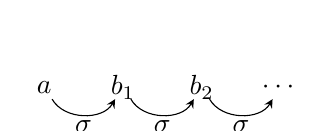
\begin{tikzpicture}
				\node at (0, 0)  {$a$};
				\node at (1, 0)  {$b_1$};
				\node at (2, 0)  {$b_2$};
				\node at (3, 0)  {$\cdots$};
				\draw[-stealth]   (0.1,-0.15) to[out=-60,in=-120](0.9,-0.15);
				\node at (0.5, -0.5)  {$\sigma$};
				\draw[-stealth]   (1.1,-0.15) to[out=-60,in=-120](1.9,-0.15);
				\node at (1.5, -0.5)  {$\sigma$};
				\draw[-stealth]   (2.1,-0.15) to[out=-60,in=-120](2.9,-0.15);
				\node at (2.5, -0.5)  {$\sigma$};
			\end{tikzpicture}
		\end{center}
		Then for all $k\in\mathbb{N}^+$, $aFb_k$ and $\models S_{km}(a,b_k)$ and $\models \neg S_{kn}(a,b_k)$. Since  $\models S_{km}(a,b_k)$ and $b_k$ is not related to anything in $\C$, we get $\bigwedge_{q\in \mathbb{Q}^+ } \bigwedge_{c \in \C} \neg S_q(a, -b_k + c)$, 
		%%%Krzys rev: I added  $a+b_k \in p(\C')$.
		that is $a+b_k \in p(\C')$.
		As we can use arbitrarily large $k$, by compactness (or rather $|\C|^+$-saturation of $\C'$), there exist $b$  such that $(a,b)$ satisfies $(*)$, a contradiction.
		%and hence, by compactness, $\exists b'\in p(\C')$ such that $aFb'$ and $$\models \bigwedge_{q\in \mathbb{Q}^+ } \neg S_q(a,b').$$ 
		%%%Krzys: The statement below should be proved, as it contains a non-obvious trick. So I added a proof. 
		%In a similar manner, we can produce 
		
		We will show now that there is $b'\in p(\C')$ such that %change 4.14 $$(**)\;\;\;\;\;\; aFb' \;\; \textrm{and}\;\; \models \bigwedge_{c\in\C} \bigwedge_{q\in \mathbb{Q}^+ } \neg S_q(a-b',c) \wedge \neg S_q(a+b',c).$$
		$$(**)\;\;\;\;\;\; aFb' \;\; \textrm{with}\;\; a+b',a-b'\in p(\C').$$
		%%%Either b' already satisfies it, or $a-b'$ is related to some infinite $c\in \C$. In the second case we use compactness, given a finite set of elements $A$, $a-b'$ can only be related to elements of the form $c+r$ where $r\in \R+\mu$. In general, $a-b'_k$ can only be related to elements of the form $kc+r$ where $r\in \R+\mu$. It is clear that after finitely many steps we find some element b'_n satisfying any finite set of $A$ formulas in our type.
		Namely, either $b':=b$ already satisfies it, or $a-b$ is related to some infinite $c\in \C$.  In the latter case, $a-b$ is related precisely to the elements from the set $c+\mathbb{R}+\mu$. 
		
		Let $\sigma\in\auto(\C'/\C)$ be such that $\sigma(a)=b$; set $b_k:=\sigma^k(a)$. 
		%%%Krzys rev: "We get" replace by "We have".
		We have
		
		\begin{center}
			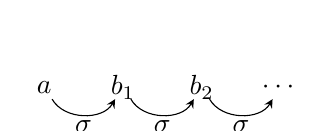
\begin{tikzpicture}
				\node at (0, 0)  {$a$};
				\node at (1, 0)  {$b_1$};
				\node at (2, 0)  {$b_2$};
				\node at (3, 0)  {$\cdots$};
				\draw[-stealth]   (0.1,-0.15) to[out=-60,in=-120](0.9,-0.15);
				\node at (0.5, -0.5)  {$\sigma$};
				\draw[-stealth]   (1.1,-0.15) to[out=-60,in=-120](1.9,-0.15);
				\node at (1.5, -0.5)  {$\sigma$};
				\draw[-stealth]   (2.1,-0.15) to[out=-60,in=-120](2.9,-0.15);
				\node at (2.5, -0.5)  {$\sigma$};
			\end{tikzpicture}
		\end{center}
		%
		Then $aFb_k$, and one easily checks that $a-b_k$ is related precisely to the elements from the set $kc + \R+\mu$, and so $a+b_k$ is not related to anything in $\C$. Since $c$ is infinite, the sets $kc + \mathbb{R} + \mu$ are pairwise disjoint for different $k$'s, and so we find the desired $b'$ using compactness (or rather $|\C|^+$-saturation of $\C'$).
		
		%%%Krzys: I changed the next sentence, as not the terms in $F$ but in the statement of Case 2 matter. I think we do not need to consider $b-ta$. There is no need to use that 1 is in the language. 
		%  Since we are working in a divisible group and $1$ belongs to our language, without loss of generality all the terms in our equivalence relation $F$ are of the from $a-tb$ for $t\in \mathbb{Q}$ (or $b-ta$).
		%%%Krzys final:  ``$t_q(x,y):=x-qy$  for $q\in \mathbb{Q}$ or $t_q(x,y):=qy$ for $q\in \mathbb{Q} \setminus\{0\}$'' in place of ``$t_q(x,y):=x-qy$ or $qy$ for $q\in \mathbb{Q}$ (which is non-zero in the last case)'' .
		%change 4.16 changed the terms as suggested but allowed n to be negative because I think it is necessary to cover all the possible terms, in the suggestion the referee said m,n>0
		Since we are working in a divisible group, %change 4.16a cited our paper
		using Remark \ref{R}, %\cite[Remark 4.6]{10.1215/00294527-2022-0023},
  we can replace the terms $t(x,y)$ in the statement of Case 2 by expressions $t_q(x,y):=nx-my$, where $q=\frac{n}{m}$ is the reduced fraction of $q$
		%%%Krzys rev: I added "(i.e. $\gcd(m,n)=1$ with $m>0$)". It is not true that we can take $m,n>0$ as the referee wrote.
		(i.e. $\gcd(m,n)=1$ with $m>0$). In particular, note that no term of the form $t(x,y)=nx$ or $t(x,y)=my$ can occur in Case 2 hypothesis, since that would contradict $a,b\in p(\C')$.
		%%%Krzys: Slightly modified to reflect the above change of notation. Also, ``for some'' in place of ``for any''.
		%change 4.17 rewrote using the new terms
		Notice that for each %$t_z(x,y):=x-zy$ and 
		$d \in p(\C')$  there exists at most one rational $q$ such that $$S_k(t_q(a,d),c)$$ holds for some $c\in \C$ and $k\in \mathbb{Q}^+$. 
		%%%Krzys rev: I added "(with reduced fractions $\frac{n}{m}$ and $\frac{n'}{m'}$, respectively)".
		For if there existed $q \ne q'\in\mathbb{Q}$ (with reduced fractions $\frac{n}{m}$ and $\frac{n'}{m'}$, respectively), $k,k' \in \mathbb{Q}^+$, and $c,c' \in \C$ such that 
		%%%Krzys rev: I used $q$ and $q'$ instead of the explicit fractions.
		$S_{k}(t_q(a,d),c)$ and $S_{k'}(t_{q'}(a,d),c')$, 
		%%%Krzys rev: $S_{n'k+nk'}((mn'-m'n)d,nc'-n'c)$ instead of $S_{n'k+nk'}((mn'-m'n)d,n'c-nc')$. Check it.
		this would imply $S_{n'k+nk'}((mn'-m'n)d,nc'-n'c)$, contradicting that $d \in p(\C')$ when $mn'-m'n\neq 0$. 
		%%%Krzys: I added the next sentence, as it is silently used below.	
		%change 4.17 This also shows that for every $q \in \mathbb{Q} \setminus \{0\}$, $qd$ is not related to anything in $\C$.
		
		
		%%%Krzys: I expanded the rest, as again, without having in mind a very clear picture of the whole proof, it is difficult to complete this proof.
		%By compactness, there exists $d\in p(\C')$ such that $aFd$ and $$\models \bigwedge_{c\in\C}\neg(R_n(t(a,d),c)\vee R_n(c,t(a,d)))$$ for all terms $t(x,y)$ in the language, contradicting the assumptions of the second case.
		%%%Adrian: Here we are using compactness in the following manner: Either b'' already satisfy what we want or otherwise assume t>1 w.l.o.g (because of the symmetry). In general, a-t^{k+1}b''_k is related to something in \C (we can compute it explicitly). By uniqueness of this parameter $t$, as it keeps growing, we can witness any finite set of formulas from the type if we take b''_k for k big enough. 
		We will show now that there exists $b''\in p(\C')$ such that 
		$$aFb''\;\; \textrm{and} \;\; \models \bigwedge_{q \in \mathbb{Q}} \bigwedge_{n \in \mathbb{Q}^+}\bigwedge_{c\in\C}\neg S_n(t_q(a,d),c),$$ %change 4.17 means we have to erase this too where $t_z(x,y):=x-zy$, 
		contradicting the assumption of Case 2.
		
		Namely, either $d:=b'$ does the job, or there are $q \in \mathbb{Q}$, $n \in \mathbb{Q}^+$, and $c \in \C$ such that  $S_n(t_q(a,b'),c)$. By the choice of $a$ and $b'$ satisfying $(**)$, we have that $q \notin\{-1,0,1\}$.
		
		%%%Krzys rev: "We have"
		Again, let $\sigma\in\auto(\C'/\C)$ be such that $\sigma(a)=b'$; set $b'_k:=\sigma^k(a)$. We have
		
		\begin{center}
			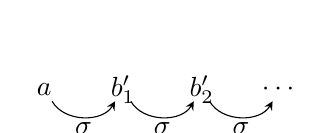
\begin{tikzpicture}
				\node at (0, 0)  {$a$};
				\node at (1, 0)  {$b_1'$};
				\node at (2, 0)  {$b_2'$};
				\node at (3, 0)  {$\cdots$};
				\draw[-stealth]   (0.1,-0.15) to[out=-60,in=-120](0.9,-0.15);
				\node at (0.5, -0.5)  {$\sigma$};
				\draw[-stealth]   (1.1,-0.15) to[out=-60,in=-120](1.9,-0.15);
				\node at (1.5, -0.5)  {$\sigma$};
				\draw[-stealth]   (2.1,-0.15) to[out=-60,in=-120](2.9,-0.15);
				\node at (2.5, -0.5)  {$\sigma$};
			\end{tikzpicture}
		\end{center}
		%
		Then $aFb_k'$ for all $k \in \mathbb{N}^+$. On the other hand, applying powers of $\sigma$, we easily conclude that for every $k \in \mathbb{N}^+$, $t_{q^{k}}(a,b_k')$ is related to some element of $\C$. Hence, by an observation above, we get that for all rationals $r \ne q^k$, $t_r(a,b_k')$ is not related to anything in $\C$. Since $q \notin\{-1,0,1\}$, we know that $q,q^2,\dots$ are pairwise distinct.  So, by compactness, the desired $b''$ exists.
	\end{proof}
	
	%%%Krzys rev: $\C$-small
	\begin{claimnum}
		$F \cap E$ is either equality, or $ E$, or $E_A$ for some non-empty $\C$-small set $A$ of positive infinitesimals in $\C$.
	\end{claimnum}
	
	\begin{proof}[Proof of Claim]
		
		%%%Krzys: The proof below was not clear tome. In particular, why only the Boolean combinations mentioned below are sufficient, and more importantly why the displayed set determines $F$. It is possible that the proof works, but more details should be given. 
		%%%Krzys: I wrote a different proof, in the spirit of the above arguments.
		
		%%%%%%%%%%%%%%%%%%%%%%%%%%%%%%%%%%%%%%%%%%%%%%%%%%%%%%%%%%
		\begin{comment}	
		Finally, we study the relatively-type-definable equivalence relations that are finer than $E\upharpoonright_{p}$ and different from equality. Using quantifier elimination, it is not hard to show that any relatively-type-definable (over a small $A\subseteq \C$) equivalence relation $F$ on $p(\C')$ finer than $E\upharpoonright_{p}$ and different from equality is equivalent to $E\upharpoonright_{p}$ intersected with some partial type consisting of Boolean combinations of formulas of the form $x-y\leq a_1$, $y-x\leq a_2$, where $a_1$ and $a_2$ belong to a small subset of positive infinitesimals $A'\subseteq \C$.
		%%%Adrian: The way to show this is to take any formula $R_n(t(x,y),c)$ and show that under $E\upharpoonright_p$ the only non-trivial formulas are when  t(x,y) is x-y or y-x and c is in n+\mu. The same for the negation. 
		The set $$ \{ a-b: aFB; \hspace{4pt} a,b\in p(\C') \} $$ is a subgroup of the infinitesimals and clearly determines the equivalence relation $F$. 
		Hence, it is enough to study the non trivial type-definable subgroups (over a small set of parameters $A'$ composed of positive infinitesimals) of the infinitesimals $\mu$ in a monster model $\C$ of $(\mathbb{R},+,-,1,\leq)$. Let $S$ be such a group. Without loss of generality, $A'$ is closed under sums, differences and dividing by positive natural numbers. 
		%%%Adrian: we are in a divisible group.
		The set $B=\{a\in A': \forall s\in S(a\geq s)\}$ is closed under the operation of dividing by a natural number. Otherwise, there is $a\in B$, $s\in S$ and $n\in\mathbb{N}^+$ such that $a/n\leq s\leq a$, since $S$ is a group, $(n+1)s\geq a$ which is a contradiction with $a\in B$. There are 2 cases:
		
		Case 1: $B$ is empty. This means that by compactness, we can find $s\in S$ such that for all $a\in A'$ $s>a$. By o-minimality, all elements in $\mu$ satisfying those conditions have the same type over $A'$. By symmetry of $S$, we focus only on the positive part. For any $a\in\mu^+$, the elements $s+a$ and $s$ have the same type over $A'$, hence $S=\mu$. We conclude that $F=E$.
		
		Case 2: $B$ is not empty. We want to show that $S$ is the set $$\{x\in\mu: \forall b\in B(-b<x<b) \}.$$ We will focus in the positive part of $S$. By compactness, there is a positive $s\in S$ bigger than any element in $A'\setminus B$ and smaller than any $b\in B$. By o-minimality, all elements in $\mu$ satisfying those conditions have the same type over $A'$. If $$S\neq \{x\in\mu: \forall b\in B(-b<x<b) \},$$ then there is $a'\in \mu^+$ such that $a'\not\in S$. The elements $s+a'$ and $s$ have the same type, hence both belongs to $S$, but this is a contradiction with $a'\not\in S$. Hence, $F$ is the equivalence relation on $p(\C')$ defined by  $$\bigwedge_{b\in B}\bigwedge_{r\in \mathbb{Q}^+ }(R_r(x-y,b)\vee R_r(y-x,b)).$$	
		\end{comment}
		%%%%%%%%%%%%%%%%%%%%%%%%%%%%%%%%%%%%%%%%%%%%%%%%%%%%%%%%%%%%%
		
		
		
		%%%Krzys rev: $\C$-small
		We may assume that $F \subseteq E $, and just work with $F$. Let $B$ be a $\C$-small $\dcl$-closed subset of $\C$ over which $F$ is relatively defined on $p(\C')$. Extending the notation from before the statement of Theorem \ref{theorem: classification}, for any $B' \subseteq B$ put $$E_{B'}: =\{(x,y) \in p(\C')^2: \bigwedge_{b \in B'^{+}} \bigwedge_{n \in \mathbb{N}^+} |y-x| \leq \frac{1}{n}b\},$$
		where %change 4.19 added b \geq 1
		$B'^{+}:= \{ b \in B': 0< b \leq 1\}$. Let $A := \bigcup\{B' \subseteq B: F \subseteq E_{B'}\}$. Then 
		$$F \subseteq \bigcap \{E_{B'}: B' \subseteq B \;\; \textrm{such that}\;\; F \subseteq E_{B'}\} = E_A,$$
		and, as $F \subseteq E $, we have that $1 \in A$.
		
		We will show that either $F$ is equality, or $F= E_A$. This will clearly complete the proof of the claim (note that if $A$ does not contain any positive infinitesimals, then $E_A = E$).
		%%%Adrian2: changed $E\ne =$ for $E$ is not the equality because it still fits in the line and I think I like it a bit more.
		Suppose $F$ is not the equality. It remains to show that $F \supseteq E_A$.
		
		Case 1: $A=B$. Pick any distinct $\alpha ,\beta \in p(\C')$ such that $\alpha F\beta $. 
		%Since $\alpha \equiv_\C - \alpha$, we can assume that $\alpha>0$. 
		%%%Adrian2: displated the next formula
		Then $$\bigwedge_{a \in A^+} |\alpha-\beta| \leq a.$$ Consider any $\alpha',\beta'  \in p(\C')$ with $\alpha'E_A\beta'$. Then either $\alpha'=\beta'$ (and so $\alpha'F\beta'$), or $\bigwedge_{a \in A^+} 0<|\beta'-\alpha'|\leq a$. In the latter case, it remains to show that $\alpha \beta \equiv_A \alpha' \beta'$  or $\alpha \beta \equiv_A \beta'\alpha'$ 
		%%%Adrian2: changed $F$ is $A$ invariant to $F$ is relatively typee-definable over $A$ (it is over $B$ but in this case B=A)
		(as then $\alpha'F\beta'$, since $F$ is relatively type-definable over $A$). Without loss of generality, $\beta > \alpha$ and $\beta'>\alpha'$; equivalently, $R_1(\alpha,\beta)$ and $R_1(\alpha',\beta')$ both hold. Since $\alpha \equiv_{\C} \alpha'$, we can assume that $\alpha=\alpha'$. It suffices to show that $$\{0<t-\alpha \leq a: a \in A^+\}$$ determines a complete type over $\dcl(A,\alpha)$. 
		%%%Krzys rev: I prefer the shorter version, so I changed it.
		By o-minimality %change 4.21a added property
		of $(\mathbb{R},+,-,1,\leq)$, this boils down to showing that there is no $b \in \dcl^*(A,\alpha)$ with $\bigwedge_{a \in A^+} \alpha<b\leq\alpha+a$, where $\dcl^*$ is computed in the language $\{+,-,1,\leq\}$. If there was such a $b$, then, by q.e. for the theory of divisible ordered abelian groups,  
		%%%Krzys final: I replaced $\beta$ by $\gamma$ below, as $\beta$ was already in the analysis of Case 1.
		it would be of the form $\gamma + q\alpha$ for some $\gamma \in A$ and $q \in \mathbb{Q}$, and we would have $\bigwedge_{a \in A^+} 0< \gamma +(q-1)\alpha \leq a$. If $q=1$, we get %change 4.21 
		$0<\gamma\leq \frac{1}{2}\gamma<\gamma$, a contradiction. If $q \ne 1$, we get that $\alpha$ is related to an element of $A$ which contradicts the fact that $\alpha \in p(\C')$.
		
		Case 2: $A \subsetneq B$. 
		%%%Krzys rev: I changed the next sentence.
		Take any $b\in B\setminus A$. 
		%%%Krzys rev: $F\nsubseteq E_{A\cup \{b\}}$ instead of $F\subsetneq E_{A\cup \{b\}}$. Also, I added "=E_A \cap A_b$; swapping $x$ and $y$ if necessary, we may assume that $y>x$".
		Then, by maximality of $A$, $F\nsubseteq E_{A\cup \{b\}}$, so there is $(x,y)\in F$ such that $(x,y)\notin  E_{A\cup \{b\}}=E_A \cap E_b$; swapping $x$ and $y$ if necessary, we may assume that $y>x$. As $F\subseteq E_A$, we have that $(x,y)\notin E_b$. %change 4.22 comment: he sais that b\in B^+ but that is not true, however, it is true that either b or -b is in B^+. Note that this change is important and affects the notation 
		%%%Krzys rev: I changed the part below to something very close to what the referee wrote.
		%In particular this implies that either $b$ or $-b$ belongs to $B^+$. We can assume that $b\in B^+$ and hence $\lvert y-x \rvert > \frac{1}{n}b$ for some $n\in \mathbb{N}$. 
		%%%Krzys rev: $\mathbb{N}^+$ twice instead of $\mathbb{N}$.
		In particular, this implies that $b \in B^+$ and $y-x > \frac{1}{n}b$ for some $n\in \mathbb{N}^+$. 
		Since $F\subseteq E_A$, we have that $\lvert y-x \rvert< \frac{1}{n}a$ for all $a\in A^+$ and $n\in \mathbb{N}^+$, concluding $\bigwedge_{a \in A^+} b<a$. 
		%change 4.22 Then we can find $b \in B^+$ such that $\bigwedge_{a \in A^+} b<a$. Consider any such $b$. Then, $F(x,y)$ holds for some $x,y \in p(\C')$ such that $y-x > \frac{1}{n}b$ for some $n \in \mathbb{N}^+$.  Indeed, otherwise $F \subseteq E_{A \cup \{b\}} \subsetneq E_A$, which contradicts the minimality of $E_A$ (note that $E_{A \cup \{b\}} \subsetneq E_A$ is witnessed by $(c,c+b)$ for any $c \in p(\C')$, as $A$ is closed under taking fractions).
		
		%%%Krzys rev: Corrected "set" and "We have".
		Let $\sigma \in\auto(\C'/\C)$ be such that $\sigma(x)=y$; set $y_k:=\sigma^{k}(x)$. We have
		
		\begin{center}
			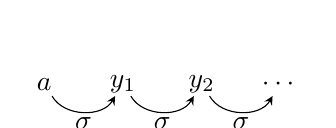
\begin{tikzpicture}
				\node at (0, 0)  {$a$};
				\node at (1, 0)  {$y_1$};
				\node at (2, 0)  {$y_2$};
				\node at (3, 0)  {$\cdots$};
				\draw[-stealth]   (0.1,-0.15) to[out=-60,in=-120](0.9,-0.15);
				\node at (0.5, -0.5)  {$\sigma$};
				\draw[-stealth]   (1.1,-0.15) to[out=-60,in=-120](1.9,-0.15);
				\node at (1.5, -0.5)  {$\sigma$};
				\draw[-stealth]   (2.1,-0.15) to[out=-60,in=-120](2.9,-0.15);
				\node at (2.5, -0.5)  {$\sigma$};
			\end{tikzpicture}
		\end{center}
		%
		We easily conclude that $F(x,y_k)$ and $y_k -x > \frac{k}{n}b$ for all $k$; in particular, $y_n -x>b$. By compactness (or rather $|\C|^{+}$-saturation of $\C'$), there exist $x',y' \in p(\C')$ such that $F(x',y')$ and:
		\begin{enumerate}%change 4.23(b) I decided not to remove 1 even when it is implied by $F$ because I think we want to make enphasis in the fact that only those 2 conditions is enough to guarantee that they have the same type over $B$.
			%%%Krzys rev: I removed the redundant parentheses.
			\item $\bigwedge_{a \in A^+} 0<y'-x'<a$;
			\item $\bigwedge_{b \in B^+\setminus A^+} b<y'-x'$.
		\end{enumerate}
		
		We will check now that whenever $x'',y'' \in p(\C')$ satisfy (1) and (2), then $x'y' \equiv_B x''y''$.
		For that, without loss of generality, we can assume that $x'=x''$. It remains to show that the partial type %change 4.24
		$$\pi(t/x'):= \{0<t-x'<a: a \in A^+\} \cup \{b<t-x': b \in B^+\setminus A^+ \}$$ 
		determines a complete type over $\dcl(B,x')$.  
		%%%Krzys rev: Removed "the" before "o-minimality".
		By o-minimality of $(\mathbb{R},+,-,1,\leq)$, this boils down to showing that there is no $c \in \dcl^*(B,x')$ realizing $\pi(t/x')$, where $\dcl^*$ is computed in the language $\{+,-,1,\leq\}$. If there was such a $c$, then, by q.e. for the theory of divisible ordered abelian groups,  it would be of the form $\beta + qx'$ for some $\beta \in B$ and $q \in \mathbb{Q}$, so %change 4.25
		$$ \bigwedge_{a\in A^+} \bigwedge_{b \in B^+\setminus A^+}  b<\beta +(q-1)x'<a.$$
		%change 4.26
		If $q=1$, we get $\bigwedge_{a \in A^+} 0<\beta<a$, so $\beta \in B^+\setminus A^+$, concluding $\beta < \beta$, a contradiction. 
		%%%Krzys rev: "we get that'' instea of "then".
		If $q \ne 1$, as $1\in A$, we get that $x'$ is related to an element of $B$, which contradicts the fact that $x' \in p(\C')$.
		
		%%%Krzys final: $E_A$ instead of $E_B$; this was an annoying mathematical typo :)
		%change 4.27
		Finally, consider any $(\alpha,\beta) \in E_A$, say with $\beta >\alpha$ so $0<\beta-\alpha<\frac{1}{2}a$ for all $a\in A^+$. 
		%%%Krzys rev: Removed "the", and "b<\alpha-\gamma" instead of (b<\alpha'-\gamma').
		Applying $\sigma \in \auto(\C'/\C)$ mapping $y'$ to $\alpha$, we obtain $\gamma:=\sigma(x')$ such that $\gamma F\alpha$ and $\bigwedge_{b \in B^+\setminus A^+} b<\alpha-\gamma$. Since $F\subseteq E_A$, we get  $b<\alpha -\gamma < \frac{1}{2}a$ for all $b\in B^+\setminus A^+$ and $a\in A^+$. Therefore, $b<\beta - \gamma < a$ for all $b\in B^+\setminus A^+$ and $a\in A^+$, %$(\gamma,\beta)$ also satisfies (1) and (2). Therefore, $\gamma\alpha \equiv_B x'y' \equiv_B \gamma\beta$. As $x'Fy'$, we conclude that $\alpha F \beta$, 
		%%%Krzys I gave some details below.
		%which completes the proof of the claim.
		So, by the previous paragraph, $\gamma \alpha \equiv_B x'y' \equiv_B \gamma\beta$. As $(x',y') \in F$, we conclude that $(\alpha,\beta) \in F$, which completes the proof of the claim.
	\end{proof}
	
	%change 4.28
	%%%Krzys rev: The argument suggested by the referee contains a serious mistake. Namely, "By saturation, there is $c\in \C$ such that $a+b\in c+\mu_A$." is not a correct reasoning. Since $\mu_A$ is of unbounded index in $\mu$, a compactness argument does not work here. Actually to the deduce the theorem from the claims is a more delicate issue that we missed before. Below is a proof.
	%By the above two claims, to conclude the proof of the theorem it suffices to show that if $E_A=E\cap F\subsetneq F \subseteq E_{c_0}^\mu$ for some $c_0$, then $F=E_{A,c}$ for some $c$. Take $(a,b)\in F\setminus E$. Then, $aE_{c_0}^\mu b$, so $a+b\in c_0+\mu$. By saturation, there is $c\in \C$ such that $a+b\in c+\mu_A$. For any $b'\in p(\C')$ with $a+b'\in c+\mu_A$, we get $bE_Ab'$, so $bFb'$, concluding $aFb'$. Therefore $E_{A,c}\subseteq F$. On the other hand, for any other $(a,b')\in F\setminus E$, $a+b\in c_0+\mu$ and $a+b'\in c'+\mu_A$ for some $c'\in \C$. Hence, $bFb'$ and $b-b'\in \mu$, so $b-b'\in\mu_A$ as $E\cap F\in E_A$. Thus, $c_0-c'\in b-b'+\mu_A=\mu_A$, concluding $(a,b')\in E_{A,c}$, so $F\subseteq E_{A,c}$.
	By the above two claims, in order to prove the theorem, it remains to consider the case when $E\cap F\subsetneq F \subseteq E_{c_0}^\mu$ for some $c_0 \in \C$.
	%By the first claim, we have $F \subseteq E_{c_0}^\mu$ for some $c_0 \in \C$.
	By the second claim, we have the following two cases.
	
	Case 1: $E \cap F$ is the equality. We will show that then $F =E_c$ for some $c \in \C$. Consider any $a \in p(\C')$. Since $F \ne \;=$, there exists $b \ne a$ such that $aFb$. Since $F \subseteq E_{c_0}^\mu$ and $E \cap F$ is the equality, we get that such a $b$ is unique: if $b' \ne a$ also satisfies $aFb'$, then $b,b' \in -a+c_0 + \mu$, so $b-b' \in \mu$, hence $b=b'$ because $bFb'$. 
	%This unique $b$ belongs to $\dcl(\C, a)$, so $c:=a+b \in \dcl(\C, a)$. As $T$ has q.e., $c=c' +qa$ for some $c' \in \C$ and $q \in \mathbb{Q}$. The $F$-class of $a$ is the set $\{a,-a+c\}$. Take $\sigma \in \auto(\C'/\C)$ with $\sigma(a)=-a+c$. Then $a=\sigma(-a +c)= a-c +\sigma(c)$, so $\sigma(c)=c$. Hence, $c'+qa= c'+q\sigma(a)=c'-qa +qc =c'-qa+qc'+q^2a$, and so $q(2-q)a =qc' \in \C$. So either $q=0$, and then $c=c' \in \C$, or $q=2$ and $c'=0$, but then $b=-a+c=a$, a contradiction. Applying automorphisms over $\C$, we get $F=E_c$.
	%%%Adrianrev2: added $\dcl$ coincides with the definable closure $\dcl^*$ computed in the language $\{+,-,1,\leq\}$ and its explanation
	This unique $b$ belongs to $\dcl(\C, a)$, so $g:=a+b-c_0 \in \dcl(\C,a) \cap \mu$.
	%%%Krzysrev2: I changed the next two sentences, as we do not need to talk about dcl^* here.
	Since $a$ is not related to any element of $\C$ and $\dcl$ is given by ``terms" with rational coefficients (which follows from q.e. for $T$),  we get that $g \in \C$.
	%Since $T$ has q.e., $a$ is not related to any element of $\C$ and $\dcl$ coincides with the definable closure $\dcl^*$ computed in the language $\{+,-,1,\leq\}$ (this follows from the fact that $\dcl^*$ is given by ``terms" with rational coefficients), we get that $g \in \C$. 
	Hence, $c:=a+b=c_0+g \in \C$. Applying automorphisms over $\C$, we get $F=E_c$.
	
	Case 2: $E \cap F=E$ or $E \cap F=E_A$ for some non-empty $\C$-small set $A$ of positive infinitesimals. Since $E=E_{\{1\}}$ (with the obvious extension of the definition of $E_A$), we can write $E \cap F=E_A$, where $A$ is either a non-empty $\C$-small set $A$ of positive infinitesimals or $A=\{1\}$. We will show that then $F =E_{A,c}$ for some $c \in \C$, where $E_{\{1\},c}:=E^\mu_c$. Extend the definition of $\mu_A$ via $\mu_{\{1\}}:=\mu$.
	
	%%%Adrianrev2: It used to say ' Since $E\cap F \ne E$' instead, I think it was a typo
	Consider any $a \in p(\C')$. Since $E\cap F \ne F$ and $F \subseteq E_{c_0}^\mu$, there exists $b\in p(\C')$ such that $(a,b) \in F \setminus E$ and $a+b = c_0 +g$ for some $g \in \mu$. As  $E \cap F=E_A$, we get that $\sigma(g)-g \in \mu_A$ for every $\sigma \in \auto(\C'/\C a)$. 
	
	%We claim that $g \in \dcl(\C, a) + \mu_A$. For that first note that $\dcl$ coincides with the definable closure $\dcl^*$ computed in the language $\{+,-,1,\leq\}$ (this follows from the fact that $\dcl^*$ is given by ``terms" with rational coefficients). Hence, if  $g \notin \dcl(\C, a) + \mu_A$, then $(g+\mu_A) \cap \dcl^*(\C, a) = \emptyset$, and so, by o-minimality of $(\mathbb{R},+,-,1,\leq)$, the orbit of $g$ under $\auto(\C'/\C a)$ is not contained in $g + \mu_A$, a contradiction.
	%We claim that $g \in \dcl(\C, a) + \mu_A$. 
	%Adrianrev2 moved this sentence %For that first note that $\dcl$ coincides with the definable closure $\dcl^*$ computed in the language $\{+,-,1,\leq\}$ (this follows from the fact that $\dcl^*$ is given by ``terms" with rational coefficients). 
	%%%Adrianrev2:modified the paragraph according to the suggestion of the referee
	%%%Krzysrev2: In the new version of the paragraph below, I think we have to use weak inequalities around $g$, so I did it.
	Since $\sigma(g)-g \in \mu_A$ for every $\sigma \in \auto(\C'/\C a)$, we conclude by o-minimality of $(\mathbb{R},+,-,1,\leq)$ that, for every $\alpha\in A$ and $\in \mathbb{N}^+$, there are $c_{\alpha,n}, d_{\alpha,n} \in \dcl^*(\C,a)$ such that $g-\frac{1}{n}\alpha<c_{\alpha,n}\leq g\leq d_{\alpha,n}<g+ \frac{1}{n}\alpha$, 
	%%%Krzysrev2: I added the rest of this sentence "where...".
	where  $\dcl^*$ is the definable closure computed in the language $\{+,-,1,\leq\}$ (which coincides with $\dcl$ as both closures are given by ``terms" with rational coefficients). 
	%%%Krzysrev2: I removed "using q.e. and" as it is redundant. Also "is given by" in place of "consists of". Also $\dcl^*$ in place of $\dcl$ (although they are the same).
	Since $a$ is not related to any element of $\C$ and for every $\alpha\in A$ and $n\in \mathbb{N}^+$ the elements $c_{\alpha,n}, d_{\alpha,n}$ are related to zero, using that $\dcl^*$ is given by  ``terms'' with rationals coefficients, we conclude that $c_{\alpha,n}$ and $d_{\alpha,n}$ belong to $\C$ for every $\alpha\in A$ and $n\in \mathbb{N}^+$. Since $A$ is $\C$-small, the set of all $c_{\alpha,n}$ and $d_{\alpha,n}$ is $\C$-small, and hence there is $e \in \C$ with $g-\frac{1}{n}\alpha< e <g + \frac{1}{n}\alpha$ for all $\alpha \in A$ and $n \in \mathbb{N}^+$. Then, $g\in e+\mu_A$ with $e\in \C$, concluding $a+b\in c+\mu_A$, where $c=c_0+e\in \C$, so $aE_{A,c}b$.
	%Then $e \in \dcl^*(\C,a) \cap (g + \mu_A)$, a contradiction.
	%By q.e. and the fact that $a$ is not related to any element of $\C$, there exists $q \in \mathbb{Q}$ such that for all $\alpha \in A$ and $n \in \mathbb{N}^+$ we have $c_{\alpha,n} = c_{\alpha,n}'+ qa$ and $d_{\alpha,n}=d_{\alpha,n}' +qa$ for some $c_{\alpha,n}',d_{\alpha,n}' \in \C$. Then $g-qa-\frac{1}{n}\alpha<c_{\alpha,n}'<g-qa<d_{\alpha,n}'<g -qa + \frac{1}{n}\alpha$. Since $A$ is $\C$-small, the set of all $c_{\alpha,n}'$ and $d_{\alpha,n}'$ is $\C$-small, and hence there is $e \in \C$ with $g-qa-\frac{1}{n}\alpha< e <g -qa + \frac{1}{n}\alpha$ for all $\alpha \in A$ and $n \in \mathbb{N}^+$. Then $e+qa \in \dcl^*(\C,a) \cap (g + \mu_A)$, a contradiction.
	%Since $g \in \dcl(\C, a) + \mu_A$, using q.e. and the fact that  $g \in \mu$ and $a$ is not related to any element of $\C$, we get that $g \in \C + \mu_A$, so 
	%$c_0+g=c+d$ and $b=-a + c+ d$, where $d \in \mu_A$ and $c\in \C$. 
	\begin{comment}	
	Take $\sigma \in \auto(\C'/\C)$ with $\sigma(a)=-a+c+d$. Then $\sigma(-a+c+d) = a +\sigma(c)-c + \sigma(d)-d=a+\sigma(d)-d$
	%Thus, $c_0+g=c+d$ and $b=-a + c+ d$, where $d \in \mu_A$ and $c=c'+qa$ for some $c' \in \C$ and $q \in \mathbb{Q}$. Take $\sigma \in \auto(\C'/\C)$ with $\sigma(a)=-a+c+d$. Then $\sigma(-a+c+d) = a +\sigma(c)-c + \sigma(d)-d$
	%\in a +\sigma(c)-c + \mu_A$ 
	is $F$-related to $a$. %Since $F \subseteq E_{c_0}^\mu$ and  $E \cap F=E_A$,  we get two subcases.
	%and $a +\sigma(c)-c + \sigma(d)-d+a$ is not comparable with $c_0$, hence $\sigma(c)-c \in \mu_A$
	\end{comment}
	%This yields $(a,b) \in E_{A,c}$.
	
	From the conclusion of the previous paragraph and the fact that $E \cap F=E_A$, we obtain $(a+\mu_A) \cup (-a+ c +\mu_A) \subseteq [a]_F$. By automorphisms over $\C$, the same is true for any other element of $p(\C')$ in place of $a$, so $E_{A,c} \subseteq F$. The opposite inclusion easily follows using the assumptions $F \subseteq E_{c_0}^\mu$ and $E \cap F=E_A$. Namely, using automorphisms over $\C$, it is enough to show that $[a]_F \subseteq [a]_{E_{A,c}}$. Consider any $b' \in [a]_F$. Since $(a,b) \in F \setminus E$ and  $F \subseteq E_{c_0}^\mu$, we have that $b' \in a + \mu$ or $b' \in b + \mu$. As $E \cap F=E_A$, we conclude that $b' \in a + \mu_A$ (and so $b'E_{A,c}a$) or $b' \in b+ \mu_A$ (and so $b'E_{A,c}b$ which together with $aE_{A,c}b$ implies $b'E_{A,c}a$).
	\begin{comment}
	contenidos...
	
	Subcase 2a: $(a +\sigma(c)-c + \sigma(d)-d) -a \in \mu_A$. Then $\sigma(c)-c \in \mu_A$. On the other hand, $\sigma(c)-c= c'+q\sigma(a) -c'-qa=c'-qa+qc+qd-c'-qa= q^2a-2qa+qc'+qd$. If $q \ne 0$, then $(q-2)a\in -c' +\mu_A$, so $q=2$ and $c' \in \mu_A$, which implies $c \in 2a+\mu_A$, so $b=-a+c+d \in a + \mu_A$, that is $(a,b) \in E$, a contradiction. Thus, $q=0$, and so $c \in \C$. This yields $(a,b) \in E_{A,c}$. Since $E \cap F=E_A$, we obtain $(a+\mu_A) \cup (-a+ c +\mu_A) \subseteq [a]_F$. By automorphisms over $\C$, the same is true for any other element of $p(\C')$ in place of $a$, so $E_{A,c} \subseteq F$. The opposite inclusion easily follows using the assumptions $F \subseteq E_{c_0}^\mu$ and $E \cap F=E_A$. Namely, using automorphisms over $\C$, it is enough to show that $[a]_F \subseteq [a]_{E_{A,c}}$. Consider any $b' \in [a]_F$. Since $(a,b) \in F \setminus E$ and  $F \subseteq E_{c_0}^\mu$, we have that $b' \in a + \mu$ or $b' \in b + \mu$. As $E \cap F=E_A$, we conclude that $b' \in a + \mu_A$ (and so $b'E_{A,c}a$) or $b' \in b+ \mu_A$ (and so $b'E_{A,c}b$ which together with $aE_{A,c}b$ implies $b'E_{A,c}a$).
	
	Subcase 2b:  $(a +\sigma(c)-c + \sigma(d)-d) +a \in c_0 + \mu$. Then $2a+\sigma(c)-c -c_0 \in \mu$. On the other hand, $2a+\sigma(c)-c -c_0 = 2a+c'+q\sigma(a)-2c'-2qa-d+g=(q-1)(q-2)a +qc'-c' +qd-d+g$. So $(q-1)(q-2)a +qc'-c' \in \mu$. Therefore, $q=1$ or $q=2$. If $q=1$, then $c=c'+a$, so $b=c'+d \in c' +\mu_A$ which is impossible as $b \in p(\C')$.
	%Hence, applying automorphisms over $\C$, we keep $b+\mu$, while we get infinitely many copies of $a+\mu$. This contradicts the assumption that $F \subseteq E_{c_0}^\mu$. 
	If $q=2$, then $c' \in \mu$ and $c=c'+2a$, so $b=a+c'+d \in a +\mu$, so $(a,b) \in E$, a contradiction.
	\end{comment}
\end{proof}

%%%Krzys rev: $\C$-small
\begin{cor}
	The equivalence relation $E$ is the finest equivalence relation on $p(\C')$ relatively type-definable over a $\C$-small set of parameters of $\C$ and with stable quotient, that is $E^{\textrm{st}}=E$
\end{cor}
\begin{proof}
	The quotient $p(\C')/E$ is stable by Proposition \ref{proposition: stable quotient}. %\cite[Proposition 4.9]{10.1215/00294527-2022-0023}. 
	%%%Krzys rev: I removed parentheses, and wrote $\C$-small.
	Let $F$ be a relatively type-definable over a $\C$-small subset of $\C$ equivalence relation on $p(\C')$ strictly finer than $E$. 
	%%%Krzys final: I added the next sentence.
	%%%Krzys rev: $\C$-small
	By Theorem \ref{theorem: classification}, $F=E_A$ for some non-empty $\C$-small set $A$ of positive infinitesimals in $\C$. 
	%%%Krzys rev: I added "(There is also the case when $F$ is the equality, but then $p(\C')/F=p(\C')$ is clearly unstable.)".
	(There is also the case when $F$ is the equality, but then $p(\C')/F=p(\C')$ is clearly unstable.)
	%%%Krzys: Slightly changed	
	%	By the previous theorem, there is some infinitesimal $c\in \C'$ bigger than all infinitesimals in $\C$ such that for any $a\in p(\C')$ the elements $a$ and $a+c$ are not $F$-related.
	%%%Krzys final: I did not see now how the formula $R_1(x,y)$ works at the end of the proof just using that $a$ and $a+c$ are not $F$-related. So I changed the end of this paragraph.
	%Take any infinitesimal $c\in \C'$ bigger than all infinitesimals in $\C$. By the previous theorem, for any $a\in p(\C')$ the elements $a$ and $a+c$ are not $F$-related.
	%%%Krzys rev: I added ``and'' before ``such that'' to make it more clear. But now it seems to me that the next sentence was to weak to apply it in the next paragraph, as this sentence was a V-definable condition, so there is no reason to be preserved under finding an  indiscernible sequence  by Ramsey's theorem and compactness. So I changed it.
	% One easily concludes that for every $a,d,e\in p(\C')$ and infinitesimal $c\in \C'$ bigger than all infinitesimals in $\C$ and such that $d F a$ and $e F (a+c)$, we have $d<e$, and so $\neg R_1(e,d)$.
	
	Pick any $\alpha \in A$.
	It is easy to check that for every $a,d,e\in \C'$ and infinitesimal $c\in \C'$ bigger than all infinitesimals in $\C$ and such that $|d - a|\leq \frac{1}{2}\alpha$ and $|e -(a+c)|\leq\frac{1}{2}\alpha$, we have $d<e$, and so $\neg R_1(e,d)$. And note that ``$|x-y|\leq\frac{1}{2}\alpha$'' can be written as an $L_\alpha$-formula.
	
	
	%%%Adrian: Very similar to the previous example
	%%%Adrian:(Alternative proof) Take a sequence $(c_i)_{i<omega}$ of infinitesimal of $\C'$ bigger than all infinitesimals in $\C$ such that $c_i$ is infinitesimal with respect to $c_{i+1}$. The sequence $(a+c_i)_{i<$\omega$}$ is $\C$-indiscernible  but not totally-$\C$-indiscernible since the formula $R_1(x,y)$ witnesses that $$ \tp([a+c_i]_F,[a+ c_{i+1}]_F/ \C)\neq\tp([a+c_{i+1}]_F, [a+c_i]_F/ \C). $$
	%%%Adrian: To see that the sequence is $\C$-indiscernible, note that given a subtuple tuple, any operation you do with its component either belongs to p(\C') or it is some infinitesimal (it can be 0 only in trivial cases) and this only depends on which operation we are choosing. The more delicate case is the one where it is some infinitesimal, because it could be a positiver or a negative infinitesimal (bigger/smaller than all infinitesimals in $\C$ respectively). In that case, it only depends on the sign that the operation assigns to the highest index (+ka_{i_n} or -ka_{i_n})
	
	%%%Krzys final: I added the next sentence.
	Take any $a \in p(\C')$ and infinitesimal $c\in \C'$ bigger than all infinitesimals in $\C$.
	%%%Krzys rev: Instead of ``we extract a $\C$-indiscernible sequence $(a_i')_{i<\omega}$ from the sequence $(a+kc)_{k<\omega}$'' I wrote `` we find a $\C$-indiscernible sequence $(a_i')_{i<\omega}$ having the same Erenfeucht-Mostowski type as the sequence $(a+kc)_{k<\omega}$.'' This is important, as extracting is reserved for something slightly different that makes a difference here (since here it is not extracting, there was a problem with the application of the previous paragraph in the last version of the paper; it could be fixed choosing a suitable very long sequence here and then extracting, but I decided to change the previous paragraph instead))
	Using Ramsey's theorem and compactness, 
	%we extract a $\C$-indiscernible sequence $(a_i')_{i<\omega}$ from the sequence $(a+kc)_{k<\omega}$. 
	we find a $\C$-indiscernible sequence $(a_i')_{i<\omega}$ having the same Erenfeucht-Mostowski type as the sequence $(a+kc)_{k<\omega}$.
	Then, the sequence $([a'_i]_F)_{i<\omega}$ is $\C$-indiscernible but not totally $\C$-indiscernible, since the formula $R_1(x,y)$ witnesses that $$ \tp([a'_i]_F,[a'_{i+1}]_F/ \C)\neq\tp([a'_{i+1}]_F, [a'_i]_F/ \C). $$ 
	%%%Krzys: Changed the last sentence.
	%	 Which is a contradiction with indiscernibility by \cite[Theorem 2.10]{10.1215/00294527-2022-0023}
	Thus, $p(\C')/F$ is unstable.%change 4.29c by virtue of \cite[Theorem 2.10]{10.1215/00294527-2022-0023}.
	%%%Adrian: The original sequence does not work directly because (a,a+2c,a+8c,a+9c) does not have the same type as (a,a+2c,a+7c,a+9c). Even over the emptyset.
\end{proof}




\begin{comment}


\section{Discussing the cardinal in the theorem}

We set some notation first $\beth_0(\lambda)=\lambda$, $\beth_{\alpha+1}(\lambda)=2^{\beth_{\alpha}(\lambda)}$ and for limits we take unions. If we omit $\lambda$, it means $\lambda=\omega$.

Let us go through all the requirements for $\nu$ in the proofs of Theorem \ref{Est exists} and Lemma \ref{existence of an special index}. In the proof of the claim, we need that $\nu$ is long enough to extract a subsequence such that all partial types $\pi_{i,\alpha}(x,y,z)$ are equal and all $B_{\alpha,i_\alpha}$ have the same type over $A$. The first requirement is being bigger than $2^{\lvert x \rvert+\lvert y \rvert+\lvert z \rvert+\lvert T\rvert}$, where the size of $x$ and $y$ is something small (we are using only a countable subset of the full tuple $x$ used on $p(x)$) and the size of $z$ can be bounded by $2^{(\lvert T\rvert+\lvert A\rvert)}$ (since we are using a countable amount of variables). The second requirement is being bigger than $2^{2^{\lvert T \rvert+\lvert A \rvert}}$ (because we are counting types over $A$ with $2^(\lvert T \rvert+\lvert A\rvert)$ variables.). Then we call Lemma \ref{existence of an special index}, for that we need $\nu>\beth_{(2^{2^{(\lvert T\rvert + \lvert A\rvert)}})^+}$ or $\beth_{(\beth_{2}(\lvert T \rvert + \lvert A\rvert))^+}$. Of course, $\nu$ has to be small.

In the main proof of the theorem, we first call extracting indiscernibles to claim that w.l.o.g the sequence is $A$ indiscernible. The requirement for this is already satisfied, then, we call again Lemma \ref{existence of an special index}, we don't need to increase $\nu$ for this because it is already big enough.

Hence, we need 
\begin{align*}
\nu>&2^{\lvert x \rvert+\lvert y \rvert+\lvert z \rvert+\lvert T\rvert}\\
\nu>&2^{(\lvert T\rvert+\lvert A\rvert)}\\
\nu>&\beth_{(\beth_{2}(\lvert T \rvert + \lvert A\rvert))^+}
\end{align*}

$\nu>\beth_{(\beth_{2}(\lvert x \rvert+\lvert T \rvert + \lvert A\rvert))^+}$ is enough, and it is the shortest condition that I can think that implies the three above.
\end{comment}
\section{Generalized indiscernibles}\label{section: modelling property}
Let $\mL'$ be a first-order language and $\mL$ be a continuous logic language. Unless specified otherwise, $T$ is a complete continuous $\mL$-theory with $\C\models T$ a monster model (i.e. $\kappa$-saturated and strongly $\kappa$-homogeneous for a strong limit cardinal $> |T|$) and $\I,\mathcal{J}$ are $\mL'$-structures. %All the tuples considered are of length strictly less than $\kappa$, similarly, all the sets considered are small (i.e. of size strictly less than $\kappa$).
As in Chapter \ref{Chapter 3}, we will use the formalism from \cite[Subsection 3.1]{hrushovski2021amenability} and \cite[Section 3]{hrushovski2021order} and adapt some results from \cite{MR2657678}.  In particular, by a {\em CL-formula over $A$} we mean a continuous function $\varphi \colon S_n(A)\to \mathbb{R}$.  If $\varphi$ is such a CL-formula, then for any $\bar b\in M^n$ (where $M \models T$) by $\varphi(\bar b)$ we mean $\varphi(\tp(\bar b/A))$.%; note that the range of every CL-formula is compact. So a CL-formula can be thought of as a function from $\C^n$ to $\mathbb{R}$ which factors through $S_n(A)$ via a continuous map $S_n(A) \to \mathbb{R}$.
%What are called {\em definable predicates}, in finitely many variables and without parameters,  in \cite{MR2657678} are precisely CL-formulas over $\emptyset$, but where the range is contained in $[0,1]$. In any case, a CL-formula can be added as a new CL-predicate and then it becomes a legitimate formula in the sense of continuous logic. 
In the sections concerning hyperdefinable sets, we allow the domain of a CL-formula to be an infinite Cartesian power of $\C$ (which is necessary to deal with $X/E$ in the case when $X\subseteq \C^\lambda$ where $\lambda$ is infinite).%, but still the results from \cite{MR2657678} 
%and \cite{MR2723787} 
%which we will be using are valid for such generalized continuous logic formulas.

In this section, we present natural adaptations of the concepts of generalized indiscernibles and the modeling property to continuous logic and give a characterization of the continuous modeling property in the form of a continuous logic counterpart of \cite[Theorem 2.10]{SCOW2021102891}.

The following idea first appeared in \cite[Definition VIII.2.4]{Shelah1982-SHECTA-5}.

\begin{defin}\label{defin: gen. indisc.}%[Generalized indisc]
    %Let $\mathcal{L}'$ be a first order language and $\mathcal{I}$ an $\mathcal{L}'$-structure. 
    Let $\II=(a_i: i\in \I)$ be an $\I$-indexed sequence, and let $A\subset \C$ be a small set of parameters.  We say that $\II$ is an $\I$-\emph{indexed indiscernible sequence over} $A$ if for all $n\in\omega$ and all sequences $i_1,\dots,i_n,j_1,\dots,j_n$ from $\I$ we have that 
    $$\qftp(i_1,\dots,i_n)=\qftp(j_1,\dots,j_n) \implies \tp({a}_{i_1}, \dots, {a}_{i_n}/A)=\tp({a}_{j_1}, \dots, {a}_{j_n}/A).$$
\end{defin}

We will refer to $\I$-indexed indiscernible sequences as $\I$-indiscernibles.

Next, we adapt the definition of \emph{locally based on} given in \cite{10.1215/00294527-3132797}. The first reference to this concept can be found in \cite{MZiegler}.
 

\begin{defin}[Locally based on] 
%Let $\I$ and $\mathcal{J}$ be $\mL'$-structures and 
Let $\II=(a_i:i\in \I)$ be an $\I$-indexed sequence. We say that a $\mathcal{J}$-indexed sequence $(b_j:j\in\mathcal{J})$ is \emph{locally based on $\II$} if for any finite set of $\mL$ formulas $\Delta$, any finite tuple $\overline{j}\subseteq \mathcal{J}$ and $\varepsilon>0$ there is $\overline{i}\subseteq \I$ such that:
\begin{enumerate}
    \item $\qftp(\overline{i})=\qftp(\overline{j})$ in the language $\mL'$.
    \item $\lvert \varphi(b_{\overline{j}})- \varphi(a_{\overline{i}}) \rvert\leq \varepsilon$ for all $\varphi\in \Delta$.
\end{enumerate}
\end{defin}

 The original definition presented in \cite[Definition 2.5]{10.1215/00294527-3132797} is the following:
 \begin{defin}[Classical definition of Locally based on]
%Let $\I$ and $\mathcal{J}$ be $\mL'$-structures and 
Let $\II=(a_i:i\in \I)$ be an $\I$-indexed sequence. We say that a $\mathcal{J}$-indexed sequence $(b_j:j\in\mathcal{J})$ is \emph{locally based on $\II$} if for any finite set of $\mL$ formulas $\Delta$ and any finite tuple $\overline{j}\subseteq \mathcal{J}$ there is $\overline{i}\subseteq \I$ such that:
\begin{enumerate}
    \item $\qftp(\overline{i})=\qftp(\overline{j})$.
    \item $\tp^{\Delta}(b_{\overline{j}})= \tp^{\Delta}(a_{\overline{i}})$.
\end{enumerate}
\end{defin}
 
 Note that if we tried to use this stronger version of the property, it is easy to show that even for $\I=(\mathbb{N},<)$ we can find a sequence for which there are no indiscernible sequences locally based on it. Consider for example the theory $\Th([0,1],d)$ where $d$ is the distance predicate and the sequence $(1/n)_{n<\omega}$.

The next definition is then the natural continuous counterpart of \cite[Definition 2.17]{SCOW20121624}.

\begin{defin}[Continuous Modeling property]\label{definition: CMP}
    %Fix an $\mL'$ structure $\I$. 
    Given a continuous theory $T$, we say that \emph{$\I$-indexed indiscernibles have the continuous modeling property in $T$} if given any $\I$-indexed sequence $\II=(a_i:i\in \I)$ in a monster model $\C$ of $T$ there exists an $\I$-indiscernible sequence $(b_i:i\in\I)$ in $\C$ locally based on $\II$. We say that $\I$ has the \emph{continuous modeling property} if $\I$-indexed indiscernibles have the continuous modeling property in every continuous theory.
\end{defin}

If a first-order structure $\I$ has the continuous modeling property then it has the modeling property. First, note that given a classical first-order theory $T$, there always exists a continuous logic theory $T'$ such that any model of $T'$  is a model of $T$ with the discrete metric. We show that the following holds:

\begin{prop} \label{CMP implies MP}
    Let $T$ be a first-order theory and let $T'$ be its continuous logic counterpart. Then $\I$ has the continuous modeling property in $T'$ if and only if $\I$ has the modeling property in $T$.
\end{prop}

\begin{proof}
    Clearly, If $\I$ has the continuous modeling property in $T'$ then it has the modeling property in $T$ since classical formulas are a subset of the $\{0,1\}$-valued continuous logic formulas.

    Assume now that $\I$ has the modeling property in $T$. Let $\II=(a_i:i\in \I)$ be any sequence in $\C\models T$. Since $\I$ has the modeling property, there is an $\I$-indiscernible sequence $(b_i:i\in \I)$ locally based on $\II$ (in the classical sense). We show that the sequence $(b_i:i\in \I)$ is locally based on $\II$ in our continuous logic sense. Note that first-order formulas generate a subalgebra $$\mathcal{A}=\bigcup_{n<\omega} \{ u(\varphi_1,\dots, \varphi_n):  \varphi_1,\dots, \varphi_n \text{ f.o. formulas}; u \text{ CL connective}\}$$ which is a dense subalgebra of the set of all continuous logic formulas. Hence, for each continuous logic formula $f(x)$ and $\varepsilon>0$ there is $\varphi(x)\in \mathcal{A}$ such that $\lvert f(x)-\varphi(x)\rvert \leq \varepsilon/2$. Thus, for any tuples 
    %%%Adrian: we have the following for arbitrary tuples i and j of the same lenght
    $\overline{i},\overline{j}\subseteq \I$ %such that $\qftp(\overline{i})=\qftp(\overline{j})$ 
    and tuples $a_{\overline{j}}, b_{\overline{i} }$ we have $$ \lvert f(a_{\overline{j}}) -f(b_{\overline{i}})\rvert \leq \lvert f(x)-\varphi(x)\rvert + \lvert \varphi(a_{\overline{j}}) -\varphi(b_{\overline{i}}) \rvert + \lvert f(x)-\varphi(x)\rvert \leq \lvert \varphi(a_{\overline{j}}) -\varphi(b_{\overline{i}}) \rvert +\varepsilon.$$
    Finally, note that by the definition of being locally based on (in the classical sense) for any $b_{\overline{i}}$ and finite $\Sigma \subset \mathcal{A}$, there is $\overline{j}$ with the same quantifier free type as $\overline{i}$ such that $ \varphi(b_{\overline{i}})=\varphi(a_{\overline{j}}) $ for every $\varphi\in \Sigma$. 
    %%%Adrian: for $\Delta$ a finite set of continuous formulas we take $\Sigma$ the set of first order formulas used to generate any of the $f \in \Delta$.
    Therefore, the sequence $(b_i:i\in \I)$ is locally based on $\II$ in the continuous sense.
\end{proof}

Next, we define two partial types that will be useful during this section. The first one is a generalization of the classical Ehrenfeucht-Mostowski type (EM-type for short). The second is a type whose realizations are exactly the $\I$-indiscernible sequences. They are based on \cite[Definitions 2.6 and 2.10]{SCOW20121624} respectively.

\begin{defin}%[Generalized EM] 
%$Let $\I$ be an  $\mL'$ structure and  l
Let $\II=(a_i:i\in \I)$ be an $\I$-indexed sequence. The \emph{$EM$-type of $\II$} is the set of all conditions $\varphi(x_{i_1}\dots,x_{i_n})=0$ such that $\varphi(a_{j_1}\dots,a_{j_n})=0$ holds for every $j_1,\dots,j_n\in \I$ with the same quantifier free type as $i_1,\dots,i_n$. That is \begin{align*}
    \emtp(\II)(x_i: i\in \I)=\{& \varphi(x_{i_1},\dots,x_{i_n})=0 :  \varphi \in \mL, i_1,\dots,i_n\in \I  \\ &\text{ and for any } j_1,\dots,j_n\in \I  \text{ such that } \\ &\qftp(j_1,\dots,j_n)=\qftp(i_1,\dots,i_n),   \models\varphi(a_{j_1}\dots,a_{j_n})=0 \}.
\end{align*}
\end{defin}

\begin{defin}%[Ind(I,L)]
    %Let $\I$ be an $\mL'$-structure and $\mL$ a continuous language.
    We define $\Ind(\I,\mL)$ as the following partial type:
    \begin{align*}
       \Ind(\I,\mL)(x_i:i\in \I):= \{& \varphi(x_{i_1},\dots,x_{i_n})= \varphi(x_{j_1},\dots,x_{j_n}):&\\
        & n<\omega, \overline{i}, \overline{j}\subseteq \I, \qftp(\overline{i})=\qftp(\overline{j}), \varphi(x_{i_1},\dots,x_{i_n})\in \mL\}.
    \end{align*}
\end{defin}

Finally, we define what it means for a partial type to be finitely satisfiable in a sequence. 

\begin{defin}[Finitely satisfiable] Let $\Gamma(x_i:i\in \I)$ be an $\mL$-type, and let $\II=(a_i:i\in \I)$ be an $\I$-indexed sequence. We say that $\Gamma$ is \emph{finitely satisfiable in $\II$} if for every finite $\Gamma_0\subseteq \Gamma^+$ and for every finite $A\subseteq \I$, there is $B\subseteq \I$, a bijection $f:A\to B$, and an enumeration $\overline{i}$ of $A$ such that:
$$ \qftp(\overline{i})=\qftp(f[\overline{i}])\text{ and } (a_{f(i)}:i\in A)\models \Gamma_0\upharpoonright \{x_i: i\in A\}. $$ 
Where $\Gamma^+:=\{ \varphi \leq 1/n: n<\omega ; (\varphi=0)\in \Gamma\}$.
\end{defin}

The following result gives a sufficient condition for the existence of an $\I$-indiscernible sequence locally based on $\II=(a_i:i\in \I)$.

\begin{lema}%[EMTP and based on] 
\label{EMTP, based on and Ind(I,L)}
Let $\mathcal{J} \supseteq \I$ be $\mL'$-structures with the same age and let $\II=(a_i:i\in \I)$ be an $\I$-indexed sequence. 
\begin{enumerate}
    \item  A $\mathcal{J}$-indexed sequence $\mathbf{J}=(b_j:j\in \mathcal{J})$ is locally based on $\II$ if and only if $\emtp(\mathbf{J})\supseteq \emtp(\II)$.
    \item If $\Ind(\I,\mL)$ is finitely satisfiable in $\II$, then there is an $\I$-indexed indiscernible sequence $\Tilde{\II}:=(b_i:i\in \mathcal{I})$ locally based on $\II$.
\end{enumerate}
\end{lema}
\begin{proof}
    \begin{enumerate}
        \item Suppose $\mathbf{J}$ is locally based on $\II$. Fix $\varphi(x_{i_1},\dots,x_{i_n})=0\in \emtp_{\mL'}(\II)$ and let $\overline{i}=(i_1,\dots,i_n)$. If $ \varphi(x_{\overline{i}})=0$ is not in $\emtp(\mathbf{J})$, then $\varphi(b_{\overline{j}})\geq \varepsilon$ for some $\varepsilon>0$ and $\overline{j}\subseteq \mathcal{J}$ with the same quantifier free type as $\overline{i}$. By assumption, there is $\overline{i}'\subseteq \I$ satisfying the same quantifier free type as $\overline{j}$ and such that $\varphi(a_{\overline{i}'})\geq \varepsilon/2$, which contradicts $\varphi(x_{\overline{i}})\in \emtp(\II)$.

        Suppose now that $\emtp(\mathbf{J})\supseteq \emtp(\II)$. For a contradiction, assume that $\mathbf{J}=(b_j:j\in \mathcal{J})$ is not locally based on $\II$. That is, there is $\Delta \subseteq \mL$, $b_{\overline{j}}:=(b_{j_1},\dots,b_{j_n})$ from $\mathbf{J}$ and $\varepsilon>0$ such that there is no $\overline{i}\subseteq \I$ satisfying $\qftp(\overline{i})=\qftp(\overline{j})$ and $\lvert \varphi(b_{\overline{j}})- \varphi(a_{\overline{i}}) \rvert\leq \varepsilon$ for all $\varphi\in \Delta$. Let $\psi(x):=\max \{ \lvert  \varphi(x) - \varphi(b_{\overline{j}})\rvert : \varphi\in \Delta \}$, $\psi$ is a continuous logic formula and $\psi(b_{\overline{j}})=0$. By assumption, for any $\overline{i}\subseteq \I$ with the same quantifier free type as $\overline{j}$, $\psi(a_{\overline{i}})\geq \varepsilon$. Thus, $\psi(x)\geq \varepsilon \in \emtp(\II)$, which contradicts $\emtp(\mathbf{J})\supseteq \emtp(\II)$.
    
    \item Observe that if the type  $\Ind(\I,\mL)(x_i: i\in \I)$ %$\Gamma(x_i: i\in \I)$ 
     is finitely satisfiable in $\II$, then %$\Gamma\cup \emtp(\II)$ 
    $\Ind(\I,\mL) \cup \emtp(\II)$ is satisfiable. Let $\mathbf{J}\models \Ind(\I,\mL)\cup \emtp(\II)$. $\mathbf{J}$ is an $\I$-indiscernible sequence and is locally based on $\II$ by $(1)$.
    \end{enumerate}    
\end{proof}

We now prove the main result of this section. It is an extension of \cite[Theorem 2.10]{SCOW2021102891} to continuous logic. The reader can recall the definitions of the concepts appearing in Definition \ref{defin ERP}, Definition \ref{defin: arrow notation} and Definition \ref{defin: locally finite and age}.

\begin{teor}\label{CMP iff Ramsey} Let $\mL'$ be a first-order language %containing a distinguished binary relation symbol $\leq$ 
and let $\I$ be an infinite locally finite $\mL'$-structure%linearly ordered by $\leq$
. Then, the following are equivalent:
\begin{enumerate}
    \item $\age(\I)$ has ERP.% (see Definition \ref{defin ERP}).
    \item $\I$-indiscernibles have the continuous modeling property.
\end{enumerate}
\end{teor}
\begin{proof} 
    $(1)\implies (2)$. Assume $\age(\I)$ has ERP and let $\II= (a_i)_{i\in \I}$ be any $\I$-indexed sequence. Our goal is to prove that there exists $\mathbf{J}=(b_i)_{i\in \I}$ locally based on $\II$. By Lemma \ref{EMTP, based on and Ind(I,L)}, it is enough to show that $\Ind(\I,\mL)$ is finitely satisfiable in $\II$.

    Let $\Gamma_0\subset \Ind(\I,\mL)^+$ be any finite subset. For some $K,M<\omega$  $$\Gamma_0=\{ \lvert \varphi(x_{\overline{i}_p})-\varphi(x_{\overline{j}_p})\rvert <\frac{1}{n_m}: \qftp(\overline{i}_p)=\qftp(\overline{j}_p), \varphi\in \Delta, p<K,m<M  \}.$$ $\Gamma_0$ involves finitely many formulas $\Delta:=\{ \varphi_0,\dots,\varphi_m\}$, finitely many tuples $\overline{i}_p$, $\overline{j}_p$ and finitely many rationals $\frac{1}{n_m}$. Without loss of generality, we may assume that the formulas  $\varphi\in \Delta$ (and their tuples of variables) are of the form $\varphi((x_g)_{g\in A})$, where $A\in \age(\I)$ is the $\mL'$-structure generated by the set of indices of the original tuple of variables. Let $B\in \age(\I)$ be the structure generated by all the %sets $A$ 
    coordinates of the tuples $\overline{i}_p$, $\overline{j}_p$ involved in $\Gamma_0$. It is enough to prove the existence of a copy $B'$ of $B$ such that for any $\varphi((x_g)_{g\in A})\in \Delta$ and $A',A''\subseteq B'$ copies of $A$,  $$\lvert \varphi((a_g)_{g\in A'}) - \varphi((a_g)_{g\in A''})\rvert \leq \frac{1}{n} $$ for some $n<\omega$ such that $1/n$ is smaller than any rational involved in $\Gamma_0$.


    If $\Delta$ involves only one formula $\varphi((x_g)_{g\in A})$, we proceed in the following manner: linearly order the set of intervals $\{ [\frac{i}{n},\frac{i+1}{n}]: i<n \}$ and define an $n$-coloring of the copies $A'$ of $A$ by coloring each $A'$ with the first interval that contains $\varphi((a_g)_{g\in A'})$. Since $\age(\I)$ is Ramsey, we can find a copy $B'$ of $B$ homogeneous with respect to the coloring.
    %%%Adrian: I don't know if it is better to say homogeneous or monochromatic. 
    Then, $(a_g)_{g\in B'}$ witness that $\Gamma_0$ is satisfied in $\II$. If $\Delta$ involves $k<\omega$ formulas $ \{ \varphi_i((x_g)_{g\in A_i}) : i<k\}$ and all the sets $A_i$ involved are isomorphic we can apply a similar trick, using as colors the hypercubes $$\{ [\frac{i_1}{n}, \frac{i_1+1}{n}]\times\cdots\times [\frac{i_k}{n}, \frac{i_k+1}{n}]: i_1,\dots,i_k<n \}.$$ 

    We claim that the latter is the only case we need to check. The proof is a standard argument in Ramsey theory which we sketch here for completeness
    
    Let $A_1\dots,A_m$ be structures in $\age(\I)$ and let $B\in \age(\I)$ embed every $A_i$ for $i<m$. Let $k_1,\dots,k_n$ be natural numbers and let $Z_n\in \age(\I)$ be such that $$Z_n\to (Z_{n-1})^{A_n}_{k_n}$$  for every $n<m$. We construct by induction a sequence of structures $Y_n\in \age(\I)$ for $0\leq n\leq m$.

    Case $n=0$: $Y_0=Z_m$

    Case $0<n<m$: By induction we have $Y_{n-1}\in \age(\I)$ isomorphic to $Z_{m-n+1}$. Color the copies of $A_{m-n+1}$ inside $Y_{n-1}$ with $k_{n-1}$ colors. By definition of $Z_{m-n+1}$, there is a copy $Y_n$ of $Z_{m-n}$ inside $Y_{n-1}$ such that all of the copies of $A_{m-n+1}$ contained in $Y_n$ have the same color.

Note that since $Y_n\subseteq Y_{n-1}$ for $0\leq n \leq m$ and all copies of $A_{m-n+1}$ inside $Y_n$ are of the same color, we have that $Y_n$ is homogeneous for copies of $A_j$ for all $m-n+1\leq j \leq m$. Therefore, $Y_m$ is homogeneous for all copies of $A_1,\dots,A_m$ and so it is the $B'$ we were looking for in the proof.
    

    $(2)\implies(1)$. %By Proposition \ref{CMP implies MP}, the continuous modelling property implies the classical modelling property. Hence, this follows from \cite[Theorem 2.10]{SCOW2021102891}.
    Let $A\subseteq B \in \age(\I)$ be arbitrary finite substructures of $\I$ and let  $\chi$ be a $k$-coloring of the embeddings of $A$ into $\I$. We expand $\I$ by adding a predicate $R_i$ for each fiber of the coloring. Let us denote this expanded structure by $\I'$ and this new language by $\mL$. Let $T$ be the $\mL$-theory of $\I'$. Since $\I$ has the modeling property in $T$, there is an $\I$-indiscernible sequence $(b_i)_{i\in \I}$ locally based on $(i)_{i\in \I}$. Using the definition of locally based on for $\Delta:=\{ R_1,\dots,R_k \}$ we can find and embedding $f$ from $B$ into $\I$ such that \begin{align*}
    \qftp_{\mL'}(B)&=\qftp_{\mL'}(f[B])\\ &\text{ and}\\
    \tp^{\Delta}((b_g)_{g\in B})&=\tp^{\Delta}( (f(g))_{g\in B}).
    \end{align*}
    This implies that $\chi\upharpoonright_{f\circ \binom{B}{A}}$ is constant.
\end{proof}

In light of the previous theorem we will not make a distinction between continuous or classical modeling property from now on.

%Later work by Meir and Papadopoulos showed that, in the classical context, it is not necessary that the language contains a predicate for a linear ordering of $\I$ (see \cite[Theorem 6.11]{meir2023practical}). The proof of this theorem and its preliminary results either hold verbatim in our context or follow from Proposition \ref{CMP implies MP}.

\begin{comment}



    \subsection{nadav and Aris results}

\begin{lema}[Nadav 6.4]
 Let $\I$ be an $\mL'$-structure with the embedding Ramsey property and assume that $\age(\I)$ is countable. Then $\I$ is $\mL'_{\infty}$-orderable.
\end{lema}

\begin{cor}[5.6 Nadav] Let $\I$ be an $\mL'$-structure with the modelling property. Then $\I$ is $\mL'_{\infty}$-orderable
\end{cor}

\begin{cor}[6.5 and 6.6 Nadav] Let $\mL'$ be a first order language and $\I$ an infinite locally finite $\mL'$-structure such that $\age(\I)$ is countable. Then $\I$ has the embedding Ramsey property if and only of it has the modelling property.
\end{cor}

\begin{teor}[6.11 Nadav] Let $\mL'$ be a first order language and $\I$ an infinite locally finite $\mL'$-structure. Then, the following are equivalent:
\begin{enumerate}
    \item $\I$ has the modeling property.
    \item $\I$ has the embedding Ramsey property.
\end{enumerate}
\end{teor}

\end{comment}

\section{Characterizing n-dependence through collapse of indiscernibles}\label{section:n-dep}
Let $T$ be a complete continuous $\mL$-theory with $\C\models T$ a monster model (i.e. $\kappa$-saturated and strongly $\kappa$-homogeneous for a strong limit cardinal $\kappa > |T|$). %All the tuples considered are of length strictly less than $\kappa$, similarly, all the sets considered are small (i.e. of size strictly less than $\kappa$).

 In this section, we study $n$-dependent continuous formulae and give an analogous result to \cite[Theorem 5.4]{Chernikov2014OnN}, or proof gives an alternative method of achieving this result in the classical context. 

The next few paragraphs contain basic facts about hypergraphs taken almost verbatim from \cite{Chernikov2014OnN}.

We work with three families of languages 
\begin{align*}
    \mL^n_{op}&=\{<, P_0(x),\dots, P_{n-1}(x)\},\\
    \mL^n_{og}&=\{<, R(x_0,\dots,x_{n-1})\},\\
    \mL^n_{opg}&=\{<, R(x_0,\dots,x_{n-1}), P_0(x),\dots, P_{n-1}(x)\}.
\end{align*}
  When $n<\omega$ is clear we will simply omit it. We consider the Ramsey classes of ordered $n$-uniform hypergraphs and ordered $n$-partite $n$-uniform hypergraphs.

An $\mL^n_{og}$-structure $(M,<,R)$ is an ordered $n$-uniform hypergraph if 
\begin{itemize}
    \item $(M,<)\models LO$
    \item $R(a_0,\dots,a_{n-1})$ implies that $a_0,\dots,a_{n-1}$ are different,
    \item the relation $R$ is symmetric.
\end{itemize}

An $\mL^n_{opg}$-structure $(M,<,R,P_0,\dots,P_{n-1})$ is an ordered $n$-partite $n$-uniform hypergraph if
\begin{itemize}
    \item $M$ is the disjoint union $P_0\sqcup \dots \sqcup P_{n-1}$ such that if $R(a_0,\dots,a_{n-1})$ then $P_i\cap \{a_0,\dots,a_{n-1}\}$ is a singleton for every $i<n$,
    \item the relation $R$ is symmetric,
    \item $M$ is linearly ordered by $<$ and $P_0<\cdots<P_{n-1}$.
\end{itemize}

The following fact was proven in \cite{NESETRIL1977289}, \cite{NESETRIL1983183} and independently in \cite{1a7d4f5c-0dcd-37ec-b761-69bf07cad14f} for the case of nonpartite hypergraphs and in \cite{Chernikov2014OnN} for the case of partite hypergraphs.

\begin{fact} \label{fact: ordered hypergraphs are ramsey}
Let $K$ be the set of all finite ordered $n$-partite $n$-uniform hypergraphs and $\Tilde{K}$ be the set of all finite ordered $n$-uniform hypergraphs. The classes $K$ and $\Tilde{K}$ have the embedding Ramsey property.
\end{fact}

We will denote by $G_{n,p}$ the Fraïssé limit of $K$ and by $G_n$ the Fraïssé limit of $\Tilde{K}$.

\begin{remark}
    The theories of $G_n$ and $G_{n,p}$ can be axiomatized in the following way:
    \begin{enumerate}
        \item[1.] $(M, <, R)\models \Th(G_n)$ if and only if
        \begin{itemize}
            \item $(M,<)\models DLO$,
            \item $(M, <, R)$ is an ordered $n$-uniform hypergraph,
            \item For every finite disjoint sets $A_0,A_1\subset M^{n-1}$ such that $A_0$ consists of tuples with pairwise distinct coordinates and $b_0<b_1\in M$, there is $b\in M$ such that $b_0<b<b_1$ and $R(b,a_{i,1},\dots,a_{i,n-1})$ holds for every $(a_{0,1},\dots,a_{0,n-1})\in A_0$ and $\neg R(b,a_{1,1},\dots,a_{1,n-1})$ holds for every $(a_{1,1},\dots,a_{1,n-1})\in A_1$.
        \end{itemize}
        \item[2.] $(M, <, R, P_0,\dots, P_n)\models \Th(G_{n,p})$ if and only if
        \begin{itemize}
            \item For every $i<n$, $P_i(M)\models DLO$,
            \item $(M, <, R, P_0,\dots, P_n)$ is an ordered $n$-partite $n$-uniform hypergraph,
            \item for every $j<n$, finite disjoint sets $A_0,A_1\subset \prod_{i\neq j} P_i(M)$ and $b_0<b_1\in P_j(M)$ there is $b\in P_j(M)$ such that $b_0<b<b_1$ and $R(b,a_{i,1},\dots,a_{i,n-1})$ holds for every $(a_{0,1},\dots,a_{0,n-1})\in A_0$ and $\neg R(b,a_{1,1},\dots,a_{1,n-1})$ holds for every $(a_{1,1},\dots,a_{1,n-1})\in A_1$.
        \end{itemize}
    \end{enumerate}
\end{remark}

Next, we define the $n$-independence property for continuous formulas. An equivalent definition was first formulated in \cite{Chernikov2020HypergraphRA} using the $VC_n$ dimension.

\begin{defin}[$n$-independent formula]
     We say that a formula $f(x,y_0,\dots,y_{n-1})$ \emph{ has the $n$-independence property}, $IP_n$ for short, if there exist $r<s\in\mathbb{R}$ and a sequence $(a_{0,i},\dots, a_{n-1,i})_{i< \omega}$ such that for every finite $w\subseteq \omega^n$ there exists $b_w$ such that 
     \begin{align*}
         f(b_w, a_{0,i_0},\dots, a_{n-1,i_{n-1}}  )\leq r &\iff (i_0,\dots, i_{n-1})\in w\\
         &and\\
         f(b_w, a_{0,i_0},\dots, a_{n-1,i_{n-1}}  )\geq s &\iff (i_0,\dots, i_{n-1})\notin w.
     \end{align*} We say that the $\mL$-theory $T$ is \emph{$n$-dependent}, or $NIP_n$, if no $\mL$-formula has $IP_n$. 
\end{defin}

The following remark is a collection of basic properties of $n$-dependent formulas.

\begin{remark} \label{naming parameters and dummy variables}
    \begin{enumerate}
        \item Naming parameters preserves $n$-dependence. If the $\mL(A)$-formula $f(x,y_0,\dots,y_{n-1},A)$ has $IP_n$ witnessed by $(a_{0,i},\dots, a_{n-1,i})_{i< \omega}$, then the $\mL$-formula $g(x,z_0,\dots,z_{n-1})$ has $IP_n$ witnessed by $(a_{0,i}A,\dots, a_{n-1,i}A)_{i< \omega}$ where $z_i=y_iw$ and $g(x,z_0,\dots,z_{n-1})=f(x,y_0,\dots,y_{n-1},w)$.
        \item Adding dummy variables preserves $n$-dependence. Namely, let $x\subset w$ and $y_i\subset z_i$ for all $i<n$. If $g(x,z_0,\dots,z_{n-1}):=f(x,y_0,\dots,y_{n-1})$ has $IP_n$, then so does $f(x,y_0,\dots,y_{n-1})$.
        \item Every $n$-dependent theory is $(n+1)$-dependent.
    \end{enumerate}
\end{remark}

Next, we define what it means for a continuous logic formula to encode a partite and a nonpartite hypergraph.

\begin{defin}[Encoding partite hypergraphs]
    We say that a formula $f(x_0,\dots,x_{n-1})$ \emph{encodes an $n$-partite $n$-uniform hypergraph} $(G,R,P_0,\dots,P_{n-1})$ if there is a $G$-indexed sequence $(a_g)_{g\in G}$ and $r<s\in\mathbb{R}$ satisfying 
    \begin{align*}
    f( a_{g_0},\dots, a_{g_{n-1}}  )\leq r &\iff  R(g_0,\dots, g_{n-1})\\
    &and\\
    f(a_{g_0},\dots, a_{g_{n-1}}  )\geq s &\iff \neg R(g_0,\dots, g_{n-1})
    \end{align*}
    for all $g_0,\dots,g_{n-1}\in P_0\times\cdots\times P_{n-1}$.
    We say that a formula $f(x_0,\dots,x_{n-1})$ \emph{ encodes $n$-partite $n$-uniform hypergraphs} if there exist $r<s\in\mathbb{R}$ such that $f(x_0,\dots,x_{n-1})$ encodes every finite $n$-partite $n$-uniform hypergraph using the same $r$ and $s$.
\end{defin}


\begin{defin}[Encoding hypergraphs] \label{def: encoding nonpartite}
    We say that a formula $f(x_0,\dots,x_{n-1})$ \emph{encodes an $n$-uniform hypergraph $(G,R)$} if there is a $G$-indexed sequence $(a_g)_{g\in G}$  and $r<s\in\mathbb{R}$ satisfying 
    \begin{align*}
        f( a_{g_0},\dots, a_{g_{n-1}}  )\leq r &\iff  R(g_0,\dots, g_{n-1})\\
        &and\\
        f(a_{g_0},\dots, a_{g_{n-1}}  )\geq s &\iff \neg R(g_0,\dots, g_{n-1})
    \end{align*}
    for all 
    %pairwise distinct
    $g_0,\dots,g_{n-1}\in G$.
    We say that a formula $f(x_0,\dots,x_{n-1})$ \emph{encodes $n$-uniform hypergraphs} if there exist $r<s\in\mathbb{R}$ such that $f(x_0,\dots,x_{n-1})$ encodes every finite $n$-uniform hypergraph using the same $r$ and $s$.
\end{defin}

Note that if a formula encodes $n$-uniform hypergraphs, then it encodes $n$-partite $n$-uniform hypergraphs. 
%%%Adrian: I don't know if it is worth to add the following comment: Note also that the exact values of $r$ and $s$ in the definitions are not important since given a formula $f(x_0,\dots,x_{n-1})$ encoding ($n$-partite) $n$-uniform hypergraphs using $r$ and $s$ we can produce a formula $f'(x_0,\dots,x_{n-1})$ encoding ($n$-partite) $n$-uniform hypergraphs using any $r'<s'\in \mathbb{R}$.

It is no surprise that the $n$-independence property and encoding $(n+1)$-partite $(n+1)$-uniform hypergraphs are equivalent also in our continuous context. The following result was first shown in \cite[Proposition 10.2]{Chernikov2020HypergraphRA}, we include a proof using the terminology defined in this section. 

\begin{prop} \label{IP_n iff encoding partite} Let $f(x,y_0,\dots,y_{n-1})$ be a formula. Then, the following are equivalent:
\begin{enumerate}
    \item $f$ has $IP_n$.
    \item $f$ encodes $(n+1)$-partite $(n+1)$-uniform hypergraphs.
    \item $f$ encodes $G_{n+1,p}$ as a partite hypergraph.
    \item $f$ encodes $G_{n+1,p}$ as a partite hypergraph witnessed by a $G_{n+1,p}$-indiscernible sequence.
\end{enumerate}
\end{prop}
\begin{proof}
    $(1)\implies(2)$. Let $r<s\in \mathbb{R}$, $( a_{0,i},\dots, a_{n-1,i} )_{i<\omega}$ and $(b_w)_{w\subseteq\omega^n}$ witness that $f(x,y_0,\dots,y_{n-1})$ has $IP_n$. Let a finite $n+1$-uniform $n+1$-partite hypergraph $G$ be given. Without loss of generality, we may assume that $\lvert P_0(G)\rvert=\cdots=\lvert P_n(G)\rvert=k$. For every $g\in P_0(G)$ consider the set $w_g:=\{(g_1,\dots,g_n): G\models R(g,g_1,\dots,g_n)\}$. By identifying $P_m(G)$ with $\{ (m,i): i<k\}$ and the definition of $IP_n$, we can find $b_{w_g}$ satisfying $$ f(b_{w_g}, a_{g_1},\dots, a_{g_n}  )\leq r \iff (g_1,\dots, g_{n})\in w_g$$ and $$f(b_{w_g}, a_{g_1},\dots, a_{g_n}  )\geq s \iff (g_1,\dots, g_{n})\notin w_g.$$ Then, $(a_g)_{g\in G}$ witnesses that $f$ encodes $G$, where $a_g:=b_{w_g}$ for every $g\in P_0(G)$.
    
    $(2)\implies(3)$. Follows from compactness.
    
    $(3)\implies(4)$. Let $\II=(a_g)_{g\in G_{n+1,p}}$ witness that $f(x,y_0,\dots,y_{n-1})$ encodes $G_{n+1,p}$ as a partite hypergraph. By Theorem \ref{CMP iff Ramsey} and Fact \ref{fact: ordered hypergraphs are ramsey}, there exists a $G_{n+1,p}$-indiscernible sequence $(b_g)_{g\in G_{n+1,p}}$ locally based on $\II$. It is easy to see that $(b_g)_{g\in G_{n+1,p}}$ also witnesses that $f(x,y_0,\dots,y_{n-1})$ encodes $G_{n+1,p}$ as a partite hypergraph.
    
    $(4)\implies(1)$. Let $(a_g)_{g\in G_{n+1,p}}$ witness that $f(x,y_0,\dots,y_{n-1})$ encodes $G_{n+1,p}$ as a partite hypergraph. We write $$G_{n+1,p}=\{ (j,m): j\leq n; m<\omega \}.$$ Since $G_{n+1,p}$ is the random partite hypergraph, using compactness we conclude that for any  finite $w\subseteq \omega^n$ we can find $b_{w}$ such that
    \begin{align*}
        f(b_{w}, a_{1,i_1},\dots, a_{n,i_{n}}  )\leq r \iff (i_1,\dots, i_{n})\in w; \\
        f(b_{w}, a_{1,i_1},\dots, a_{n,i_{n}}  )\geq s \iff (i_1,\dots, i_{n})\notin w.
    \end{align*}
\end{proof}

As in \cite[Corollary 5.3]{Chernikov2014OnN}, from the fact that any permutation of the parts of the partition of $G_{n+1,p}$ is induced by an automorphism of $G_{n+1.p}$ treated as a pure hypergraph, we obtain the following as an easy corollary:

\begin{cor}\label{Corolary: preservation under permutation of variables}
    Let $f(x,y_0,\dots,y_{n-1})$ be a formula and $(w,z_0,\dots,z_{n-1} )$ be any permutation of $(x,y_0,\dots,y_{n-1})$. Then $g(w,z_0,\dots,z_{n-1} ):= f(x,y_0,\dots,y_{n-1})$ is $n$-dependent if and only if $f(x,y_0,\dots,y_{n-1})$ is $n$-dependent.
\end{cor}

A more involved proof which gives a bound on the $VC_n$ dimension can be found in \cite[Proposition 10.6]{Chernikov2020HypergraphRA}.

We cannot guarantee that an $n$-independent formula will encode $(n+1)$-uniform hypergraphs. However, we show that given a continuous theory $T$, $T$ has $IP_n$ if and only if there exists a formula encoding $(n+1)$-uniform hypergraphs. This generalizes the result in \cite[Lemma 2.2]{LASKOWSKI2003263} and allows us to give an alternative proof of \cite[Theorem 5.4]{Chernikov2014OnN} that avoids the mistake mentioned in the introduction. In private communications Chernikov, Palacín and Takeuchi provided a quick fix to the problem the original proof, it can be found after Counterexample \ref{counterexample}. In the proof of the next result, we will write $f(y_0,\dots,y_{n-1},x)$ instead of $f(x,y_0,\dots,y_{n-1})$ for convenience.

\begin{prop}\label{IP_n iff coding nonpartite} Let $T$ be a continuous logic theory. The following are equivalent:
\begin{enumerate}
    \item T has $IP_n$.
    \item There is a continuous logic formula encoding $(n+1)$-uniform hypergraphs.
    \item There is a continuous logic formula encoding $G_{n+1}$ as a hypergraph.
    \item There is a continuous logic formula encoding $G_{n+1}$ as a hypergraph witnessed by a $G_{n+1}$-indiscernible sequence.
\end{enumerate}
\end{prop}
    \begin{proof}
            $(1)\implies(2)$. Let $f(y_0,\dots,y_{n-1},x)$ be a formula with $IP_n$. We show that the symmetric formula $$ \psi(y^0_0y^1_0\cdots y^{n-1}_0x_0,\dots,y^0_ny^1_n\cdots y^{n-1}_nx_n)=\min_{\sigma\in Sym(n)} \{ f(y^0_{\sigma(0)},\dots ,y^{n-1}_{\sigma({n-1})},x_{\sigma(n)}) \}$$ encodes every finite $(n+1)$-uniform hypergraph. By Proposition \ref{IP_n iff encoding partite}, $f$ encodes $G_{n+1,p}$ as a partite hypergraph, which is witnessed by a $G_{n+1,p}$-indiscernible sequence $(a_g)_{g\in G_{n+1,p}}$ and some $r<s\in \mathbb{R}$. We enumerate the elements of $G_{n+1,p}$ as $$\{ g^i_m: i\leq n ; m<\omega \},$$ where the superscript indicates which part of the partition the element belongs to.

            Let an $(n+1)$-uniform finite hypergraph $\mathcal{H}=(H,R_H)$ be given, we write $H:=\{ h_i: i<k \}$ for some $k<\omega$. We construct $\Tilde{\mathcal{H}}=(\Tilde{H},R_{\Tilde{H}})$ an isomorphic copy of $\mathcal{H}$ consisting of elements $\Tilde{h}_i$ for $i<k$ of the form $( g^0_i,\dots,g^{n-1}_i,g^{n}_{c(i)} )$ and show that the formula $\psi$ encodes $\Tilde{\mathcal{H}}$ (and hence encodes $\mathcal{H}$), where the relation $R_{\Tilde{H}}$ and the function $c:\omega\to\omega$ are to be defined.

            We start by defining the function $c$. For every $i<\omega$, let $c(i)$  be the smallest $m<\omega$ such that for any $(j_0,\dots,j_{n-1})\in [k]^n$ $$ R_{G_{n+1,p}}(g^0_{j_0},\dots, g^{n-1}_{j_{n-1}}, g^n_m) \iff j_0<\cdots < j_{n-1}<i \wedge R_H(h_{j_0},\dots,h_{j_{n-1}},h_i).$$ Note that the existence of such $m$ is guaranteed by the fact that $G_{n+1,p}$ is the random partite hypergraph.

            The relation $R_{\Tilde{H}}$ is defined in the following manner: for $i_0<\cdots<i_n<k$ we set $$R_{\Tilde{H}}(\Tilde{h}_{i_0},\dots,\Tilde{h}_{i_n}) \iff R_{G_{n+1,p}}( g^0_{i_0}, g^1_{i_1},\dots,g^{n-1}_{i_{n-1}},g^n_{c(i_n)} ),$$ the rest of the cases are defined by symmetry of $R_{\Tilde{H}}$ and by declaring $\neg R_{\Tilde{H}}(\Tilde{h}_{i_0},\dots,\Tilde{h}_{i_n})$ whenever $i_{m_1}=i_{m_2}$ for some $m_1\neq m_2$. Note that by construction, we have $(H,R_{H})\cong(\Tilde{H},R_{\Tilde{H}})$.

            \begin{claim}
                The elements $b_{\Tilde{h}_i}:=(a_{g^0_{i}},\dots, a_{g^{n-1}_i},a_{ g^n_{c(i)} })$ for $i<k$ witness that $\psi$ encodes $\Tilde{\mathcal{H}}$ with the above $r<s$.
            \end{claim}
            \begin{proof}[Proof of claim]
                To ease the notation, for each $\sigma \in Sym(n)$ we write $$f_\sigma:=f(y^0_{\sigma(0)},\dots ,y^{n-1}_{\sigma({n-1})},x_{\sigma(n)}).$$ Our goal is the following: \begin{align*}
                    \psi( b_{\Tilde{h}_{i_0}},\dots, b_{\Tilde{h}_{i_n}})\leq r &\iff R_{\Tilde{H}}(\Tilde{h}_{i_0},\dots,\Tilde{h}_{i_n})\\
                    \psi( b_{\Tilde{h}_{i_0}},\dots, b_{\Tilde{h}_{i_n}})\geq s &\iff \neg R_{\Tilde{H}}(\Tilde{h}_{i_0},\dots,\Tilde{h}_{i_n})
                \end{align*}

                First, note that if $i_{m_1}=i_{m_2}$ for some $m_1,m_2<n$ then we have $\neg R_{\Tilde{H}}(\Tilde{h}_{i_0},\dots,\Tilde{h}_{i_n})$ by definition of $R_{\Tilde{H}}$ and $\psi( b_{\Tilde{h}_{i_0}},\dots b_{\Tilde{h}_{i_n}})\geq s$ by construction of the function $c$. Hence, we only need to prove the equivalences above in the case where all the $i$'s are pairwise distinct. We prove the first equivalence; the second one is easily deduced from it.
                
                Assume that $R_{\Tilde{H}}(\Tilde{h}_{i_0},\dots,\Tilde{h}_{i_n})$ holds. By symmetry, without loss of generality we may assume that $i_0<\cdots<i_n$. Then, by the definition of $R_{\Tilde{H}}$, this implies that $R_{ G_{n+1,p} }( g^0_{i_0},\dots, g^{n-1}_{i_{n-1}}, g^n_{c(i_n)}  )$ holds. Since the formula $f$ encodes $G_{n+1,p}$, this is equivalent to $f( a_{g^0_{i_0}},\dots, a_{g^{n-1}_{i_{n-1}}},a_{ g^n_{c(i_n)} } )\leq r$ . Hence, $\psi( b_{\Tilde{h}_{i_0}},\dots b_{\Tilde{h}_{i_n}})\leq r$.
                
                Assume $\psi( b_{\Tilde{h}_{i_0}},\dots b_{\Tilde{h}_{i_n}})\leq r$, again by symmetry, we may assume without loss of generality that $i_0<\cdots<i_n$. This implies that for some $\sigma\in Sym( n )$ we have $f_\sigma\leq r$. However, by construction of the function $c$, the only possibility is that $f_{Id}\leq r$, that is, $f( a_{g^0_{i_0}},\dots, a_{g^{n-1}_{i_{n-1}}},a_{ g^n_{c(i_n)} } )\leq r$.
                %%%Adrian: this is because for any other $\sigma$, the set of indices would not be in ascending order, hence does not satisfy the first part of the definition of the function c.
                Since the formula $f$ encodes $G_{n+1,p}$, this is equivalent to $R_{ G_{n+1,p} }( g^0_{i_0},\dots, g^{n-1}_{i_{n-1}}, g^n_{c(i_n)}  )$, which implies $R_{\Tilde{H}}(\Tilde{h}_{i_0},\dots,\Tilde{h}_{i_n})$ by definition of the relation $R_{\Tilde{H}}$.
            \end{proof}

            
            $(2)\implies(3)$. Follows from compactness.
            
            $(3)\implies(4)$. Let $\II=(a_g)_{g\in G_{n+1}}$ witness that $\psi(x_0,x_1,\dots,x_n)$ encodes $G_{n+1}$ as a hypergraph. By Theorem \ref{CMP iff Ramsey} and Fact \ref{fact: ordered hypergraphs are ramsey}, there exists a $G_{n+1}$-indiscernible sequence $(b_g)_{g\in G_{n+1}}$ locally based on $\II$. It is easy to see that $(b_g)_{g\in G_{n+1}}$ also witnesses that $\psi(x_0,x_1,\dots,x_n)$ encodes $G_{n+1}$ as a hypergraph.
            
            $(4)\implies(1)$. If a formula encodes $G_{n+1}$ as a hypergraph, then it also encodes $G_{n+1,p}$ as a partite hypergraph, which implies that the formula has $IP_n$ by Proposition \ref{IP_n iff encoding partite}.
    \end{proof}

To prove the main theorem of this section we need the next two facts about hypergraphs.

Let $(G_*,\mL_{o*},\mL_{g*})$ be either $(G_n,\{ <\}, \{<, R\})$ or $(G_{n,p},\mL^n_{op},\mL^n_{opg})$. 

Let $V\subset G_*$ be a finite set and $g_0,\dots,g_{n-1}, g'_0,\dots,g'_{n-1}\in G_*\setminus V$ such that $$R(g_0,\dots,g_{n-1})\notiff R(g'_0,\dots,g'_{n-1}).$$
By $W=g_0\dots g_{n-1}V$ we mean the set $\{ g_0,\dots,g_{n-1} \}\cup V$ with the inherited structure from $G_*$. Let $\mL_*$ be $\mL_{o*}$ or $\mL_{g*}$, and let $W=g_0\dots g_{n-1}V$, $W'=g'_0\dots g'_{n-1}V$, we write $W\cong_{\mL_*}W'$ if the map acting as identity on $V$ and sending $g_i$ to $g'_i$ for $i<n$ is an $\mL_*$ isomorphism. 

\begin{defin} Let $V\subset G_*$ be a finite set and $g_0,\dots,g_{n-1}, g'_0,\dots,g'_{n-1}\in G_*\setminus V$ be such that $$R(g_0,\dots,g_{n-1})\wedge \neg R(g'_0,\dots,g'_{n-1}).$$
We say that $W=g_0\dots g_{n-1}V$ is $V$-adjacent to $W'=g'_0\dots g'_{n-1}V$ if \begin{itemize}
    \item $W\cong_{L_{o*}} W'$,
    \item for every $k\leq n$, $\overline{v}\in V$ with $\lvert \overline{v}\rvert=k$ and $i_0,\dots,i_{n-k-1}<n$ $$ R(g_{i_0},\dots g_{i_{n-k-1}},\overline{v}) \iff  R(g'_{i_0},\dots g'_{i_{n-k-1}},\overline{v}).$$
\end{itemize}
$W$ is said to be adjacent to $W'$ if there is $V\subset W \cap W'$ such that $W$ is $V$-adjacent to $W'$. 
\end{defin}

The proofs of the next two results can be found in \cite[Lemma 5.6 and Lemma 5.7]{Chernikov2014OnN}, respectively.
\begin{fact} \label{ Sequence of adjacent graphs}
    Let $W,W'\subset G_*$ be subsets such that $W\cong_{L_{o*}} W'$. Then there is a sequence $W=W_0,W_1,\dots,W_k$ such that $W_{i+1}$ is adjacent to $W_i$ for every $i<k$ and $W_k\cong_{L_{g*}}W'$
\end{fact}
\begin{fact} \label{Isomorphic copy of random partite hypergraph}
    Let $V\subset G_*$ be a finite set and $g_0<\dots<g_{n-1} \in G_* \setminus V$ with $R(g_0,\dots,g_{n-1})$. Then there are infinite sets $X_0<\dots<X_{n-1}\subseteq G_*$ such that
    \begin{itemize}
        \item $(G';<;R)\cong (G_{n,p};<;R)$ where $G'=X_0\dots X_{n-1}$ (i.e. each $X_i$ correspond to the part $P_i$ of the partition),
        \item for any $g'_i\in X_i$ ($i<n$), either $W\cong_{\mL_{opg}} W'$ or $W$ is $V$-adjacent to $W'$, where $W=g_0\dots g_{n-1}V$ and $W'=g'_0\dots g'_{n-1}V$.
    \end{itemize}
\end{fact}

We are now ready to prove the main theorem of the section.

\begin{teor} \label{n-dep and collapsing}
    Let $T$ be a complete continuous logic theory. The following are equivalent:
    \begin{enumerate}
        \item $T$ is $n$-dependent.
        \item Every $G_{n+1,p}$-indiscernible is $\mL_{op}$-indiscernible.
        \item Every $G_{n+1}$-indiscernible is order indiscernible.
    \end{enumerate}
\end{teor}
    \begin{proof}
            $(1)\implies(2)$. Let $(a_g)_{g\in G_{n+1,p}}$ be a $G_{n+1,p}$-indiscernible sequence which is not $\mL_{op}$-indiscernible. Then there are $\mL_{op}$-isomorphic $W,W'\subset G_{n+1}$ subsets of size $m$, a formula $f(x_0,\dots,x_{m-1})$ and $r<s\in \mathbb{R}$ such that $f( (a_g)_{g\in W}) \leq r$ and $f( (a_g)_{g\in W'})\geq s$ (where the elements $a_g$ are substituted for the variables $x_0,\dots,x_{m-1}$ according to the ordering on $W$ and $W'$). Without loss of generality, by Fact \ref{ Sequence of adjacent graphs}, we may assume that $W$ is $V$-adjacent to $W'$ for some subset $V$ such that $W=g_0\dots g_n V$, $W'=g'_0\dots g'_n V$, $R(g_0,\dots g_n)$ and $\neg R(g'_0,\dots g'_n)$. 

            Now we apply Fact \ref{Isomorphic copy of random partite hypergraph} to $V$ and $g_0,\dots,g_n$. This yields $G'\subseteq G_{n+1,p}$ such that for every $(h_0,\dots,h_n)\in \prod_{i\leq n} P_i(G')$ $$ R(h_{0},\dots,h_{n}) \iff h_0\dots h_n V\cong_{\mL_{opg}}W $$ and $$ \neg R(h_0,\dots,h_n) \iff h_0\dots h_nV\cong_{\mL_{opg}}W'.$$ Recall that the sequence $(a_g)_{g\in G_{n+1,p}}$ is $G_{n+1,p}$-indiscernible and let $f'$ be the formula defined by permuting the variables $(x_0,\dots,x_{m-1})$ of $f$ in such a way that the first $n+1$-variables are the ones corresponding to $h_0,\dots,h_n$ according to the ordering on the set $\{h_0,\dots,h_n\}\cup V$. Then,
            $$ f'(a_{h_0},\dots, a_{h_n},A)\leq r \iff R(h_{0},\dots,h_{n})$$
            and
            $$f'(a_{h_0},\dots, a_{h_n},A)\geq s \iff \neg R(h_{0},\dots,h_{n}),$$ where $A=(a_g)_{g\in V}$. Since $G'$ is isomorphic to $G_{n+1,p}$, by Proposition \ref{IP_n iff encoding partite}, the formula $f'(x,y_{0},\dots, y_{n-1},A)$ has $IP_n$ and hence, by Remark \ref{naming parameters and dummy variables} there is a continuous logic formula $g(x,z_{0},\dots, z_{n-1})$ which has $IP_n$.
            
            $(1)\implies(3)$. The proof is exactly as the proof of $(1)\implies (2)$.
            
            $(2)\implies(1)$. It follows from Proposition \ref{IP_n iff encoding partite}. If the formula $f$ encodes $G_{n+1,p}$ as a partite hypergraph witnessed by a $G_{n+1,p}$-indiscernible sequence $(a_g)_{g\in G_{n+1,p}}$, then $(a_g)_{g\in G_{n+1,p}}$ cannot be $\mL_{op}$-indiscernible.
            
            $(3)\implies(1)$ Follows from Proposition \ref{IP_n iff coding nonpartite}. If $T$ has $IP_n$, there is a continuous logic formula encoding $G_{n+1}$ as a hypergraph witnessed by a $G_{n+1}$-indiscernible sequence $(a_g)_{g\in G_{n+1}}$. Then $(a_g)_{g\in G_{n+1}}$ cannot be order-indiscernible.
    \end{proof}

We know explain the error in the proof of \cite[Theorem 5.4 $(3)\implies (2)$]{Chernikov2014OnN}

Without loss of generality we write $$G_{n+1,p}=\{ g^i_q: i<n; q\in \mathbb{Q}\},$$ where $g^i_q \in P_i(G_{n+1,p})$ and $g^i_q<g^i_p$ for all $q<p\in \mathbb{Q}$. We define the ordered $(n+1)$-uniform hypergraph $G^*_{n+1}$ as follows:
\begin{itemize}
    \item $G^*_{n+1}=\{ h_q: h_q=(g^0_q,\dots, g^n_q), q\in \mathbb{Q} \}$,
    \item $ R_{G^*_{n+1}}( h_{q_0},\dots, h_{q_n} ) \iff R_{G_{n+1,p}}( g^0_{q_0},\dots, g^n_{q_n} ) $ for $q_0<\dots<q_n$,
    \item $h_q<h_p \iff q<p$.  
\end{itemize}
Clearly, $G^*_{n+1}$ embeds every finite ordered $(n+1)$-uniform hypergraph.

Let $(a_g)_{g\in G_{n+1,p}}$ be a $G_{n+1,p}$-indiscernible sequence which is not $\mL_{op}$-indiscernible. For $h_q\in G^*_{n+1}$, let $b_{h_q}=( a_{g^0_q},\dots, a_{g^n_q} )$ and consider the $G^*_{n+1}$-indexed sequence $(b_h)_{h\in G^*_{n+1}}$. The following claim is made in the proof:
\begin{claim}
    Whenever $X\equiv_{<_{G^*_{n+1}},R_{G^*_{n+1}}}Y \subseteq G^*_{n+1}$, we have $$ \tp( (b_h)_{h\in X} )=\tp((b_h)_{h\in Y}) .$$
\end{claim}
However, this claim is not true as shown by the following counterexample. 
\begin{counterexample}\label{counterexample}
    Consider the theory $T=\Th(G_{n+1,p})$ and the sequence $(g)_{g\in G_{n+1,p}}$ (This sequence corresponds to the sequence $(a_g)_{g\in G_{n+1,p}}$ of the claim, which is clearly $G_{n+1,p}$-indiscernible but not order indiscernible). Then, for $h_q=(g^0_q,\dots, g^n_q)$ we have $b_{h_q}:=(g^0_q,\dots,g^n_q)$. Let $X:=\{h_{q_0},h_{q_1} \}$ for some $q_0<q_1\in \mathbb{Q}$, by randomness, there is $q_0<\Tilde{q}\in \mathbb{Q}$ and $h_{\Tilde{q}}=(g^0_{\Tilde{q}},\dots,g^n_{\Tilde{q}})$ such that $$ R_{ G_{n+1,p}}(g^0_{q_0},\dots, ,g^{n-1}_{q_0}, g^n_{q_1})\iff \neg  R_{ G_{n+1,p}}(g^0_{q_0},g^1_{q_0},\dots,g^{n-1}_{q_0}, g^n_{\Tilde{q}}).$$
Thus, $h_{q_0},h_{q_1}\equiv_{<_{G^*_{n+1}},R_{G^*_{n+1}}}  h_{q_0},h_{\Tilde{q}}$ since: \begin{itemize}
    \item $\Th(G^*_{n+1})$ has quantifier elimination,
    \item $h_{q_0}<h_{q_1}$ and $h_{q_0}<h_{\Tilde{q}}$,
    \item $R_{G^*_{n+1}}$ has arity $n+1$.%, so it cant say anything about the pairs $(h_{q_0},h_{q_1})$ and $(h_{q_0},h_{\Tilde{q}})$. The only possibility is that we repeat at least two times $h_{q_0}$, $h_{q_1}$ or $h_{\Tilde{q}}$ (to complete to the appropiate arity) and then only $\neg R_{G^*_{n+1}}$ holds by definition.
\end{itemize}

We also have $\tp(b_{h_{q_0}},b_{h_{q_1}})\neq \tp(b_{h_{q_0}},b_{h_{\Tilde{q}}})$ since, by our choice of $\Tilde{q}$, $$ R_{ G_{n+1,p}}(g^0_{q_0},\dots, ,g^{n-1}_{q_0}, g^n_{q_1})\iff \neg  R_{ G_{n+1,p}}(g^0_{q_0},g^1_{q_0},\dots,g^{n-1}_{q_0}, g^n_{\Tilde{q}}).$$
\end{counterexample}

The following quick correction is due to Artem Chernikov, Daniel Palacín and Kota Takeuchi. If we substitute the claim above in the original proof by the following: Let $A\subset G_{n+1,p}$ be any finite substructure. Without loss of generality, we may assume that if $g^i_q,g^j_p\in A$ and $i<j$ then $q<p$. Let $A^*=\{ h_q: g^i_q\in A \text{ for some } i\}$ and let $\varphi^*((x^0_q,\dots,x^{n-1}_q)_{h_q\in A^*}):=\varphi((x^i_q)_{g^i_q\in A})$ for each formula $\varphi((x^i_q)_{g^i_q\in A})$. 
\begin{claim}
  Whenever $A^*\equiv_{<_{G^*_{n+1}},R_{G^*_{n+1}}}X \subseteq G^*_{n+1}$, we have $$ \tp_{\varphi^*}( (b_h)_{h\in A^*} )=\tp_{\varphi^*}((b_h)_{h\in X}) .$$
\end{claim}
Then, the proof goes through. Our counterexample shows that one has to work with a restricted family of formulas $\varphi^*$.

%Consider the sequence $(g)_{g\in G_{n+1,p}}$. Then for $h_q=(g^0_q,\dots, g^n_q)$ we have $b_g:=(g^0_q,\dots,g^n_q)$. Let $X:=\{h_{q_0},h_{q_1} \}$ for some $q_0<q_1\in \mathbb{Q}$, by randomness, there is $q_0<\Tilde{q}\in \mathbb{Q}$ and $h_{\Tilde{q}}=(g^0_{\Tilde{q}},\dots,g^n_{\Tilde{q}})$ such that $$ R(g^0_q,\dots, g^n_q)\iff \neg  R(g^0_q,g^1_q,\dots,g^{n-1}_q, g^n_{\Tilde{q}}) .$$
%Then, $h_{q_0},h_{q_1}\equiv_{<,R}  h_{q_0},h_{\Tilde{q}}$ but  $\tp(b_{h_{q_0}},b_{h_{q_1}})\neq \tp(b_{h_{q_0}},b_{h_{\Tilde{q}}}) $.

The formula $\psi$ that we constructed in the proof of Proposition \ref{IP_n iff coding nonpartite} will be important throughout the rest of the chapter.

\begin{notation}\label{notation psi_f}
     Given a continuous logic formula $f(y_0,\dots,y_{n-1},x)$ we denote the symmetric formula constructed in the proof of Proposition \ref{IP_n iff coding nonpartite} as $\psi_f$. Namely: $$ \psi_f(y^0_0y^1_0\cdots y^{n-1}_0x_0,\dots,y^0_ny^1_n\cdots y^{n-1}_nx_n)=\min_{\sigma\in Sym(n)} \{ f(y^0_{\sigma(0)},\dots ,y^{n-1}_{\sigma({n-1})},x_{\sigma(n)}) \}.$$
\end{notation}


%The proof of $(1)\implies (2)$ in the previous lemma might be adapted to show that if the continuous formulas $\varphi(x,y_0,\dots,y_{n-1})$ and $\psi(x,y_0,\dots,y_{n-1})$ are $n$-dependent, then so are $\max\{ \varphi,\psi\}$ and $\min \{ \varphi,\psi\}$. It 
It turns out that $IP_n$ of the formulas $f$ and $\psi_f$ are equivalent. The implication $(2)\implies (1)$ in the next result can also be deduced from \cite[Proposition 10.4 and Proposition 10.6]{Chernikov2020HypergraphRA} since the set of connectives $\{\neg, \frac{1}{2}, \dot{-}\}$ is full (we can approximate every continuous formula uniformly by formulas constructed using only that set of connectives). However, we provide a direct proof with ideas that will be useful in the next section.
\begin{lema} \label{IP_n f and psi}
    Let $f(y_0,\dots,y_{n-1},x)$ be a continuous logic formula. Then, the following are equivalent:
    \begin{enumerate}
        \item $f$ has $IP_n$.
        \item $\psi_f$ has $IP_n$.
    \end{enumerate}
\end{lema}
\begin{proof}
        $(1)\implies (2)$. Follows from the proof of $(1)\implies (2)$ of Proposition \ref{IP_n iff coding nonpartite} and Proposition \ref{IP_n iff encoding partite}.
        
        $(2)\implies (1)$. First, recall that if a formula is $n$-dependent and we add dummy variables, then the new formula is still $n$-dependent and that $n$-dependence is preserved under permutations of variables (by Remark \ref{naming parameters and dummy variables} and Corollary \ref{Corolary: preservation under permutation of variables}). 
    
    We consider the formula $$f_\sigma(y^0_0y^1_0\cdots y^{n-1}_0x_0,\dots,y^0_ny^1_n\cdots y^{n-1}_nx_n)=f(y^0_{\sigma(0)},\dots ,y^{n-1}_{\sigma({n-1})},x_{\sigma(n)}).$$We have $\psi_f=\min_{\sigma\in Sym(n)} \{f_\sigma\}$.
    Let $(b_g)_{g\in G_{n+1,p}}$ be a witness that $\psi_f$ encodes $G_{n+1,p}$ as a partite hypergraph with some $r<s$, which exists by Proposition \ref{IP_n iff encoding partite} and the assumption that $\psi_f$ has $IP_n$. Fix a linear ordering of $Sym(n)$. First, note that if $\psi_f(b_{g_0},\dots,b_{g_n})\leq r$, then there at least one $\sigma\in Sym(n)$ such that $f_\sigma(b_{g_0},\dots,b_{g_n})\leq r$. Note also that since $\psi_f$ encodes $G_{n+1,p}$, there exists an edge $(g_0,\dots,g_n)$ in $G_{n+1,p}$ if and only if $\psi_f(b_{g_0},\dots,b_{g_n})\leq r$. We color the edge $(g_0,\dots,g_n)$ according to the $\sigma$ for which $f_\sigma(b_{g_0},\dots,b_{g_n})\leq r$ holds. Let $H$ be any finite ordered $(n+1)$-partite $(n+1)$-uniform hypergraph. Since $\age(G_{n+1,p})$ has ERP, we can find a monochromatic isomorphic copy of $H$ inside $G_{n+1,p}$. This implies that $f_\sigma$ encodes $H$ as a partite hypergraph with the same $r<s$ as above (where $\sigma$ is the color of the edges of this monochromatic copy of $H$). Since each finite $(n+1)$-partite $(n+1)$-uniform hypergraph is encoded by some $f_\sigma$, by compactness there is $f_\sigma$ encoding $G_{n+1,p}$ as a partite hypergraph. Thus, $f_\sigma$ has $IP_n$ which, by the previous paragraph, implies that $f(y_0,\dots,y_{n-1},x)$ has $IP_n$.
        %As in Proposition \ref{IP_n iff coding nonpartite}, to ease the notation, we will refer to each one of the formulas $f(y^0_{\sigma(0)},\dots ,y^{n-1}_{\sigma({n-1})},x_{\sigma(n)})$ simply as $f_\sigma$. 
        %Let $(b_g)_{g\in G_{n+1,p}}$ be a witness that $\psi_f$ encodes $G_{n+1,p}$, which exists by Proposition \ref{IP_n iff encoding partite}. We write $b_g=(a^0_g,\dots,a^n_g)$. Fix a linear ordering of $Sym(n)$ and color the edges of $G_{n+1,p}$ according to the first $\sigma$ such that $f_\sigma\leq r$ whenever $\psi_f(b_{g_0},\dots,b_{g_n})\leq r$. Let $H$ be any finite $(n+1)$-partite $(n+1)$-uniform hypergraph. Since $\age(G_{n+1,p})$ is a Ramsey class, we can find a monochromatic isomorphic copy of $H$ inside $G_{n+1,p}$. This implies that $f_\sigma$ encodes $H$. %we can assume by adding dummy variables to f_\sigma that it is a formula in the same variables as \psi_f, we know that if the formula with dummy variables codes H then so does the one without the dummy variables.
\end{proof}


\section{$n$-dependence for hyperdefinable sets}\label{section: hyperdef n-dep}
%SHould I define explicitly generalized indisc in the context?


Let $T$ be a complete, first-order theory, and $\C \models T$ a monster model (i.e. $\kappa$-saturated and strongly $\kappa$-homogeneous for a strong limit cardinal $> |T|$). Let $E$ be a $\emptyset$-type-definable equivalence relation on a $\emptyset$-type-definable subset $X$ of $\C^\lambda$ (or a product of sorts), where $\lambda< \kappa$. 



%To deal with $X/E$ in full generality (where $X\subseteq \C^\lambda$ is $\emptyset$-$\bigwedge$-definable), we need to extend the context by allowing CL-formulas defined only on a $\emptyset$-$\bigwedge$-definable subset $Z$ of a possibly infinite Cartesian $\C^\mu$. Then in the above definition of complete $\phi$-types and $S_\phi(M)$, we use $a \in Z$. In this extended context, CL-formulas cannot be added as predicates in the usual continuous logic formalism, but the results from  \cite{MR2657678} which we are going to use go through working over sufficiently saturated models in place of arbitrary models.

	

We recall the family $\mathcal{F}_{X/E}$ defined in Section \ref{section: characterizations of stability}. $\mathcal{F}_{X/E}$ is the family  of all functions $f : X \times \mathfrak{C}^m \to \mathbb{R}$ which factor through $X/E\times\mathfrak{C}^m$ and can be extended to a continuous logic formula $\C^{\lambda} \times \C^m \to \mathbb{R}$ over $\emptyset$ (i.e. factors through a continuous function $S_{\lambda+m}(\emptyset))$, where $m$ ranges over $\omega$. 

%(Note that, by Tietze extension theorem, a function $f : X \times \C^m \to \mathbb{R}$ extends to a CL-formula over $\emptyset$ iff it factors through the type space $S_{X \times \C^m}(\emptyset)$ via a continuous function $S_{X \times \C^m}(\emptyset) \to \mathbb{R}$.)
%(We could call such functions {\em CL-formulas on $X \times \C^m$}.) 
%For $f\in \mathcal{F}_{X/E}$, a {\em complete $f$-type over $M$} is the function taking  $f(x,b)$ (for $b\in M^{|y|}$) to $f(a,b)$ for some fixed $a \in X$, and is denoted by $\tp_f(a/M)$. We get the space $S_f(M)$ of all complete $f$-types over $M$. A {\em complete $\mathcal{F}_{X/E}$-type over $M$} is 
%the tuple $(\tp_f(a/M))_{f \in  \mathcal{F}_{X/E}}$ for some $a \in X$, and we have the space  $S_{\mathcal{F}_{X/E}}(M)$ of all complete  $\mathcal{F}_{X/E}$-types over $M$.
%the union $\bigcup_{f \in \mathcal{F}_{X/E}} \tp_f(a/M)$ for some $a \in X$, and  $S_{\mathcal{F}_{X/E}}(M)$ is the space of all complete  $\mathcal{F}_{X/E}$-types over $M$.


Let $A \subset \C$ (be small). Recall that the complete types over $A$ of elements of $X/E$ can be defined as the $\aut(\C/A)$-orbits on $X/E$,  or the preimages of these orbits under the quotient map, or the partial types defining these preimages. The space of all such types is denoted by $S_{X/E}(A)$.

In this section we apply the results obtained in continuous logic to the context of hyperdefinable sets to obtain a counterpart to Theorem \ref{n-dep and collapsing}. 

 In Proposition \ref{proposition: F_X/E separates points},  %\cite[Proposition 2.1]{10.1215/00294527-2022-0023},
 we showed that the family of functions $\mathcal{F}_{X/E}$ separates points in $S_{X/E\times \C^m}(\emptyset)$. Namely,
\begin{fact}\label{diff type diff f value}
For any $a_1=a'_1/E$, $a_2=a'_2/E$ in $X/E$ and $b_1,b_2\in \mathfrak{C}^m$ 
		$$\tp(a_1,b_1)\neq \tp(a_2,b_2)\iff (\exists f\in \mathcal{F}_{X/E})(f(a'_1,b_1)\neq f(a'_2,b_2)) $$
\end{fact}
This allows us to work with elements of $X/E$ as real elements if we restrict ourselves to functions from the family $\mathcal{F}_{X/E}$. Hence, we introduce the following notation:

\begin{notation} Let $\Delta$ be a set of (continuous) formulas in variables $(x_i)_{i<\lambda}$ all from the same product of sorts. We say that a sequence $(a_i)_{i\in \I}$ of elements from the appropriate product of sorts is $\I$-indiscernible with respect to $\Delta$ if for any tuples $i_1,\dots,i_n,j_1,\dots,j_n\in \I$ we have that %$\tp^\Delta(\overline{a}_{i_1}, \dots, \overline{a}_{i_n})$ is not trivial and
    $$\qftp(i_1,\dots,i_n)=\qftp(j_1,\dots,j_n) \implies \tp^\Delta(a_{i_1}, \dots, a_{i_n})=\tp^\Delta(a_{j_1}, \dots, a_{j_n}),$$
    where the tuples $a_i$ are substituted for the variables of the formulas from $\Delta$.
\end{notation}

We define generalised indiscernible sequences of hyperimaginaries exactly as we did in Definition \ref{defin: gen. indisc.}.
\begin{defin}%[Generalized indisc]
    %Let $\mathcal{L}'$ be a first order language and $\mathcal{I}$ an $\mathcal{L}'$-structure. 
    Let $\II=(a_i: i\in \I)$ be an $\I$-indexed sequence of hyperimaginaries (maybe of different sorts), and let $A\subset \C$ be a small set of parameters.  We say that $\II$ is an $\I$-\emph{indexed indiscernible sequence over} $A$ if for all $n\in\omega$ and all sequences $i_1,\dots,i_n,j_1,\dots,j_n$ from $\I$ we have that 
    $$\qftp(i_1,\dots,i_n)=\qftp(j_1,\dots,j_n) \implies \tp({a}_{i_1}, \dots, {a}_{i_n}/A)=\tp({a}_{j_1}, \dots, {a}_{j_n}/A).$$
\end{defin}


By Fact \ref{diff type diff f value}, a sequence of hyperimaginaries $(a_i/E)_{i\in \I}$ is $\I$-indiscernible if and only if the sequence $(a_i)_{i\in \I}$ is $\I$-indiscernible with respect to the family of functions $f: X^n\to \R$ that factor through $(X/E)^n$ and can be extended to a continuous formula $f:\C^{n\lambda}\to \R$ over $\emptyset$ where $n$ ranges over $\omega$.

Next, we define the $n$-independence property for hyperdefinable sets. 

\begin{defin}\label{Definition: hyperim IP_n}
A hyperdefinable set $X/E$ has the \emph{$n$-independence property}, $IP_n$ for short, if for some $m<\omega$ there exist two complete types $p,q\in S_{X/E\times \C^m}(\emptyset)$ with $p\neq q$ and a sequence $(a_{0,i},\dots, a_{n-1,i})_{i< \omega}$ such that for every finite $w\subset \omega^n$ there exists $b_w\in X/E$ satisfying $$\tp(b_w, a_{0,i_0},\dots, a_{n-1,i_{n-1}}  )=p \iff (i_0,\dots, i_{n-1})\in w$$ $$\tp(b_w, a_{0,i_0},\dots, a_{n-1,i_{n-1}}  )=q \iff (i_0,\dots, i_{n-1})\notin w. $$ 
\end{defin}

Note that $1$-dependent hyperdefinable sets are exactly the hyperdefinable sets with $NIP$ (see Definition \ref{nip hyperdef}) by Lemma \ref{lemma: equivalences NIP}.%\cite[Lemma 2.12]{10.1215/00294527-2022-0023}. 


We can easily modify our definition of $n$-independence to suit functions in $\mathcal{F}_{X/E}$.

\begin{defin}\label{defin: n-dep function/E}
     We say that $f(x,y_0,\dots,y_{n-1})\in \mathcal{F}_{X/E}$ \emph{ has the $n$-independence property}, $IP_n$ for short, if there exist $r<s\in\mathbb{R}$ and a sequence $(a_{0,i},\dots, a_{n-1,i})_{i< \omega}$ from anywhere such that for every finite $w\subseteq \omega^n$ there exists $b_w\in X$ satisfying 
     \begin{align*}
         f(b_w, a_{0,i_0},\dots, a_{n-1,i_{n-1}}  )\leq r &\iff (i_0,\dots, i_{n-1})\in w\\
         &and\\
         f(b_w, a_{0,i_0},\dots, a_{n-1,i_{n-1}}  )\geq s &\iff (i_0,\dots, i_{n-1})\notin w.
     \end{align*} %We say that $X/E$ is \emph{$n$-dependent}, or $NIP_n$, if no formula in $\mathcal{F}_{X/E}$ has $IP_n$. 
\end{defin}

%%%%%%%%%%%%%%%%%%%%%%%%%%%%%%%%%%%%%%%%%%%%%
%%%Adrian: Should I write the definition explicitly?
%%%%%%%%%%%%%%%%%%%%%%%%%%%%%%%%%%%%%%%%%%%%%%%%

Similarly, we can define what it means for a function in $\mathcal{F}_{X/E}$ to encode ($n$-partite) $n$-uniform hypergraphs.
\begin{defin}
    We say that  $f(x,y_1,\dots,y_{n-1})\in \mathcal{F}_{X/E}$ \emph{encodes a $n$-partite $n$-uniform hypergraph} $(G,R,P_0,\dots,P_{n-1})$ if there are a $G$-indexed sequence $(a_g)_{g\in G}$ with $a_g\in X$ for every $g\in P_0(G)$ and $r<s\in\mathbb{R}$ satisfying 
    \begin{align*}
    f( a_{g_0},\dots, a_{g_{n-1}}  )\leq r &\iff  R(g_0,\dots, g_{n-1})\\
    &and\\
    f(a_{g_0},\dots, a_{g_{n-1}}  )\geq s &\iff \neg R(g_0,\dots, g_{n-1})
    \end{align*}
    for all $g_0,\dots,g_{n-1}\in P_0\times\cdots\times P_{n-1}$.
    We say that $f(x_0,\dots,x_{n-1})\in \mathcal{F}_{X/E}$ \emph{ encodes $n$-partite $n$-uniform hypergraphs} if there exist $r<s\in\mathbb{R}$ such that $f(x,y_1,\dots,y_{n-1})$ encodes every finite $n$-partite $n$-uniform hypergraph using the same $r$ and $s$.
\end{defin}

The proof of the following fact is exactly as in the case of a general continuous formula.

\begin{prop} \label{Hyperim: IP_n iff encoding partite} Let $f(x,y_0,\dots,y_{n-1})\in \mathcal{F}_{X/E}$. Then, the following are equivalent:
\begin{enumerate}
    \item $f$ has $IP_n$.
    \item $f$ encodes $(n+1)$-partite $(n+1)$-uniform hypergraphs.
    \item $f$ encodes $G_{n+1,p}$ as a partite hypergraph.
    \item $f$ encodes $G_{n+1,p}$ as a partite hypergraph witnessed by a $G_{n+1,p}$-indiscernible sequence.
\end{enumerate}
\end{prop}

The following lemma allows us to understand $IP_n$ of a hyperdefinable set $X/E$ through the family of functions $\mathcal{F}_{X/E}$.

\begin{lema}\label{IP_n hyperdef. set iif formulas}
    $X/E$ has $IP_n$ if and only if some $f(x,y_0,\dots,y_{n-1})\in \mathcal{F}_{X/E}$ has $IP_n$.
\end{lema}
\begin{proof}
    Assume that $X/E$ has $IP_n$. Take witnesses $p$ and $q$ from Definition \ref{Definition: hyperim IP_n}. Then, by Fact \ref{diff type diff f value}, there exists $f(x,y_0,\dots,y_{n-1})\in\mathcal{F}_{X/E}$ and $r<s$ such that $f(x,y_0,\dots,y_{n-1})\leq r \in p $ and $f(x,y_0,\dots,y_{n-1})\geq s \in q$. The elements witnessing $IP_n$ for $X/E$ also  witness that $f(x,y_0,\dots,y_{n-1})$ has $IP_n$.

 Assume now that some $f(x,y_0,\dots,y_{n-1})\in\mathcal{F}_{X/E}$ has $IP_n$. By Proposition \ref{Hyperim: IP_n iff encoding partite}, the function $f$ encodes $G_{n+1,p}$ as a partite hypergraph witnessed by a $G_{n+1,p}$-indiscernible sequence $(a_g)_{g\in G_{n+1,p}}$ and some $r<s\in \R$. By enumerating each part $P_i(G_{n+1,p})$ of the partition, we write $$G_{n+1,p}=\{ (j,m): j\leq n; m<\omega \},$$ where the first element of the tuple indicates the part of the partition and the second one the index in the enumeration. Then, since $G_{n+1,p}$ is the random partite hypergraph, for any finite disjoints $$w_0,w_1\subseteq \prod_{i=1}^n P_i(G_{n+1,p}),$$ we can find $g\in P_0(G_{n+1,p})$ such that there is an edge containing $g$ and any element of $w_0$ and there is no edge containing $g$ and any element of $w_1$. This implies that for any  finite disjoint $s_0,s_1\subseteq \omega^n$ we can find $b_{s_0,s_1}=a_g\in X$ for some $g\in P_0(G_{n+1,p})$ such that
    \begin{align*}
        (i_1,\dots, i_{n})\in s_0\implies f(b_{s_0,s_1}, a_{1,i_1},\dots, a_{n,i_{n}}  )\leq r,\\
       (i_1,\dots, i_{n})\in s_1 \implies f(b_{s_0,s_1}, a_{1,i_1},\dots, a_{n,i_{n}}  )\geq s .
    \end{align*}
    Moreover, by $G_{n+1,p}$-indiscernibility, there exist two distinct complete types $p,q\in S_{X/E\times \C^m}(\emptyset)$ such that %for any finite disjoint $s_0,s_1 \subseteq \omega^n$, we can find $b_{s_0,s_1}\in X/E$ satisfying
    \begin{align*}
        (i_1,\dots, i_{n})\in s_0 \implies \tp(b_{s_0,s_1}/E, a_{1,i_1},\dots, a_{n,i_{n}}  )=p; \\
        (i_1,\dots, i_{n})\in s_1 \implies \tp(b_{s_0,s_1}/E, a_{1,i_1},\dots, a_{n,i_{n}}  )=q.
    \end{align*}

\begin{comment}
    I modified the proof, this was the original. the problem is that we cannot take two finite disjoint subsets because we are working with iff's, we need to cover the entire \omega^n with every choice.

    Assume now that some formula $f(x,y_0,\dots,y_{n-1})\in\mathcal{F}_{X/E}$ has $IP_n$. By Proposition \ref{Hyperim: IP_n iff encoding partite}, the formula $f$ codes $G_{n+1,p}$ witnessed by a $G_{n+1,p}$-indiscernible sequence $(a_g)_{g\in G_{n+1,p}}$. We write $$G_{n+1,p}=\{ (j,m): j\leq n; m<\omega \}.$$ Then, by randomness of $G_{n+1,p}$, for any disjoint finite $s_0,s_1 \subseteq \omega^n$ we can find $b_{s_0,s_1}\in X/E$ such that
    \begin{align*}
        f(b_{s_0,s_1}, a_{1,i_1},\dots, a_{n,i_{n-1}}  )\leq r \iff (i_1,\dots, i_{n})\in s_0; \\
        f(b_{s_0,s_1}, a_{1,i_1},\dots, a_{n,i_{n-1}}  )\geq s \iff (i_1,\dots, i_{n})\in s_1.
    \end{align*}
    Moreover, by $G_{n+1,p}$-indiscernibility, there exist two distinct complete types $p,q\in S_{X/E\times \C^m}(\emptyset)$ such that %for any finite disjoint $s_0,s_1 \subseteq \omega^n$, we can find $b_{s_0,s_1}\in X/E$ satisfying
    \begin{align*}
        \tp(b_{s_0,s_1}, a_{1,i_1},\dots, a_{n,i_{n}}  )=p \iff (i_1,\dots, i_{n})\in s_0; \\
        \tp(b_{s_0,s_1}, a_{1,i_1},\dots, a_{n,i_{n}}  )=q \iff (i_1,\dots, i_{n})\in s_1.
    \end{align*}
\end{comment}
    By compactness, it follows that $X/E$ has $IP_n$.
    %One may prove the right to left implication without using Proposition \ref{Hyperim: IP_n iff encoding partite} by instead showing that the sequence $(a_{0,i},\dots, a_{n-1,i})_{i< \omega}$ in the definition of $IP_n$ for $f$ might be taken $\mL^n_{op}$-indiscernible.
    %%%Adrian: This is done by defining IP_n as 'certain types are satisfiable' instead of saying that 'there exists b_w such that ...' and the using $\mL_op$-indiscernibility + compactness
\end{proof}



 \begin{notation}\label{notation PSI}
     For each $f(x,y_0,\dots, y_n)\in \mathcal{F}_{X/E}$, let $f'(y_0,\dots, y_n,x):=f(x,y_0,\dots, y_n)$. We denote by $\Psi^{n+1}_{ \mathcal{F}_{X/E} }$ the set containing all functions $$ \psi_{f'}(y^0_0y^1_0\cdots y^{n-1}_0x_0,\dots,y^0_ny^1_n\cdots y^{n-1}_nx_n)=\min_{\sigma\in Sym(n)} \{ f'(y^0_{\sigma(0)},\dots ,y^{n-1}_{\sigma({n-1})},x_{\sigma(n)}) \}$$ for $f(x,y_0,\dots, y_n)\in \mathcal{F}_{X/E}$ (here $\psi_{f'}$ is constructed as in Notation \ref{notation psi_f}). $\Psi_{ \mathcal{F}_{X/E} }$ is the union of all $\Psi^{n+1}_{ \mathcal{F}_{X/E} }$ for $n<\omega$.
 \end{notation}

 The next definition is the natural counterpart of Definition \ref{def: encoding nonpartite} for functions of the family $\Psi_{ \mathcal{F}_{X/E} }$.

% Let $f(x,y_0,\dots, y_n)\in \mathcal{F}_{X/E}$. We denote by $\psi_f$ the formula constructed using $f$ as in Proposition \ref{IP_n iff coding nonpartite}. Then, the set $\Psi^{n+1}_{ \mathcal{F}_{X/E} }$ is the set containing all formulas $\psi_f$ for $f(x,y_0,\dots, y_n)\in \mathcal{F}_{X/E}$. The next definition is the natural counterpart of Definition \ref{def: encoding nonpartite} for formulas of the family $\Psi_{ \mathcal{F}_{X/E} }$.\color{black}

\begin{defin}
    We say that $\psi(x_0,\dots,x_{n-1})\in \Psi^{n}_{ \mathcal{F}_{X/E} } $ \emph{encodes an $n$-uniform hypergraph $(G,R)$} if there is a $G$-indexed sequence $(a_g)_{g\in G}$ in $\C^m\times X$ (for some fixed $m<\omega$)  and $r<s\in\mathbb{R}$ satisfying 
    \begin{align*}
        \psi( a_{g_0},\dots, a_{g_{n-1}}  )\leq r &\iff  R(g_0,\dots, g_{n-1})\\
        &and\\
        \psi(a_{g_0},\dots, a_{g_{n-1}}  )\geq s &\iff \neg R(g_0,\dots, g_{n-1})
    \end{align*}
    for all 
    %pairwise distinct
    $g_0,\dots,g_{n-1}\in G$.
    We say that $\psi(x_0,\dots,x_{n-1})$ \emph{encodes $n$-uniform hypergraphs} if there exist $r<s\in\mathbb{R}$ such that $\psi(x_0,\dots,x_{n-1})$ encodes every finite $n$-uniform hypergraph using the same $r$ and $s$.
\end{defin}

As in the general continuous case, we have an equivalence between $IP_n$ of the hyperdefinable set $X/E$ and the existence of some function coding $(n+1)$-uniform hypergraphs.

\begin{prop}\label{Hyperim: IP_n iff coding nonpartite} %Let $T$ be a complete continuous logic theory. 
The following are equivalent:
\begin{enumerate}
    \item $X/E$ has $IP_n$.
    \item There is a function in $\Psi_{\mathcal{F}_{X/E}}$ encoding $(n+1)$-uniform hypergraphs.
    \item There is a function in $\Psi_{\mathcal{F}_{X/E}}$ encoding $G_{n+1}$ as a hypergraph.
    \item There is a function in $\Psi_{\mathcal{F}_{X/E}}$ encoding $G_{n+1}$ as a hypergraph witnessed by a $G_{n+1}$-indiscernible sequence.
\end{enumerate}
\end{prop}

\begin{proof}
    $(1)\implies (2)$. By Lemma \ref{IP_n hyperdef. set iif formulas} and Proposition \ref{Hyperim: IP_n iff coding nonpartite}, there exists a function $f(x,y_0,\dots,y_{n-1})\in\mathcal{F}_{X/E}$ encoding $G_{n+1,p}$ as a partite hypergraph. Consider the function $f'(y_0,\dots,y_{n-1},x):=f(x,y_0,\dots,y_{n-1})$, following the proof of Proposition \ref{IP_n iff coding nonpartite}, we see that $\psi_{f'}\in \Psi_{\mathcal{F}_{X/E}}$ encodes $G_{n+1}$. 
    
    $(2)\implies (3)$ follows by compactness.
    
    $(3) \implies (4)$. Follows from the proof of $(3)\implies (4)$ of Proposition \ref{IP_n iff coding nonpartite}.%\ref{IP_n f and psi}.
    %Let $\II=(a_g)_{g\in G_{n+1}}$ witness that $\psi_f(x_0,x_1,\dots,x_n)$ encodes $G_{n+1}$ as a hypergraph. Since $(n+1)$-uniform hypergraphs are a Ramsey class, there exists a sequence $(b_g)_{g\in G_{n+1}}$ locally based on $\II$. It is easy to see that $(b_g)_{g\in G_{n+1}}$ also witnesses that $\psi_f(x_0,x_1,\dots,x_n)$ encodes $G_{n+1}$ as a hypergraph.
    
    %follows from the fact that we can extract a $G_{n+1}$-indiscernible sequence locally based in the $G_{n+1}$-indexed sequence witnessing that the formula $\psi_f$ codes $G_{n+1}$.

    $(4)\implies (1)$ We slightly modify the proof of Lemma \ref{IP_n f and psi}. Let $(b_g)_{g\in G_{n+1}}$ be a witness that $\psi_f$ encodes $G_{n+1}$ as a hypergraph. Note that for every $g\in G_{n+1}$, $b_g=(a^0_g,\dots, a^n_g)$ with $a^n_g\in X$. Fix a linear ordering of $Sym(n)$ and color the edges of $G_{n+1}$ according to the first $\sigma$ such that $f(a^0_{g_{\sigma(0)}},\dots,a^n_{g_{\sigma(n)}})\leq r$ whenever $\psi_f(b_{g_0},\dots,b_{g_n})\leq r$. Let $H=\{ h^i_m: i\leq n, m\leq k \}$ be any finite ordered $(n+1)$-partite $(n+1)$-uniform hypergraph. Since $\age(G_{n+1})$ has ERP, we can find a monochromatic isomorphic copy of $H$ inside $G_{n+1}$ (as a non partite hypergraph). This implies that the function $f(y_0,\dots,y_{n-1},x)$ encodes $H$ as a partite hypergraph, witnessed by the elements $\{ a^i_{h^{\sigma(i)}_m}: i\leq n, m\leq k \},$ where $\sigma$ is the color of the monochromatic copy of $H$. By compactness, $f'(x,y_0,\dots,y_{n-1}):=f(y_0,\dots,y_{n-1},x)$ encodes $G_{n+1,p}$ as a partite hypergraph. Therefore, since the function $f'(x,y_0,\dots,y_{n-1})$ is in $\mathcal{F}_{X/E}$, by Proposition \ref{Hyperim: IP_n iff encoding partite}, $X/E$ has $IP_n$.
    %Since each finite $(n+1)$-partite $(n+1)$-uniform hypergraph is encoded by some $f_\sigma$, by compactness there is $f_\sigma$ encoding $G_{n+1,p}$. Thus $f_\sigma$ has $IP_n$ and so, by the previous paragraph, we conclude that $f(y_0,\dots,y_{n-1},x)$ has $IP_n$.
\end{proof}




We finish the section with a characterization of $n$-dependent hyperdefinable sets analogous to the one in Theorem \ref{n-dep and collapsing}. Recall the definition of the family $\Psi^{n+1}_{\mathcal{F}_{X/E}}$ from Notation \ref{notation PSI}.

%%%Adrian: I don't know if I should repeat the red part in the theorem since I already stated several tymes what the set $\Psi^{n+1}_{\mathcal{F}_{X/E}}$ is.
\begin{teor}
The following are equivalent:
    \begin{enumerate}
        \item $X/E$ is $n$-dependent.
        \item Every $G_{n+1,p}$-indiscernible $(a_g)_{g\in G_{n+1,p}}$ where for every $g\in P_0(G_{n+1,p})$ we have $a_g\in X/E$, is $\mL_{op}$-indiscernible.
        \item For every $m\in \mathbb{N}$, every $G_{n+1}$-indiscernible with respect to $\Psi^{n+1}_{\mathcal{F}_{X/E}}$ sequence of elements of $\C^m\times X$  is order indiscernible with respect to $ \Psi^{n+1}_{\mathcal{F}_{X/E}}$.
    \end{enumerate}
\end{teor}

\begin{proof}
            $ (1)\implies (2)$. Let $(a_g)_{g\in G_{n+1,p}}$ be a $G_{n+1,p}$-indiscernible sequence, where for every $g\in P_0(G_{n+1,p})$ we have $a_g\in X/E$, which is not $\mL_{op}$-indiscernible and let $(a'_g)_{g\in G_{n+1,p}}$ be a sequence of representatives (note that we are only choosing representatives for $a_g$ where $g\in P_0(G_{n+1,p})$). Then, by Lemma \ref{diff type diff f value}, there are $\mL_{op}$-isomorphic $W,W'\subset G_{n+1}$ substructures of size $m$, a function $f(x_0,\dots,x_{m-1})$ and $r<s\in \mathbb{R}$ such that $f( (a'_g)_{g\in W}) \leq r$ and $f( (a'_g)_{g\in W'})\geq s$ (where the elements $a'_g$ are substituted for the variables $x_0,\dots,x_{m-1}$ according to the ordering on $W$ and $W'$). Without loss of generality, by Fact \ref{ Sequence of adjacent graphs}, we may assume that $W$ is $V$-adjacent to $W'$ for some subset $V$ such that $W=g_0\dots g_n V$, $W'=g'_0\dots g'_n V$, $R(g_0,\dots g_n)$ and $\neg R(g'_0,\dots g'_n)$. 
             As in the proof of $(1) \implies (2)$ of Theorem \ref{n-dep and collapsing}, we apply Fact \ref{Isomorphic copy of random partite hypergraph} to $V$ and $g_0,\dots,g_n$. This yields $G'\subseteq G_{n+1,p}$ such that for every $(h_0,\dots,h_n)\in \prod_{i\leq n} P_i(G')$ $$ R(h_{0},\dots,h_{n}) \iff h_0\dots h_n V\cong_{\mL_{opg}}W $$ and $$ \neg R(h_0,\dots,h_n) \iff h_0\dots h_nV\cong_{\mL_{opg}}W'.$$ Recall that the sequence $(a_g)_{g\in G_{n+1,p}}$ is $G_{n+1,p}$-indiscernible and let $f'$ be the formula defined by permuting the variables $(x_0,\dots,x_{m-1})$ of $f$ in such a way that the first $n+1$-variables are the ones corresponding to $h_0,\dots,h_n$ according to the ordering on the set $\{h_0,\dots,h_n\}\cup V$. Then,
            $$ f'(a_{h_0},\dots, a_{h_n},A)\leq r \iff R(h_{0},\dots,h_{n})$$
            and
            $$f'(a_{h_0},\dots, a_{h_n},A)\geq s \iff \neg R(h_{0},\dots,h_{n}),$$ where $A=(a_g)_{g\in V}$. Since $G'$ is isomorphic to $G_{n+1,p}$, by Proposition \ref{IP_n iff encoding partite}, the formula $f'(x,y_{0},\dots, y_{n-1},A)$ has $IP_n$, where $A=(a'_g)_{g\in V}$. The tuple $A$ is contained in some product (with repetition) of $X$ and $\C$. Thus, when performing the change of variables done in Remark \ref{naming parameters and dummy variables} (1) we might end with a function $g(x,z_1,\dots,z_n)$ with infinite tuples of variables, each of which corresponds to tuples of elements from $\C$ and $X$.  However, since this new function $g(x,z_1\dots,z_n)$ is the uniform limit of functions from the family $\mathcal{F}_{X/E}$, we might find a suitable formula $g'\in \mathcal{F}_{X/E}$ witnessing $IP_n$. 
            
            %Following as in the proof of $(1) \implies (2)$ of Theorem \ref{n-dep and collapsing}, we arrive to the conclusion that $f'(x,y_0,\dots,y_n,A)$ has $IP_n$, where $A=(a'_g)_{g\in V}$. The tuple $A$ is contained in some product (with repetition) of $X$ and $\C$. Hence, the function $g$ obtained at the end of the proof of this implication in Theorem \ref{n-dep and collapsing} possibly has several infinite tuples of variables each of which corresponds to $X$. Thus, when performing the change of variables done in Remark \ref{naming parameters and dummy variables} (1) we might end with infinite tuples of variables. However, since this new function $g(x,z_1\dots,z_n)$ is the uniform limit of functions from the family $\mathcal{F}_{X/E}$, we might find a suitable formula $g'\in \mathcal{F}_{X/E}$ witnessing $IP_n$.
            
            $(1)\implies (3)$. %TERMINAR HACER ESTA DEMOSTRACION.  
            Let $(a_g)_{g\in G_{n+1}}$ be a $G_{n+1}$-indiscernible with respect to $\Psi^{n+1}_{\mathcal{F}_{X/E}}$ sequence which is not order indiscernible with respect to $\Psi^{n+1}_{\mathcal{F}_{X/E}}$. Then there are $W,W'\subset G_{n+1}$ subsets of size $n+1$, a function $\psi_f(x_0,\dots,x_{n})$ and $r<s\in \mathbb{R}$ such that $\psi_f( (a_g)_{g\in W}) \leq r$ and $\psi_f( (a_g)_{g\in W'})\geq s$. By Fact \ref{ Sequence of adjacent graphs} and the fact that $G_{n+1}$ is self-complementary, %we may assume that $W$ is $V$-adjacent to $W'$ for some subset $V$ such that $W=g_0\dots g_n V$, $W'=g'_0\dots g'_n V$, $R(g_0,\dots g_n)$ and $\neg R(g'_0,\dots g'_n)$. In fact, $V=\emptyset$.
            we may assume $W=g_0\dots g_n$, $W'=g'_0\dots g'_n$, $R(g_0,\dots g_n)$ and $\neg R(g'_0,\dots g'_n)$.

            %Now we apply the fact \ref{Isomorphic copy of random partite hypergraph} to $V=\emptyset$ and $g_0,\dots,g_n$. This yields $G'\subseteq G_{n+1,p}$ such that for every $i\in \{0,n\}$ and $h_i\in P_i(G')$ $$ R(h_{0},\dots,h_{n}) \iff h_0\dots h_n \cong_{\mL_{opg}}W $$ and $$ \neg R(h_0,\dots,h_n) \iff h_0\dots h_n\cong_{\mL_{opg}}W'.$$ 
            By $G_{n+1}$-indiscernibility of $(a_g)_{g\in G_{n+1}}$ with respect to  $\Psi^{n+1}_{\mathcal{F}_{X/E}}$ and by symmetry of the relation $R$ and $\psi_f$, this implies that 
            $$ \psi_f(a_{h_0},\dots, a_{h_n})\leq r \iff R(h_{0},\dots,h_{n})$$
            and
            $$\psi_f(a_{h_0},\dots, a_{h_n})\geq s \iff \neg R(h_{0},\dots,h_{n}).$$ By Proposition \ref{Hyperim: IP_n iff coding nonpartite}, the set $X/E$ has $IP_n$.
            
              
            
            $(2)\implies(1)$ It follows from Proposition \ref{Hyperim: IP_n iff encoding partite}. If the function $f\in \mathcal{F}_{X/E}$ encodes $G_{n+1,p}$ witnessed by a $G_{n+1,p}$-indiscernible sequence $(a_g)_{g\in G_{n+1,p}}$, then $(a_g)_{g\in G_{n+1,p}}$ cannot be $\mL_{op}$-indiscernible.
            
            $(3)\implies(1)$ It follows from Proposition \ref{Hyperim: IP_n iff coding nonpartite}. If $T$ has $IP_n$, there is a function $\psi_f\in \Psi^{n+1}_{\mathcal{F}_{X/E}}$ encoding $G_{n+1}$ witnessed by a $G_{n+1}$-indiscernible sequence $(a_g)_{g\in G_{n+1}}$. Then, $(a_g)_{g\in G_{n+1}}$ cannot be order-indiscernible with respect to $ \Psi^{n+1}_{\mathcal{F}_{X/E}}$.
\end{proof}
Note that the results of this section easily generalise to deal with $n$-dependence of imaginary sorts in continuous logic. We finish the chapter with an example illustrating that, in general, the theorem above is optimal. Namely, for an $n$-dependent hyperdefinable set $X/E$ and $n'>n$ there might be a $G_{n+1}$-indiscernible sequence of elements of $\C^m\times X$ for some $m<\omega$ which are not order indiscernible with respect to $\Psi^{n'+1}_{\mathcal{F}_{X/E}}$ or with respect to more general families of functions from $\mathcal{F}_{(\C^m \times X/E)^{n+1}}$.
\begin{example}\label{example optimal}
    Let $\mathcal{N}$ be a monster model of a NIP theory and $\mathcal{R}$ a monster model of the theory of random ordered graphs. We consider the structure $\mathcal{N}\sqcup \mathcal{R}$ i.e. the structure with disjoint sorts for $\mathcal{N}$ and $\mathcal{R}$ with no interaction between the sorts. Let $X=\mathcal{N}$ and $E$ be the equality relation. Clearly, $X/E$ has NIP.

    \begin{claim}
        Let $n\geq 1$. The sequence $(a_g)_{g\in G_2}:=(\overbrace{g,\dots,g}^m,n_0)_{g\in G_2}$, where $n_0$ is a fixed element of $\mathcal{N}$,  is $G_2$-indiscernible but it is not order indiscernible with respect to the family of formulas $f(x_0,\dots,x_n)$ where each $x_i$ is a tuple $(x_i^0,\dots,x_i^m)$ of variables of length $m+1$ whose last coordinate corresponds to $X$.
    \end{claim}

    \begin{proof}[Proof of the first claim]
    Let $g_0'<g_0<g_1<\dots<g_n\in G_2$ be such that $R(g_0,g_1)$ and $\neg R(g_0',g_1)$ and let $f(x_0,\dots,x_n):= R(x_0^0,x_1^0)$. Clearly, the tuples $(g_0,g_1,\dots,g_n)$ and $(g'_0,g_1,\dots,g_n)$ have the same order type but $f(a_{g_0},\dots,a_{g_n})\neq f(a_{g'_0},\dots,a_{g_n}) $.
    \end{proof}

    \begin{claim}
        For $n'>1$, the sequence $(a_g)_{g\in G_2}:=(\overbrace{g,\dots,g}^{n'},n_0)_{g\in G_2}$, where $n_0$ is a fixed element of $\mathcal{N}$, is $G_2$-indiscernible but it is not order indiscernible with respect to the family of functions $\Psi^{n'+1}_{\mathcal{F}_{X/E}}$.
    \end{claim}

    \begin{proof}[Proof of the second claim]
        We show it for $n'=2$. %and $m=2$. 
        Let $f(y,z,x):=R(y,z)$. Then the formula $$\psi_f(y_0z_0x_0,y_1z_1x_1,y_2z_2y_2):=\min_{\sigma\in Sym(2)} f(y_{\sigma(0)},z_{\sigma(1)},x_{\sigma(2)})$$ belongs to $\Psi^{3}_{\mathcal{F}_{X/E}}$. However, taking  $g_0'<g_0<g_1<g_2$ such that \begin{itemize}
            \item $R(g_0,g_1)$, $R(g_0,g_2)$, $R(g_1,g_2)$
            \item $R(g'_0,g_2)$ and  $\neg R(g'_0,g_1)$
        \end{itemize}
        we have that the tuples $(g_0,g_1,g_2)$ and $(g_0',g_1,g_2)$ are order-isomorphic and $$\psi_f(g_0g_0n_0,g_1g_1n_0,g_2g_2n_0)\neq \psi_f(g'_0g'_0n_0,g_1g_1n_0,g_2g_2n_0).$$
    \end{proof}
\end{example}
We present the framework for this chapter. Let $T$ be a complete first-order theory %change 2.1c %%%Krzys rev: I removed "and strongly $\kappa$-homogeneous" but I left that it is a strong limit cardinal, as we use it in the proof of the claim in the main theorem.
	of infinite models in a language $\mL$. Let $\C\prec\C'$ be models of  $T$ which are sufficiently saturated and strongly homogeneous. The precise degrees of saturation needed for particular sections or results will be given in the relevant places. Recall that we say that a set is $\C$-small if its cardinality is $\C$-small i.e. smaller than the saturation degree of $\C$. $X$ will denote an $\emptyset$-type-definable subset of $\C^\lambda$ (or a product of $\lambda$ sorts).%, where $\lambda< \kappa$ (from the definition of $\C$).

Unless specified otherwise, we denote by $r$ the restriction map $r \colon S_X(\C') \to S_X(\C)$.

\section{Preliminaries}\label{section: prelim top dyn}

In this section we introduce the necessary machinery of definability patterns language and the definability patterns structure on $S_X(\C)$ that will be used throughout the rest of the chapter. The results here are based on Krzysztof Krupi\'nski's lecture on topological dynamics in model theory, which is an alternative approach to Hrushovski's ``infinitary core" inspired by Simon's seminar notes on \cite{hrushovski2022definability}. We will assume that $\C$ is at least $\aleph_0$-saturated and strongly $\aleph_0$-homogeneous.


Recall the definition of content and of the order $\leq^c$ from Definition \ref{defin: content} and \ref{defin: content order}.

\begin{defin}[Infinitary definability patterns structure on $S_X(\C)$]
For any $n$-tuple of formulas $\overline{\varphi}$ consisting of $\varphi_1(x,y),\dots,\varphi_n(x,y)\in \mL$ and $q(y)\in S_y(\emptyset)$, we define $R_{\overline{\varphi},q}$ on $S_X(\C)^n$ by $$R_{\overline{\varphi},q}(\overline{p}) \iff (\varphi_1(x,y),\dots,\varphi_n(x,y),q)\notin c(\overline{p}), $$ where $\overline{p}=(p_1,\dots,p_n)$,
    i.e.,  there is no  $b\models q$  such that  $\varphi_1(x,b)\in p_1\wedge\cdots\wedge \varphi_n(x,b)\in p_n$. The \emph{infinitary definability patterns structure on} $S_X(\C)$ consists of all such relations $R_{\overline{\varphi},q}$.  We denote by $\End(S_X(\C))$ the semigroup of endomorphisms of $S_X(\C)$ with the infinitary definable patterns structure.
\end{defin}

During this section, we also consider the structure on $S_X(\C)$ given by the flow $(\aut(\C),S_X(\C)).$ Recall that we denote by $E(S_X(\C))$ the Ellis semigroup of this flow (see Definition \ref{defin: ellis semigroup}).

\begin{lema}\label{S_X is homogeneous}
    We have the following:
    \begin{itemize}
        \item $\End(S_X(\C))=E(S_X(\C))$,
        \item $S_X(\C)$ is homogeneous in the sense that any partial morphism between substructures of $S_X(\C)$ (i.e., any structure preserving map $f:A\to B$ where $A,B\subseteq S_X(\C)$) extends to an endomorphism of $S_X(\C)$.
    \end{itemize}
\end{lema}
\begin{proof}
    $\End(S_X(\C))\supseteq E(S_X(\C))$ follows from the right to left implication of Fact \ref{content and ellis semigroup}.

    The inclusion $\End(S_X(\C))\subseteq E(S_X(\C))$ and homogeneity follow from the left to right implication of Fact \ref{content and ellis semigroup} and compactness of $E(S_X(\C))$.
\end{proof}
\begin{prop}\label{group isomorphism delta}
    Let $\mathcal{M}\unlhd E(S_X(\C))$ be a minimal left ideal and $u\in\mathcal{J}(\mathcal{M})$. Let $\overline{\mathcal{J}}:=\Image(u)\subseteq S_X(\C)$. Then the map $$\delta: u\mathcal{M}\to \aut(\overline{\mathcal{J}}) $$ given by $\delta(\eta):=\eta\!\!\upharpoonright_{\overline{\mathcal{J}}}$ is a group isomorphism, where $\aut(\overline{\mathcal{J}})$ is the group of automorphisms of $\overline{\mathcal{J}}$ in the infinitary patterns language.
\end{prop}
\begin{proof}
    %From Fact \ref{content and ellis semigroup} it follows that $\delta$ take values in $\aut(\overline{\mathcal{J}})$
    Since $u\mathcal{M}$ is a group, we easily get that $\delta$ takes values in $\Sym(\overline{\mathcal{J}})$. The fact that $\delta$ takes values in $\aut(\overline{\mathcal{J}})$ follows from Lemma \ref{S_X is homogeneous}. Clearly, the map $\delta$ is a homomorphism. Injectivity follows from the fact that $u\mathcal{M}u=u\mathcal{M}$ and surjectivity follows by homogeneity of $S_X(\C)$.
\end{proof}

\begin{prop}\label{isomorphic image idempotent}
    For any minimal left ideals $\mathcal{M}, \mathcal{N}$ of $E(S_X(\C))$ and idempotents $u\in \mathcal{M}$ and $v\in \mathcal{N}$, $\Image(u)\cong\Image(v)$ as the infinitary definability patterns structure.
\end{prop}
    \begin{proof}
        By the Ellis theorem (see Fact \ref{Ellis theorem}), there is an idempotent $u'\in \mathcal{M}$ such that $vu'=u'$ and $u'v=v$. Then, $\Image(u')=\Image(v)$, so we can assume $\mathcal{M}=\mathcal{N}$ without loss of generality. Then, $uv=u$ and $vu=v$, and so the maps\begin{align*}
            u\!\!\upharpoonright_{\Image(v)}: &\Image(v)\to \Image (u)\\
            &\text{ and }\\
            v\!\!\upharpoonright_{\Image(u)}: &\Image(u)\to \Image (v)
        \end{align*} are mutual inverses. Hence, $\Image(v)\cong \Image (u)$ by Lemma \ref{S_X is homogeneous}.
    \end{proof}

By Proposition \ref{isomorphic image idempotent}, up to isomorphism, both $\overline{\mathcal{J}}=\Image(u)$ and $\aut(\overline{\mathcal{J}})$ do not depend on the choice of the minimal left ideal $\mathcal{M}$ and idempotent $u\in\mathcal{M}$.

\begin{defin}[ipp-topology]
    The \emph{ipp-topology} on $\aut(\overline{\mathcal{J}})$ is given by the subbasis of closed sets consisting of $$\{f\in \aut(\overline{\mathcal{J}}): R_{\overline{\varphi},r}(f(p_1),\dots, f(p_m), p_{m+1},\dots, p_n ) \} $$ for any $\varphi_1(x,y),\dots,\varphi_n(x,y)\in \mL$, $r\in S_y(\emptyset)$ and $p_1,\dots,p_m,p_{m+1},\dots,p_n\in \overline{\mathcal{J}} $.
\end{defin}

The proof of the following fact can be found in Appendix \ref{AppendixB}.

\begin{fact}\label{delta is homeomorphism}
    The map  $$\delta: u\mathcal{M}\to \aut(\overline{\mathcal{J}}) $$ from Proposition \ref{group isomorphism delta}  is a homeomorphism when $u\mathcal{M}$ is equipped with the $\tau$-topology and $\aut(\overline{\mathcal{J}})$ with the ipp-topology.
\end{fact}

\begin{defin}
    A subset $Q\subseteq S_X(\C)$ is \emph{ip-minimal} (from infinitary patterns minimal) if any morphism $f:Q\to S_X(\C)$ is an isomorphism onto $\Image(f)$.
\end{defin}


\begin{prop}\label{equivalences ip minimal}
    Let $\overline{p}$ be an enumeration of $S_X(\C)$ and $\overline{q}=\eta \overline{p}$ (coordinate-wise) for some $\eta\in E(S_X(\C))$. Then the following are equivalent:
    \begin{enumerate}
        \item $\overline{q}$ is $\leq^c$ minimal in $E(S_X(\C))\overline{p}$, where $\overline{q}'\leq^c \overline{q}''$ means $$(q'_{i_1},\dots q'_{i_n})\leq^c (q''_{i_1},\dots q''_{i_n})$$ for any finite sets of indices $i_1<\dots<i_n$, or equivalently, $$ \overline{q}'\leq^c \overline{q}''\iff \overline{q}'\in E(S_X(\C))\overline{q}''  .$$
        \item The coordinates of $\overline{q}$ form an ip-minimal subset $Q$.
        \item There is $\mathcal{M}\unlhd E(S_X(\C))$ a minimal left ideal and $\eta_0\in\mathcal{M}$ such that $\overline{q}=\eta_0\overline{p}$.
        \item $\eta$ belongs to a minimal left ideal of $E(S_X(\C))$.
    \end{enumerate}
\end{prop}
\begin{proof}
    $(1)\implies (2)$. Take any $f:Q\to S_X(\C)$, Lemma \ref{S_X is homogeneous} implies that $f$ can be extended to $\tilde{f}:S_X(\C)\to S_X(\C)$ and such $\tilde{f}$ can be seen as $\eta\in E(S_X(\C))$. Hence, we have $\eta\overline{q}\leq^c \overline{q}$. By minimality of $\overline{q}$, there is $\eta'\in E(S_X(\C))$ such that $\eta'\eta \overline{q}=\overline{q}$. Thus, $f$ is an isomorphism to its image.

    $(2)\implies (1)$. Take any $\overline{q}'\in E(S_X(\C))\overline{p}$ such that $\overline{q}'\leq^c \overline{q}$, that is, $\overline{q}'=\eta \overline{q}$ for some $\eta\in E(S_X(\C))$. Such $\eta$ can be seen as morphism $f:Q\to S_X(\C)$, hence it is an isomorphism to its image and has an inverse $f': \Image(f)\to Q$. By Lemma \ref{S_X is homogeneous}, $f'$ can be extended to $\eta'\in E(S_X(\C))$ satisfying $\eta'\overline{q}'=\overline{q}$. This implies that $\overline{q}\leq^c\overline{q}'$.

    $(1)\implies (4)$ Consider any $\eta' \in E(S_X(\C))$. Then, $\eta'\overline{q}\leq^c \overline{q}$ and $\eta'\overline{q}=\eta'\eta\overline{p}$. By $(1)$, $\overline{q}\leq^c\eta'\overline{q}$, so there is $\eta''\in E(S_X(\C))$ such that $\eta'' \eta' \overline{q}=\overline{q}$, that is $\eta''\eta'\eta \overline{p}=\eta\overline{p}$. Since $\overline{p}$ is an enumeration of $S_X(\C)$, we get $\eta''\eta'\eta=\eta$ as elements of $E(S_X(\C))$. Hence, Fact \ref{Ellis theorem}  implies that $E(S_X(\C))\eta$ is a minimal left ideal.

    $(4)\implies (3)$. Trivial.

    $(3)\implies (1)$. Let $\overline{q}=\eta_0\overline{p}$, where $\eta_0$ belongs to a minimal left ideal $\mathcal{M}$. Consider any $\overline{q}'\in E(S_X(\C))$ such that $\overline{q}'\leq^c\overline{q}$. Then, $$\overline{q}'=\eta'\overline{q}=\eta'\eta_0\overline{p}$$ for some $\eta'\in E(S_X(\C))$. Since $E(S_X(\C))\eta_0$ is a minimal left ideal, there is $\eta''\in E(S_X(\C))$ such that $\eta''\eta'\eta_0=\eta_0$. Thus $\eta''\overline{q}'=\eta''\eta'\eta_0\overline{p}=\eta_0\overline{p}=\overline{q}$. Therefore, $\overline{q}\leq^c\overline{q}'$.
\end{proof}

\begin{cor} \label{ip-minimal exists}
    There exists an ip-minimal $Q\subseteq S_X(\C)$ with a morphism $$g:S_X(\C)\to Q.$$
\end{cor}
\begin{proof}
    Let $\overline{p}$ be an enumeration of $S_X(\C)$, $\mathcal{M}\unlhd E(S_X(\C)))$ a minimal left ideal and $\eta \in \mathcal{M}$. Then, $Q:=\eta[S_X(\C)]$ and $g:=\eta$ satisfy the requirements by Proposition \ref{equivalences ip minimal}.
\end{proof}

The next remark follows from Proposition \ref{equivalences ip minimal}, since for any element $\eta$ in a minimal left ideal $\mathcal{N}\unlhd E(S_X(\C))$ we can find an idempotent $v\in \eta \mathcal{N}$ which satisfies $\Image(v)=\Image(\eta)$.
\begin{remark}\label{Remark Q is the core}
    If the conditions of Proposition \ref{equivalences ip minimal} hold, then the ip-minimal set $Q$ of Proposition \ref{equivalences ip minimal} $(2)$ satisfies $Q\cong \overline{\mathcal{J}}$.
\end{remark}



\begin{lema}
    A subset $Q\subseteq S_X(\C)$ is ip-minimal if and only if every finite $Q_0\subseteq Q$ is ip-minimal. In particular, the union of a chain of ip-minimal subsets of $S_X(\C)$ is ip-minimal.
\end{lema}
\begin{proof}
    It follows by Lemma \ref{S_X is homogeneous}, in particular by homogeneity of $S_X(\C)$.
\end{proof}

\begin{remark}
    By the previous lemma and Zorn's lemma, there exists some ip-minimal $I_\C\subseteq S_X(\C)$ maximal with respect to the inclusion.
\end{remark}

\begin{lema}\label{morphism are surjective}
    Let $f:I_\C\to K$ be a morphism, where $K$ is an ip-minimal set. Then $f$ is surjective and is therefore an isomorphism. 
\end{lema}
\begin{proof}
    Let $I':=f[I_\C]\subseteq K$. By ip-minimality of $I_\C$, the map $f:I_\C\to I'$ is an isomorphism in the infinitary patterns language. Let $g:I'\to I_\C$ be the inverse of $f$. By Lemma \ref{S_X is homogeneous}, there exists $\overline{g}\in \End(S_X(\C))$ extending $g$. Let $K':=\overline{g}[K]$. Since $K$ is ip-minimal, $\overline{g}\!\!\upharpoonright_K: K\to K'$ is an isomorphism (in the infinitary patterns language) and $K'$ is also ip-minimal. By maximality of $I_\C$, we have $K'=I_\C$. Therefore, by injectivity of $\overline{g}\!\!\upharpoonright_K$, $I'=K$. Thus, $f:I_\C\to K$ is onto.
\end{proof}
\begin{cor}\label{unique ip-minimal}
    There is a unique (up to isomorphism) ip-minimal subset $K\subseteq S_X(\C)$ with a morphism $S_X(\C)\to K$. It is the ip-minimal set $I_\C$ described above. Moreover, there is a retraction $S_X(\C)\to I_\C$. 
\end{cor}
\begin{proof}
    Let $g: S_X(\C)\to K$ be a morphism and $K$ an ip-minimal subset (which exists by Corollary \ref{ip-minimal exists}). By Lemma \ref{morphism are surjective}, the map $g\!\!\upharpoonright_{I_\C}:I_\C\to K$ is an isomorphism, which proves the uniqueness. 

    For the moreover part, take a morphism $g: S_X(\C)\to I_\C$ (which exists by  the first part). Then $g\!\!\upharpoonright_{I_\C}: I_\C \to I_\C$ is an isomorphism, and so  $f=:(g\!\!\upharpoonright_{I_\C})^{-1}\circ g$ is a retraction from $S_X(\C)$ to $I_\C$. %let $K$ be an ip-minimal subset with a morphism $g: S_X(\C)\to K$ (which exists by Corollary \ref{ip-minimal exists}). Then, the map $f:(g\!\!\upharpoonright_{I_\C})^{-1}\circ g$ is a retraction.
\end{proof}

By Corollary \ref{unique ip-minimal} and Remark \ref{Remark Q is the core}, we can assume that $I_\C=\overline{\mathcal{J}}$.

\begin{lema}\label{there is a section}
    Let $\C'\succ \C$. Then the restriction $$r:S_X(\C')\to S_X(\C)$$ is a morphism  of infinitary definability patterns structures and has a section $$s:S_X(\C)\to S_X(\C')$$ which is a morphism of infinitary definability patterns structures.
\end{lema}
\begin{proof}
    Let $\overline{p}=(p_i)_{i<\mu}$ be an enumeration of $S_X(\C)$ and $(a_i)_{i<\mu}$ be a realization of $\overline{p}$ and let the type $\tp ((a'_i)_{i<\mu}/\C')=:p'$ be a strong heir extension of $p$ (see Definition \ref{strong heirs}) in the language $\mL$. Note that in particular, for any $n<\omega$ and $i_1,\dots i_n<\mu$ we have $c(p_{i_1},\dots,p_n)=c(p'_{i_1},\dots,p'_n)$, where $p_i'=\tp (a'_i/\C')$. Hence, the map $s: S_X(\C)\to S_X(\C')$ given by $s(p_i)=\tp(a_i'/\C')$ is a morphism between the infinitary definability patterns structures.
\end{proof}
\begin{teor}\label{absoluteness of the core}
    Up to isomorphism in the definability patterns language, $\overline{\mathcal{J}}$ does not depend on the choice of the $\aleph_0$-saturated, strongly $\aleph_0$-homogeneous model for which it is computed.
\end{teor}
\begin{proof}
    It is enough to show that for $\aleph_0$-saturated, strongly $\aleph_0$-homogeneous models  $\C\prec \C'$, $I_\C\cong I_{\C'}$, where $I_{\C'}$ is defined for $\C'$ the same way as $I_\C$ was defined for $\C$. We have the following maps:
    \begin{itemize}
        \item The restriction morphism $r: S_X(\C') \to S_X(\C)$;
        \item Section $s:S_X(\C)\to S_X(\C') $ given by Lemma \ref{there is a section};
        \item The retraction $f_\C: S_X(\C)\to I_\C$ given by Corollary \ref{unique ip-minimal};
        \item The retraction $f_{\C'}: S_X(\C')\to I_{\C'}$ given by Corollary \ref{unique ip-minimal}.
    \end{itemize}
    Then, the maps $h_1:=f_\C\circ ( r\!\!\upharpoonright_{I_{\C'}} ): I_{\C'}\to I_\C$ and $h_2:=f_{\C'}\circ ( s\!\!\upharpoonright_{I_\C} ): I_{\C}\to I_{\C'}$ are morphisms. Hence, the maps $h_2\circ h_1:I_{\C'}\to I_{\C'} $ and $h_1 \circ h_2: I_{\C}\to I_{\C}$ are isomorphisms by Lemma \ref{morphism are surjective}.  The first thing implies that $h_1$ is an isomorphism onto its image and the second one that $\Image(h_1)=I_\C$. Therefore, $h_1$ is an isomorphism.
    %This implies that $h_1$ is an isomorphism onto its image. Finally, since $h_1$ and $h_2$ are injective and $h_2[\Image(h_1)]=I_{\C'}=\Image(h_2)$, we have that $h_1$ is surjective. Hence, $h_1$ is an isomorphism.
\end{proof}

One can show that $\overline{\mathcal{J}}$ is precisely Hrushovski's infinitary core (but localized to $X$) considered in \cite[Appendix A]{hrushovski2022definability}); however, we will not use this approach in this chapter.

    \begin{cor}\label{absoluteness of the ellis group}
        The Ellis group of the flow $(\aut(\C),S_X(\C))$ does not depend (as a topological group) on the choice of $\C$ as long as it is $\aleph_0$-saturated and strongly $\aleph_0$-homogeneous.
    \end{cor}
    \begin{proof}
    It follows from Proposition \ref{group isomorphism delta}, Fact \ref{delta is homeomorphism} and Theorem \ref{absoluteness of the core}.
\end{proof}


We finish the section by introducing several equivalence relations which we will study through the chapter.
    
Let $\fwap\subset S_X(\C)\times S_X(\C)$ be the finest closed $\aut(\C)$-invariant equivalence relation on $S_X(\C)$ such that the flow $( \aut(\C), S_X(\C)/\fwap )$ is WAP, and let $\fwapp\subset S_X(\C')\times S_X(\C')$ be the finest closed $\aut(\C')$-invariant equivalence relation on $S_X(\C')$ such that the flow $( \aut(\C'), S_X(\C')/\fwapp )$ is WAP. These equivalence relations always exist due to general topological dynamics reasons. Namely, for a general $G$-flow $(G,X)$, there exists a correspondence between closed $G$-invariant equivalence relations on $X$ and closed unital $G$-subalgebras of $C(X)$, stablished by the following fact:

\begin{fact}
    Let $(G,X)$ be a flow and and $\mathcal{A}$ be a closed unital $G$-subalgebra of $C(X)$. Define an equivalence relation on $X$ by $x\sim y$ if $f(x)=f(y)$ for all $f\in \mathcal{A}$, and let $Y=X/\sim$. Then:
    \begin{itemize}
        \item Every $f\in\mathcal{A}$ factors uniquely thought the quotient map $\pi:X\to Y$ as $f=f_Y\circ \pi$ and he quotient topology is the minimal topology under which every such $f_Y$ is continuous.
        \item The quotient topology is compact and Hausdorff, and $\sim$ is a closed $G$-invariant equivalence relation.
    \end{itemize}

    Conversely, let $(G,Y)$ be a flow and $\pi: X\to Y$ a topological quotient map and a $G$-flow epimorphism. Then $Y$ can be obtained as a quotient flow of $X$ using the closed $G$-subalgebra $\mathcal{A}=\{ f\circ \pi: f\in C(Y) \}$
\end{fact}
\begin{proof}
    The fact that every $f\in\mathcal{A}$ factors uniquely through the quotient map follows by construction of $\sim$. Let $\mathcal{T}_1$ be the quotient topology on $Y$ and $\mathcal{T}_2$ the minimal topology on which every $f_Y$ is continuous. We show that $\mathcal{T}_1$ refines $\mathcal{T}_2$. Let $V\subseteq \R$ be an open set and $f\in\mathcal{A}$, the set $U=f_Y^{-1}(V)$ is an open set of $\mathcal{T}_2$. Since $\pi^{-1}(V)=f^{-1}(V)\subseteq X$ is open, $U\in\mathcal{T}_1$. Note that $\mathcal{T}_1$ is a compact topology (it is the quotient topology on a compact set) and that $\mathcal{T}_2$ is Hausdorff (any distinct $y_1,y_2\in Y$ can be separated by some $f_Y$), and so $\mathcal{T}_1$=$\mathcal{T}_2$. Finally, since the quotient topology is Hausdorff, the equivalence relation $\sim$ is closed by \cite[Fact 2.7]{rzepecki2018bounded}, and clearly $G$-invariant.

    For the converse, the space $Y'=X/\sim$ constructed in the above manner can be identified with $Y$. As before, the original topology on $Y$ refines the quotient topology, so they must coincide.  Note also that $\mathcal{A}=\{ f\circ \pi: f\in C(Y) \}$ is a closed unital $G$-subalgebra of $C(X)$.
\end{proof}

By Fact \ref{wap closed unital}, the set of all WAP functions of $C(S_X(\C))$ (denoted $WAP(S_X(\C)$) is a closed unital $\aut(\C)$-subalgebra. Then, the equivalence relation $\fwap$ on $S_X(\C)$ given by $$p\fwap q \iff \forall f\in \textrm{WAP}(S_X(\C))[f(p)=f(q)]$$ is closed and $\aut(\C)$-invariant,  and by \ref{separating points: WAP}, the flow $(\aut(\C),S_X(\C)/\fwap)$ is WAP. The same is true for $\fwapp$. It is easy to see that they are the finest such equivalence relations, since the quotient by any strictly finer equivalence relation on $S_X(\C)$ will need a non-WAP function to separate points.%WAP functions of $C(S_X(\C))$ are a closed unital subalgebra of $C(S_X(\C))$, and the WAP functions of $C(S_X(\C'))$ are a closed unital subalgebra of $C(S_X(\C'))$.


Similarly, let $\fta\subset S_X(\C)\times S_X(\C)$ be the finest closed $\aut(\C)$-invariant equivalence relation on $S_X(\C)$ such that the flow $( \aut(\C), S_X(\C)/\fta )$ is tame, and let $\ftaa\subset S_X(\C')\times S_X(\C')$ be the finest closed $\aut(\C')$-invariant equivalence relation on $S_X(\C')$ such that the flow $( \aut(\C'), S_X(\C')/\ftaa )$ is tame.  As in the WAP case, these equivalence relations exist because of general topological dynamics reasons, this time using Facts \ref{tame closed unital} and \ref{separating points: tame} instead.

%Finally, we denote by $E^{\textrm{st}}_{\emptyset}$ the finest $\emptyset$-type-definable equivalence relation on $X$ with stable quotient, and  by $E^{\textrm{NIP}}_{\emptyset}$ the finest $\emptyset$-type-definable equivalence relation on $X$ with NIP quotient. The existence of this equivalence relations is justified in Remark \ref{finest eq exist for fixed param} from the appendix.

By Remark \ref{finest eq exist for fixed param}, one easily gets


\begin{remark}\label{remark: pist and piNIP}
Given an $\emptyset$-type-definable $X\subseteq \C^\lambda$, there exists a type $\pi^{\textrm{st}}(x, y)$ over the empty set with $|x|=\lambda$ which for every $(\aleph_0 + \lambda)^+$-saturated
model $\C$ defines the finest $\emptyset$-type-definable equivalence relation
on $X$ with stable quotient; we will denote this relation by $E^{\textrm{st}}_\emptyset$. Similarly, there exists a type $\pi^{\textrm{NIP}}(x, y)$ over the empty set with $|x|=\lambda$ which for every
$(\aleph_0 +\lambda)^+$-saturated model $\C$ defines the finest $\emptyset$-type-definable equivalence relation
on $X$ with NIP quotient; we will denote this relation by $E^{\textrm{NIP}}_\emptyset$.
\end{remark}
Even if $\C$ is not sufficiently saturated,
then by $E^{\textrm{st}}_\emptyset$ we could mean  $\pi^{\textrm{st}}(X(\C),X(\C))$. However, we do not need to talk about
it, as we will work with the equivalence relation $\tilde{E}^{\textrm{st}}_\emptyset$ on $S_X(\C)$ which is defined by
$$p \tilde{E}^{\textrm{st}}_\emptyset q \iff (\exists a \models p, b \models q)( \pi^{\textrm{st}}(a,b)),$$
where $a,b$ are taken in a big monster model.
Similarly for NIP, we are interested in the relation $\tilde{E}^{\textrm{NIP}}_\emptyset$ on $S_X(\C)$ defined by
$$p \tilde{E}^{\textrm{NIP}}_\emptyset q \iff (\exists a \models p, b \models q)( \pi^{\textrm{NIP}}(a,b)).$$
By  $E'^{\textrm{st}}_\emptyset$, $E'^{\textrm{NIP}}_\emptyset$, $\tilde{E}'^{\textrm{st}}_\emptyset$, and $\tilde{E}'^{\textrm{NIP}}_\emptyset$ we denote the relations defined as above but working with $\C'$ in place of $\C$ (where $\C'$ is another model of $T$).


\section{Ellis groups of compatible quotients are isomorphic}\label{section: compatible quotients}

We introduce some conditions guaranteeing that, for a closed $\aut(\C)$-invariant equivalence relation $F$ on $S_X(\C)$, the Ellis group of the quotient flow $(\aut(\C),S_X(\C)/F)$ is independent of the choice of $\C$ as long as it is $\aleph_0$-saturated and strongly $\aleph_0$-homogeneous. Hence, for this section we will assume that $\C$ satisfies only those saturation assumptions; and similarly for $\C'$.

\begin{defin}
    Let $F'$ be a closed, $\aut(\C')$-invariant equivalence relation defined on $S_X(\C')$, and $F$ a closed, $\aut(\C)$-invariant equivalence relation defined on $S_X(\C)$. We say that $F'$ and $F$ are compatible if $r[F']=F$ (i.e., $\{ (r(a),r(b)): (a,b)\in F' \}=F)$, where $r: S_X(\C')\to S_X(\C)$ is the restriction map.
\end{defin}


\begin{teor}\label{compatible implies absolute}
    If $F'$ and $F$ are compatible equivalence relations respectively on $S_X(\C')$ and $S_X(\C)$, then the Ellis group of the flow $(\aut(\C'),S_X(\C')/F')$ is topologically isomorphic to the Ellis group of the flow $(\aut(\C),S_X(\C)/F)$.
\end{teor}
\begin{proof}
   Let $(p_i)_{i<\mu}$ be an enumeration of $S_X(\C)$ and $(a_i)_{i<\mu}$ be a sequence of realizations. Consider the type $p:=\tp((a_i)_{i<\mu}/\C)$ and let $\tp ((a'_i)_{i<\mu}/\C')=:p'$ be a strong heir extension of $p$.  For each $i<\mu$ we denote $\tp(a_i'/\C')$ by $p_i'$.

    Let $s: S_X(\C)\to S_X(\C')$ be the function given by $s(p_i)=p_i'$. The function $s$ is a section of the restriction map $r$ and since $p'$ is a strong heir extension of $p$, $s$ is an isomorphism to its image in the infinitary patterns language.

    Choose and idempotent $u \in \mathcal{M}$, where $\mathcal{M}$ is a minimal left ideal of $E(S_X(\C))$. Then $I_{\C}:=\Image(u)$ is ip-minimal by Proposition \ref{equivalences ip minimal}. Then, by Proposition \ref{group isomorphism delta}, there is an isomorphism $\delta$ from $u\mathcal{M}$ to $\aut(I_{\C})$. 
%$s \!\! \upharpoonright_{I_{\C}}$ is an isomorphism by Lemma 16 (or rather the more precise information in item (8) above). 
    The fact that $s \!\! \upharpoonright_{I_{\C}} \colon I_{\C} \to s[I_{\C}]$ is an isomorphism follows from the definition of strong heirs and infinitary definability patterns structures. 
    On the other hand, by Corollary \ref{unique ip-minimal}, let $I_{\C'}$ be the unique up to isomorphism ip-minimal subset of $S_X(\C')$ for which there is a morphism from $S_X(\C')$ to $I_{\C'}$. By Theorem \ref{absoluteness of the core}, we have $I_{\C'} \cong I_{\C}$ and therefore $I_{\C'} \cong s[I_{\C}]$. Hence, $s[I_{\C}]$ is ip-minimal in $S_X(\C')$.  
%
    By Lemma \ref{morphism are surjective}, the morphism $\eta:=s \circ u \circ r \colon S_X(\C') \to s[I_{\C}]$ is surjective. Thus, by Lemma \ref{S_X is homogeneous}, $\eta \in E(S_X(\C'))$. Using Proposition \ref{equivalences ip minimal}, we conclude that $\eta$ is in some minimal left ideal $\mathcal{M'}$ of $E(S_X(\C'))$. Finally, taking an idempotent $u' \in \eta\mathcal{M}'$, we get $\Image(u')=\Image(\eta)= s[I_{\C}]$.
    
    %Let $u\in \mathcal{J}(\mathcal{M})$ be an idempotent where $\mathcal{M}\unlhd E(S_X(\C))$ is a minimal ideal. Then, $I_\C:=Im(u)$ is the infinitary core of $T$ and $u\mathcal{M}\cong \aut(I_\C)$ in the infinitary patterns language(see \cite[Appendix A, Corollary A7]{hrushovski2022definability}). The map $s\!\!\upharpoonright_{I_\C}: I_\C \to s[I_\C]$ is also an isomorphism in the infinitary patterns language and hence $s[I_\C]$ is also the infinitary core. Moreover, we have a surjection $$s\circ u\circ r: S_X(\C') \twoheadrightarrow  s[I_\C] .$$
    %Therefore, there is $\mathcal{M}'\unlhd E(S_X(\C'))$, $u'\in \mathcal{J}(\mathcal{M}')$ such that $Im(u')=s[I_\C]$ and $u'\mathcal{M}'\cong \aut(\C')$.

    The map $\pi: S_X(\C')\to S_X(\C')/F' $ induces the following functions:

      \begin{minipage}[c]{0.8\textwidth}
              \hfill
        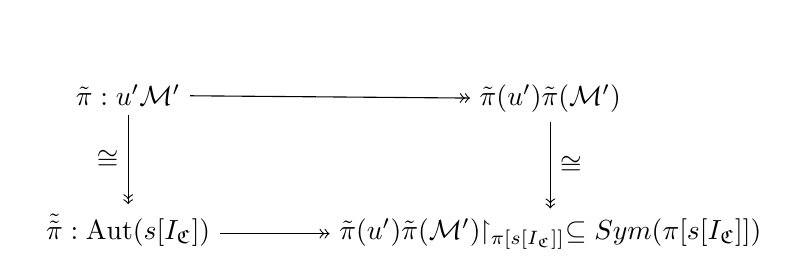
\begin{tikzpicture}\label{diagram pi}
        \matrix (m) [matrix of math nodes,row sep=3em,column sep=4em,minimum width=2em]
  {
     \Tilde{\pi}:u'\mathcal{M}' & \Tilde{\pi}(u')\Tilde{\pi}(\mathcal{M}') \\
     \Tilde{\Tilde{\pi}}:\aut(s[I_\C]) & \Tilde{\pi}(u')\Tilde{\pi}(\mathcal{M}')\!\!\upharpoonright_{\pi[s[I_\C]]} \subseteq Sym(\pi[s[I_\C]]) \\};
  \path[-stealth]
    (m-1-1) edge [->>] node [left] {$\cong$} (m-2-1)
            edge [->>] %node [below] {$\mathcal{B}_t$} 
            (m-1-2)
    (m-2-1.east|-m-2-2) edge [->>] %node [below] {$\mathcal{B}_T$}
            %node [above] {$\exists$} 
            (m-2-2)
    (m-1-2) edge [->>]  node [right] {$\cong$} (m-2-2);
            %edge [dashed,-] (m-2-1);
    \end{tikzpicture}
  \end{minipage}
  \begin{minipage}[c]{0.1\textwidth}
    \hfill (1) 
  \end{minipage}


    where:
    \begin{itemize}
        \item $\aut(s[I_\C])$ is the group of automorphisms in the infinitary definability patterns language.
        \item The map $\Tilde{\pi}$ is given by Fact \ref{epimorphism semigroup to group}.
        \item The isomorphism on the left is given by Proposition \ref{group isomorphism delta} and the fact that $s[I_\C]=\Image(u')$.
        \item The isomorphism on the right is given by Fact \ref{restrictio to image is monomorphism}.
        \item The map $\Tilde{\Tilde{\pi}}:\aut(s[I_\C]) \to Sym(\pi[s[I_\C]])$ is given by $\Tilde{\Tilde{\pi}}(\sigma)(\pi(x)):=\pi(\sigma(x))$ (which is the composition of the inverse of the left side isomorphism, the map $\tilde{\pi}$ and the right side isomorphism).
    \end{itemize}

    Similarly, $\rho: S_X(\C)\to S_X(\C)/F $ induces the following functions:
    
      \begin{minipage}[c]{0.8\textwidth}
              \hfill
        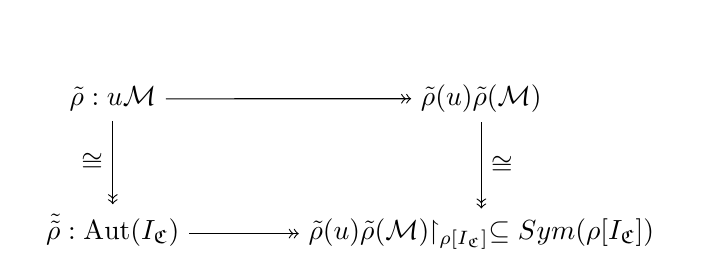
\begin{tikzpicture} \label{diagram rho}
        \matrix (m) [matrix of math nodes,row sep=3em,column sep=4em,minimum width=2em]
  {
     \Tilde{\rho}:u\mathcal{M} & \Tilde{\rho}(u)\Tilde{\rho}(\mathcal{M}) \\
     \Tilde{\Tilde{\rho}}:\aut(I_\C) & \Tilde{\rho}(u)\Tilde{\rho}(\mathcal{M})\!\!\upharpoonright_{\rho[I_\C]}\subseteq Sym(\rho[I_\C]) \\};
  \path[-stealth]
    (m-1-1) edge [->>] node [left] {$\cong$} (m-2-1)
            edge [->>] %node [below] {$\mathcal{B}_t$} 
            (m-1-2)
    (m-2-1.east|-m-2-2) edge [->>] %node [below] {$\mathcal{B}_T$}
            %node [above] {$\exists$} 
            (m-2-2)
    (m-1-2) edge [->>]  node [right] {$\cong$} (m-2-2);
            %edge [dashed,-] (m-2-1);
    \end{tikzpicture}
  \end{minipage}
  \begin{minipage}[c]{0.1\textwidth}
    \hfill (2) 
  \end{minipage}
  
 where:
 \begin{itemize}
     \item  $\aut(I_\C)$ is the group of automorphisms in the infinitary definability patterns language.
     \item The map $\Tilde{\rho}$ is given by Fact \ref{epimorphism semigroup to group}.
    \item The isomorphism on the left is given by Proposition \ref{group isomorphism delta}.
    \item The isomorphism on the right is given by Fact \ref{restrictio to image is monomorphism}.
    \item The map $\Tilde{\Tilde{\rho}}:\aut(I_\C) \to Sym(\rho[I_\C])$ is given by $\Tilde{\Tilde{\rho}}(\sigma)(\rho(x)):=\rho(\sigma(x))$ (which is the composition of the inverse of the left side isomorphism, the map $\tilde{\rho}$ and the right side isomorphism).
 \end{itemize}

 Since the map $r:s[I_\C]\to I_\C$ is an isomorphism in the infinitary patterns language, it induces an isomorphism $$\overline{r}: \aut(s[I_\C])\to \aut(I_\C)$$ given by $\overline{r}(\sigma)(r(p)):=r(\sigma(p))$. Our goal is then to prove that there exists an isomorphism $f$ such that the diagram below commutes:
   \begin{center}
        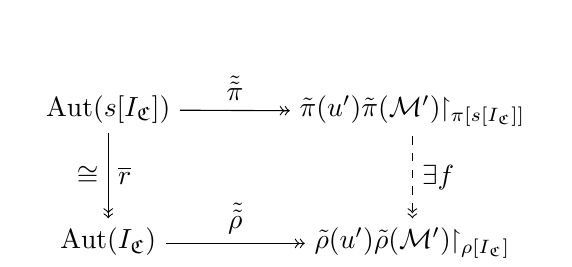
\begin{tikzpicture}
        \matrix (m) [matrix of math nodes,row sep=3em,column sep=4em,minimum width=2em]
  {
     \aut(s[I_\C]) & \Tilde{\pi}(u')\Tilde{\pi}(\mathcal{M}')\!\!\upharpoonright_{\pi[s[I_\C]]} \\
     \aut(I_\C) & \Tilde{\rho}(u')\Tilde{\rho}(\mathcal{M}')\!\!\upharpoonright_{\rho[I_\C]} \\};
  \path[-stealth]
    (m-1-1) edge [->>] node [left] {$\cong$} node [right] {$\overline{r}$} (m-2-1)
            edge [->>] node [above] {$\Tilde{\Tilde{\pi}}$} 
            (m-1-2)
    (m-2-1.east|-m-2-2) edge [->>]  node [above] {$\Tilde{\Tilde{\rho}}$}
            %node [above] {$\exists$} 
            (m-2-2)
    (m-1-2) edge [->>] [dashed] node [right] {$\exists f$ } 
    (m-2-2);
            %edge [dashed,-] (m-2-1);
    \end{tikzpicture}
\end{center}

We first show that a function $f$ such that the above diagram commutes exists. It is enough to show $\ker(\Tilde{\Tilde{\pi}})\subseteq \ker(\Tilde{\Tilde{\rho}}\circ \overline{r})$. Note that $\sigma\in \ker(\Tilde{\Tilde{\pi}})$ if and only if for every $p\in s[I_\C]$ we have that $\sigma(p)F' p$. Take an arbitrary $\sigma\in \ker(\Tilde{\Tilde{\pi}})$. By compatibility of $F'$ and F, $\sigma(p)F' p$ implies $ r(\sigma(p))F r(p)$. Hence, for every $p\in s[I_\C]$ we have $\overline{r}(\sigma)(r(p))F r(p)$. Therefore, $\overline{r}(\sigma)$ is in $\ker(\Tilde{\Tilde{\rho}})$ and $\sigma$ is in $\ker(\Tilde{\Tilde{\rho}}\circ \overline{r})$.

To see that $f$ is an isomorphism, it is enough to show that $\ker(\Tilde{\Tilde{\pi}})\supseteq \ker(\Tilde{\Tilde{\rho}}\circ \overline{r}).$ Take an arbitrary $\sigma\in \ker(\Tilde{\Tilde{\rho}}\circ \overline{r})$. Then, for every $p\in s[I_\C]$ we have that $r(\sigma(p))F r(p)$. \begin{claim}
    $r(\sigma(p))F r(p)$ implies $\sigma(p)F' p$.
\end{claim}
\begin{proof}[Proof of claim]
    By compatibility of $F'$ and $F$, there are $s_1,s_2\in S_X(\C')$ such that $r(s_1)=r(\sigma(p))$, $r(s_2)=r(p)$ and $s_1F' s_2$. At the same time, since $p,\sigma(p)\in s[I_\C]$, there are $i,j<\mu$ such that \begin{align*}
       \sigma(p)=p_i' &\wedge p=p_j';\\
        r(\sigma(p))=p_i &\wedge r(p)=p_j.        
    \end{align*}
    Hence, $c(s_1,s_2)\supseteq c(r(s_1),r(s_2))=c(r(\sigma(p)),p)=c(\sigma(p),p)$. Thus, there is $\eta\in E(S_X(\C'))$ such that $$\eta(s_1,s_2)=(\sigma(p),p).$$
    Therefore, since $F'$ is $\aut(\C')$-invariant and closed, $\sigma(p)F' p$.
\end{proof}
By the claim and the above description of $\ker(\Tilde{\Tilde{\pi}})$, we get that $\sigma\in \ker(\Tilde{\Tilde{\pi}})$.


Moreover, $f$ is a homeomorphism. To see this, note the following:
\begin{itemize}
    \item $\tilde{\tilde{\pi}}$ and $\tilde{\tilde{\rho}}$ are topological quotient maps (with the typologies on the right hand sides of the diagram induced by the $\tau$-topologies via the right vertical isomorphisms)
    \item $\bar r$ is a topological isomorphism.
\end{itemize}
The fact that  $\tilde{\tilde{\pi}}$ and $\tilde{\tilde{\rho}}$ are topological quotient maps follows from the fact that in their corresponding diagrams \hyperref[diagram pi]{(1)} and \hyperref[diagram rho]{(2)}, the upper horizontal maps are topological quotient maps by Fact \ref{epimorphism semigroup to group} and the left vertical maps are topological isomorphisms by Fact \ref{delta is homeomorphism}. The fact that $\bar r$ is a homeomorphism follows trivially by the definition of the ipp-topology and the fact that $\bar r$ is induced by an isomorphism of infinitary definability patterns structures.
\end{proof}



\section{Applications to tame, stable, NIP and WAP context}\label{section: nip stable tame wap}

In this section, we present several equivalence relations that are compatible, allowing us to use Theorem \ref{compatible implies absolute} to obtain absoluteness of their Ellis groups. For the notation used in this section, see Remark \ref{remark: pist and piNIP} and the comments following it. %We will assume that $\C$ is $\aleph_0$-saturated and strongly $\aleph_0$-homogeneous.

%Recall that $E^{\textrm{st}}_{\emptyset}$ is the finest $\emptyset$-type-definable equivalence relation on $X$ with stable quotient and $E^{\textrm{NIP}}_{\emptyset}$ is the finest $\emptyset$-type-definable equivalence relation on $X$ with NIP quotient. We denote by $E'^{\textrm{st}}_{\emptyset}$ the finest $\emptyset$-type-definable equivalence relation on $X(\C')$ with stable quotient and by $E'^{\textrm{NIP}}_{\emptyset}$ the finest $\emptyset$-type-definable equivalence relation on $X(\C')$ with NIP quotient.  Note that such $\emptyset$-type-definable equivalence relations on $\C$ exists because stability and NIP of hyperdefinable sets is closed under Cartesian products and taking type-definable subsets (see Remark \ref{finest eq exist for fixed param} for more details, and Proposition \ref{stable preserved product} and Corollary \ref{nip preserved product} for proofs).

%\begin{remark}
%    There is a type $\pi^{\textrm{st}}(x,y)$ over the empty set which for every monster model $\C$ (which is at least $(\aleph_0+|x|)$-saturated) defines the finest $\emptyset$-type-definable equivalence relation on $X \subseteq \C^{|x|}$ with stable quotient, denoted by $E^{\textrm{st}}_\emptyset$. Even if $\C$ is not sufficiently saturated, then by $E^{st}_\emptyset$ we mean $\pi^{st}(X(\C),X(\C))$. However, note that we do not need to talk about it, as we work with the equivalence relation $\tilde{E}^{\textrm{st}}_\emptyset$ on $S_X(\C)$ which is defined by $$p \tilde{E}^{\textrm{st}}_\emptyset q \iff (\exists a \models p,  b \models q) (\pi^{\textrm{st}}(a,b)).$$ %$\pi^{st}(x,y)$ working with realizations in a big monster model 
%    The same is true for $E^{\textrm{NIP}}_\emptyset$.
%\end{remark}

The following holds without any saturation assumptions on $\C$:
\begin{prop}
The equivalence relations $\tilde{E'}^{\textrm{st}}_\emptyset$ and $\tilde{E}^{\textrm{st}}_\emptyset$  are compatible.
\end{prop}

\begin{proof}
Let $\pi(x,y)$ be a partial type over $\emptyset$ (closed under conjunction) defining $E^{\textrm{st}}_\emptyset$. The same type defines $E'^{\textrm{st}}_\emptyset$. Recall also that $\tilde{E}^{\textrm{st}}_\emptyset$ is the equivalence relation on $S_X(\C)$ given by $$p \tilde{E}^{\textrm{st}}_\emptyset q \iff (\exists a \models p,  b \models q) (\pi(a,b)),$$ and $\tilde{E'}^{\textrm{st}}_\emptyset$ is the equivalence relation on $S_X(\C')$ given by $$p' \tilde{E'}^{\textrm{st}}_\emptyset q' \iff (\exists a' \models p',  b' \models q') (\pi(a',b')).$$

The goal is to prove that $r[\tilde{E'}^{\textrm{st}}_\emptyset] = \tilde{E}^{\textrm{st}}_\emptyset$.

$(\subseteq)$ Consider any $p',q' \in S_X(\C')$ with $p' \tilde{E'}^{\textrm{st}}_\emptyset  q'$. Then there are $a' \models p'$ and $b' \models q'$ such that $\pi(a',b')$. Hence, $a' \models r(p')$ and $b' \models r(b')$, and we get $r(p') \tilde{E}^{\textrm{st}}_\emptyset r(q')$.

$(\supseteq)$ Consider any $p,q \in S_X(\C)$ with $p \tilde{E}^{\textrm{st}}_\emptyset q$. The goal is to find some extensions $p',q' \in S_X(\C')$ of $p$ and $q$ respectively, satisfying $p' \tilde{E'}^{\textrm{st}}_\emptyset q'$. 

Take $a \models p$ and $b \models q$ such that $\pi(a,b)$. Let $\tp(a'b'/\C')$ be an heir extension of $\tp(ab/\C)$. We claim that $p':=\tp(a'/\C')$ and $q':=\tp(b'/\C)$ do the job. If not, then, by compactness, there are a formula $\varphi(x,y) \in \pi(x,y)$ and formulas $\psi_1(x,c') \in p'$ and $\psi_2(x,c') \in q'$ for which there are no $a''$ and $b''$ such that $\psi_1(a'',c') \wedge \psi_2(b'',c') \wedge \varphi(a'',b'')$ (here $\psi_i(x,x')$ is a formula without parameters and $c'$ is a tuple from $\C'$). Then 
$$\psi_1(x,c') \wedge \psi_2(y,c') \wedge \neg (\exists z)(\exists t)(\psi_1(z,c') \wedge \psi_2(t,c') \wedge \varphi(z,t)) \in \tp(a'b'/\C').$$
Since $\tp(a'b'/\C')$ is an heir extension of $\tp(ab/\C)$, there is $c \in \C$ such that 
$$\psi_1(x,c) \wedge \psi_2(y,c) \wedge \neg (\exists z)(\exists t)(\psi_1(z,c) \wedge \psi_2(t,c) \wedge \varphi(z,t)) \in \tp(ab/\C).$$
Taking $z:=a$ and $t:=b$, we get a contradiction with the fact that $\pi(a,b)$.
\end{proof}

From the previous proposition and Theorem \ref{compatible implies absolute}, we get the following immediate corollary (note the saturation assumption).

\begin{cor}
    The Ellis group of $S_X(\C)/\tilde{E}^{\textrm{st}}_\emptyset$ (treated as a topological group with the $\tau$-topology) does not depend on the choice of $\C$ as long as $\C$ is at least $\aleph_0$-saturated and strongly $\aleph_0$-homogeneous.
\end{cor}

Similarly, the following holds:

\begin{prop}
The equivalence relations $\tilde{E'}^{\textrm{NIP}}_\emptyset$ and $\tilde{E}^{\textrm{NIP}}_\emptyset$  are compatible.
\end{prop}

\begin{cor}
    The Ellis group of $S_X(\C)/\tilde{E}^{\textrm{NIP}}_\emptyset$ (treated as a topological group with the $\tau$-topology) does not depend on the choice of $\C$ as long as $\C$ is at least $\aleph_0$-saturated and strongly $\aleph_0$-homogeneous.
\end{cor}

Next, we will show that the same is true for the equivalence relations $\fwapp$ and $\fwap$ described in the preliminaries of this chapter. However, this time we will need $\C$ and $\C'$ to be at least $(\aleph_0+\lambda)^+$-saturated and strongly $(\aleph_0+\lambda)^+$-homogeneous (where lambda is such that $X\subseteq \C^\lambda$). In particular, if $\lambda$ is finite, then $\aleph_1$-saturated and strongly $\aleph_1$-homogeneous is enough. 
\begin{remark}
    For the proof of the next theorem, without loss of generality we will assume that $\C$ is $\C'$-small. This is because if the theorem holds under those assumptions, we can take a monster model $\C'' \succ \C'$ in which both $\C$ and $\C'$ are small, and apply the result to the pairs $\C'' \succ \C'$ and $\C'' \succ \C$. Namely, for $r_1\colon S_X(\C') \to S_X(\C)$, $r_2 \colon S_X(\C'') \to S_X(\C')$, and $r_3 \colon S_X(\C'') \to S_X(\C)$ being the restriction maps, the theorem yields $r_2[F_{\textrm{WAP}}'']=\fwapp$ and $r_3[F_{\textrm{WAP}}'']=\fwap$. As $r_1[r_2[F_{\textrm{WAP}}'']]=r_3[F_{\textrm{WAP}}'']$, we conclude that $r_1[\fwapp] =\fwap$.
\end{remark}


\begin{teor}\label{fwapp and fwap}
The equivalence relations $\fwapp$ and $\fwap$ are compatible as long as $\C$ and $\C'$ are at least $(\aleph_0+\lambda)^+$-saturated and strongly $(\aleph_0+\lambda)^+$-homogeneous.
\end{teor}

\begin{proof}
    We first prove that $\fwap\subseteq r[\fwapp]$. It suffices to show that $ r[\fwapp]$ is a closed $\aut(\C)$-invariant equivalence relation on $S_X(\C)$ with WAP quotient.
    \begin{itemize}
        \item Closedness is clear.
        \item Equivalence relation: Take $a=r(\alpha)$, $b=r(\beta)=r(\beta')$ and $c=r(\gamma)$ where $\alpha \fwapp \beta$ and $\beta' \fwapp \gamma$. Let $(p_i)_{i<\mu}$ be an enumeration of $S_X(\C)$ and $(a_i)_{i<\mu}$ be a sequence of realizations. Consider the type $p:=\tp((a_i)_{i<\mu}/\C)$ and let $\tp ((a'_i)_{i<\mu}/\C')=:p'$ be a strong heir extension of $p$ (see Definition \ref{strong heirs}). For each $i<\mu$ we denote $\tp(a_i'/\C')$ by $p_i'$. Obviously, $a=p_{i_1}$, $b=p_{i_2}$ and $c=p_{i_3}$ for some $i_1,i_2,i_3<\mu$.
        \begin{claim}
            $p'_{i_1}\fwapp p'_{i_2} \fwapp p'_{i_3}$.
        \end{claim}
        \begin{proof}[Proof of claim]
            Clearly, $r(p'_i)=p_i$ for all $i<\mu$. Since $p'$ is a strong heir of $p$ we have 
            \begin{align*}
                c(p'_{i_1},p'_{i_2})&=c(p_{i_1},p_{i_2})\subseteq c(\alpha,\beta)\\
                c(p'_{i_2},p'_{i_3})&=c(p_{i_2},p_{i_3})\subseteq c(\beta',\gamma).
            \end{align*}
            Thus, by Fact \ref{content and ellis semigroup}, \begin{align*}
                \exists \eta_1 \in E(S_X(\C'))&[ \eta_1 (\alpha, \beta)=(p'_{i_1},p'_{i_2})]\\
                \exists \eta_2 \in E(S_X(\C'))&[ \eta_2 (\beta', \gamma)=(p'_{i_2},p'_{i_3})].
            \end{align*}
            Since the relation $\fwapp$ is $\aut(\C')$-invariant, closed, and $ \alpha \fwapp \beta \wedge \beta'\fwapp \gamma $, we conclude that $p'_{i_1}\fwapp p'_{i_2} \fwapp p'_{i_3}$.
        \end{proof}
        By the claim, $p'_{1_1}\fwapp p'_{i_3}$, so $a=r(p'_{i_1}) r[\fwapp] r(p'_{i_3})=c$.
        \item $\aut(\C)$-invariant: Take an arbitrary $\sigma\in \aut(\C)$ and extend it to $\sigma'\in \aut(\C')$. Consider any $a,b\in S_X(\C)$ such that $a r[\fwapp] b$ and let $\alpha$, $\beta \in S_X(\C')$ be such that $r(\alpha)=a$, $r(\beta)=b$ and $\alpha \fwapp \beta$. Then, $$ \sigma(a)=\sigma(r(\alpha))=r(\sigma'(\alpha))r[\fwapp] r(\sigma'(\beta))=\sigma(r(\beta))=\sigma(b). $$
        \item $S_X(\C)/r[\fwapp]$ is WAP: Assume for a contradiction that there is a function $f \in C ( S_X(\C)/r[\fwapp] )$ which is not WAP. That is, there is a net $(\sigma_i)_{i\in \I}\subseteq \aut( \C)$ such that the functions $\sigma_if$ converge pointwise to some function $g\notin C ( S_X(\C)/r[\fwapp] )$. Note that $r^{-1}[r[\fwapp]]\supseteq \fwapp$ is a closed $\aut(\C'/\{ \C \})$-invariant equivalence relation on $S_X(\C')$ and $r$ induces a homeomorphism $$\Tilde{r}: \bslant{S_X(\C')}{r^{-1}[r[\fwapp]]}\to \bslant{S_X(\C)}{r[\fwapp]} $$ satisfying $$ \Tilde{r}\left(\sigma'\left(\bslant{p}{r^{-1}[r[\fwapp]]}\right) \right)=\sigma'\!\!\upharpoonright_\C\left(\bslant{r(p)}{r[\fwapp]}\right) $$ for all $\sigma'\in\aut(\C'/\{ \C\})$. In particular, we have a homomorphism
        $$ \left( \aut(\C'/\{ \C \}), \bslant{ S_X(\C')} {r^{-1}[r[\fwapp]]} \right) \to \left(\aut(\C), \bslant {S_X(\C)}{r[\fwapp]} \right) $$ given by $$ \sigma'\left( \bslant{p}{r^{-1}[r[\fwapp]]} \right)=\sigma'\!\!\upharpoonright_\C\left( \bslant{r(p)}{r[\fwapp]} \right). $$

        For every $i\in \I$ choose an extension $\sigma'_i\in \aut(\C'/\{ \C \})$ of $\sigma_i$. The above homeomorphism together with $f$ induce a function $f'\in C ( S( \C')/ r^{-1}[r[\fwapp]] )$ given by $$f'\left( \bslant{p}{r^{-1}[r[\fwapp]]} \right)=f\left( \bslant{r(p)}{r[\fwapp]} \right). $$ By construction, the net $(\sigma'_if')_{i\in I}$ converges pointwise to a function $$g'\notin C ( S( \C')/ r^{-1}[r[\fwapp]] ).$$ Hence, the flow $$ \left( \aut(\C'/\{ \C \}), \bslant{ S_X(\C')} {r^{-1}[r[\fwapp]]} \right)$$  is not WAP, which implies that $(\aut(\C'), S_X(\C')/\fwapp) $ is not WAP (because WAP is preserved under decreasing the acting group and under taking quotients of flows), a contradiction.
    \end{itemize}

    Now, we prove $\fwap\supseteq r[\fwapp]$. This is equivalent to $r^{-1}[\fwap]\supseteq \fwapp$. Note that $r^{-1}[\fwap]$ is a closed equivalence relation on $S_X(\C')$ but it might not be $\aut(\C')$-invariant. To solve it, we consider the equivalence relation $$ F:= \bigcap_{\sigma \in \aut(\C')} \sigma(r^{-1}[\fwap] ). $$ Then, it is enough to show that $F\supseteq \fwapp$ which is equivalent to the flow $$(\aut(\C'),  S_X(\C')/F)$$ being WAP.

    Assume for a contradiction that there is $f\in C(S_X(\C')/F)$ which is not WAP. Let $\overline{f}:S_X(\C')\to \R$ be given by $\overline{f}=f\circ \pi_F$, where $\pi_F:S_X(\C')\to S_X(\C')/F$ is the quotient map. Then, $\overline{f}\in C( S_X(\C'))$ and it is not a WAP function. By Fact \ref{double limit}, there are $(\sigma_n)_{n<\omega}\subseteq \aut(\C')$ and $(c'_m )_{m<\omega}\subset X(\C')$ such that \begin{equation}\label{dlp f}
        \lim_n\lim_m \sigma_n\overline{f} (\tp(c'_m/\C')) \neq \lim_m\lim_n \sigma_n\overline{f} (\tp(c'_m/\C'))
    \end{equation} where both limits exist. Note that here we are using that the types over $\C'$ of the elements of $X(\C')$ form a dense subset of $S_X(\C')$, which uses that $X$ lives on $\C'$-small (even $\C$-small) tuples.

    Consider the set $N:=\{ c'_m: m<\omega \}\cup \{ \sigma_n^{-1}(c'_m): m,n<\omega \}.$ By $(\aleph_0+\lambda)^+$-saturation of $\C$, we may assume that $N\subset \C$ (just find $\sigma\in\aut(\C)$ such that $\sigma[N]\subset \C$ and replace $N$ by $\sigma[N]$, $c'_m$ by $\sigma(c'_m)$ and $\sigma_n$ by $\sigma\circ \sigma_n$). Note that it might happen that none of the restrictions $\sigma_n\!\!\upharpoonright_\C$ is an automorphism of $\C$. However, for every $n<\omega$, by strong $(\aleph_0+\lambda)^+$-homogeneity of $\C$ (and strong $\lvert \C\rvert^+$-homogeneity of $\C')$, we can replace $\sigma_n$ by $\sigma'_n\in \aut(\C')$ so that $\sigma_n'^{-1}$ extends  $\sigma_n^{-1}\!\!\upharpoonright_{\{c'_m: m<\omega \}}$ and the restriction of $\sigma'_n$ to $\C$ is in $\aut(\C)$, so we may assume that, for every $n<\omega$, the restriction $\sigma_n\!\!\upharpoonright_\C$ is an element of $\aut(\C)$.

    Let $\mathcal{H}:= \{ p\in S_X(\C): p \text{ is invariant over } N \}$; we enumerate $\mathcal{H}= (p_i)_{i<\mu}$ and choose $a_i\models p_i$ for every $i<\mu$. Consider the type $p=\tp((a_i)_{i<\mu}/\C)$  and let $\tp ((a'_i)_{i<\mu}/\C')=:p'$ be a strong heir extension of $p$ in the language $\mL_N$ (it exists by $\aleph_0$-saturation of $\C$ in the language $\mL_N$ which follows from $\aleph_1$-saturation of $\C$ in the language $\mL$). We denote $\tp(a_i'/\C')$ by $p_i'$ for each $i<\mu$. Since $\tp(a_i/\C)$ is $N$-invariant, $p_i'$ is the unique $N$-invariant extension of $p_i$ to $\C'$. Hence, the set $\mathcal{H}':=\{p_i'\}_{i<\mu}$ is precisely the set of all types in $S_X(\C')$ invariant over $N$, so it is closed in $S_X(\C')$. 

    Now, we define $h:\mathcal{H} \to \R$ by $h(p_i):=\overline{f}(p_i')$. The function $h$ belongs to $C(\mathcal{H})$ since for each closed interval $I\subseteq \R$ we have that $h^{-1}[I]=r[\overline{f}^{-1}[I] \cap \mathcal{H}']$ is a closed subset of $S_X(\C)$. Note that for each $c'\in N$ and $i<\mu$, if $p_i=\tp(c'/\C)$ then $p_i'=\tp(c'/\C')$ and so \begin{equation}\label{6.2}
        \sigma_n(\overline{f}( \tp( c'_m/\C') ) = \overline{f}(\tp(\sigma_n^{-1}(c'_m)/\C'))=h(\tp(\sigma_n^{-1}(c'_m)/\C))= \sigma_n(h( \tp( c'_m/\C) ).
    \end{equation} Using \ref{dlp f} and the fact above we deduce:
    \begin{equation}\label{6.3}
        \lim_n\lim_m \sigma_n h (\tp(c'_m/\C)) \neq \lim_m\lim_n \sigma_n h (\tp(c'_m/\C))
    \end{equation} where both limits exist.

    \begin{claim}
        For $p_i,p_j \in\mathcal{H}$, if $p_i \fwap p_j$ then $h(p_i)=h(p_j)$.
    \end{claim}
    \begin{proof}[Proof of claim]
        We show that $p_i' F p_j'$. Choose an arbitrary $\sigma'\in\aut(\C')$. We have that $$ c(p_i,p_j)=c(p_i',p_j')=c(\sigma'(p_i'),\sigma'(p_j'))\supseteq c(r(\sigma'(p_i')),r(\sigma'(p_j'))) .$$ Hence, there is $\eta\in E(S_X(\C))$ such that $\eta(p_i,p_j)=(r(\sigma'(p_i')),r(\sigma'(p_j')))$, which implies that $ r(\sigma'(p_i')) \fwap r(\sigma'(p_j')) $ (because $\fwap$ is $\aut(\C)$-invariant and closed). We then have $\sigma'(p_i') r^{-1}[\fwap]\sigma'(p_j')$, and since $\sigma'$ was arbitrary, we conclude that $p_i' F p_j'$. Therefore, since $\overline{f}=f\circ\pi_F$, we obtain that $\overline{f}(p'_i)=\overline{f}(p'_j)$, so $h(p_i)=h(p_j)$.
    \end{proof}

    Clearly, $\mathcal{H}/\fwap$ is a closed subset of $S_X(\C)/\fwap$ and, by the claim, $h=g\circ \rho$ for some $g\in C(\mathcal{H}/\fwap )$ and $\rho: \mathcal{H} \to \mathcal{H}/\fwap$ the quotient map. Tietze's extension theorem yields a function $\overline{g}\in C(S_X(\C)/\fwap)$ extending $g$. By construction, this function satisfies \begin{equation}\label{6.4}
        \lim_n\lim_m \sigma_n\overline{g} \left(\bslant{\tp(c'_m/\C)}{\fwap}\right) \neq \lim_m\lim_n \sigma_n\overline{g} \left(\bslant{\tp(c'_m/\C)}{\fwap}\right)
    \end{equation} where both limits exist, which by Fact \ref{double limit} contradicts the fact that $S_X(\C)/\fwap$ is a WAP flow.
\end{proof}

From the previous theorem and Theorem \ref{compatible implies absolute}, the following corollary follows immediately.

\begin{cor}
    The Ellis group of $S_X(\C)/\fwap$ (treated as a topological group with the $\tau$-topology) does not depend on the choice of $\C$ as long as $\C$ is at least $(\aleph_0+\lambda)^+$-saturated and strongly $(\aleph_0+\lambda)^+$-homogeneous.
\end{cor}



Similarly, and under the same saturation assumptions, for the equivalence relations $\ftaa$ and $\fta$ we have the following:

\begin{teor}\label{ftaa and fta}
The equivalence relations $\ftaa$ and $\fta$ are compatible as long as $\C$ and $\C'$ are at least $(\aleph_0+\lambda)^+$-saturated and strongly $(\aleph_0+\lambda)^+$-homogeneous.
\end{teor}

\begin{proof}
    We first prove that $\fta\subseteq r[\ftaa]$. It suffices to show that $ r[\ftaa]$ is a closed $\aut(\C)$-invariant equivalence relation on $S_X(\C)$ with tame quotient. The fact that $r[\ftaa]$ is a closed $\aut(\C)$-invariant equivalence relation on $S_X(\C)$ follows by the same arguments as in the WAP context (see Theorem \ref{fwapp and fwap}).
    
    To show that $S_X(\C)/r[\ftaa]$ is tame, suppose for a contradiction that there is a function $f \in C ( S_X(\C)/r[\ftaa] )$ which is not tame. That is, there is a sequence $(\sigma_i)_{i<\omega}\subset\aut(\C)$ such that $(\sigma_i f)_{i<\omega}$ is an independent sequence. 
    Then we apply the corresponding part of the proof of Theorem \ref{fwapp and fwap}, replacing ``WAP" by ``tame" and noticing that by construction the sequence $(\sigma'_if')_{i<\omega}$ is independent, which leads to a contradiction.

    Now we prove $\fta\supseteq r[\ftaa]$. This is equivalent to $r^{-1}[\fta]\supseteq \ftaa$. We define a closed, $\aut(\C')$-invariant equivalence relation $$ F:= \bigcap_{\sigma \in \aut(\C')} \sigma(r^{-1}[\fta] ). $$ Then, it is enough to show that $F\supseteq \ftaa$ which is equivalent to the flow $$(\aut(\C'),  S_X(\C')/F)$$ being tame.

    Assume for a contradiction that there is $f\in C(S_X(\C')/F)$ which is not tame. Let $\overline{f}:S_X(\C')\to \R$ be given by $\overline{f}=f\circ \pi_F$. Then, $\overline{f}\in C( S_X(\C'))$ and it is not a tame function. That is, there exist $r<s\in \R$, $(\sigma_i)_{i<\omega}\subset\aut(\C')$ and $\{c'_{P,M}: P,M\subset_{fin} \omega \text{ disjoint} \}\subset X(\C')$ such that for any finite disjoint $P,M\subset \omega$ \begin{equation}\label{indep f}
        \models \{ \sigma_i\overline{f}(\tp(c'_{P,M}/\C'))<r: i\in P\} \cup \{\sigma_i\overline{f}(\tp(c'_{P,M}/\C'))>s: i\in M \}.
    \end{equation}
    The fact that we can choose $c'_{P,M}\in X(\C')$ follows from the fact that the types over $\C'$ of elements of $X(\C')$ form a dense subset of $S_X(\C')$ and the second part of Defnition \ref{defin: indep functons}.
    %By Grothendieck, there are $(\sigma_n)_{n<\omega}\subseteq \aut(\C)$ and $(c'_m )_{m<\omega}\subset \C'$ such that $$ \lim_n\lim_m \sigma_n\overline{f} (\tp(c'_m/\C')) \neq \lim_m\lim_n \sigma_n\overline{f} (\tp(c'_m/\C')) $$ where both limits exist.

    Consider the set $$N:=\{c'_{P,M}: P,M\subset_{fin} \omega \text{ disjoint} \}\cup \{\sigma_i^{-1}(c'_{P,M}): i<\omega, P,M\subset_{fin} \omega \text{ disjoint} \}.$$ By $(\aleph_0+\lambda)^+$-saturation of $\C$, applying an automorphism of $\C'$, we may assume that $N\subset \C$. Note that it might happen that none of the restrictions $\sigma_n\!\!\upharpoonright_\C$ is an automorphism of $\C$. However, for every $n<\omega$, by strong $(\aleph_0+\lambda)^+$-homogeneity of $\C$ (and strong $\lvert \C \rvert^{+}$-homogeneity of $\C'$), we can replace $\sigma_n$ by $\sigma'_n\in \aut(\C')$ so that $\sigma_n'^{-1}$ extends $\sigma_n^{-1}\!\!\upharpoonright_{\{c'_{P,M}: P,M\subset_{fin} \omega \text{ disjoint}\}}$ and the restriction of $\sigma'_n$ to $\C$ is in $\aut(\C)$, so we may assume that, for every $n<\omega$, $\sigma_n\!\!\upharpoonright_\C$ is an element of $\aut(\C)$.

    Let $\mathcal{H}:= \{ p\in S_X(\C): p \text{ is invariant over } N \}$, we enumerate $\mathcal{H}=( p_i)_{i<\mu}$ and choose $a_i\models p_i$ for every $i<\mu$.  Consider the type $p=\tp((a_i)_{i<\mu}/\C)$ and let $\tp ((a'_i)_{i<\mu}/\C')=:p'$ be a strong heir extension of $p$ in the language $\mL_N$, we denote $\tp(a_i'/\C')$ by $p_i'$ for each $i<\mu$. Since $\tp(a_i/\C)$ is $N$-invariant, $p_i'$ is the unique $N$-invariant extension of $p_i$ to $\C'$. Hence, the set $\mathcal{H}':=(p_i')_{i<\mu}$ is closed in $S_X(\C')$. 

    Then we apply the corresponding part of the proof of Theorem \ref{fwapp and fwap}, where the formulas \ref{6.2}, \ref{6.3} and \ref{6.4} are replaced by 
    $$ \sigma_n(\overline{f}( \tp( c'_{P,M}/\C') ) = \overline{f}(\tp(\sigma_n^{-1}(c'_{P,M})/\C'))=h(\tp(\sigma_n^{-1}(c'_{P,M})/\C))= \sigma_n(h( \tp( c'_{P,M}/\C) ),$$
    $$\models \{ \sigma_ih(\tp(c'_{P,M}/\C))<r: i\in P\} \cup \{\sigma_ih(\tp(c'_{P,M}/\C))>s: i\in M \}$$ and $$\models \{ \sigma_i\overline{g}(\tp(c'_{P,M}/\C))<r: i\in P\} \cup \{\sigma_i\overline{g}(\tp(c'_{P,M}/\C))>s: i\in M \},$$ respectively.
\end{proof}

Again, from the previous theorem and Theorem \ref{compatible implies absolute}, the following corollary follows immediately.

\begin{cor}
    The Ellis group of $S_X(\C)/\fta$ (treated as a topological group with the $\tau$-topology) does not depend on the choice of $\C$ as long as $\C$ is at least $(\aleph_0+\lambda)^+$-saturated and strongly $(\aleph_0+\lambda)^+$-homogeneous.
\end{cor}


\section{Stable vs WAP, and NIP vs tame}

In this last section, we will study the relation between the equivalence relations $\fta$ and $\fwap$ and the finest $\emptyset$-type-definable equivalence relations on $X$ with NIP and stable quotients, respectively. Assume that $\C$ is $(\aleph_0+\lambda)$-saturated and strongly $(\aleph_0+\lambda)$-homogeneous (where $X\subseteq \C^\lambda)$.


Let $E$ be a $\emptyset$-type-definable equivalence relation on $X$. By \ref{2.4} we know that the quotient $X/E$ is stable if and only if every $f\in \mathcal{F}_{X/E}$ is stable. The connection between stable theories and WAP flows is well known (see \cite{ben2016weakly}). This connection is still true for the hyperdefinable set $X/E$.

\begin{prop}\label{wap iff stable formula}
    Let $f(x,y)\in \mathcal{F}_{X/E}$, and let $b\in \C^{\lvert y \rvert}$. We denote by $f_b$ the function $f_b:S_{X/E}(\C)\to \R$ given by $f_b(p)=f(a,b)$ for any $a/E\models p$. Then the following are equivalent:
    \begin{enumerate}
        \item $f(x,y)$ is stable.
        \item For all $b\in \C^{\lvert y \rvert}$ the function $f_b$ is WAP.
    \end{enumerate}
\end{prop}
\begin{proof}
    $(1)\implies (2)$ If the function $f_b$ is not WAP, by Fact \ref{double limit}, there is a sequence $(a_n)_{n<\omega}\subset X$ and a sequence of automorphisms $(\sigma_m)_{m<\omega}\subset \aut(\C)$ such that $$\lim_m\lim_n f(a_n,\sigma_m(b))\neq \lim_n\lim_m f(a_n,\sigma_m(b)) .$$ Note that we are using that the realized types are dense in $S_X(\C)$.
    Assume, without loss of generality that for some $r<s\in \R$ we have $$\lim_m\lim_n f(a_n,\sigma_m(b))>s \text{ and } \lim_n\lim_m f(a_n,\sigma_m(b))<r.$$
    Let us denote $\sigma_m(b)$ by $b_m$. It is clear that we can choose a subsequence $(a_i',b_i')_{i<\omega}$ from $(a_n,b_n)_{n<\omega}$ such that $f(a'_i,b'_j)>s$ whenever $i>j$ and $f(a'_i,b'_j)<r$ whenever $i<j$. That is, the sequence $(a_i',b_i')_{i<\omega}$ witnesses unstability of the formula $f(x,y)$. 

    $(2)\implies (1)$ If $f(x,y)$ is unstable, we can find an indiscernible sequence $(a_i,b_i)_{i<\omega}$ with $a_i\in X$ and $b_i\in \C^{\lvert y \rvert}$ such that $f(a_i,b_j)\neq f(a_j,b_i)$ for some (all) $i<j$, By indiscernibility, for each $i<\omega$ there is $\sigma_i \in \aut(\C)$ such that $\sigma_i(b_0)=b_i$ and there exists $r<s\in \R$ such that $$f(a_i,b_j)=r<s=f(a_j,b_i)$$ for all $i<j$. Hence $f_{b_0}$ is not a WAP function.
\end{proof}

\begin{cor}\label{cor: stable iff wap}
    The flow $(\aut(\C), S_{X/E}(\C))$ is WAP if and only if $X/E$ is stable.
\end{cor}
\begin{proof}
    $(\Longrightarrow)$ By assumption, for any $f(x,y)\in\mathcal{F}_{X/E}$ and $b\in\C^{\lvert y\rvert}$, $f_b$ is WAP, so $f(x,y)$ is stable by Proposition \ref{wap iff stable formula}. Hence, $X/E$ is stable by Corollary \ref{2.4}.
    
    $(\Longleftarrow)$ By assumption and Corollary \ref{2.4}, every function $f(x,y)\in\mathcal{F}_{X/E}$ is stable, so for any $b\in \C^{\lvert y \rvert}$ the function $f_b$ is WAP by Proposition \ref{wap iff stable formula}. Thus, since by Proposition \ref{proposition: F_X/E separates points} the family of functions $\{ f_b: f\in \mathcal{F}_{X/E},b\in \C^{\lvert y \rvert}  \}$ separates points in $S_{X/E}(\C)$, we conclude that $(\aut(\C), S_{X/E}(\C))$ is WAP by Fact \ref{separating points: WAP}.
\end{proof}

%Note that given a $\emptyset$-type-definable equivalence relation $E$ on $\C$  we can define a $\emptyset$-type-definable equivalence relation $\Tilde{E}$ on $S_X(\C)$ given by $$ p\Tilde{E}q\iff \exists a\models p, b\models q \left( \tp(\bslant{a/E}{\C})=\tp(\bslant{b/E}{\C}) \right)$$ and $\Tilde{E}$ satisfies that $S_{\C/E}(\C)\cong S_\C(\C)/\Tilde{E}$.

Similarly, by Lemma \ref{IP_n hyperdef. set iif formulas} we know that the quotient $X/E$ has NIP if and only if every $f\in \mathcal{F}_{X/E}$ has NIP (see Definition \ref{defin: n-dep function/E} for $n=1$). The connection between NIP theories and tame flows is well known, it was first noticed independently in \cite{definably_Amenable_nip}, \cite{ibarlucia2016dynamical} and \cite{Khanaki2020-KHASTN} and further developed in \cite{Krupinski2018GaloisGA}. This connection is still true for the hyperdefinable set $X/E$.

\begin{prop}\label{tame iff nip formula}
    Let $f(x,y)\in \mathcal{F}_{X/E}$, and let $b\in \C^{\lvert y \rvert}$. We denote by $f_b$ the function $f_b:S_{X/E}(\C)\to \R$ given by $f_b(p)=f(a,b)$ for any $a/E\models p$. Then the following are equivalent:
    \begin{enumerate}
        \item $f(x,y)$ has NIP.
        \item For all $b\in \C^{\lvert y \rvert}$ the function $f_b$ is tame.
    \end{enumerate}
\end{prop}
\begin{proof}
    $(1)\implies (2)$. If $f_b$ is not tame for some $b\in \C^{\lvert y \rvert}$, then there is a sequence $(\sigma_i)_{i<\omega}\subset \aut(\C)$ such that the sequence of functions $(f(x,\sigma_i(b)))_{i<\omega}$ is independent on $X$, so $f$ has IP by compactness. %we construct a witness for $IP$ using the independent family $(f(x,\sigma_i(b)))_{i<\omega}$ and compactness.

    $(2)\implies (1)$. If $f(x,y)$ has $IP$, then we can find an element $a\in X$, an indiscernible sequence $(b_i)_{i<\omega}\subset \C^{\lvert y \rvert}$ and $r<s\in \mathbb{R}$ such that $f(a,b_i)<r$ if and only if $i$ is even and $f(a,b_i)>s$ if and only if $i$ is odd (see Lemma \ref{even odd nip}). By indiscernibility, for each $i<\omega$ there is $\sigma_i \in \aut(\C)$ such that $\sigma_i(b_0)=b_i$. Hence, $f_{b_0}$ is not a tame function because the sequence $(f(x,b_i))_{i<\omega}$ is independent.
\end{proof}

\begin{cor}\label{cor: nip iff tame}
    The flow $(\aut(\C), S_{X/E}(\C))$ is tame if and only if $X/E$ is NIP.
\end{cor}
\begin{proof}
    $(\Longrightarrow)$ By assumption, for any $f(x,y)\in\mathcal{F}_{X/E}$ and $b\in\C^{\lvert y\rvert}$, $f_b$ is tame, so $f(x,y)$ has NIP by Proposition \ref{tame iff nip formula}. Hence, $X/E$ has NIP by Lemma \ref{IP_n hyperdef. set iif formulas}.
    
    $(\Longleftarrow)$ By assumption and Lemma \ref{IP_n hyperdef. set iif formulas}, every function $f(x,y)\in\mathcal{F}_{X/E}$ has NIP, so for any $b\in \C^{\lvert y \rvert}$ the function $f_b$ is tame by Proposition \ref{tame iff nip formula}. Thus, since by Proposition \ref{proposition: F_X/E separates points} the family of functions $\{ f_b: f\in \mathcal{F}_{X/E},b\in \C^{\lvert y \rvert}  \}$ separates points in $S_{X/E}(\C)$, we conclude that $(\aut(\C), S_{X/E}(\C))$ is tame by Fact \ref{separating points: tame}.
    %$(2)\iff (3)$ holds by Proposition \ref{2.3}, Lemma \ref{IP_n hyperdef. set iif formulas} and Fact \ref{separating points: tame} since these results imply that the family $\{ f_b: f\in \mathcal{F}_{X/E},b\in \C^{\lvert y \rvert}  \}$ separates points and every function contained in it is tame.
\end{proof}

%Recall that $E^{\textrm{st}}_{\emptyset}$ is the finest $\emptyset$-type-definable equivalence relation on $\C$ with stable quotient, and $E^{\textrm{NIP}}_{\emptyset}$ is the finest $\emptyset$-type-definable equivalence relation on $\C$ with NIP quotient (which always exist).
Below we will use the notation introduced in Remark \ref{remark: pist and piNIP} and the comments following it. Note that, while a $\emptyset$-type-definable equivalence relation on $X$ induces a closed $\aut(\C)$-invariant equivalence relation on $S_X(\C)$, the converse is not true. Namely, not every closed $\aut(\C)$-invariant equivalence relation on $S_X(\C)$ is created this way. In the case of $\Tilde{E}^{\textrm{WAP}}_{\emptyset}$ and $\Tilde{E}^{\textrm{NIP}}_{\emptyset}$, by Corollaries \ref{cor: stable iff wap} and \ref{cor: nip iff tame}, we get that $S_X(\C)/\Tilde{E}^{\textrm{st}}_{\emptyset}$ is a WAP flow and $S_X(\C)/\Tilde{E}^{\textrm{NIP}}_{\emptyset}$ is a tame flow. However, the next proposition shows that $\Tilde{E}^{\textrm{st}}_{\emptyset}$ is may not be equal to $\fwap$ and $\Tilde{E}^{\textrm{NIP}}_{\emptyset}$  may not be equal to $\fta$.

\begin{prop}\label{fwap strictly finer}
    Assume that $X$ is an $\emptyset$-type-definable subset of $\C^\lambda$, and $\C$ is $(\aleph_0+\lambda)$-saturated and strongly $(\aleph_0+\lambda)$-homogeneous.
    \begin{enumerate}
        \item If $X$ is unstable, then $\fwap\subsetneq \Tilde{E}^{\textrm{st}}_{\emptyset}$.
        \item If $X$ has IP, then $\fta\subsetneq \Tilde{E}^{\textrm{NIP}}_{\emptyset}$.
    \end{enumerate}
\end{prop}
\begin{proof}
    The inclusions follow from the above observations that $S_X(\C)/\Tilde{E}^{\textrm{st}}_{\emptyset}$ is WAP and $S_X(\C)/\Tilde{E}^{\textrm{NIP}}_{\emptyset}$ is tame. It remains to show that $\fwap \neq \Tilde{E}^{\textrm{st}}_{\emptyset} $ and $\fta\neq \Tilde{E}^{\textrm{NIP}}_{\emptyset}$. We will prove the first thing; the proof of the second one is analogous.

Since $X$ is unstable, $E^{\textrm{st}}_\emptyset \ne  \;\,=$, so  $\tilde{E}^{\textrm{st}}_\emptyset$ glues some types in $S_X(\C)$ which are realized in $\C$.

On the other hand, define a closed equivalence relation $E$ on $S_X(\C)$ by $$pEq \iff p_= = q_=,$$ where $p_=$ and $q_=$ denote the restrictions of $p$ and $q$ to the empty language (so we allow only the equality relation). Let $S^=_{X}(\C)$ be the collection of all global types in the empty language of the elements from $X(\C')$, where $\C' \succ \C$ is a monster model of the original theory in which $\C$ is small. Then $S^=_{X}(\C) = \{\tp(a/\C)_=: a \in X\} \cup \{\textrm{the unique non-realized type}\}$ is a closed subset of $S^=_{\C}(\C)$ invariant under $\aut(\C)$. We also see that $S_X(\C)/E \cong S^=_{X}(\C)$ as $\aut(\C)$-flows.
As the theory of $\C$ in the empty language is stable, by Corollary \ref{cor: stable iff wap}, we get that $(\Sym(\C), S^=_{\C}(\C))$ is WAP. Hence, since WAP  is closed under decreasing the acting group and under taking subflows, $(\aut(\C), S^=_{X}(\C))$ is also WAP, and so is $(\aut(\C),S_X(\C)/E)$. Therefore, $\fwap \subseteq E$. Thus, since $E$ does not glue any realized types in $S_X(\C)$, neither does $\fwap$.

By the conclusions of the last two paragraphs, we conclude that $\fwap \ne \tilde{E}^{\textrm{st}}_\emptyset$.
\end{proof}

Although $\fwap$ and $\fta$ are almost always strictly finer than $\Tilde{E}^{\textrm{st}}_\emptyset$ and $\Tilde{E}^{\textrm{NIP}}_\emptyset$, the following question and its analog for the tame case remain open:

\begin{question}
    Are the Ellis groups of the flows $$(\aut(\C), S_X(\C)/\fwap)$$ and $$(\aut(\C), S_X(\C)/\Tilde{E}^{\textrm{st}}_\emptyset)$$ isomorphic?
\end{question}

Proposition \ref{fwap strictly finer} justifies our interest in $\fwap$ and $\fta$, because it suggests that the quotients by these equivalence relations should capture more information about the theory in question than the quotients by $\Tilde{E}^{\textrm{st}}_\emptyset$ and $\Tilde{E}^{\textrm{NIP}}_\emptyset$ while maintaining similar good properties (having in mind that WAP is a dynamical version of stability and tameness a dynamical version of NIP.





We prove that the properties of stability and NIP for hyperdefinable sets are preserved under (possibly infinite) Cartesian products and taking type-definable subsets. %We consider two $\emptyset$-type-definable sets $X'$ and $Y'$ and two $\emptyset$-type-definable equivalence relations $E$ and $F$ on $X'$ and $Y'$, respectively. We denote by $X$ the hyperdefinable set $X'/E$ and by $Y$ the hyperdefinable set $Y'/F$.

\begin{remark} \label{finest eq exist for fixed param}
    The above is enough to guarantee that for a fixed set of parameters $A$, an arbitrary intersection of $A$-type-definable equivalence relations $(E_i)_{i<\mu}$ with stable (respectively NIP) quotient on a type-definable set $X$ is an equivalence relation with stable (respectively NIP) quotient space. Moreover, the finest $A$-type-definable equivalence relation on $X$ with stable (respectively NIP) quotient always exists.
\end{remark}
\begin{proof}[Proof of the Remark]
     The hyperdefinable set $$\bslant{X}{\bigcap_{i<\mu}E_i}$$ can be naturally identified with a type-definable subset of $$\prod_{i<\mu}X/E_i.$$
     
     For the moreover part, consider the $A$-type-definable equivalence relation on $X$ defined as the intersection of all $A$-type-definable equivalence relations on $X$ with stable quotient.
\end{proof}

Clearly, taking type-definable subsets preserves both stability and NIP. Moreover, it is enough to have preservation of stability (respectively NIP) under products of two hyperdefinable sets since this case easily implies the general case.

For the remainder of the appendix, we consider two hyperdefinable sets $X/E$ and $Y/F$ where $X,Y\subset \C^\lambda$.

First, we prove it for stability. This was first stated in \cite[Remark 1.4]{MR3796277}, the proof we present comes from Anand Pillay.

\begin{prop}\label{stable preserved product}
    Let $X/E$ and $Y/F$ by stable hyperdefinable sets. Then, $X/E\times Y/F$ is a stable hyperdefinable set.
\end{prop}
\begin{proof}
    Suppose the conclusion does not hold. Let $(a_i,b_i,c_i)_{i<\omega}$ be an indiscernible sequence witnessing unstability of $X/E\times Y/F$. That is, for all $i,j<\omega$ $a_i\in X/E$, $b_i\in Y/F$, and $\tp(a_i,b_i,c_j)\neq \tp(a_j,b_j,c_i)$ for all $i\neq j$. Without loss of generality we may extend $\omega$ to a sufficiently big (to be able to extract indiscernibles) dense linear order $\I$ without endpoints.
    \begin{claim}
        $(c_j)_{j\neq 0}$ is indiscernible over $a_0$.
    \end{claim}
    \begin{proof}
        Note that it is enough to show that for any $i_1<\dots< i_n<0<i'<j_1< \dots < j_m$ $$c_{i_1},\dots c_{i_n},c_{j_1},\dots,c_{j_m} \equiv_{a_0}c_{i_1},\dots c_{i_{n-1}},c_{i'},c_{j_1},\dots,c_{j_m}.$$ Note also that the sequence $(a_i,c_i)_{i\in (i_{n-1},j_1)}$ is indiscernible over $$K:=\{c_{i_k}: k=1,\dots,n-1 \}\cup \{c_{j_k}: k=1,\dots,m \}.$$
        Suppose that the conclusion does not hold, this implies that for some setting as above, $$(c_{i_n},a_0)\not\equiv_K (c_{i'},a_0).$$ However, by indiscernibility of the original sequence, $(c_{i_n},a_0)\equiv_K (c_{0},a_{i'})$. Therefore, the sequence $(a_i,c_iK)_{i\in (i_{n-1},j_1)}$ contradicts the stability of $X/E$.
    \end{proof}
    \begin{claim}
        $\tp(a_0,b_0,c_j)$ is constant for $j>0$, $\tp(a_0,b_0,c_j)$ is constant for $j<0$, and $\tp(a_0,b_0,c_1)\neq \tp(a_0,b_0,c_{-1})$.
    \end{claim}
    \begin{proof}
        The fact that it is constant follows from the indiscernibility of the original sequence $(a_i,b_i,c_i)_{i\in \I}$. Moreover, we have $$\tp(a_0,b_0,c_{-1})\neq \tp(a_{-1},b_{-1},c_0)=\tp(a_0,b_0,c_{1}).$$ 
    \end{proof}

    From the claims it follows that for each $k\in\I$ and $i_1<\dots< i_n<k<j_1< \dots < j_n$ all distinct from $0$ there exists $b'_k\in Y/F$ such that \begin{align*}
    b'_kc_{i_1}\equiv_{a_0}\cdots\equiv_{a_0} b'_kc_{i_n}\equiv_{a_0}b_0c_{-1}\\
    b'_kc_{j_1}\equiv_{a_0}\cdots\equiv_{a_0} b'_kc_{j_n}\equiv_{a_0}b_0c_{1}.
\end{align*}
Thus, by compactness and extracting indiscernibles (see Fact \ref{extracting indiscernibles}), there is a sequence $(b''_i,c'_i)_{i<\omega}$ which is indiscernible over $a_0$ and $$\tp(b''_i,c'_j/a_0)\neq tp(b''_j,c'_i/a_0)$$ for all $i<j$, contradicting stability of $Y/F$.
\end{proof}


The next characterization of functions of the family $\mathcal{F}_{X/E}$ with NIP easily follows from Proposition \ref{Hyperim: IP_n iff encoding partite} and compactness.

\begin{lema}\label{even odd nip}
    For any $f(x,y)\in  \mathcal{F}_{X/E}$ the following are equivalent:
    \begin{enumerate}
        \item $f$ has IP.
        \item There exists an indiscernible sequence $(b_i)_{i<\omega}$, $a\in X$ and $r<s\in \R$ such that $$ f(a,b_i)<r\iff i \text{ is even} $$ $$f(a,b_i)>s\iff i \text{ is odd.}$$
    \end{enumerate}
\end{lema}



\begin{prop}\label{NIP formulas have limit}
    For every $f(x,y)\in\mathcal{F}_{X/E}$ and for every (infinite) linear order  $\I$ without maximal element, $f(x,y)$ has NIP if and only if for every indiscernible sequence $(b_i)_{i\in\I}$ and $a\in X$ there is $L\in\Image(f)\subseteq [r_1,r_2]$ (for some $r_1,r_2\in \R$) such that for every $\varepsilon>0$ there is $\I_0\subset \I$ an end segment satisfying $$ \lvert f(a,b_i)-L\rvert \leq \varepsilon$$ for all $i\in\I_0$ (i.e., $(f(a,b_i))_{i\in\I_0}$ converges to $L$).
\end{prop}
\begin{proof}
    
$(\Leftarrow)$ : Suppose $f(x,y)$ has IP. Let $(b_{i})_{i<\omega}$, $a\in X$, and $r< s \in[r_1,r_2]$ be such that \begin{align*}
    f(a,b_i)<r\iff i \text{ is even},\\
    f(a,b_i)>s\iff i \text{ is odd},
\end{align*}
(which exists by Lemma \ref{even odd nip}).

By compactness, we may extend the indiscernible sequence $(b_{i})_{i<\omega}$ to a new indiscernible sequence $(b'_{i})_{i\in \I}$ such that for any $i\in I$ if $f(a,b'_i)<r$ then $f(a,b'_{i+1})>s$ and vice versa.
By assumption, there is some $L$ to which $(f(a, b'_i))_{i\in \I}$ converges. % as $i$ goes to $\infty$. 
Let $0<\epsilon<\frac{s-r}{2}$. So there is an end segment $\I_0\subseteq \I$ such that for all $i\in \I_0$, $\left|f\left(a, b'_i\right)-L\right| \leq \epsilon$. Then, $$\left|f\left(a, b'_{i+1}\right)-L\right| \geq\left|f\left(a, b'_{i+1}\right)-f\left(a, b'_i\right)\right|-\left|f\left(a, b'_i\right)-L\right| \geq(s-r)-\epsilon \geq \frac{s-r}{2}>\epsilon.$$ Which is a contradiction.

$(\Rightarrow)$ : Let $(b_i: i \in\I)$ be an indiscernible sequence and $a\in X$, and suppose the conclusion does not hold for $(b_i: i \in\I)$ and $a$. That is, for every $L$ there is some $\epsilon>0$ such that for every  end segment $\I_{0} \subseteq \I$, there is $i \in \I_{0}$ such that $\left|f\left(a, b_i\right)-L\right|>\epsilon$.

%$\I$ does not have a maximal element (otherwise, it would converge to that). So ithout loss of generality, let $\I=\omega$. 
Since $\left\{f\left(a, b_i\right) \mid i\in \I \right\} \subset[r_1,r_2]$ and is infinite, it must have some accumulation point $L_{0}$. That is, for any $\epsilon >0$, for cofinally many $i\in \I$, we have $\left|f\left(a, b_i\right)-L_{0}\right| \leq \epsilon$.

Since $\left(f\left(a, b_i\right)\right)_{i\in \I}$ does not converge, there is $\epsilon>0$ such that for every end segment $\I_0\subseteq \I$, there is $j\in \I_0$ such that $\left|f\left(a, b_j\right)-L_{0}\right|>\epsilon$ and since \(L_{0}\) is an accumulation point, there are cofinally many $i\in \I_0$ for which we have \(\mid f\left(a, b_i\right)-\) $L_{0} \left\lvert\, \leq \frac{\epsilon}{2}\right.$

%There are infinitely many $j<\omega$ such that $\left|f\left(a_{j}, b\right)-L_{0}\right|>\epsilon$. In particular, 
Note that there must be either cofinally many $j\in \I$ such that $f\left(a, b_j\right)>L_{0}+\epsilon$ or cofinally many such that $f\left(a, b_j\right)<L_{0}-\epsilon$. We prove the result for the former case, the latter is analogous. Let $r=L_{0}+\frac{\epsilon}{2}$ and $s=L_{0}+\epsilon$. %In the former case, let $r=L_{0}+\frac{\epsilon}{2}$ and $s=L_{0}+\epsilon$. In the latter, let $r=L_{0}-\epsilon$ and $s=L_{0}-\frac{\epsilon}{2}$.

%Then we will define a subsequence \(\left(c_{i} \mid i<\omega\right)\) of \(\left(a_{i} \mid i<\omega\right)\) which will be indiscernible. 
We now construct an indiscernible sequence $(c_i)_{i<\omega}$ which, together with $a$, will witness that $f(x,y)$ has IP.
Let $c_{0}=b_{i}$ for some $b_{i}$ such that $f(a,b_i) \leq r$. This is possible since there are cofinally many \(b_{i}\) within \(\frac{\epsilon}{2}\) of \(L_{0}\). Let \(c_{1}=a_{j}\) with $j>i$ be such that $f(a,c_{1}) \geq s$. Similarly, this is possible since there are cofinally many \(j\in \I\) with \(b_{j}\) such that $ f\left(a, b_j\right)-L_{0}>\epsilon$. Iterating this process infinitely many times, we get a subsequence $(c_i)_{i<\omega}$ of $(b_i)_{i\in \I}$ which is indiscernible, %Continue this process, choosing \(c_{n}\) to be \(a_{i_{n}}\) such that if \(c_{n-1}=a_{i_{n-1}}\), then \(i_{n}>i_{n-1}\). This gives us an indiscernible sequence \(\left(c_{i} \mid i<\omega\right) . 
$f\left(a,c_{i}\right) \leq r$ if and only if \(i\) is even, and $f\left(a,c_{i}\right) \geq s$ if and only if \(i\) is odd. Thus, this sequence is as required (by Lemma \ref{even odd nip}).
\end{proof}

Using the previous results for functions of the family $\mathcal{F}_{X/E}$, we prove the following:

\begin{prop}\label{type stabilizes NIP}
    Let $X/E$ be a hyperdefinable set with $X\subseteq \C^\lambda$. If $X/E$ has NIP, for any indiscernible sequence $(b_i)_{i<(\lvert T\rvert +\lambda)^+}$ (of tuples from $\C$ of length at most $\lambda$) and any $a/E\in X/E$ there exists $\alpha < (\lvert T\rvert +\lambda)^+$ such that $(b_i)_{\alpha<i <(\lvert T\rvert +\lambda)^+}$ is indiscernible over $a/E$.
\end{prop}
\begin{proof}
    Assume the conclusion does not hold. Then, by Proposition \ref{proposition: F_X/E separates points}, for every $\alpha <(\lvert T\rvert +\lambda)^+$ we can find a function $f_\alpha(x,y_1,\dots,y_{k(\alpha)})\in \mathcal{F}_{X/E\times\C^{k(\alpha)\lambda}}$, two tuples of indices indices $\alpha<i_1<\dots<i_{k(\alpha)}<(\lvert T\rvert +\lambda)^+$ and $\alpha<j_1<\dots<j_{k(\alpha)}<(\lvert T\rvert +\lambda)^+$, and $r_\alpha<s_\alpha\in \mathbb{Q}$ satisfying $$\models f_\alpha(a,b_{i_1},\dots,b_{i_{k(\alpha)}})\leq r_\alpha \wedge f_\alpha(a,b_{j_1},\dots,b_{j_{k(\alpha)}})\geq s_\alpha.$$
    Moreover, the functions $f_\alpha$ can be chosen from a dense subset of $\mathcal{F}_{X/E }$ of cardinality $\lvert T \rvert +\lambda$ (see the proof of Corollary \ref{corollary: 2.4} for a detailed justification). Therefore, there is some function $f(x,y_1,\dots,y_k)$ and $r<s\in \mathbb{Q}$ such that $f_\alpha=f$, $r_\alpha=r$ and $s_\alpha=s$ for cofinally many values of $\alpha$. Then, we can construct inductively a sequence $\II=(i_1^l,\dots,i_k^l)_{l<\omega}$ such that $i_1^l<\dots<i_k^l<i_1^{l+1}$ for all $l<\omega$ and \begin{itemize}
        \item $\models f(a,b_{i^l_1},\dots,b_{i^l_{k}})<r$ if and only if $l$ is even,
        \item $\models f(a,b_{i^l_1},\dots,b_{i^l_{k}})>s$ if and only if $l$ is odd.
    \end{itemize}
    As the sequence $(b_{i_1^l},\dots, b_{i_k^l})_{l<\omega}$ is indiscernible, this implies that the function $f(x,y_1,\dots,y_k)$ has IP. By Lemma \ref{IP_n hyperdef. set iif formulas}, this is a contradiction with the assumption that $X/E$ has NIP.
\end{proof}
\begin{cor}\label{nip preserved product}
    Let $X/E$ and $Y/F$ be hyperdefinable sets with $NIP$. Then $X/E\times Y/F$ has NIP.
\end{cor}
\begin{proof}
    Let $(c_i)_{i<(\lvert T\rvert +\lambda)^+}$ be an arbitrary indiscernible sequence (of tuples from $\C$) and $(a,/E,b/F)$ an arbitrary pair from $X/E\times Y/F$. By applying Proposition \ref{type stabilizes NIP} twice, we get that there is $\alpha < (\lvert T\rvert +\lambda)^+$ such that $(c_i)_{\alpha <i<(\lvert T\rvert +\lambda)^+}$ is indiscernible over $(a/E,b/F)$.  Thus, the type of $(a/E,b/F,c_i)_{\alpha <i<(\lvert T\rvert +\lambda)^+}$ is constant. Since $a/E$, $b/F$ and the sequence $(c_i)_{i<(\lvert T\rvert +\lambda)^+}$ were arbitrary, Proposition \ref{NIP formulas have limit} implies that every $f(x,y,z)\in \mathcal{F}_{X/E\times Y/F}$ has NIP. Therefore, $X/E\times Y/F$ has NIP by Lemma \ref{IP_n hyperdef. set iif formulas}.
\end{proof}
To prove Fact \ref{delta is homeomorphism}, we need an auxiliary lemma. This result originally appeared in the first arXiv version of \cite{Krupiski2019RamseyTA}. We include a proof here for completeness.

\begin{lema}\label{tau closure equivalence}
    For any flow $(G,X)$, and $A\subseteq u\mathcal{M}$, the $\tau$-closure $\cl_\tau(A)$ can be described as the set of all limits contained in $u\mathcal{M}$ of nets $\eta_i a_i$ such that $\eta_i\in\mathcal{M}$, $a_i\in A$ and $\lim_i \eta_i =u$
\end{lema}
\begin{proof}
    Consider $a \in \cl_{\tau}(A)$. Then, by the definition of the $\tau$-topology, there are nets $(g_i)_i \subseteq G$ and $(a_i)_i \subseteq A$ such that $\lim_i g_i = u$ and $\lim_i g_i a_i = a$. Note that $u a_i = a_i$, as $a_i \in A \subseteq u\mathcal{M}$. Put $\eta_i := g_i u \in \mathcal{M}$ for all $i$. By left continuity, we have that $\lim_i \eta_i = \lim_i g_i u = (\lim_i g_i) u = u u = u$. Furthermore, $\lim_i \eta_i a_i = \lim_i g_i u a_i = \lim_i g_i a_i = a$.

Conversely, consider any $a \in u\mathcal{M}$ for which there are nets $(\eta_i)_i \subseteq \mathcal{M}$ and $(a_i)_i \subseteq A$ such that $\lim_i \eta_i = u$ and $\lim_i \eta_i a_i = a$. Since each $\eta_i$ can be approximated by elements of $G$ and the semigroup operation is left continuous, one can find a subnet $(a_j')_j$ of $(a_i)_i$ and a net $(g_j)_j \subseteq G$ such that $\lim_j g_j = u$ and $\lim_j g_j a_j' = a$, which means that $a \in \cl_{\tau}(A)$.
\end{proof}

\begin{proof}[\textbf{Proof of Fact \ref{delta is homeomorphism}}]
We first show that $\delta$ is continuous. Consider an arbitrary closed set $F_{\bar{\varphi}, \bar{p},\bar{q}, r}$ and take $\eta \in \cl_\tau(\delta^{-1}[F_{\bar{\varphi}, \bar{p},\bar{q}, r}])$. Choose some nets $(\sigma_i)$ in $\aut(\C)$ and $(\eta_i)$ in $\delta^{-1}[F_{\bar{\varphi}, \bar{p},\bar{q}, r}]$ such that $\lim \sigma_i = u$ and $\lim \sigma_i\eta_i= \eta$. 

Suppose for a contradiction that $ \eta \notin \delta^{-1}[F_{\bar{\varphi}, \bar{p},\bar{q}, r}]$, i.e. $\neg R_{\bar{\varphi}, r}(\eta(\bar{p}),q)$. Then there is $b \models r(y)$ such that $$\varphi_1(x,y) \in \eta(p_1), \dots, \varphi_m(x,b) \in \eta(p_m)$$ and $$\varphi_{m+1}(x,b) \in q_1, \dots, \varphi_{m+n}(x,b) \in q_{n}.$$ Since $\lim \sigma_i = u$ and $\lim \sigma_i\eta_i= \eta$, there exists a natural number $N$ such that for all $i>N$ we have $\neg R_{\bar{\varphi}, r}(\eta_i(\bar{p}),\bar{q})$, a contradiction with the choice of $\eta_i$.

Next, we show the continuity of $\delta^{-1}$. Consider an arbitrary $\eta \in u\mathcal{M}$ and a basis of open neighborhoods of $\delta(\eta)$ consisting of all open neighborhoods of $\delta(\eta)$ of the form $U_{\bar{\varphi}, \bar{p},\bar{q}, r}$, where $U_{\bar{\varphi}, \bar{p},\bar{q}, r}$ is the complement of $F_{\bar{\varphi}, \bar{p},\bar{q}, r}$. Let $I$ consist of all tuples $(\bar{\varphi}, \bar{p},\bar{q}, r, b)$, where the tuples $(\bar{\varphi}, \bar{p},\bar{q}, r)$ have the form described above and $b$ is any tuple realizing $r$ and such that
$$\varphi_1(x,b) \in \delta(\eta)(p_1),\dots, \varphi_m(x,b) \in \delta(\eta)(p_m),
\varphi_{m+1}(x,b) \in q_1,\dots, \varphi_{m+n}(x,b) \in q_n.$$


Order $I$ by:
$(\bar{\varphi}(x,y), \bar{p},\bar{q}, r(y),b) \leq (\bar{\varphi}'(x,z), \bar{p}',\bar{q}', r'(z),b')$ if $y \subseteq z$, $r' |_y=r$, $b'|_y=b$, $m:=|\bar{p}| \leq |\bar{p}'|=:m'$ and $n:=|\bar{q}| \leq |\bar {q}'|=:n'$, and there exists an injection $$\sigma \colon \{1,\dots,m+n\} \to \{1,\dots,m'+n'\}$$ such that $\sigma[\{1,\dots,m\}] \subseteq \{1,\dots,m'\}$, $\sigma[\{m+1,\dots,m+n\}] \subseteq \{m'+1,\dots,m'+n'\}$ and:
\begin{enumerate}
    \item $\varphi_j = \varphi'_{\sigma(j)}$  for all $j \leq m+n$,
    \item $p_j = p'_{\sigma(j)}$ for all $j \leq m$,
    \item $q_{m+j}=q'_{\sigma(m+j)}$ for all $j \leq n$.
\end{enumerate}
It is easy to check that $(I, \leq)$ is a directed set. For $i =(\bar{\varphi}, \bar{p},\bar{q}, r, b) \in I$ by $U_i$ we mean $U_{\bar{\varphi}, \bar{p},\bar{q}, r}$, clearly $i \leq i'$ implies $U_i' \subseteq U_i$.

It suffices to show that for any net $(\eta_k)_{k \in K}$ in $u\mathcal{M}$ such that $\lim_k \delta(\eta_k) = \delta(\eta)$ we have $\tau-\lim_k \eta_k =\eta$. For that it is enough to show that for any subnet $(\rho_j)_{j \in J}$ of $(\eta_k)_{k \in K}$ we have that $\eta$ is in the $\tau$-closure of $(\rho_j)_{j \in J}$.

Since $\lim_j \delta(\rho_j) = \delta(\eta)$ for every $i \in I$ there exists $j_i \in J$ such that $\delta(\rho_{j_i}) \in U_i$. Writing $i=(\bar{\varphi}, \bar{p},\bar{q}, r,b)$, we have $b_i \models r$ such that 
%$$(*)\;\;\;\;\;\;\; \varphi_1(x,b_i) \in \delta(\rho_{j_i})(p_1), \dots,  \varphi_m(x,b_i) \in \delta(\rho_{j_i})(p_m), 
%\varphi_{m+1}(x,b_i) \in q_1, \dots , \varphi_{m+n}(x,b_i) \in q_n.$$
\begin{equation}\tag{$\star$}
\begin{split}
    \varphi_1(x,b_i) \in \delta(\rho_{j_i})(p_1), \dots,  \varphi_m(x,b_i) \in \delta(\rho_{j_i})(p_m), \\
\varphi_{m+1}(x,b_i) \in q_1, \dots , \varphi_{m+n}(x,b_i) \in q_n.
\end{split}
\end{equation}

%\begin{align*}\tag{*}
%    &\varphi_1(x,b_i) \in \delta(\rho_{j_i})(p_1), \dots,  \varphi_m(x,b_i) \in \delta(\rho_{j_i})(p_m)\\
%    &\varphi_{m+1}(x,b_i) \in q_1, \dots , \varphi_{m+n}(x,b_i) \in q_n.
%\end{align*} 

On the other hand, by the definition of $I$, we have 
\begin{equation}\tag{$\star\star$}
    \begin{split}
        \varphi_1(x,b) \in \delta(\eta)(p_1),\dots, \varphi_m(x,b) \in \delta(\eta)(p_m),\\
        \varphi_{m+1}(x,b) \in q_1,\dots, \varphi_{m+n}(x,b) \in q_n.
    \end{split}
\end{equation}
%$$(**)\;\;\;\;\;\;\;\; \varphi_1(x,b) \in \delta(\eta)(p_1),\dots, \varphi_m(x,b) \in \delta(\eta)(p_m),
%\varphi_{m+1}(x,b) \in q_1,\dots, %\varphi_{m+n}(x,b) \in q_n$$

For each $i\in I$, choose $\sigma_i \in \aut(\C)$ such that $\sigma(b_i)=b$. % (it exists as $b$ and $b_i$ realizes $r$).
Then, by $(\star)$ we have $\varphi_{m+1}(x,b) \in \sigma_i(q_1), \dots , \varphi_{m+n}(x,b) \in \sigma_i(q_n)$.

Since for varying $i \in I$ the tuples $(q_1,\dots,q_n)$ range over all finite tuples from $\bar{\mathcal{J}}$ and the tuples $(\varphi_{m+1}(x,b),\dots, \varphi_{m+n}(x,b))$ over all possible tuples of formulas belonging, respectively, to $q_1,\dots,q_n$, we see that $\lim_i \sigma_i |_{\bar{\mathcal{J}}} = Id_{\bar{\mathcal{J}}}$. So $\lim_i \pi_{\sigma_i} \circ u = u$ and clearly $\pi_{\sigma_i} \circ u \in \mathcal{M}$. %(Here $\circ$ denotes the composition of functions; formally it should be $\pi_{\sigma_i}$ in palce of $\sigma_i$; bellow I may skip $\circ$.)

Also by $(\star)$, 
$\varphi_1(x,b) \in \sigma_i (\rho_{j_i} (p_1)), \dots,  \varphi_m(x,b) \in \sigma_i (\rho_{j_i}(p_m))$. Again, since for varying $i \in I$ the tuples $(p_1,\dots,p_m)$ range over all finite tuples from $\bar{\mathcal{J}}$ and the tuples $(\varphi_1(x,b),\dots, \varphi_m(x,b))$ over all possible tuples of formulas belonging, respectively, to $\eta(p_1),\dots,\eta(p_m)$, we see that $\lim_i (\pi_{\sigma_i} \circ \rho_{j_i}) |_{\bar{\mathcal{J}}} = \eta |_{\bar{\mathcal{J}}}$.
Since $\rho_{j_i} = \rho_{j_i}u=u\rho_{j_i}$ and $\eta=\eta u$, we get $\lim_i \sigma_i u \rho_{j_i} = \eta$.

Hence, by the previous two paragraphs and Lemma \ref{tau closure equivalence}, we conclude that $\eta$ is in the $\tau$-closure of $(\rho_j)_{j \in J}$ as required.
    
\end{proof}
% $ biblatex auxiliary file $
% $ biblatex bbl format version 3.1 $
% Do not modify the above lines!
%
% This is an auxiliary file used by the 'biblatex' package.
% This file may safely be deleted. It will be recreated as
% required.
%
\begingroup
\makeatletter
\@ifundefined{ver@biblatex.sty}
  {\@latex@error
     {Missing 'biblatex' package}
     {The bibliography requires the 'biblatex' package.}
      \aftergroup\endinput}
  {}
\endgroup

\datalist[entry]{anyt/global//global/global}
  \entry{1a7d4f5c-0dcd-37ec-b761-69bf07cad14f}{article}{}
    \name{author}{2}{}{%
      {{hash=AFG}{%
         family={Abramson},
         familyi={A\bibinitperiod},
         given={Fred\bibnamedelima G.},
         giveni={F\bibinitperiod\bibinitdelim G\bibinitperiod},
      }}%
      {{hash=HLA}{%
         family={Harrington},
         familyi={H\bibinitperiod},
         given={Leo\bibnamedelima A.},
         giveni={L\bibinitperiod\bibinitdelim A\bibinitperiod},
      }}%
    }
    \list{publisher}{1}{%
      {Association for Symbolic Logic}%
    }
    \strng{namehash}{AFGHLA1}
    \strng{fullhash}{AFGHLA1}
    \field{labelnamesource}{author}
    \field{labeltitlesource}{title}
    \field{labelalpha}{AH78}
    \field{sortinit}{A}
    \field{sortinithash}{A}
    \field{issn}{00224812}
    \field{number}{3}
    \field{pages}{572\bibrangedash 600}
    \field{title}{Models Without Indiscernibles}
    \field{volume}{43}
    \field{journaltitle}{The Journal of Symbolic Logic}
    \field{year}{1978}
  \endentry

  \entry{anderson2023fuzzy}{misc}{}
    \name{author}{1}{}{%
      {{hash=AA}{%
         family={Anderson},
         familyi={A\bibinitperiod},
         given={Aaron},
         giveni={A\bibinitperiod},
      }}%
    }
    \strng{namehash}{AA1}
    \strng{fullhash}{AA1}
    \field{labelnamesource}{author}
    \field{labeltitlesource}{title}
    \field{labelalpha}{And23}
    \field{sortinit}{A}
    \field{sortinithash}{A}
    \verb{eprint}
    \verb 2310.04393
    \endverb
    \field{title}{Fuzzy VC Combinatorics and Distality in Continuous Logic}
    \field{eprinttype}{arXiv}
    \field{eprintclass}{math.LO}
    \field{year}{2023}
  \endentry

  \entry{MR637201}{book}{}
    \name{author}{1}{}{%
      {{hash=ADL}{%
         family={Armacost},
         familyi={A\bibinitperiod},
         given={David\bibnamedelima L.},
         giveni={D\bibinitperiod\bibinitdelim L\bibinitperiod},
      }}%
    }
    \list{publisher}{1}{%
      {Marcel Dekker, Inc., New York}%
    }
    \strng{namehash}{ADL1}
    \strng{fullhash}{ADL1}
    \field{labelnamesource}{author}
    \field{labeltitlesource}{title}
    \field{labelalpha}{Arm81}
    \field{sortinit}{A}
    \field{sortinithash}{A}
    \field{isbn}{0-8247-1507-1}
    \field{pages}{vii+154}
    \field{series}{Monographs and Textbooks in Pure and Applied Mathematics}
    \field{title}{The structure of locally compact abelian groups}
    \field{volume}{68}
    \field{year}{1981}
  \endentry

  \entry{auslander1988minimal}{book}{}
    \name{author}{1}{}{%
      {{hash=AJ}{%
         family={Auslander},
         familyi={A\bibinitperiod},
         given={J.},
         giveni={J\bibinitperiod},
      }}%
    }
    \list{publisher}{1}{%
      {Elsevier Science}%
    }
    \strng{namehash}{AJ1}
    \strng{fullhash}{AJ1}
    \field{labelnamesource}{author}
    \field{labeltitlesource}{title}
    \field{labelalpha}{Aus88}
    \field{sortinit}{A}
    \field{sortinithash}{A}
    \field{isbn}{9780444704535}
    \field{number}{n.{\textordmasculine} 153}
    \field{series}{Minimal Flows and Their Extensions}
    \field{title}{Minimal Flows and Their Extensions}
    \field{year}{1988}
  \endentry

  \entry{Bodirsky_2015}{inbook}{}
    \name{author}{1}{}{%
      {{hash=BM}{%
         family={Bodirsky},
         familyi={B\bibinitperiod},
         given={Manuel},
         giveni={M\bibinitperiod},
      }}%
    }
    \list{publisher}{1}{%
      {Cambridge University Press}%
    }
    \strng{namehash}{BM1}
    \strng{fullhash}{BM1}
    \field{labelnamesource}{author}
    \field{labeltitlesource}{title}
    \field{labelalpha}{Bod15}
    \field{sortinit}{B}
    \field{sortinithash}{B}
    \field{booktitle}{Surveys in Combinatorics 2015}
    \field{pages}{1–48}
    \field{series}{London Mathematical Society Lecture Note Series}
    \field{title}{Ramsey classes: examples and constructions}
    \field{year}{2015}
  \endentry

  \entry{doi:10.1142/S0219061303000297}{article}{}
    \name{author}{1}{}{%
      {{hash=BYI}{%
         family={Ben-Yaacov},
         familyi={B\bibinithyphendelim Y\bibinitperiod},
         given={Itay},
         giveni={I\bibinitperiod},
      }}%
    }
    \strng{namehash}{BYI3}
    \strng{fullhash}{BYI3}
    \field{labelnamesource}{author}
    \field{labeltitlesource}{title}
    \field{labelalpha}{BY03}
    \field{sortinit}{B}
    \field{sortinithash}{B}
    \verb{doi}
    \verb 10.1142/S0219061303000297
    \endverb
    \field{number}{02}
    \field{pages}{163\bibrangedash 191}
    \field{title}{Simplicity in compact abstarct theories}
    \field{volume}{03}
    \field{journaltitle}{Journal of Mathematical Logic}
    \field{year}{2003}
  \endentry

  \entry{10.2178/jsl/1122038916}{article}{}
    \name{author}{1}{}{%
      {{hash=BYI}{%
         family={Ben-Yaacov},
         familyi={B\bibinithyphendelim Y\bibinitperiod},
         given={Itay},
         giveni={I\bibinitperiod},
      }}%
    }
    \list{publisher}{1}{%
      {Association for Symbolic Logic}%
    }
    \keyw{categoricity, compact abstract theories}
    \strng{namehash}{BYI3}
    \strng{fullhash}{BYI3}
    \field{labelnamesource}{author}
    \field{labeltitlesource}{title}
    \field{labelalpha}{BY05}
    \field{sortinit}{B}
    \field{sortinithash}{B}
    \verb{doi}
    \verb 10.2178/jsl/1122038916
    \endverb
    \field{number}{3}
    \field{pages}{829 \bibrangedash  860}
    \field{title}{{Uncountable dense categoricity in cats}}
    \field{volume}{70}
    \field{journaltitle}{Journal of Symbolic Logic}
    \field{year}{2005}
  \endentry

  \entry{ContVCclasses}{article}{}
    \name{author}{1}{}{%
      {{hash=BYI}{%
         family={Ben\bibnamedelima Yaacov},
         familyi={B\bibinitperiod\bibinitdelim Y\bibinitperiod},
         given={Ita\"{i}},
         giveni={I\bibinitperiod},
      }}%
    }
    \keyw{Indiscernibles; Dividing-lines; Combinatorics; Fraisse class;
  Complexity; Hierarchies}
    \strng{namehash}{BYI2}
    \strng{fullhash}{BYI2}
    \field{labelnamesource}{author}
    \field{labeltitlesource}{title}
    \field{labelalpha}{BY09}
    \field{sortinit}{B}
    \field{sortinithash}{B}
    \field{number}{1}
    \field{pages}{309\bibrangedash 333}
    \field{title}{Continuous and random Vapnik-Chervonenkis classes}
    \field{volume}{179}
    \field{journaltitle}{Israel Journal of Mathematics}
    \field{year}{2009}
  \endentry

  \entry{2010}{article}{}
    \name{author}{1}{}{%
      {{hash=BYI}{%
         family={Ben\bibnamedelima Yaacov},
         familyi={B\bibinitperiod\bibinitdelim Y\bibinitperiod},
         given={Itaï},
         giveni={I\bibinitperiod},
      }}%
    }
    \list{publisher}{1}{%
      {Cambridge University Press (CUP)}%
    }
    \strng{namehash}{BYI1}
    \strng{fullhash}{BYI1}
    \field{labelnamesource}{author}
    \field{labeltitlesource}{title}
    \field{labelalpha}{BY10}
    \field{extraalpha}{1}
    \field{sortinit}{B}
    \field{sortinithash}{B}
    \verb{doi}
    \verb 10.2178/jsl/1278682202
    \endverb
    \field{issn}{1943-5886}
    \field{number}{3}
    \field{pages}{817–840}
    \field{title}{Definability of groups in $\aleph_0$-stable metric
  structures}
    \field{volume}{75}
    \field{journaltitle}{The Journal of Symbolic Logic}
    \field{year}{2010}
  \endentry

  \entry{MR2723787}{article}{}
    \name{author}{1}{}{%
      {{hash=BYI}{%
         family={Ben\bibnamedelima Yaacov},
         familyi={B\bibinitperiod\bibinitdelim Y\bibinitperiod},
         given={Ita\"{i}},
         giveni={I\bibinitperiod},
      }}%
    }
    \strng{namehash}{BYI2}
    \strng{fullhash}{BYI2}
    \field{labelnamesource}{author}
    \field{labeltitlesource}{title}
    \field{labelalpha}{BY10}
    \field{extraalpha}{2}
    \field{sortinit}{B}
    \field{sortinithash}{B}
    \verb{doi}
    \verb 10.2178/jsl/1278682220
    \endverb
    \field{number}{3}
    \field{pages}{1111\bibrangedash 1136}
    \field{title}{Stability and stable groups in continuous logic}
    \field{volume}{75}
    \field{journaltitle}{J. Symbolic Logic}
    \field{year}{2010}
  \endentry

  \entry{ben2016weakly}{article}{}
    \name{author}{2}{}{%
      {{hash=BYI}{%
         family={Ben\bibnamedelima Yaacov},
         familyi={B\bibinitperiod\bibinitdelim Y\bibinitperiod},
         given={Ita{\"\i}},
         giveni={I\bibinitperiod},
      }}%
      {{hash=TT}{%
         family={Tsankov},
         familyi={T\bibinitperiod},
         given={Todor},
         giveni={T\bibinitperiod},
      }}%
    }
    \strng{namehash}{BYITT1}
    \strng{fullhash}{BYITT1}
    \field{labelnamesource}{author}
    \field{labeltitlesource}{title}
    \field{labelalpha}{BYT16}
    \field{sortinit}{B}
    \field{sortinithash}{B}
    \field{number}{11}
    \field{pages}{8267\bibrangedash 8294}
    \field{title}{Weakly almost periodic functions, model-theoretic stability,
  and minimality of topological groups}
    \field{volume}{368}
    \field{journaltitle}{Transactions of the American Mathematical Society}
    \field{year}{2016}
  \endentry

  \entry{MR2657678}{article}{}
    \name{author}{2}{}{%
      {{hash=BYI}{%
         family={Ben\bibnamedelima Yaacov},
         familyi={B\bibinitperiod\bibinitdelim Y\bibinitperiod},
         given={Ita\"{i}},
         giveni={I\bibinitperiod},
      }}%
      {{hash=UA}{%
         family={Usvyatsov},
         familyi={U\bibinitperiod},
         given={Alexander},
         giveni={A\bibinitperiod},
      }}%
    }
    \strng{namehash}{BYIUA1}
    \strng{fullhash}{BYIUA1}
    \field{labelnamesource}{author}
    \field{labeltitlesource}{title}
    \field{labelalpha}{BYU10}
    \field{sortinit}{B}
    \field{sortinithash}{B}
    \verb{doi}
    \verb 10.1090/S0002-9947-10-04837-3
    \endverb
    \field{number}{10}
    \field{pages}{5213\bibrangedash 5259}
    \field{title}{Continuous first order logic and local stability}
    \field{volume}{362}
    \field{journaltitle}{Trans. Amer. Math. Soc.}
    \field{year}{2010}
  \endentry

  \entry{casanovas2011simple}{book}{}
    \name{author}{1}{}{%
      {{hash=CE}{%
         family={Casanovas},
         familyi={C\bibinitperiod},
         given={E.},
         giveni={E\bibinitperiod},
      }}%
    }
    \list{publisher}{1}{%
      {Cambridge University Press}%
    }
    \strng{namehash}{CE1}
    \strng{fullhash}{CE1}
    \field{labelnamesource}{author}
    \field{labeltitlesource}{title}
    \field{labelalpha}{Cas11}
    \field{sortinit}{C}
    \field{sortinithash}{C}
    \field{isbn}{9780521119559}
    \field{series}{Lecture Notes in Logic}
    \field{title}{Simple Theories and Hyperimaginaries}
    \field{year}{2011}
  \endentry

  \entry{conant2021separation}{misc}{}
    \name{author}{2}{}{%
      {{hash=CG}{%
         family={Conant},
         familyi={C\bibinitperiod},
         given={Gabriel},
         giveni={G\bibinitperiod},
      }}%
      {{hash=HJ}{%
         family={Hanson},
         familyi={H\bibinitperiod},
         given={James},
         giveni={J\bibinitperiod},
      }}%
    }
    \strng{namehash}{CGHJ1}
    \strng{fullhash}{CGHJ1}
    \field{labelnamesource}{author}
    \field{labeltitlesource}{title}
    \field{labelalpha}{CH21}
    \field{sortinit}{C}
    \field{sortinithash}{C}
    \verb{eprint}
    \verb 2110.07763
    \endverb
    \field{title}{Separation for isometric group actions and hyperimaginary
  independence}
    \field{eprinttype}{arXiv}
    \field{eprintclass}{math.LO}
    \field{year}{2021}
  \endentry

  \entry{Chernikov2014OnN}{article}{}
    \name{author}{3}{}{%
      {{hash=CA}{%
         family={Chernikov},
         familyi={C\bibinitperiod},
         given={Artem},
         giveni={A\bibinitperiod},
      }}%
      {{hash=PD}{%
         family={Palac{\'i}n},
         familyi={P\bibinitperiod},
         given={Daniel},
         giveni={D\bibinitperiod},
      }}%
      {{hash=TK}{%
         family={Takeuchi},
         familyi={T\bibinitperiod},
         given={Kota},
         giveni={K\bibinitperiod},
      }}%
    }
    \strng{namehash}{CAPDTK1}
    \strng{fullhash}{CAPDTK1}
    \field{labelnamesource}{author}
    \field{labeltitlesource}{title}
    \field{labelalpha}{CPT14}
    \field{sortinit}{C}
    \field{sortinithash}{C}
    \field{pages}{195\bibrangedash 214}
    \field{title}{On n-Dependence}
    \field{volume}{60}
    \field{journaltitle}{Notre Dame J. Formal Log.}
    \field{year}{2014}
  \endentry

  \entry{definably_Amenable_nip}{article}{}
    \name{author}{2}{}{%
      {{hash=CA}{%
         family={Chernikov},
         familyi={C\bibinitperiod},
         given={Artem},
         giveni={A\bibinitperiod},
      }}%
      {{hash=SP}{%
         family={Simon},
         familyi={S\bibinitperiod},
         given={Pierre},
         giveni={P\bibinitperiod},
      }}%
    }
    \strng{namehash}{CASP1}
    \strng{fullhash}{CASP1}
    \field{labelnamesource}{author}
    \field{labeltitlesource}{title}
    \field{labelalpha}{CS18}
    \field{sortinit}{C}
    \field{sortinithash}{C}
    \verb{doi}
    \verb https://doi.org/10.1090/jams/896
    \endverb
    \field{pages}{609\bibrangedash 641}
    \field{title}{Definably amenable NIP groups}
    \field{volume}{31}
    \field{journaltitle}{J. Amer. Math. Soc.}
    \field{year}{2018}
  \endentry

  \entry{Chernikov2020HypergraphRA}{article}{}
    \name{author}{2}{}{%
      {{hash=CA}{%
         family={Chernikov},
         familyi={C\bibinitperiod},
         given={Artem},
         giveni={A\bibinitperiod},
      }}%
      {{hash=TH}{%
         family={Towsner},
         familyi={T\bibinitperiod},
         given={Henry},
         giveni={H\bibinitperiod},
      }}%
    }
    \strng{namehash}{CATH1}
    \strng{fullhash}{CATH1}
    \field{labelnamesource}{author}
    \field{labeltitlesource}{title}
    \field{labelalpha}{CT20}
    \field{sortinit}{C}
    \field{sortinithash}{C}
    \field{title}{Hypergraph regularity and higher arity VC-dimension}
    \field{volume}{abs/2010.00726}
    \field{journaltitle}{ArXiv}
    \field{year}{2020}
  \endentry

  \entry{Dobrowolski2021KimindependenceIP}{article}{}
    \name{author}{2}{}{%
      {{hash=DJC}{%
         family={Dobrowolski},
         familyi={D\bibinitperiod},
         given={Jan\bibnamedelima Cz.},
         giveni={J\bibinitperiod\bibinitdelim C\bibinitperiod},
      }}%
      {{hash=KM}{%
         family={Kamsma},
         familyi={K\bibinitperiod},
         given={Mark},
         giveni={M\bibinitperiod},
      }}%
    }
    \strng{namehash}{DJCKM1}
    \strng{fullhash}{DJCKM1}
    \field{labelnamesource}{author}
    \field{labeltitlesource}{title}
    \field{labelalpha}{DK21}
    \field{sortinit}{D}
    \field{sortinithash}{D}
    \verb{doi}
    \verb 10.2140/mt.2022.1.55
    \endverb
    \field{title}{Kim-independence in positive logic}
    \field{journaltitle}{Model Theory}
    \field{year}{2021}
  \endentry

  \entry{55bad191-0781-3b5e-a214-06bd2e8fc797}{article}{}
    \name{author}{2}{}{%
      {{hash=ER}{%
         family={Ellis},
         familyi={E\bibinitperiod},
         given={R.},
         giveni={R\bibinitperiod},
      }}%
      {{hash=NM}{%
         family={Nerurkar},
         familyi={N\bibinitperiod},
         given={M.},
         giveni={M\bibinitperiod},
      }}%
    }
    \list{publisher}{1}{%
      {American Mathematical Society}%
    }
    \strng{namehash}{ERNM1}
    \strng{fullhash}{ERNM1}
    \field{labelnamesource}{author}
    \field{labeltitlesource}{title}
    \field{labelalpha}{EN89}
    \field{sortinit}{E}
    \field{sortinithash}{E}
    \field{issn}{00029947}
    \field{number}{1}
    \field{pages}{103\bibrangedash 119}
    \field{title}{Weakly Almost Periodic Flows}
    \field{volume}{313}
    \field{journaltitle}{Transactions of the American Mathematical Society}
    \field{year}{1989}
  \endentry

  \entry{Guingona2019}{article}{}
    \name{author}{2}{}{%
      {{hash=GV}{%
         family={Guingona},
         familyi={G\bibinitperiod},
         given={Vincent},
         giveni={V\bibinitperiod},
      }}%
      {{hash=HCD}{%
         family={Hill},
         familyi={H\bibinitperiod},
         given={Cameron\bibnamedelima Donnay},
         giveni={C\bibinitperiod\bibinitdelim D\bibinitperiod},
      }}%
    }
    \keyw{Indiscernibles; Dividing-lines; Combinatorics; Fraisse class;
  Complexity; Hierarchies}
    \strng{namehash}{GVHCD1}
    \strng{fullhash}{GVHCD1}
    \field{labelnamesource}{author}
    \field{labeltitlesource}{title}
    \field{labelalpha}{GH19}
    \field{sortinit}{G}
    \field{sortinithash}{G}
    \verb{doi}
    \verb 10.1007/s00153-018-0635-2
    \endverb
    \field{number}{3-4}
    \field{pages}{289\bibrangedash 323}
    \field{title}{On positive local combinatorial dividing-lines in model
  theory}
    \field{volume}{58}
    \field{journaltitle}{Archive for Mathematical Logic}
    \field{year}{2019}
  \endentry

  \entry{gismatullin2020bohr}{article}{}
    \name{author}{3}{}{%
      {{hash=GJ}{%
         family={Gismatullin},
         familyi={G\bibinitperiod},
         given={Jakub},
         giveni={J\bibinitperiod},
      }}%
      {{hash=JG}{%
         family={Jagiella},
         familyi={J\bibinitperiod},
         given={Grzegorz},
         giveni={G\bibinitperiod},
      }}%
      {{hash=KK}{%
         family={Krupi\'{n}ski},
         familyi={K\bibinitperiod},
         given={Krzysztof},
         giveni={K\bibinitperiod},
      }}%
    }
    \strng{namehash}{GJJGKK1}
    \strng{fullhash}{GJJGKK1}
    \field{labelnamesource}{author}
    \field{labeltitlesource}{title}
    \field{labelalpha}{GJK22}
    \field{sortinit}{G}
    \field{sortinithash}{G}
    \verb{doi}
    \verb 10.1017/jsl.2022.10
    \endverb
    \field{pages}{to appear}
    \field{title}{Bohr Compactifications of Groups and Rings}
    \field{journaltitle}{J. Symb. Log.}
    \field{year}{2022}
  \endentry

  \entry{Glasner1976}{inbook}{}
    \name{author}{1}{}{%
      {{hash=GS}{%
         family={Glasner},
         familyi={G\bibinitperiod},
         given={Shmuel},
         giveni={S\bibinitperiod},
      }}%
    }
    \list{publisher}{1}{%
      {Springer Berlin Heidelberg}%
    }
    \strng{namehash}{GS1}
    \strng{fullhash}{GS1}
    \field{labelnamesource}{author}
    \field{labeltitlesource}{title}
    \field{labelalpha}{Gla76}
    \field{sortinit}{G}
    \field{sortinithash}{G}
    \field{booktitle}{Proximal Flows}
    \verb{doi}
    \verb 10.1007/BFb0080141
    \endverb
    \field{isbn}{978-3-540-38224-9}
    \field{pages}{17\bibrangedash 29}
    \field{title}{Proximal flows}
    \list{location}{1}{%
      {Berlin, Heidelberg}%
    }
    \field{year}{1976}
  \endentry

  \entry{Glasner2018}{inbook}{}
    \name{author}{2}{}{%
      {{hash=GE}{%
         family={Glasner},
         familyi={G\bibinitperiod},
         given={Eli},
         giveni={E\bibinitperiod},
      }}%
      {{hash=MM}{%
         family={Megrelishvili},
         familyi={M\bibinitperiod},
         given={Michael},
         giveni={M\bibinitperiod},
      }}%
    }
    \name{editor}{3}{}{%
      {{hash=FS}{%
         family={Ferenczi},
         familyi={F\bibinitperiod},
         given={S{\'e}bastien},
         giveni={S\bibinitperiod},
      }}%
      {{hash=KPJ}{%
         family={Ku{\l}aga-Przymus},
         familyi={K\bibinithyphendelim P\bibinitperiod},
         given={Joanna},
         giveni={J\bibinitperiod},
      }}%
      {{hash=LM}{%
         family={Lema{\'{n}}czyk},
         familyi={L\bibinitperiod},
         given={Mariusz},
         giveni={M\bibinitperiod},
      }}%
    }
    \list{publisher}{1}{%
      {Springer International Publishing}%
    }
    \strng{namehash}{GEMM1}
    \strng{fullhash}{GEMM1}
    \field{labelnamesource}{author}
    \field{labeltitlesource}{title}
    \field{labelalpha}{GM18}
    \field{sortinit}{G}
    \field{sortinithash}{G}
    \field{booktitle}{Ergodic Theory and Dynamical Systems in their
  Interactions with Arithmetics and Combinatorics: CIRM Jean-Morlet Chair, Fall
  2016}
    \verb{doi}
    \verb 10.1007/978-3-319-74908-2_18
    \endverb
    \field{isbn}{978-3-319-74908-2}
    \field{pages}{351\bibrangedash 392}
    \field{title}{More on Tame Dynamical Systems}
    \list{location}{1}{%
      {Cham}%
    }
    \field{year}{2018}
  \endentry

  \entry{f935e45f-f66d-33ab-9bf8-2d48a5e00aee}{article}{}
    \name{author}{1}{}{%
      {{hash=GA}{%
         family={Grothendieck},
         familyi={G\bibinitperiod},
         given={A.},
         giveni={A\bibinitperiod},
      }}%
    }
    \list{publisher}{1}{%
      {Johns Hopkins University Press}%
    }
    \strng{namehash}{GA1}
    \strng{fullhash}{GA1}
    \field{labelnamesource}{author}
    \field{labeltitlesource}{title}
    \field{labelalpha}{Gro52}
    \field{sortinit}{G}
    \field{sortinithash}{G}
    \field{issn}{00029327, 10806377}
    \field{number}{1}
    \field{pages}{168\bibrangedash 186}
    \field{title}{Criteres de Compacite dans les Espaces Fonctionnels Generaux}
    \field{volume}{74}
    \field{journaltitle}{American Journal of Mathematics}
    \field{year}{1952}
  \endentry

  \entry{hanson2020thesis}{misc}{}
    \name{author}{1}{}{%
      {{hash=HJ}{%
         family={Hanson},
         familyi={H\bibinitperiod},
         given={James},
         giveni={J\bibinitperiod},
      }}%
    }
    \list{publisher}{1}{%
      {University of Wisconsin-Madison}%
    }
    \strng{namehash}{HJ1}
    \strng{fullhash}{HJ1}
    \field{labelnamesource}{author}
    \field{labeltitlesource}{title}
    \field{labelalpha}{Han20}
    \field{sortinit}{H}
    \field{sortinithash}{H}
    \field{title}{Definability and categoricity in continuous logic, PhD.
  thesis}
    \field{year}{2020}
  \endentry

  \entry{coordinatisation}{article}{}
    \name{author}{3}{}{%
      {{hash=HB}{%
         family={Hart},
         familyi={H\bibinitperiod},
         given={Bradd},
         giveni={B\bibinitperiod},
      }}%
      {{hash=KB}{%
         family={Kim},
         familyi={K\bibinitperiod},
         given={Byunghan},
         giveni={B\bibinitperiod},
      }}%
      {{hash=PA}{%
         family={Pillay},
         familyi={P\bibinitperiod},
         given={Anand},
         giveni={A\bibinitperiod},
      }}%
    }
    \strng{namehash}{HBKBPA1}
    \strng{fullhash}{HBKBPA1}
    \field{labelnamesource}{author}
    \field{labeltitlesource}{title}
    \field{labelalpha}{HKP00}
    \field{sortinit}{H}
    \field{sortinithash}{H}
    \verb{doi}
    \verb 10.2307/2586538
    \endverb
    \field{title}{Coordinatisation and Canonical Bases in Simple Theories}
    \field{volume}{65}
    \field{journaltitle}{Journal of Symbolic Logic}
    \field{month}{03}
    \field{year}{2000}
  \endentry

  \entry{hrushovski2021order}{misc}{}
    \name{author}{3}{}{%
      {{hash=HE}{%
         family={Hrushovski},
         familyi={H\bibinitperiod},
         given={Ehud},
         giveni={E\bibinitperiod},
      }}%
      {{hash=KK}{%
         family={Krupiński},
         familyi={K\bibinitperiod},
         given={Krzysztof},
         giveni={K\bibinitperiod},
      }}%
      {{hash=PA}{%
         family={Pillay},
         familyi={P\bibinitperiod},
         given={Anand},
         giveni={A\bibinitperiod},
      }}%
    }
    \strng{namehash}{HEKKPA1}
    \strng{fullhash}{HEKKPA1}
    \field{labelnamesource}{author}
    \field{labeltitlesource}{title}
    \field{labelalpha}{HKP21}
    \field{sortinit}{H}
    \field{sortinithash}{H}
    \verb{eprint}
    \verb 2004.08306
    \endverb
    \field{title}{On first order amenability}
    \field{eprinttype}{arXiv}
    \field{eprintclass}{math.LO}
    \field{year}{2021}
  \endentry

  \entry{hrushovski2021amenability}{article}{}
    \name{author}{3}{}{%
      {{hash=HE}{%
         family={Hrushovski},
         familyi={H\bibinitperiod},
         given={Ehud},
         giveni={E\bibinitperiod},
      }}%
      {{hash=KK}{%
         family={Krupiński},
         familyi={K\bibinitperiod},
         given={Krzysztof},
         giveni={K\bibinitperiod},
      }}%
      {{hash=PA}{%
         family={Pillay},
         familyi={P\bibinitperiod},
         given={Anand},
         giveni={A\bibinitperiod},
      }}%
    }
    \strng{namehash}{HEKKPA1}
    \strng{fullhash}{HEKKPA1}
    \field{labelnamesource}{author}
    \field{labeltitlesource}{title}
    \field{labelalpha}{HKP22}
    \field{sortinit}{H}
    \field{sortinithash}{H}
    \verb{doi}
    \verb 10.1007/s00029-021-00735-1
    \endverb
    \field{title}{Amenability, connected components, and definable actions}
    \field{volume}{28}
    \field{journaltitle}{Selecta Mathematica}
    \field{year}{2022}
  \endentry

  \entry{Hodges_1993}{book}{}
    \name{author}{1}{}{%
      {{hash=HW}{%
         family={Hodges},
         familyi={H\bibinitperiod},
         given={Wilfrid},
         giveni={W\bibinitperiod},
      }}%
    }
    \list{publisher}{1}{%
      {Cambridge University Press}%
    }
    \strng{namehash}{HW1}
    \strng{fullhash}{HW1}
    \field{labelnamesource}{author}
    \field{labeltitlesource}{title}
    \field{labelalpha}{Hod93}
    \field{sortinit}{H}
    \field{sortinithash}{H}
    \field{series}{Encyclopedia of Mathematics and its Applications}
    \field{title}{Model Theory}
    \field{year}{1993}
  \endentry

  \entry{Hrushovski2011}{article}{}
    \name{author}{2}{}{%
      {{hash=HE}{%
         family={Hrushovski},
         familyi={H\bibinitperiod},
         given={Ehud},
         giveni={E\bibinitperiod},
      }}%
      {{hash=PA}{%
         family={Pillay},
         familyi={P\bibinitperiod},
         given={Anand},
         giveni={A\bibinitperiod},
      }}%
    }
    \list{publisher}{1}{%
      {European Mathematical Society Publishing House}%
    }
    \strng{namehash}{HEPA1}
    \strng{fullhash}{HEPA1}
    \field{labelnamesource}{author}
    \field{labeltitlesource}{title}
    \field{labelalpha}{HP11}
    \field{sortinit}{H}
    \field{sortinithash}{H}
    \field{number}{4}
    \field{pages}{1005\bibrangedash 1061}
    \field{title}{On NIP and invariant measures}
    \verb{url}
    \verb https://arxiv.org/abs/0710.2330
    \endverb
    \field{volume}{013}
    \field{journaltitle}{Journal of the European Mathematical Society}
    \field{year}{2011}
  \endentry

  \entry{MR3796277}{article}{}
    \name{author}{2}{}{%
      {{hash=HM}{%
         family={Haskel},
         familyi={H\bibinitperiod},
         given={Mike},
         giveni={M\bibinitperiod},
      }}%
      {{hash=PA}{%
         family={Pillay},
         familyi={P\bibinitperiod},
         given={Anand},
         giveni={A\bibinitperiod},
      }}%
    }
    \strng{namehash}{HMPA1}
    \strng{fullhash}{HMPA1}
    \field{labelnamesource}{author}
    \field{labeltitlesource}{title}
    \field{labelalpha}{HP18}
    \field{sortinit}{H}
    \field{sortinithash}{H}
    \verb{doi}
    \verb 10.1017/jsl.2017.26
    \endverb
    \field{issn}{0022-4812}
    \field{number}{1}
    \field{pages}{117\bibrangedash 122}
    \field{title}{On maximal stable quotients of definable groups in {$NIP$}
  theories}
    \field{volume}{83}
    \field{journaltitle}{J. Symb. Log.}
    \field{year}{2018}
  \endentry

  \entry{MR2373360}{article}{}
    \name{author}{3}{}{%
      {{hash=HE}{%
         family={Hrushovski},
         familyi={H\bibinitperiod},
         given={Ehud},
         giveni={E\bibinitperiod},
      }}%
      {{hash=PY}{%
         family={Peterzil},
         familyi={P\bibinitperiod},
         given={Ya'acov},
         giveni={Y\bibinitperiod},
      }}%
      {{hash=PA}{%
         family={Pillay},
         familyi={P\bibinitperiod},
         given={Anand},
         giveni={A\bibinitperiod},
      }}%
    }
    \strng{namehash}{HEPYPA1}
    \strng{fullhash}{HEPYPA1}
    \field{labelnamesource}{author}
    \field{labeltitlesource}{title}
    \field{labelalpha}{HPP08}
    \field{sortinit}{H}
    \field{sortinithash}{H}
    \verb{doi}
    \verb 10.1090/S0894-0347-07-00558-9
    \endverb
    \field{issn}{0894-0347}
    \field{number}{2}
    \field{pages}{563\bibrangedash 596}
    \field{title}{Groups, measures, and the {NIP}}
    \field{volume}{21}
    \field{journaltitle}{J. Amer. Math. Soc.}
    \field{year}{2008}
  \endentry

  \entry{hewitt2013abstract}{book}{}
    \name{author}{2}{}{%
      {{hash=HE}{%
         family={Hewitt},
         familyi={H\bibinitperiod},
         given={Edwin},
         giveni={E\bibinitperiod},
      }}%
      {{hash=RKA}{%
         family={Ross},
         familyi={R\bibinitperiod},
         given={Kenneth\bibnamedelima A},
         giveni={K\bibinitperiod\bibinitdelim A\bibinitperiod},
      }}%
    }
    \list{publisher}{1}{%
      {Springer}%
    }
    \strng{namehash}{HERKA1}
    \strng{fullhash}{HERKA1}
    \field{labelnamesource}{author}
    \field{labeltitlesource}{title}
    \field{labelalpha}{HR13}
    \field{sortinit}{H}
    \field{sortinithash}{H}
    \field{title}{Abstract Harmonic Analysis: Volume II: Structure and Analysis
  for Compact Groups Analysis on Locally Compact Abelian Groups}
    \field{volume}{152}
    \field{year}{2013}
  \endentry

  \entry{hrushovski2022definability}{misc}{}
    \name{author}{1}{}{%
      {{hash=HE}{%
         family={Hrushovski},
         familyi={H\bibinitperiod},
         given={Ehud},
         giveni={E\bibinitperiod},
      }}%
    }
    \strng{namehash}{HE1}
    \strng{fullhash}{HE1}
    \field{labelnamesource}{author}
    \field{labeltitlesource}{title}
    \field{labelalpha}{Hru22}
    \field{sortinit}{H}
    \field{sortinithash}{H}
    \verb{eprint}
    \verb 1911.01129
    \endverb
    \field{title}{Definability patterns and their symmetries}
    \field{eprinttype}{arXiv}
    \field{eprintclass}{math.LO}
    \field{year}{2022}
  \endentry

  \entry{ibarlucia2016dynamical}{article}{}
    \name{author}{1}{}{%
      {{hash=IT}{%
         family={Ibarluc{\'\i}a},
         familyi={I\bibinitperiod},
         given={Tom{\'a}s},
         giveni={T\bibinitperiod},
      }}%
    }
    \list{publisher}{1}{%
      {Springer}%
    }
    \strng{namehash}{IT1}
    \strng{fullhash}{IT1}
    \field{labelnamesource}{author}
    \field{labeltitlesource}{title}
    \field{labelalpha}{Iba16}
    \field{sortinit}{I}
    \field{sortinithash}{I}
    \field{number}{2}
    \field{pages}{965\bibrangedash 1009}
    \field{title}{The dynamical hierarchy for Roelcke precompact Polish groups}
    \field{volume}{215}
    \field{journaltitle}{Israel Journal of Mathematics}
    \field{year}{2016}
  \endentry

  \entry{kamsma2023positive}{misc}{}
    \name{author}{1}{}{%
      {{hash=KM}{%
         family={Kamsma},
         familyi={K\bibinitperiod},
         given={Mark},
         giveni={M\bibinitperiod},
      }}%
    }
    \strng{namehash}{KM1}
    \strng{fullhash}{KM1}
    \field{labelnamesource}{author}
    \field{labeltitlesource}{title}
    \field{labelalpha}{Kam23}
    \field{sortinit}{K}
    \field{sortinithash}{K}
    \verb{eprint}
    \verb 2305.14127
    \endverb
    \field{title}{Positive indiscernibles}
    \field{eprinttype}{arXiv}
    \field{eprintclass}{math.LO}
    \field{year}{2023}
  \endentry

  \entry{Khanaki2020-KHASTN}{article}{}
    \name{author}{1}{}{%
      {{hash=KK}{%
         family={Khanaki},
         familyi={K\bibinitperiod},
         given={Karim},
         giveni={K\bibinitperiod},
      }}%
    }
    \strng{namehash}{KK1}
    \strng{fullhash}{KK1}
    \field{labelnamesource}{author}
    \field{labeltitlesource}{title}
    \field{labelalpha}{Kha20}
    \field{sortinit}{K}
    \field{sortinithash}{K}
    \verb{doi}
    \verb 10.1002/malq.201500059
    \endverb
    \field{number}{2}
    \field{pages}{136\bibrangedash 149}
    \field{title}{Stability, the Nip, and the Nsop: Model Theoretic Properties
  of Formulas Via Topological Properties of Function Spaces}
    \field{volume}{66}
    \field{journaltitle}{Mathematical Logic Quarterly}
    \field{year}{2020}
  \endentry

  \entry{Krupiski2019RamseyTA}{article}{}
    \name{author}{3}{}{%
      {{hash=KK}{%
         family={Krupiński},
         familyi={K\bibinitperiod},
         given={Krzysztof},
         giveni={K\bibinitperiod},
      }}%
      {{hash=LJ}{%
         family={Lee},
         familyi={L\bibinitperiod},
         given={Junguk},
         giveni={J\bibinitperiod},
      }}%
      {{hash=MS}{%
         family={Moconja},
         familyi={M\bibinitperiod},
         given={Slavko},
         giveni={S\bibinitperiod},
      }}%
    }
    \strng{namehash}{KKLJMS1}
    \strng{fullhash}{KKLJMS1}
    \field{labelnamesource}{author}
    \field{labeltitlesource}{title}
    \field{labelalpha}{KLM19}
    \field{sortinit}{K}
    \field{sortinithash}{K}
    \field{title}{Ramsey theory and topological dynamics for first order
  theories}
    \field{journaltitle}{Transactions of the American Mathematical Society}
    \field{year}{2019}
  \endentry

  \entry{Krupiski2017BoundednessAA}{article}{}
    \name{author}{3}{}{%
      {{hash=KK}{%
         family={Krupiński},
         familyi={K\bibinitperiod},
         given={Krzysztof},
         giveni={K\bibinitperiod},
      }}%
      {{hash=NL}{%
         family={Newelski},
         familyi={N\bibinitperiod},
         given={Ludomir},
         giveni={L\bibinitperiod},
      }}%
      {{hash=SP}{%
         family={Simon},
         familyi={S\bibinitperiod},
         given={Pierre},
         giveni={P\bibinitperiod},
      }}%
    }
    \strng{namehash}{KKNLSP2}
    \strng{fullhash}{KKNLSP2}
    \field{labelnamesource}{author}
    \field{labeltitlesource}{title}
    \field{labelalpha}{KNS17}
    \field{sortinit}{K}
    \field{sortinithash}{K}
    \field{pages}{1\bibrangedash 55}
    \field{title}{Boundedness and absoluteness of some dynamical invariants in
  model theory}
    \field{volume}{19}
    \field{journaltitle}{J. Math. Log.}
    \field{year}{2017}
  \endentry

  \entry{doi:10.1142/S0219061319500120}{article}{}
    \name{author}{3}{}{%
      {{hash=KK}{%
         family={Krupi\'{n}ski},
         familyi={K\bibinitperiod},
         given={Krzysztof},
         giveni={K\bibinitperiod},
      }}%
      {{hash=NL}{%
         family={Newelski},
         familyi={N\bibinitperiod},
         given={Ludomir},
         giveni={L\bibinitperiod},
      }}%
      {{hash=SP}{%
         family={Simon},
         familyi={S\bibinitperiod},
         given={Pierre},
         giveni={P\bibinitperiod},
      }}%
    }
    \strng{namehash}{KKNLSP1}
    \strng{fullhash}{KKNLSP1}
    \field{labelnamesource}{author}
    \field{labeltitlesource}{title}
    \field{labelalpha}{KNS19}
    \field{sortinit}{K}
    \field{sortinithash}{K}
    \verb{doi}
    \verb 10.1142/S0219061319500120
    \endverb
    \field{number}{02}
    \field{pages}{1950012}
    \field{title}{Boundedness and absoluteness of some dynamical invariants in
  model theory}
    \field{volume}{19}
    \field{journaltitle}{Journal of Mathematical Logic}
    \field{year}{2019}
  \endentry

  \entry{KRUPIŃSKI_PILLAY_2017}{article}{}
    \name{author}{2}{}{%
      {{hash=KK}{%
         family={Krupi\'nski},
         familyi={K\bibinitperiod},
         given={Krzysztof},
         giveni={K\bibinitperiod},
      }}%
      {{hash=PA}{%
         family={Pillay},
         familyi={P\bibinitperiod},
         given={Anand},
         giveni={A\bibinitperiod},
      }}%
    }
    \strng{namehash}{KKPA1}
    \strng{fullhash}{KKPA1}
    \field{labelnamesource}{author}
    \field{labeltitlesource}{title}
    \field{labelalpha}{KP17}
    \field{sortinit}{K}
    \field{sortinithash}{K}
    \verb{doi}
    \verb 10.1017/S0305004116000967
    \endverb
    \field{number}{2}
    \field{pages}{219–249}
    \field{title}{Generalised Bohr compactification and model-theoretic
  connected components}
    \field{volume}{163}
    \field{journaltitle}{Mathematical Proceedings of the Cambridge
  Philosophical Society}
    \field{year}{2017}
  \endentry

  \entry{10.1215/00294527-2022-0023}{article}{}
    \name{author}{2}{}{%
      {{hash=KK}{%
         family={Krupiński},
         familyi={K\bibinitperiod},
         given={Krzysztof},
         giveni={K\bibinitperiod},
      }}%
      {{hash=PA}{%
         family={Portillo},
         familyi={P\bibinitperiod},
         given={Adri{\'a}n},
         giveni={A\bibinitperiod},
      }}%
    }
    \list{publisher}{1}{%
      {Duke University Press}%
    }
    \keyw{distal theory, hyperimaginary, model-theoretic components, stable
  quotient}
    \strng{namehash}{KKPA3}
    \strng{fullhash}{KKPA3}
    \field{labelnamesource}{author}
    \field{labeltitlesource}{title}
    \field{labelalpha}{KP22}
    \field{sortinit}{K}
    \field{sortinithash}{K}
    \verb{doi}
    \verb 10.1215/00294527-2022-0023
    \endverb
    \field{number}{3}
    \field{pages}{373 \bibrangedash  394}
    \field{title}{{On Stable Quotients}}
    \field{volume}{63}
    \field{journaltitle}{Notre Dame Journal of Formal Logic}
    \field{year}{2022}
  \endentry

  \entry{krupiński2023generalized}{misc}{}
    \name{author}{2}{}{%
      {{hash=KK}{%
         family={Krupiński},
         familyi={K\bibinitperiod},
         given={Krzysztof},
         giveni={K\bibinitperiod},
      }}%
      {{hash=PA}{%
         family={Pillay},
         familyi={P\bibinitperiod},
         given={Anand},
         giveni={A\bibinitperiod},
      }}%
    }
    \strng{namehash}{KKPA2}
    \strng{fullhash}{KKPA2}
    \field{labelnamesource}{author}
    \field{labeltitlesource}{title}
    \field{labelalpha}{KP23}
    \field{extraalpha}{1}
    \field{sortinit}{K}
    \field{sortinithash}{K}
    \verb{eprint}
    \verb 2310.20683
    \endverb
    \field{title}{Generalized locally compact models for approximate groups}
    \field{eprinttype}{arXiv}
    \field{eprintclass}{math.LO}
    \field{year}{2023}
  \endentry

  \entry{KRUPIŃSKI_PORTILLO_2023}{article}{}
    \name{author}{2}{}{%
      {{hash=KK}{%
         family={Krupiński},
         familyi={K\bibinitperiod},
         given={Krzysztof},
         giveni={K\bibinitperiod},
      }}%
      {{hash=PA}{%
         family={Portillo},
         familyi={P\bibinitperiod},
         given={Adri{\'a}n},
         giveni={A\bibinitperiod},
      }}%
    }
    \strng{namehash}{KKPA3}
    \strng{fullhash}{KKPA3}
    \field{labelnamesource}{author}
    \field{labeltitlesource}{title}
    \field{labelalpha}{KP23}
    \field{extraalpha}{2}
    \field{sortinit}{K}
    \field{sortinithash}{K}
    \verb{doi}
    \verb 10.1017/jsl.2023.78
    \endverb
    \field{pages}{1–25}
    \field{title}{Maximal stable quotients of invariant types in NIP theories}
    \field{journaltitle}{The Journal of Symbolic Logic}
    \field{year}{2023}
  \endentry

  \entry{KPR18}{article}{}
    \name{author}{3}{}{%
      {{hash=KK}{%
         family={Krupiński},
         familyi={K\bibinitperiod},
         given={Krzysztof},
         giveni={K\bibinitperiod},
      }}%
      {{hash=PA}{%
         family={Pillay},
         familyi={P\bibinitperiod},
         given={Anand},
         giveni={A\bibinitperiod},
      }}%
      {{hash=RT}{%
         family={Rzepecki},
         familyi={R\bibinitperiod},
         given={Tomasz},
         giveni={T\bibinitperiod},
      }}%
    }
    \keyw{03C45, 54H20, 03E15, 54H11, Mathematics - Logic}
    \strng{namehash}{KKPART1}
    \strng{fullhash}{KKPART1}
    \field{labelnamesource}{author}
    \field{labeltitlesource}{title}
    \field{labelalpha}{KPR18}
    \field{sortinit}{K}
    \field{sortinithash}{K}
    \verb{doi}
    \verb 10.1007/s11856-018-1780-3
    \endverb
    \field{pages}{863\bibrangedash 932}
    \field{title}{Topological dynamics and the complexity of strong types}
    \field{volume}{228}
    \field{journaltitle}{Israel J. Math.}
    \field{year}{2018}
  \endentry

  \entry{Krupinski2018GaloisGA}{article}{}
    \name{author}{2}{}{%
      {{hash=KK}{%
         family={Krupi\'nski},
         familyi={K\bibinitperiod},
         given={Krzysztof},
         giveni={K\bibinitperiod},
      }}%
      {{hash=RT}{%
         family={Rzepecki},
         familyi={R\bibinitperiod},
         given={Tomasz},
         giveni={T\bibinitperiod},
      }}%
    }
    \strng{namehash}{KKRT1}
    \strng{fullhash}{KKRT1}
    \field{labelnamesource}{author}
    \field{labeltitlesource}{title}
    \field{labelalpha}{KR20}
    \field{sortinit}{K}
    \field{sortinithash}{K}
    \verb{doi}
    \verb 10.1142/S021906132050018X
    \endverb
    \field{pages}{2050018 (48 pages)}
    \field{title}{Galois groups as quotients of Polish groups}
    \field{volume}{20}
    \field{journaltitle}{J. Math. Log.}
    \field{year}{2020}
  \endentry

  \entry{LASKOWSKI2003263}{article}{}
    \name{author}{2}{}{%
      {{hash=LM}{%
         family={Laskowski},
         familyi={L\bibinitperiod},
         given={M.C.},
         giveni={M\bibinitperiod},
      }}%
      {{hash=SS}{%
         family={Shelah},
         familyi={S\bibinitperiod},
         given={S.},
         giveni={S\bibinitperiod},
      }}%
    }
    \keyw{Independence property, Coding graphs, Non-structure theorems}
    \strng{namehash}{LMSS1}
    \strng{fullhash}{LMSS1}
    \field{labelnamesource}{author}
    \field{labeltitlesource}{title}
    \field{labelalpha}{LS03}
    \field{sortinit}{L}
    \field{sortinithash}{L}
    \verb{doi}
    \verb https://doi.org/10.1016/S0168-0072(02)00080-5
    \endverb
    \field{issn}{0168-0072}
    \field{number}{1}
    \field{pages}{263\bibrangedash 283}
    \field{title}{Karp complexity and classes with the independence property}
    \field{volume}{120}
    \field{journaltitle}{Annals of Pure and Applied Logic}
    \field{year}{2003}
  \endentry

  \entry{10.2178/jsl/1231082302}{article}{}
    \name{author}{1}{}{%
      {{hash=NL}{%
         family={Newelski},
         familyi={N\bibinitperiod},
         given={Ludomir},
         giveni={L\bibinitperiod},
      }}%
    }
    \list{publisher}{1}{%
      {Association for Symbolic Logic}%
    }
    \strng{namehash}{NL1}
    \strng{fullhash}{NL1}
    \field{labelnamesource}{author}
    \field{labeltitlesource}{title}
    \field{labelalpha}{New09}
    \field{sortinit}{N}
    \field{sortinithash}{N}
    \verb{doi}
    \verb 10.2178/jsl/1231082302
    \endverb
    \field{number}{1}
    \field{pages}{50 \bibrangedash  72}
    \field{title}{{Topological dynamics of definable group actions}}
    \field{volume}{74}
    \field{journaltitle}{Journal of Symbolic Logic}
    \field{year}{2009}
  \endentry

  \entry{10.1112/jlms/jdr075}{article}{}
    \name{author}{1}{}{%
      {{hash=NL}{%
         family={Newelski},
         familyi={N\bibinitperiod},
         given={Ludomir},
         giveni={L\bibinitperiod},
      }}%
    }
    \strng{namehash}{NL1}
    \strng{fullhash}{NL1}
    \field{labelnamesource}{author}
    \field{labeltitlesource}{title}
    \field{labelalpha}{New12}
    \field{sortinit}{N}
    \field{sortinithash}{N}
    \verb{doi}
    \verb 10.1112/jlms/jdr075
    \endverb
    \field{issn}{0024-6107}
    \field{number}{1}
    \field{pages}{63\bibrangedash 86}
    \field{title}{{Bounded orbits and strongly generic sets}}
    \field{volume}{86}
    \field{journaltitle}{Journal of the London Mathematical Society}
    \field{month}{02}
    \field{year}{2012}
  \endentry

  \entry{NESETRIL1977289}{article}{}
    \name{author}{2}{}{%
      {{hash=NJ}{%
         family={Nešetřil},
         familyi={N\bibinitperiod},
         given={Jaroslav},
         giveni={J\bibinitperiod},
      }}%
      {{hash=RV}{%
         family={Rödl},
         familyi={R\bibinitperiod},
         given={Vojtěch},
         giveni={V\bibinitperiod},
      }}%
    }
    \strng{namehash}{NJRV1}
    \strng{fullhash}{NJRV1}
    \field{labelnamesource}{author}
    \field{labeltitlesource}{title}
    \field{labelalpha}{NR77}
    \field{sortinit}{N}
    \field{sortinithash}{N}
    \verb{doi}
    \verb https://doi.org/10.1016/0097-3165(77)90004-8
    \endverb
    \field{issn}{0097-3165}
    \field{number}{3}
    \field{pages}{289\bibrangedash 312}
    \field{title}{Partitions of finite relational and set systems}
    \field{volume}{22}
    \field{journaltitle}{Journal of Combinatorial Theory, Series A}
    \field{year}{1977}
  \endentry

  \entry{NESETRIL1983183}{article}{}
    \name{author}{2}{}{%
      {{hash=NJ}{%
         family={Nešetřil},
         familyi={N\bibinitperiod},
         given={Jaroslav},
         giveni={J\bibinitperiod},
      }}%
      {{hash=RV}{%
         family={Rödl},
         familyi={R\bibinitperiod},
         given={Vojtěch},
         giveni={V\bibinitperiod},
      }}%
    }
    \strng{namehash}{NJRV1}
    \strng{fullhash}{NJRV1}
    \field{labelnamesource}{author}
    \field{labeltitlesource}{title}
    \field{labelalpha}{NR83}
    \field{sortinit}{N}
    \field{sortinithash}{N}
    \verb{doi}
    \verb https://doi.org/10.1016/0097-3165(83)90055-9
    \endverb
    \field{issn}{0097-3165}
    \field{number}{2}
    \field{pages}{183\bibrangedash 201}
    \field{title}{Ramsey classes of set systems}
    \field{volume}{34}
    \field{journaltitle}{Journal of Combinatorial Theory, Series A}
    \field{year}{1983}
  \endentry

  \entry{https://doi.org/10.1002/malq.200610046}{article}{}
    \name{author}{2}{}{%
      {{hash=OA}{%
         family={Onshuus},
         familyi={O\bibinitperiod},
         given={Alf},
         giveni={A\bibinitperiod},
      }}%
      {{hash=PY}{%
         family={Peterzil},
         familyi={P\bibinitperiod},
         given={Ya'acov},
         giveni={Y\bibinitperiod},
      }}%
    }
    \keyw{Independence property, stability, o-minimality, þ-forking}
    \strng{namehash}{OAPY1}
    \strng{fullhash}{OAPY1}
    \field{labelnamesource}{author}
    \field{labeltitlesource}{title}
    \field{labelalpha}{OP07}
    \field{sortinit}{O}
    \field{sortinithash}{O}
    \verb{doi}
    \verb 10.1002/malq.200610046
    \endverb
    \field{number}{3}
    \field{pages}{295\bibrangedash 300}
    \field{title}{A note on stable sets, groups, and theories with NIP}
    \field{volume}{53}
    \field{journaltitle}{Mathematical Logic Quarterly}
    \field{year}{2007}
  \endentry

  \entry{959fd4d1-73ad-3b7b-bc69-e998be32d2cf}{article}{}
    \name{author}{1}{}{%
      {{hash=PA}{%
         family={Pillay},
         familyi={P\bibinitperiod},
         given={Anand},
         giveni={A\bibinitperiod},
      }}%
    }
    \list{publisher}{1}{%
      {[Association for Symbolic Logic, Cambridge University Press]}%
    }
    \strng{namehash}{PA2}
    \strng{fullhash}{PA2}
    \field{labelnamesource}{author}
    \field{labeltitlesource}{title}
    \field{labelalpha}{Pil13}
    \field{sortinit}{P}
    \field{sortinithash}{P}
    \field{issn}{00224812, 19435886}
    \field{number}{2}
    \field{pages}{657\bibrangedash 666}
    \field{title}{Topological dynamics and defniable groups}
    \field{volume}{78}
    \field{journaltitle}{The Journal of Symbolic Logic}
    \field{year}{2013}
  \endentry

  \entry{pillay1996geometric}{book}{}
    \name{author}{1}{}{%
      {{hash=PA}{%
         family={Pillay},
         familyi={P\bibinitperiod},
         given={A.},
         giveni={A\bibinitperiod},
      }}%
    }
    \list{publisher}{1}{%
      {Clarendon Press}%
    }
    \strng{namehash}{PA1}
    \strng{fullhash}{PA1}
    \field{labelnamesource}{author}
    \field{labeltitlesource}{title}
    \field{labelalpha}{Pil96}
    \field{sortinit}{P}
    \field{sortinithash}{P}
    \field{isbn}{9780198534372}
    \field{series}{Oxford logic guides}
    \field{title}{Geometric Stability Theory}
    \field{year}{1996}
  \endentry

  \entry{rzepecki2018bounded}{misc}{}
    \name{author}{1}{}{%
      {{hash=RT}{%
         family={Rzepecki},
         familyi={R\bibinitperiod},
         given={Tomasz},
         giveni={T\bibinitperiod},
      }}%
    }
    \strng{namehash}{RT1}
    \strng{fullhash}{RT1}
    \field{labelnamesource}{author}
    \field{labeltitlesource}{title}
    \field{labelalpha}{Rze18}
    \field{sortinit}{R}
    \field{sortinithash}{R}
    \verb{eprint}
    \verb 1810.05113
    \endverb
    \field{title}{Bounded Invariant Equivalence Relations}
    \field{eprinttype}{arXiv}
    \field{eprintclass}{math.LO}
    \field{year}{2018}
  \endentry

  \entry{SCOW20121624}{article}{}
    \name{author}{1}{}{%
      {{hash=SL}{%
         family={Scow},
         familyi={S\bibinitperiod},
         given={Lynn},
         giveni={L\bibinitperiod},
      }}%
    }
    \keyw{Classification theory, Ramsey classes, Generalized indiscernibles}
    \strng{namehash}{SL1}
    \strng{fullhash}{SL1}
    \field{labelnamesource}{author}
    \field{labeltitlesource}{title}
    \field{labelalpha}{Sco12}
    \field{sortinit}{S}
    \field{sortinithash}{S}
    \verb{doi}
    \verb https://doi.org/10.1016/j.apal.2011.12.013
    \endverb
    \field{number}{11}
    \field{pages}{1624\bibrangedash 1641}
    \field{title}{Characterization of NIP theories by ordered
  graph-indiscernibles}
    \field{volume}{163}
    \field{journaltitle}{Annals of Pure and Applied Logic}
    \field{year}{2012}
  \endentry

  \entry{10.1215/00294527-3132797}{article}{}
    \name{author}{1}{}{%
      {{hash=SL}{%
         family={Scow},
         familyi={S\bibinitperiod},
         given={Lynn},
         giveni={L\bibinitperiod},
      }}%
    }
    \list{publisher}{1}{%
      {Duke University Press}%
    }
    \keyw{generalized indiscernibles, modeling property, Ramsey class}
    \strng{namehash}{SL1}
    \strng{fullhash}{SL1}
    \field{labelnamesource}{author}
    \field{labeltitlesource}{title}
    \field{labelalpha}{Sco15}
    \field{sortinit}{S}
    \field{sortinithash}{S}
    \verb{doi}
    \verb 10.1215/00294527-3132797
    \endverb
    \field{number}{3}
    \field{pages}{429 \bibrangedash  447}
    \field{title}{{Indiscernibles, EM-Types, and Ramsey Classes of Trees}}
    \field{volume}{56}
    \field{journaltitle}{Notre Dame Journal of Formal Logic}
    \field{year}{2015}
  \endentry

  \entry{SCOW2021102891}{article}{}
    \name{author}{1}{}{%
      {{hash=SL}{%
         family={Scow},
         familyi={S\bibinitperiod},
         given={Lynn},
         giveni={L\bibinitperiod},
      }}%
    }
    \keyw{Generalized indiscernible sequences, Modeling property, Ramsey
  classes, Ordered structures, NIP theories}
    \strng{namehash}{SL1}
    \strng{fullhash}{SL1}
    \field{labelnamesource}{author}
    \field{labeltitlesource}{title}
    \field{labelalpha}{Sco21}
    \field{sortinit}{S}
    \field{sortinithash}{S}
    \verb{doi}
    \verb https://doi.org/10.1016/j.apal.2020.102891
    \endverb
    \field{issn}{0168-0072}
    \field{number}{3}
    \field{pages}{102891}
    \field{title}{Ramsey transfer to semi-retractions}
    \field{volume}{172}
    \field{journaltitle}{Annals of Pure and Applied Logic}
    \field{year}{2021}
  \endentry

  \entry{Shelah2005StronglyDT}{article}{}
    \name{author}{1}{}{%
      {{hash=SS}{%
         family={Shelah},
         familyi={S\bibinitperiod},
         given={Saharon},
         giveni={S\bibinitperiod},
      }}%
    }
    \strng{namehash}{SS2}
    \strng{fullhash}{SS2}
    \field{labelnamesource}{author}
    \field{labeltitlesource}{title}
    \field{labelalpha}{She05}
    \field{sortinit}{S}
    \field{sortinithash}{S}
    \field{pages}{1\bibrangedash 83}
    \field{title}{Strongly dependent theories}
    \field{volume}{204}
    \field{journaltitle}{Israel Journal of Mathematics}
    \field{year}{2005}
  \endentry

  \entry{Shelah2007DefinableGF}{article}{}
    \name{author}{1}{}{%
      {{hash=SS}{%
         family={Shelah},
         familyi={S\bibinitperiod},
         given={Saharon},
         giveni={S\bibinitperiod},
      }}%
    }
    \strng{namehash}{SS2}
    \strng{fullhash}{SS2}
    \field{labelnamesource}{author}
    \field{labeltitlesource}{title}
    \field{labelalpha}{She07}
    \field{sortinit}{S}
    \field{sortinithash}{S}
    \field{title}{Definable groups for dependent and 2-dependent theories}
    \field{journaltitle}{arXiv: Logic}
    \field{year}{2007}
  \endentry

  \entry{MR2361885}{article}{}
    \name{author}{1}{}{%
      {{hash=SS}{%
         family={Shelah},
         familyi={S\bibinitperiod},
         given={Saharon},
         giveni={S\bibinitperiod},
      }}%
    }
    \strng{namehash}{SS2}
    \strng{fullhash}{SS2}
    \field{labelnamesource}{author}
    \field{labeltitlesource}{title}
    \field{labelalpha}{She08}
    \field{sortinit}{S}
    \field{sortinithash}{S}
    \verb{doi}
    \verb 10.1090/S0002-9939-07-08654-6
    \endverb
    \field{issn}{0002-9939}
    \field{number}{3}
    \field{pages}{1087\bibrangedash 1091}
    \field{title}{Minimal bounded index subgroup for dependent theories}
    \field{volume}{136}
    \field{journaltitle}{Proc. Amer. Math. Soc.}
    \field{year}{2008}
  \endentry

  \entry{Shelah1982-SHECTA-5}{article}{}
    \name{author}{1}{}{%
      {{hash=SS}{%
         family={Shelah},
         familyi={S\bibinitperiod},
         given={S.},
         giveni={S\bibinitperiod},
      }}%
    }
    \list{publisher}{1}{%
      {Association for Symbolic Logic}%
    }
    \strng{namehash}{SS1}
    \strng{fullhash}{SS1}
    \field{labelnamesource}{author}
    \field{labeltitlesource}{title}
    \field{labelalpha}{She82}
    \field{sortinit}{S}
    \field{sortinithash}{S}
    \verb{doi}
    \verb 10.2307/2273599
    \endverb
    \field{number}{3}
    \field{pages}{694\bibrangedash 696}
    \field{title}{Classification Theory and the Number of Nonisomorphic Models}
    \field{volume}{47}
    \field{journaltitle}{Journal of Symbolic Logic}
    \field{year}{1982}
  \endentry

  \entry{MR3001548}{article}{}
    \name{author}{1}{}{%
      {{hash=SP}{%
         family={Simon},
         familyi={S\bibinitperiod},
         given={Pierre},
         giveni={P\bibinitperiod},
      }}%
    }
    \strng{namehash}{SP1}
    \strng{fullhash}{SP1}
    \field{labelnamesource}{author}
    \field{labeltitlesource}{title}
    \field{labelalpha}{Sim13}
    \field{sortinit}{S}
    \field{sortinithash}{S}
    \verb{doi}
    \verb 10.1016/j.apal.2012.10.015
    \endverb
    \field{issn}{0168-0072}
    \field{number}{3}
    \field{pages}{294\bibrangedash 318}
    \field{title}{Distal and non-distal {NIP} theories}
    \field{volume}{164}
    \field{journaltitle}{Ann. Pure Appl. Logic}
    \field{year}{2013}
  \endentry

  \entry{Tent_Ziegler_2012}{book}{}
    \name{author}{2}{}{%
      {{hash=TK}{%
         family={Tent},
         familyi={T\bibinitperiod},
         given={Katrin},
         giveni={K\bibinitperiod},
      }}%
      {{hash=ZM}{%
         family={Ziegler},
         familyi={Z\bibinitperiod},
         given={Martin},
         giveni={M\bibinitperiod},
      }}%
    }
    \list{publisher}{1}{%
      {Cambridge University Press}%
    }
    \strng{namehash}{TKZM1}
    \strng{fullhash}{TKZM1}
    \field{labelnamesource}{author}
    \field{labeltitlesource}{title}
    \field{labelalpha}{TZ12}
    \field{sortinit}{T}
    \field{sortinithash}{T}
    \field{series}{Lecture Notes in Logic}
    \field{title}{A Course in Model Theory}
    \field{year}{2012}
  \endentry

  \entry{10.2178/jsl/1231082310}{article}{}
    \name{author}{1}{}{%
      {{hash=UA}{%
         family={Usvyatsov},
         familyi={U\bibinitperiod},
         given={Alexander},
         giveni={A\bibinitperiod},
      }}%
    }
    \list{publisher}{1}{%
      {Association for Symbolic Logic}%
    }
    \strng{namehash}{UA1}
    \strng{fullhash}{UA1}
    \field{labelnamesource}{author}
    \field{labeltitlesource}{title}
    \field{labelalpha}{Usv09}
    \field{sortinit}{U}
    \field{sortinithash}{U}
    \verb{doi}
    \verb 10.2178/jsl/1231082310
    \endverb
    \field{number}{1}
    \field{pages}{216 \bibrangedash  250}
    \field{title}{{On generically stable types in dependent theories}}
    \field{volume}{74}
    \field{journaltitle}{Journal of Symbolic Logic}
    \field{year}{2009}
  \endentry

  \entry{Wagner2002-WAGST-2}{article}{}
    \name{author}{1}{}{%
      {{hash=WFO}{%
         family={Wagner},
         familyi={W\bibinitperiod},
         given={Frank\bibnamedelima O.},
         giveni={F\bibinitperiod\bibinitdelim O\bibinitperiod},
      }}%
    }
    \list{publisher}{1}{%
      {Association for Symbolic Logic}%
    }
    \strng{namehash}{WFO1}
    \strng{fullhash}{WFO1}
    \field{labelnamesource}{author}
    \field{labeltitlesource}{title}
    \field{labelalpha}{Wag02}
    \field{sortinit}{W}
    \field{sortinithash}{W}
    \verb{doi}
    \verb 10.2307/797957
    \endverb
    \field{number}{4}
    \field{pages}{522\bibrangedash 524}
    \field{title}{Simple Theories}
    \field{volume}{8}
    \field{journaltitle}{Bulletin of Symbolic Logic}
    \field{year}{2002}
  \endentry

  \entry{MZiegler}{misc}{}
    \name{author}{1}{}{%
      {{hash=ZM}{%
         family={Ziegler},
         familyi={Z\bibinitperiod},
         given={M.},
         giveni={M\bibinitperiod},
      }}%
    }
    \strng{namehash}{ZM1}
    \strng{fullhash}{ZM1}
    \field{labelnamesource}{author}
    \field{labeltitlesource}{title}
    \field{labelalpha}{Zie88}
    \field{sortinit}{Z}
    \field{sortinithash}{Z}
    \field{title}{Stabilitätstheorie}
    \verb{url}
    \verb https://home.mathematik.uni-freiburg.de/ziegler/skripte/stabilit.pdf
    \endverb
    \field{year}{1988}
  \endentry
\enddatalist
\endinput
